\documentclass[a4paper, 11pt, english]{book}

% Packages
\usepackage{graphicx}
\usepackage{wasysym} % For Aries symbol
\usepackage{bm}
\usepackage{amssymb}
\usepackage{a4wide} % In case margins are too wide

% New commands
\newcommand{\bc}{\begin{center}}
\newcommand{\ec}{\end{center}}
\newcommand{\be}{\begin{equation}}
\newcommand{\ee}{\end{equation}}
\newcommand{\bea}[1]{\begin{eqnarray}\label{#1}}
\newcommand{\eea}{\end{eqnarray}}
\newcommand{\bua}{\begin{eqnarray*}}
\newcommand{\eua}{\end{eqnarray*}}
\newcommand{\dd}[2]{{{d#1}\over{d#2}}}
\newcommand{\ddt}[1]{\dd{#1}{t}}
\newcommand{\dddt}[1]{\dd{^2#1}{t^2}}
\newcommand{\aver}[1]{\langle{#1}\rangle}
\newcommand{\infint}{\int_{-\infty}^{\infty}}

% For caligraphic letters
\def\cl#1{{\cal #1}}
\def\abs{\!\mid\!}
\def\labs{\mid\!}
\def\rabs{\!\mid}
\def\rd{\mbox{d}}
\def\rD{\mbox{D}}

% New environments
\newenvironment{mylisting}
{\begin{list}{}{\setlength{\leftmargin}{1em}}\item\scriptsize\bfseries}
{\end{list}}

\begin{document}

\tableofcontents

% Lecture notes on Chapter 1:
%\documentclass{article}
%\usepackage{graphicx}
%\newcommand{\bc}{\begin{center}}
%\newcommand{\ec}{\end{center}}
%\newcommand{\be}{\begin{equation}}
%\newcommand{\ee}{\end{equation}}
%\newcommand{\bea}[1]{\begin{eqnarray}\label{#1}}
%\newcommand{\eea}{\end{eqnarray}}
%\newcommand{\bua}{\begin{eqnarray*}}
%\newcommand{\eua}{\end{eqnarray*}}
%\newcommand{\dd}[2]{{{d#1}\over{d#2}}}
%\newcommand{\ddt}[1]{\dd{#1}{t}}
%\newcommand{\dddt}[1]{\dd{^2#1}{t^2}}
%\newcommand{\aver}[1]{\langle{#1}\rangle}
%\begin{document}
\chapter{The human eye}
% Maybe remove the whole chapter from the course?
The human eye is not much in use as a professional tool of
astronomy. On the other hand, it is of great interest to understand how it
works and by doing so we may illustrate many of the principles and
problems that we will meet later in the course.

Evolution has come up with different designs for eyes, but most (if
not all) can be divided into two parts\footnote{Some of the
  information here is gathered from the highly recommended book by
  Nick Lane {\it Life Ascending, the ten great inventions of
    evolution}, Richard Dawkins' {\it Climbing Mount
    Improbable} also contains a chapter on the evolution of the eye.}:
{\it a lens}, or set of lenses, for
focussing light onto a {\it receptor} which detects light and sends
information of detection on to the brain or nervous system. There are
many designs and materials used for the optical set up of the
lens. For example trilobites, perhaps the first animals to develop
eyes some 540~million years ago during the Cambrian, used lenses made
of crystal, the mineral calcite. Calcite has many interesting optical
properties, amongst which is the fact that they deflect light from all
angles, except one privileged axis called the {\it c}-axis. Each eye
facet in a trilobite had its own calcite lens directed so that light
would pass in only one direction to the underlying retina. While there
are many designs for lenses, all light detecting cells see to be based
on a single protein, or molecule, called {\it rhodopsin}, perhaps
pointing to a common evolutionary source for all eyes extant
throughout the animal kingdom\footnote{Note that the design
  of light sensitive cells is roughly divided into two groups, where
  all the vertebrates share a similar design and the invertebrates another.}.

The eye and brain work together, and the brain can correct for many of
the aberrations suffered by the eye. Thus, for example, the brain compensates for
the fact that the image on the retina is inverted, and for chromatic
aberration. 

\begin{figure}[h!]
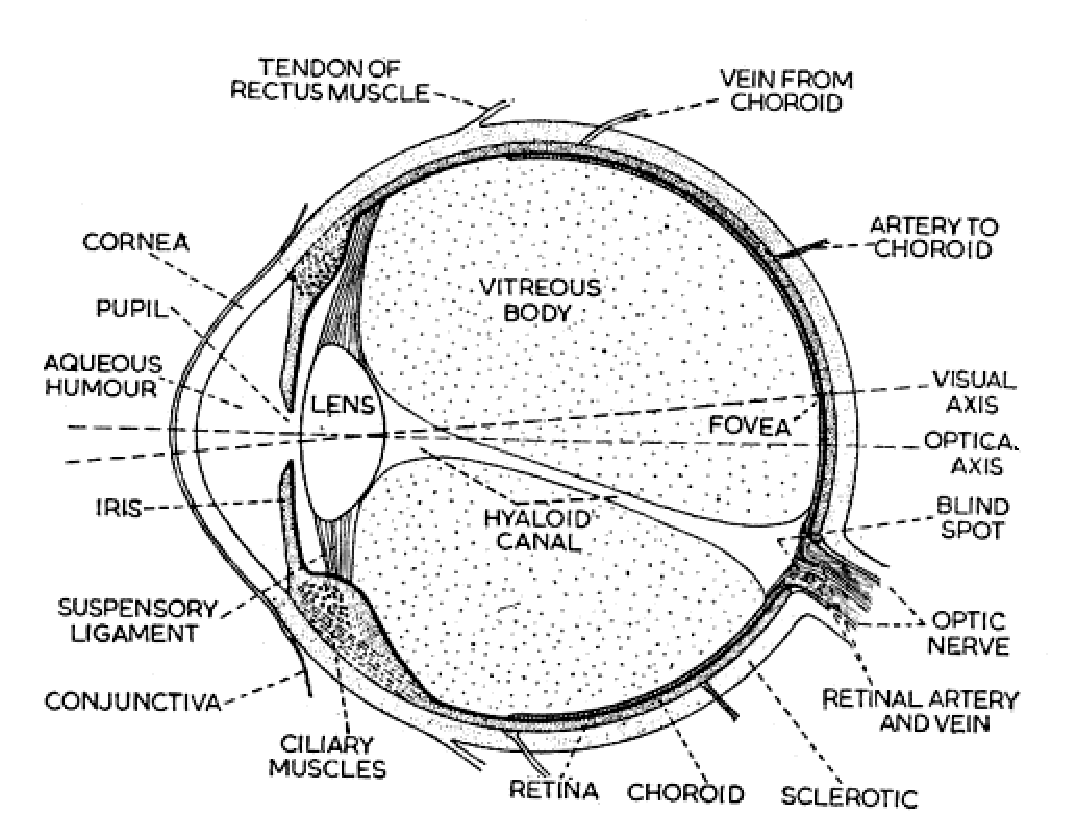
\includegraphics[width=0.49\textwidth]{eye-schematic.eps}
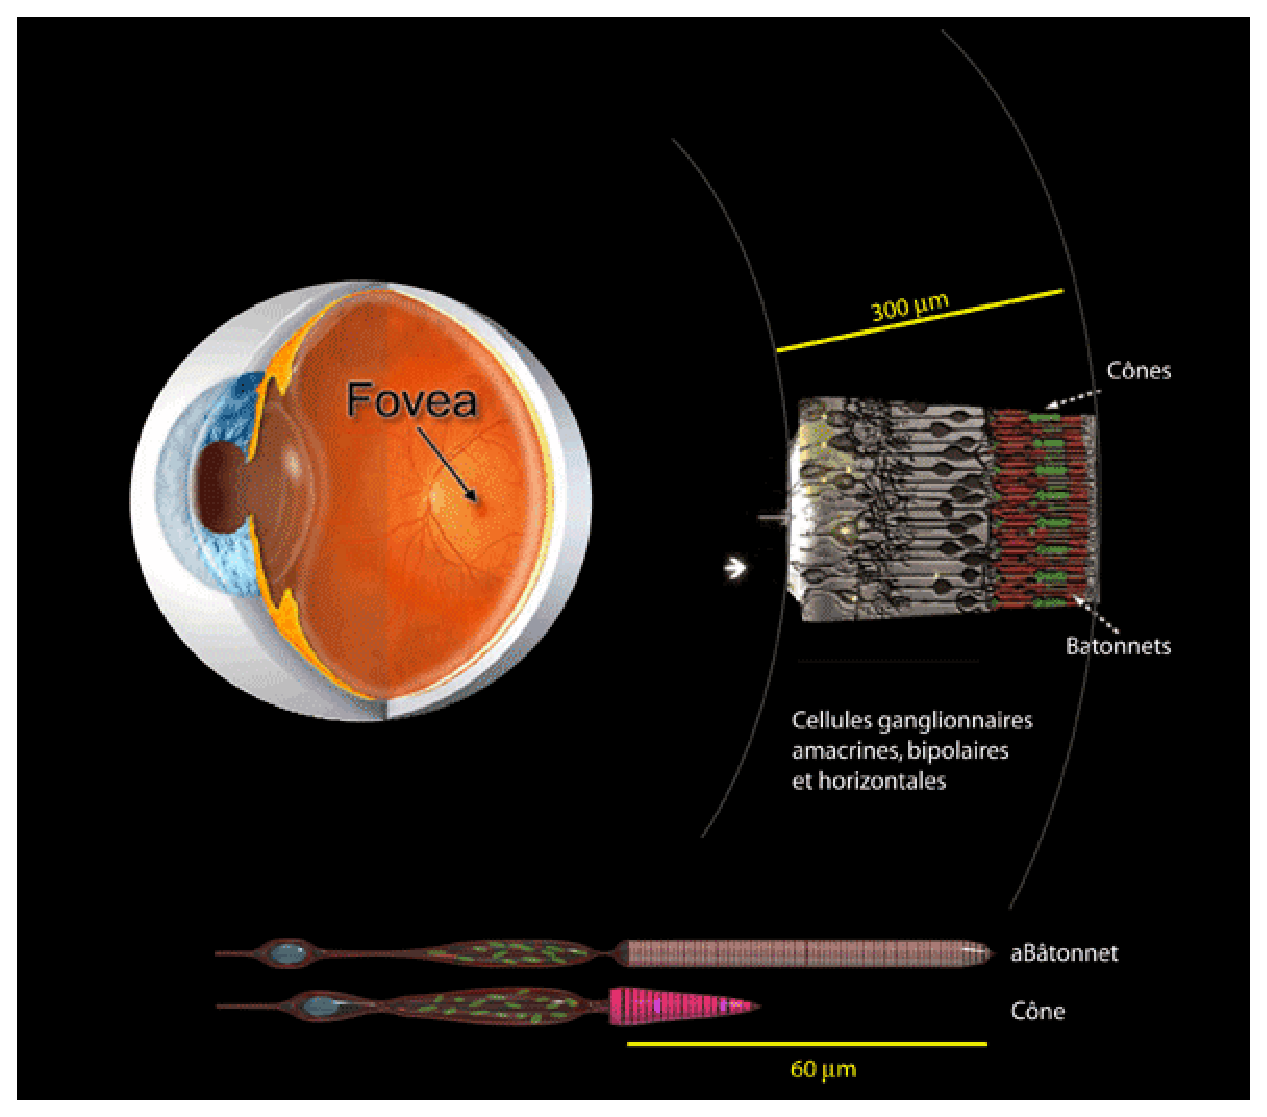
\includegraphics[width=0.49\textwidth]{eye-rod-cone.eps}
\caption{Cross section of the human eye (left), illustration of the eyes
receptor cells; cones, used for color vision with the iodopsin layers 
arranged to the right, and rods with rhodopsin layers. Light enters these
cells from the left before being absorbed by either iodopsin or rhodopsin.}
\end{figure}

Light is focussed on the retina, where there are two types of
receptors: rods and cones. Cones for color reception, rods for black
and white with higher sensitivity. For humans, rods and cones are
arranged {\it backwards} so light must pass through the neuronal wires
that send signals of light back to the brain. In contrast, octopus
eyes, which otherwise are much as our own with a single lens in front
and a light sensitive retina at the back, has the light sensitive
parts of the retinal cells in front. This may be an accident of
nature, or there may be good evolutionary reasons for
the difference. Both designs are mimicked in CCD's used in astronomy,
where {\it thinned, backlit} CCDs are used to avoid unwanted reflections from
the electrodes used to drive them. The CCD in your camera or cell
phone is more probably arranged in the same manner as your eye, with
light having to pass through the electrodes lying on top of light
sensitive doped silicon.

In the rods a pigment known as rhodopsin absorbs radiation. A protein
with a weight of some $40\,000$~amu, arranged in layers 20~nm thick
and 500~nm wide. Under influence of light a small fragment, a
chromophore, will will split off. The chromophore is a vitamin A
derivative called retinal (or retinaldehyde) with a molecular weight
of 286~amu. The portion left behind is a colorless protein called opsin. 
The moment of visual excitation occurs during this break
off process as the cell's electrical potential increases (for
invertebrates on the other hand excitation occurs because the
electrical charge across the membrane is removed). This change in
potential can then propagate along nerve cells to the brain. The
rhodopsin molecule is then (slowly) regenerated. 

The response of cones is similar, but in this case the pigment is
known as iodopsin which also contains the retinaldehyde group. Cone
cells come in three varieties with different spectral sensitivities
(see figure~\ref{fig:absorption-rod-cone}).

In bright light much of the rhodopsin is broken up into opsin and
retinaldehyde, and the rod sensitivity is much reduced so that vision
is primarily provided by the cones, even though their light sensitivity
is only of order 1\% of the rods. The three varieties of cones combine
to give color vision. At low light levels only rods are triggered by
the ambient radiation and vision is then in black and white. 

\begin{figure}[h!]
\centering
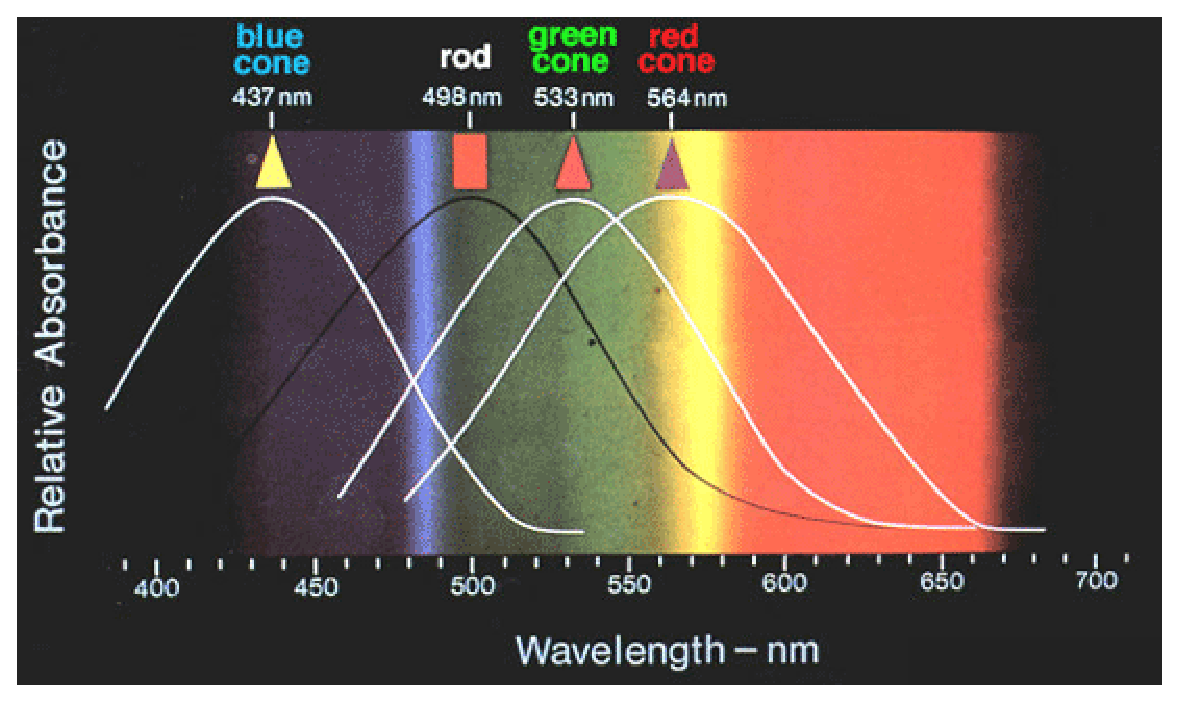
\includegraphics[width=0.66\textwidth]{absorption-rod-cone.eps}
\caption{Absorption curves for the various types of cones, which combined
give color vision, and for rhodopsin. Note that the peak sensitivity
for rods (at 500~nm) and cones (at 555~nm) are at different wavelengths: this causes the
sensitivity of the eye to shift towards blue at low light levels when
the rods dominate.}
\label{fig:absorption-rod-cone}
\end{figure}

Upon entering the dark from a brightly lit region rhodopsin will build
up over a period of roughly 30~min, thus dark-adaptation takes this
long and is based on rod cells. Somewhere between 1--10 photons are
necessary to trigger an individual rod. However, several rods must be
triggered in order to result in a pulse being sent to the brain, as
many rods can be connected to a single nerve fibre. The total number
of rods is of order $10^8$, of cones $6\times 10^6$, these must share
some $10^6$ nerve fibres. Thus there are roughly 100 visual receptors
per nerve fibre, note that there can be many cross connections between
groups of receptors. Cones are concentrated towards the fovea
centralis, which is the region of most acute vision, while rods are
most plentiful towards the periphery of the field of view. Weak
objects are thus most easily visible with averted vision, {\it ie}
when it is not looked at directly. In sum with all these effects the
eye is usable over a range of illuminations differing by a factor
$10^9$ -- $10^{10}$. Note that in regions of high contrast the
brighter region is often seen as too large, this is a phenomena known
as {\it irradiation}. It arises from stimulated responses of unexcited
receptors due to their cross connection with excited receptors. Eye
fatigue occurs when staring fixedly at a source for an extended period
due to depletion of the sensitive pigment.

The Rayleigh limit of the eye, roughly given by $\lambda/D$ where
$\lambda$ is the wavelength of the observed light and $D$ is the size
of the observing aperture, is of order 20~arcsec when the iris has
its maximum diameter of 5--7~mm. However, for two separate images to
be distinguished, they must be separated by at least one unexcited 
receptor cell, so even on the fovea centralis resolution is limited in
practice to between 1~arcmin and 2~arcmin. This is much better than
elsewhere on the retina, since the fovea centralis is populated by
small, tightly packed, singly connected cones. The average resolution
of the eye lies between 5~arcmin and 10~arcmin for point sources. Linear
sources such as an illuminated grating can be resolved down to 1~arcmin.  
The effect of granularity of the retina is countered by rapid oscillations of the
eye through a few 10~arcsec with a frequency of a few Hz, so that
several receptors are involved in the detection when averaged over
time.

The response of the eye to changes in illumination is logarithmic; if
two sources $A$ and $B$ are observed to differ by a given amount, and a
third source $C$ is seen to lie midway between them, then the energy
from $C$ will differ from $A$ by the same factor as it differs from
$B$. The faintest stars visible at a good site (magnitude $6^{\rm m}$)
corresponds to a detection of approximately $3\times
10^{-15}$~W. Sensitivity will vary between individuals and decreases
with age, the retina of a 60~year old person will receive some 30\% of 
the light seen by a person of 30-years.

The system used by astronomers to measure the brightness of stars is a
very old one, and is based on the sensitivity of the eye. Hipparchos'
catalogue of stars divided the stars into six classes from the
brightest, of the first rank or magnitude, to the dimmest of the sixth
magnitude. The present day system is based on this after the work of
Norman Pogson put the magnitude scale on a firm basis in 1856. Pogson
suggested a logarithmic scale that approximately agreed with earlier
measurements: the difference between stars of magnitude $m_1$ and
$m_2$ are given by 
\[
m_1-m_2=-2.5\log\left({E_1\over E_2}\right)
\]
where $E_1$ and $E_2$ are the energies per unit area at the surface of
Earth for the two stars.

\section{Exercises}

\begin{enumerate}
\item What is the size, in kilometers, of the smallest crater that can be distinguished on 
the Moon with the naked eye (as seen from Earth)?
\item Vega has a magnitude of roughly $0.0$, Polaris a magnitude of $2.0$. 
Estimate the magnitudes of the stars in Orions belt as well as Betelgeuse,
Rigel, and Bellatrix. What is the magnitude of the weakest star you can find
in the sky? 
\item Mizar and Alcor in Ursa Majoris are separated by some $11'$.
 Can you separate them and see both stars? Estimate their magnitudes
 as well. Mizar is itself a double star the components of which can be
 separated with a small telescope. Interestingly, all three stars are
 {\it spectroscopic binaries} as well, bringing the star total star
 count up to 6. The distance to these stars is some 83~ly while the
 distance between Mizar and Alcor is approximately
 1~ly. All six stars are  gravitationally bound and are
 members of the Ursa Major moving group.
\end{enumerate}

%\end{document}


% Lecture notes on Chapter 2: Celestial coordinates
%\documentclass{article}
%\usepackage{wasysym}
%\usepackage{graphicx}
%\newcommand{\bc}{\begin{center}}
%\newcommand{\ec}{\end{center}}
%\newcommand{\be}{\begin{equation}}
%\newcommand{\ee}{\end{equation}}
%\newcommand{\bea}[1]{\begin{eqnarray}\label{#1}}
%\newcommand{\eea}{\end{eqnarray}}
%\newcommand{\bua}{\begin{eqnarray*}}
%\newcommand{\eua}{\end{eqnarray*}}
%\newcommand{\dd}[2]{{{d#1}\over{d#2}}}
%\newcommand{\ddt}[1]{\dd{#1}{t}}
%\newcommand{\dddt}[1]{\dd{^2#1}{t^2}}
%\newcommand{\aver}[1]{\langle{#1}\rangle}

%\begin{document}
%\setcounter{section}{1} % No need when combining files I think
\chapter{Celestial coordinate systems}

In order to find something one needs a system of coordinates. For 
determining the positions of the stars and planets where the 
distance to the object often is unknown it usually suffices to use {\it two} 
coordinates. On the other hand, since the Earth rotates around it's 
own axis as well as around the Sun the positions of stars and planets 
is continually changing, and the measurement of {\it when} an object 
is in a certain place is as important as deciding {\it where} it is. 

Our first task is to decide on a coordinate system and the position of
\begin{enumerate}
\item The origin. {\it E.g.} one's own location, the center of the Earth,
the, the center of the Solar System, the Galaxy, etc. 
\item The fundamental plane ($x-y$ plane). This is often a plane of some
physical significance such as the horizon, the equator, or the ecliptic.
\item Decide on the direction of the positive $x$-axis, also known as
the ``reference direction''. 
\item And, finally, on a convention of signs of the $y-$ and $z-$ axes, {\it i.e} whether
to use a left-handed or right-handed coordinate system.
\end{enumerate}

For example Eratosthenes of Cyrene (c. 276 BC –- c. 195 BC) was a Greek mathematician, elegiac poet, athlete, geographer, astronomer, and music theorist who invented a system of latitude
and longitude. (According to Wikipedia he was also the first person to use the word {\it geography} and invented the discipline of geography as we understand it.). The origin of 
this coordinate system was the center of the Earth and the fundamental plane was the 
equator, which location Eratosthenes calculated relative to the parts of the Earth known
to him. 

When viewed from the surface of the Earth the sky above forms a hemisphere, 
astronomical objects are seen to be projected onto this hemisphere. and their 
locations are convenient to describe their location with two angular coordinates in the
same manner as latitude and longitude are decided on the sphere of the Earth. 
Note that the location of the origin of longitude for both the earth and the 
sky are not obvious. In any case, it is necessary to review a few aspects of 
trigonometry on a sphere in order to understand the use of these coordinate 
systems.

Any plane passing through the center of a sphere cuts the surface in a
circle which is called a {\it great circle}. Any other plane that cuts
the sphere, but that does not pass through the center is a {\it small
  circle}. When two great circles intersect at a point they are said
to include a {\it spherical angle} which is defined between the
tangents of the great circles at the point of their intersection. A
spherical angle is only defined with respect to intersecting great
circles.

Given any three points on the surface of a sphere, the sphere can be
bisected so that all three points lie in the same hemisphere. Joining
the points by great circle arcs all in this hemisphere defines a {\it
  spherical triangle}. The length of a great circle arc is defined as
the radius times the angle $A$ formed between the two endpoints of the
arc and the spheres center measured in radians: $R\times A$.

As discussed above there are several methods of specifying a given position on the
celestial sphere, depending on which principal great circles are
chosen as reference. 

%\subsection{Altitude -- Azimuth}
\section{Altitude -- azimuth}

With reference to figure~\ref{fig:alt-az} let $O$, the observer on
the surface of the earth (supposed spherical), be the center of the
celestial sphere. 

\begin{figure}[h]
%{\hfil\psfig{file=alt-az.eps,width=0.66\textwidth}\hfil}
\centering
\includegraphics[width=0.66\textwidth]{alt-az.eps}
\caption{The altitude -- azimuth coordinate system.}
\label{fig:alt-az}
\end{figure}

Let $Z$ be the zenith, vertically overhead be defined by the direction
of gravity. $OZ$ is thus the continuation of the straight line joining
the earth's center to $O$. The plane through $O$ at right angles to
$OZ$ is the plane of the horizon, cutting the celestial sphere in the
great circle $NAS$, called the {\it celestial horizon}. 

Let $X$ be the position of a star on the celestial sphere. Any great
circle drawn through $Z$ is called a {\it vertical circle}; in
particular, the vertical circle through $X$ is $ZXA$. In the plane of
$ZXA$, the angle $AOX$ (or the great circle arc $AX$) is called the
{\it altitude} denoted by $a$. Since $OZ$ is perpendicular to the plane of
the horizon, the great circle arc $ZA$ is 90$^\circ$; hence
$ZX=90^\circ-a$. $ZX$ is called the {\it zenith distance} of the star
$X$. Draw $LXM$ as a small circle through $X$ parallel to the
horizon, it is called the {\it parallel of altitude}. 

To define a stars position completely on the celestial sphere the
particular vertical circle on which it lies must also be
specified. Let $OP$ be parallel to the axis about which the earth
spins. On the northern hemisphere the position $P$ is called the {\it
  north celestial pole}. Due to this rotation the celestial sphere
appears to rotate and the stars to continuously change altitude and
direction. In the northern hemisphere Polaris lies almost directly on
$OP$ and changes direction very little. Define the vertical circle
through $P$ that is $ZPN$ as the principal vertical circle and the
point $N$ as the {\it north point of the horizon}. 

The position of a star $X$ on the celestial sphere at a given moment
is given by reference to the horizon and the principal vertical circle
$ZPN$. If the star is in the western part of the celestial sphere the
spherical angle $PZX$ or the great circle arc $NA$ is called the
{\it azimuth} (W). 

Note that the angle $POZ$ (or great circle arc $PZ$) is equivalent to
the angle between the radius of the earth which passes through the
observer's position and the earth's axis is equal to the co-latitude of
the observer or 
\[ PZ=90^\circ-\phi \]
where $\phi$ is the observers latitude. Hence the altitude of the pole
is equal to the observers latitude.

%\subsection{Some spherical trigonometry}
\section{Some spherical trigonometry}

Both great circle angles and arcs are measured in radians (or
degrees). By definition all angles and and sides in a spherical
triangle are less than $\pi$~radians ($180^\circ$). A spherical
triangle is defined when we know three of its six sides or angles. The
sum of the angles in a spherical triangle is greater than
$180^\circ$, the difference between the sum of the angles and
$180^\circ$ is called the {\it spherical excess}.

Consider a spherical triangle with corners $A,B,C$ on a unit
sphere\footnote{Useful in the following: 
\bua
\cos(\alpha\pm\beta)&=&\cos\alpha\cos\beta\mp\sin\alpha\sin\beta \\
\sin(\alpha\pm\beta)&=&\sin\alpha\cos\beta\pm\cos\alpha\sin\beta
\eua}. Assume that these corners follow each other in the positive sense.
The sides $a,b,c$ lie directly opposite these corners.
Insert a right handed coordinate system $x,y,z$ with origin at the
sphere's center, let the $z$ axis go through the point $A$, and the
$x-z$ plane through the side $c$. The coordinates of the corner $C$ are then 
\begin{eqnarray}
z & = & \cos b \nonumber \\
x & = & \sin b \cos A \nonumber\\
y & = & \sin b \sin A. 
\label{eq:sph-unmark}
\end{eqnarray}
Now rotate the coordinate system around the $y$-axis until the
$z$-axis goes through $B$. Call the new coordinate system
$x',y',z'$ (see figure~\ref{fig:sph-trig}). 
The corner $C$'s coordinates in the new system are then -
since we see that the side $a$ is equivalent to $b$ in the old system
and the angle $\pi-B$ is equivalent to $A$:
\begin{eqnarray}
z' & = & \cos a \nonumber \\
x' & = & -\sin a \cos B\nonumber \\
y' & = & \sin a \sin B. 
\label{eq:sph-mark}
\end{eqnarray}

\begin{figure}[h]
%{\hfil\psfig{file=sph-trig.eps,width=0.66\textwidth}\hfil}
\centering
\includegraphics[width=0.66\textwidth]{sph-trig.eps}
\caption{Two axis systems used to derive the basic formula of spherical
trigonometry.}
\label{fig:sph-trig}
\end{figure}

To find the relation between the marked and unmarked coordinates, put
a plane through the $x-z$ axes. On rotation the $y$-coordinate is
unchanged. With reference to figure~\ref{fig:sph-trig} we see the
following relations:
\[
\begin{array}{cccc}
v'=v-c \qquad& z=\cos v\qquad  & x=\sin v \qquad& \qquad\\
       & z'=\cos v'\qquad& x' =\sin v'\qquad & \qquad
\end{array}
\]
Now express $z'$ and $x'$ with the help of $v$ and $c$
\begin{eqnarray}
z' & = & \cos v \cos c + \sin v \sin c\nonumber \\
x' & = & \sin v \cos c - \sin c \cos v,\nonumber
\end{eqnarray}
setting in for $z$ and $x$ and remembering that $y$ is unchanged gives
\begin{eqnarray}
z' & = & z\cos c + x \sin c \nonumber \\
x' & = & x \cos c - z \sin c \nonumber \\
y' & = & y. 
\label{eq:sph-translate}
\end{eqnarray}
Setting in equations~\ref{eq:sph-unmark} and \ref{eq:sph-mark} in
equation~\ref{eq:sph-translate} gives the basic formulae of spherical
trigonometry:
\begin{eqnarray} 
\cos a &=& \cos b\cos c+\sin b\sin c\cos A \\
\sin a \cos B &=& \sin c \cos b-\cos c\sin b\cos A\\
\sin a \sin B &=& \sin b \sin A
\end{eqnarray}
The first of these is the {\it cosine formula}, the second the {\it
  sine--cosine} formula, and the third the {\it sine} formula.

%\subsection{Declination -- hour angle}
	\section{Declination -- hour angle}

Consider now again the celestial sphere as drawn in figure~\ref{fig:hr-dec}.

\begin{figure}[h]
%{\hfil\psfig{file=hr-dec.eps,width=0.66\textwidth}\hfil}
\centering
\includegraphics[width=0.66\textwidth]{hr-dec.eps}
\caption{Relation between altitude -- azimuth and declination -- hour angle
coordinates.}
\label{fig:hr-dec}
\end{figure}

The great circle $RWT$ whose plane is perpendicular to $OP$ is the
{\it celestial equator} and its plane is parallel to that of the
earth's equator. The celestial equator and the horizon intersect in
two points $W$ and $E$. Now $Z$ is the pole of the great circle $NWS$
and $P$ is the pole of the great circle $RWT$; hence $W$ is $90^\circ$
from both $Z$ and $P$ and therefore $90^\circ$ from all points on the
great circle through the great circle through $Z$ and $P$. This means
that $W$ is the pole of the great circle $NPZQ$; hence $NW=90^\circ$
and $WS=90^\circ$. Similarly  $EN=90^\circ$ and  $ES=90^\circ$. Thus
$W$ and $E$ are the remaining {\it cardinal points}, in addition to
$N$ and $S$. 

The rotation of the earth results in an apparent rotation of the
celestial sphere from east to west about $OP$. As stars are {\it very}
far from the earth, the angle between the straight line joining the
observer at $O$ to any particular star and the straight line $OP$
remains unaltered. The earth's rotations makes the star $X$ describe a
small circle $LXM$, parallel to the celestial equator. Let $PXDQ$ be
the semi-great circle through $X$ and the poles of the celestial
sphere. Then $DX$ is called the {\it declination} of the star and is
{\it north declination} if the star is between the celestial equator and
the north pole. Denoting the stars declination $DX$ by $\delta$ and
$PX=90^\circ-\delta$ is called the {\it north polar distance} of the
star. 

When we know the declination of a star, a small circle, {\it the
  parallel of declination}, is defined. In order to completely
specify the stars position we need another great circle of
reference. This is the semi-great circle $PZRSQ$ called the {\it
  observer's meridian}. When the star is at $L$ on the observers
meridian it is is said to {\it transit} or {\it culminate} at which
time it is at its greatest altitude. Afterward the star moves along
the small circle $LFM$ crossing the horizon at $F$, when it is said to
{\it set} with an altitude of $0^\circ$. Eventually it will pass through
its position of maximum depression at $M$ before continuing on to $G$
where the altitude again is $0^\circ$ and is said to {\it rise}. At
any moment the star's position on the parallel of declination is
specified by the angle $P$ between the observer's meridian and the
meridian ($PXQ$) through the star at this time; this angle is $RPX$ or
arc $RD$ on the equator. This angle, denoted by $H$, is called the
{\it hour angle} and is measured from the observer's meridian {\it
  westwards} from $0^\circ$ (at $L$) to $360^\circ$ (when the star
returns to the observer's meridian), or more usually from $0^h$ to 
$24^h$. 

%\subsection{The standard geocentric celestial sphere}
\section{The standard geocentric celestial sphere}


For stars, which are very far away, the position of the observer on
the surface of the earth is irrelevant to the definition of the stars
position. But when we are considering a relatively nearby object such
as the moon, the sun, or a planet the definition of the north polar
distance (and therefore of declination) previously given {\it is}
dependent on position of the observer on the earth. 

Accordingly, the center of the standard celestial sphere is taken to
be at $C$ the earth's center. 

%\subsection{Right ascension and declination}
\section{Right ascension and declination}

In the hour angle and declination method of specifying a star's
position on the celestial sphere only one coordinate, the declination,
remains constant as the start travels across the sky. 

\begin{figure}[h]
%{\hfil
\psfig{file=ra-dec.eps,width=0.66\textwidth}\hfil}
\centering

\includegraphics[width=0.66\textwidth]{ra-dec.eps}
\caption{Definition of the right ascension -- declination coordinate system.}
\label{fig:ra-dec}
\end{figure}

Let us now pick a point $\aries$ on the celestial equator and let the
meridian through the star $X$ cut the celestial equator at $D$. As the
stars pass across the sky the declination $DX$ remains constant and
that the relative configuration of the stars also remain constant. It
follows that $\aries D$ is constant. We regard $\aries$ as a reference
point on the celestial equator; we can then clearly specify the the
position of the star $X$ by means of the great circle arc $\aries D$
and the declination $DX$. The reference point chosen is called the
{\it vernal equinox} or the {\it first point of Aries}. The arc
$\aries D$ is called the {\it right ascension} ({\sc r.a.}) of the
star $X$. It is denoted by $\alpha$ and is measured {\it eastward}
from $\aries$ from $0^h$ to $24^h$, opposite to the direction the hour
angle $H$ is measured. 

Note that $R\aries =RD+\aries D$. The hour angle of $\aries$ is called
the {\it sidereal time}\footnote{{\bf sidereal}: of or with respect to distant stars.} 
 ({\sc s.t.}). We have accordingly 
\[
{\rm S.T.}=H+\alpha
\]
When $\aries$ is on the observer's meridian, the hour angle of
$\aries$ is $0^h$, {\it i.e} the sidereal time is $0^h$. When $\aries$
is next on the observer's meridian an interval of $24^h$ of sidereal
time has elapsed. This interval is the same as is required for the
complete revolution of the earth about its axis and is called a {\it
  sidereal day}. 

%\subsection{The earth's orbit}
\section{The earth's orbit}

According to Kepler's first law of planetary motion, the earth is a 
planet revolving around the sun in an elliptical path or orbit, and
the sun is situated in a focus of the ellipse. Since our observations
are made from earth, then relative to the earth the sun appears to
describe an elliptical path around the earth. In the course of a year
the sun makes a complete circuit of the heavens against the background
of the stars. The plane of the orbit is called the {\it plane of the
  ecliptic},  and the great circle in which this plane intersects the
celestial sphere whose center is the earths center $C$, is called the 
{\it ecliptic}. With reference to the stars, the plane of the ecliptic
will be a particular great circle which is found by observations to be
inclined at an angle of about $23{1\over 2}^\circ$ to the celestial
equator. 

\begin{figure}[h]
%{\hfil\psfig{file=ecliptic.eps,width=0.66\textwidth}\hfil}
	\centering
	\includegraphics[width=0.66\textwidth]{ecliptic.eps}
	\caption{Celestial longitude and latitude.}
	\label{fig:ecliptic}
\end{figure}

In figure~\ref{fig:ecliptic}, $Y\aries M$ represents the ecliptic and
its inclination to the celestial equator is $M\aries R$, which is
known as the {\it obliquity of the ecliptic}. Relative to the earth,
the sun appears to move on the celestial sphere along the ecliptic in
the direction $Y\aries M$ and twice yearly its position coincides
with the intersections of the ecliptic with the celestial equator. The
position $\aries$, at which the sun's declination changes from south
to north, is the {\it vernal equinox}. It is in this way that the
reference point $\aries$ is obtained, from which the right ascension
of stars is measured. From the diagram it is seen that the right
ascension and declination of the sun are both changing
continually. When the sun is at $\aries$ its right ascension and
declination are both zero (this occurs roughly March 21); at $M$ the
right ascension is $6^h$ and declination about $23 {1\over2}^\circ$~N
(roughly June 21, summer solstice); at $U$ the right ascension is
$12^h$ and declination $0^\circ$ (September 21, autumnal equinox),
and at $Y$ the right ascension is $18^h$ and the declination about $23
{1\over 2}^\circ$~S (December 21, winter solstice).

\section{Celestial latitude and longitude}

The position of a heavenly body can also be referred to the ecliptic
as fundamental great circle and the vernal equinox $\aries$ as principal
reference point. E.g. in figure~\ref{fig:ecliptic}, $K$ is the north pole
of the ecliptic and $KXA$ is a great circle arc passing through $X$
and meeting the ecliptic in $\Lambda$. The arc $\aries\Lambda$,
measured from $\aries$ along the ecliptic in the direction of the
sun's annual motion (eastwards), is called the {\it longitude} of $X$
and is measured from $0^\circ$ to $360^\circ$ round the ecliptic. The
arc $\Lambda X$ is the {\it latitude}, north is considered positive
and south negative. 

Thus, if one know a star's right ascension and declination it is
possible to obtain its latitude ($\beta$) and longitude ($\lambda$)
from the triangle $KPX$; and vice versa.

\section{Sidereal time {\sc i}}
\label{sec:sidereal_time_i}

Sidereal time at Greenwich is given such that
\[
{\rm S.T.~at~Greenwich}={\rm S.T.~at}~l\pm{\rm long.~of~}l
\]
where $l$ is the longitude of the observer with the $+$ sign given
when $l$ is west of Greenwich and the $-$ is given when $l$ is east of
Greenwich. The sidereal time at $l$ is called the {\it local sidereal
  time} ({\sc l.s.t.}).

\section{Mean solar time}

When the sun is on the meridian of a given place, it is apparent {\it
  noon} there; when the sun is next on the meridian, an {\it apparent
  solar day} has elapsed. An apparent solar day is not constant --- due
to the fact that the sun's apparent orbit around the earth is not a
circle but rather an ellipse. In addition the sun moves along the
ecliptic and not the celestial equator so it's right ascension does
not increase uniformly. The average apparent solar day through the
year is called a {\it mean solar day}. The mean sun is assumed to
move in the {\it celestial equator} at a uniform rate around the
earth. The rate is such that the mean sun completes its orbit in the
same amount of time as the real sun needs to complete an orbit around
the ecliptic. Assume that the right ascension of the sun is known,
then 
\[
{\rm Sid. time}={\rm H.A.M.S.}+{\rm R.A.M.S}
\]
The mean sun is related to the true sun by certain principles that
will be discussed later; for now let us define the difference as the
{\it equation of time} $E$ such that
\[
E={\rm R.A.M.S-R.A.\astrosun}
\]
$E$ can be positive or negative and varies in a complicated manner. 

When the mean sun is on the meridian of Greenwich, it is {\it Greenwich
  mean noon}. The hour angle of the mean sun at Greenwich is denoted
{\sc g.m.a.t.} ({\it Greenwich mean astronomical time}). 
Mean time reckoned from midnight at Greenwich is called
{\it Greenwich Mean Time} ({\sc g.m.t.}), now designated {\it
  Universal Time} ({\sc u.t.}). Thus
\[
{\rm U.T.}\equiv{\rm G.M.T.}={\rm G.M.A.T.}+12^h
\]
and similarly for any place keeping the mean time appropriate to its
meridian. 

\section{Sidereal time {\sc ii}}

Sidereal time, at any instant at a given place, is the hour angle of the vernal 
equinox. In section~\ref{sec:sidereal_time_i} the ecliptic and celestial equator were 
considered as fixed great circles on the celestial sphere, and thus the vernal
equinox as a fixed point. However, there are both the phenomena of {\it 
precession} and {\it nutation}\footnote{{\bf precession}: the slow movement of the axis of a spinning body around another axis due to a torque acting to change the direction of the first axis. {\bf nutation}: a periodic variation in the inclination of a rotating object.}  so the celestial equator cannot be considered 
as a fixed great circle, and the position of the vernal equinox must be treated as
a time varying quantity, slowly moving according to well established principles with
reference to the background stars.

\begin{figure}[h]
%{\hfil\psfig{file=sidereal.eps,width=0.66\textwidth}\hfil}
	\centering
	\includegraphics[width=0.66\textwidth]{sidereal.eps}
	\caption{Definition of sidereal time and the effects of precession; motion 
		of the vernal equinox. }
	\label{fig:sidereal}
\end{figure}

We will continue to assume the ecliptic as a fixed great circle. Owing to precession, 
the north celestial pole $P$ describes a small circle about the pole $K$ (see 
figure~\ref{fig:ecliptic}) of the ecliptic in a period of about $26\,000$~yr. At 
present $P$ is within $1^\circ$ of the star $\alpha$ Ursae Minoris (Polaris), but 
their relative positions are changing and in $12\,000$~yr  $P$ will be within a few
degrees of Vega. It is the direction of the earth's axis that is altering continuously 
with reference to the background stars. Referring to figure~\ref{fig:sidereal},
$\aries$ is the vernal equinox for, say $1900.0$ and $\aries_1$ the vernal equinox
for $1901.0$. \aries\ and $\aries_1$ are called the {\it mean equinoxes} at the dates
in question, and the corresponding celestial equators are called the 
{\it mean equators}. 

Assuming that owing to precession the north celestial pole moves uniformly along the 
small circle arc $PP_1$ and that the mean equinox moves uniformly backwards along the 
ecliptic from from \aries\  to $\aries_1$. It is found that the motion of \aries\  along
the ecliptic is at the rate of $50.3$~arcsec per annum.

When we define sidereal time in relation to the moving equinox, we can no longer 
regard the earth's rotational period to be the interval between two successive transits
of the equinox. In figure~\ref{fig:sidereal} let $C\aries_1$ be a great circle arc
drawn through $\aries_1$ perpendicular to the equator. Then the equinox at any given 
date is separating, in right ascension, from the equinox \aries\  for $1900.0$ at a the
annual rate measured by $\aries C$, given by the small triangle formula
\[ 
\aries C=\aries\aries_1\cos\varepsilon.
\]
Hence, the mean equinox is separating, in right ascension, from \aries\  at the rate
of $0.008$~s per sidereal day. The direction of motion of the equinox is westward 
in the sky --- opposite to that in which right ascension increases --- and thus the 
interval between two successive transits of the moving equinox is $0.008$~s less than 
the interval given by a fixed equinox. This first interval is a {\it sidereal day}, 
the second interval is the rotational period of the earth.

Owing to nutation the true equator at any instant is slightly different from the 
mean equation at that instant. Consequently the true equinox is displaced slightly 
along the ecliptic relative to the mean equinox; these displacements are periodic
in nature (and due the effect of the moon), with a period of about 18~yr. 
The difference in right ascension between the true equinox and the mean equinox due 
this effect can amount to 1.2~s

One defines {\it mean sidereal time} to associated with the moving mean equinox 
(only precession considered) and {\it apparent sidereal time} to be associated 
with the true equinox. The difference between these from day to day is so small
in practice that generally the sidereal day is taken to mean the interval between
two successive transits of the mean equinox.

\section{Ephemeris and Universal time}

There is a slight distinction between universal time, which is defined by the 
rotation of the earth and {\it ephemeris time} which is uniform and is defined
by the gravitational dynamics of the solar system, independent of the earth's 
rotation.

When the movements of the equator and equinox due to precession are taken into
account, the {\it fictitious mean sun} is defined to travel along the mean 
equator in such a way that that its mean right ascension is always equal to 
the sun's mean longitude. This right ascension is, therefore, independent 
of the rotation of the earth's, and the fictitious mean sun is a 
suitable reference point for the definition of ephemeris time. To 
facilitate this an alternate meridian is defined called the ephemeris 
meridian which corresponds to the sidereal direction that the
Greenwich meridian would have if the earth were rotating strictly uniformly. 
Ephemeris time is defined as 
\[
{\rm E.T.}=12^h+{\rm E.H.A.F.M.S.}
\]
where the last term of the right hand side is the ephemeris hour angle of the 
fictitious mean sun. 

In contrast, a slightly different reference point, the mean sun,
is used to define universal time. The mean sun also moves round the mean 
equator but at a rate that is directly proportional at each instant to the 
earth's angular velocity. 

\section{Terrestrial Time and Barycentric Coordinate Time}

Astronomers stuck with ephemeris time until 1979, when they defined two new 
time scales that used the atomic second and that took into account 
relativity (velocity affects time). From 1 January 1984, these scales 
replaced ephemeris time in national ephemeris like the Nautical Almanac.

Terrestrial Dynamical Time (TDT) views time from the earth's position and 
motion. It was defined as being equal to TAI (Atomic time) plus 
32.184 (atomic) seconds at the instant beginning 1 January 1977.

Barycentric Dynamical Time (TDB, from the French) is time at the center of 
mass of the solar system. TDB has various forms depending on the theory of 
relativity adopted.

By International Astronomical Union (IAU) Resolution A4 in 1991, 
Terrestrial Dynamical Time was renamed Terrestrial Time (TT). 
Recommendations III and V of the same resolution created 
Barycentric Coordinate Time (TCB) to take the place of Barycentric 
Dynamical Time, except in situations where maintaining continuity in 
ongoing work made retaining the old scale preferable.

In 2006 (Resolution B3)
\footnote{
%\begin{verbatim}
\tt www.iau.org\/static\/resolutions\/IAU2006\_Resol3.pdf
%\end{verbatim}
}
, responding to the ``multiple realizations of TDB''
and other factors, the IAU defined TDB in terms of TCB. One result is that, 
within a few thousand years around the present, the difference between 
Terrestrial Time and Barycentric Dynamical Time on the surface of the Earth 
is less than 2 milliseconds. 

\section{The sidereal year and the tropical year}

The time required by the sun to make a complete a complete circuit of the 
ecliptic is called a {\it sidereal year}. 

The {\it tropical year} is the average interval between two consecutive 
passages of the sun through the vernal equinox. Thus if \aries\ is the 
position of the equinox
at a given time and $\aries_1$ the position of the equinox one year later, the 
tropical year is the time taken by the sun to describe $360^\circ$ less 
$\aries_1\aries$. From observations it is found to be $365.2422$~days. 

The relation between the sidereal year and the tropical year is then evidently
\[ 
{{\rm Sid.~year}/{\rm trop.~year}}={360^\circ/{(360^\circ-50.3'')}}
\]
This gives a sidereal year of $365.2564$~days.

During the course of a tropical year the {\sc r.a.m.s} increases from $0^\circ$ to
$360^\circ$, that is at the rate of $360^\circ/365.2422$ or $59'8.33''$ per mean 
solar day. Let $t_1$ be the mean sidereal time when the hour angle of the mean sun
at a given place is $H_1$ and let $R_1$ denote the corresponding value of 
the {\sc r.a.m.s.}. Then
\[
t_1=H_1+R_1
\]
Let $t_2$ be the mean sidereal time one mean solar day later. The hour angle of 
the mean sun has increased by $360^\circ$ and the {\sc r.a.m.s} by $59'8.33''$.
Hence,
\[
t_2=(H_1+24^h)+(R_1+3^m56.556^s)
\]
when we convert these to time measure, so that 
\[
t_2-t_1=24^h3^m56.556^s
\]
This means that $24^h$~{\sc u.t.} is equal to $24^h3^m56.556^s$ mean sidereal time.
Note that this is equivalent to noting that during a year the earth has rotated about
its axis $365.2422$ times with respect with the mean sun and once more with respect
to the equinox.

\section{The Besselian year}

It is the general astronomical practice to define the beginning of the tropical year
(sometimes called the solar year) as the instant when the {\sc r.a.} of the fictitious
mean sun is exactly $18^h40^m$ or $280^\circ$. This instant falls near the beginning of
the civil year and is usually called the {\it Besselian year}. 

It is general practice to denote the beginning of any Besselian year by the notation
{\it e.g.} $1975.0$, $2008.0$, etc.

\section{The Julian date}

In certain observations it is found convenient to express the instant of observations
as so many days and fraction of a day after a definitive fundamental epoch. The epoch
chosen is Greenwich mean noon of January 1, 4713~{\sc b.c.}, and for any given date the
number of days which have elapsed since this epoch defines the {\it Julian Date} 
({\sc j.d.}) of the date in question.

\section{The 3d dimension; distance}

Determining the distance to astronomical objects is very difficult, and was for a very
long time one of astronomy's largest unsolved problems. Hence, even today, the uncertainty 
in measuring distance is enormous compared to uncertainties in direction. For example,
the position of Alpha Centauri is uncertain in the ICRS (the International Celestial Reference
System) by about 0.4~mas (milliarcsec), which amounts to 3 parts in $10^9$ of a full circle, while
its distance is uncertain by about one part in $2500$. 

\subsection{The astronomical unit}

Kepler's 3'd law gives the scale of planetary orbits

\[ a=P^{2/3} \]

where $P$ is the period measured in years, and $a$ is the distance of a planet (or other object) 
measured in units of the average distance between object and the Sun which defines the 
astronomical unit; AU, or au. The presently accepted value for this length is
\[ 1~{\rm au}=1.49\,5978\times 10^{11}~{\rm m} \]
with an ancertainty of one part in $10^6$.

\subsection{Stellar parallax}

Once the length of the au has been established one can measure the distances to the nearby stars
through the obsrvation of {\it stellar parallax}. As the Earth travels in its orbit the apparent
position of a nearby star relative very distant objects shifts. Compared to background objects,
the nearby star appears to move around the perimeter of the prallactic ellipse, reflecting the 
Earth's orbital motion. The parallax angle $p$ is half the total angular shift in the star's
position (the semi-major axis of the parallactic ellipse). From the right triangle formed by the
Sun-star-Earth:
\[ \tan p={a\over r} \]
where $a$ is one au and $r$ is the distance to the star. Since $p$ is very small, a very good 
approximation is \[\tan p\simeq\sin p\simeq p\] so that \[ p={a\over r}\]. Usually one measures
$p$ in arcsec so that 
\[ p[{\rm arcsec}]=206\,265{a\over r}. \]
To avoid very large numbers it is both convenient and traditional to define the unit parsec with 
the length
\[ 1~{\rm parsec}=206\,265~{\rm au}=3.085\,678\times 10^{16}~{\rm m}=3.261\,633~{\rm ly}. \]
The parsec (pc) is named because it is the distance of an object whose parallax is one arcsec. 
In the literature the parallax angle is often symbolized $\pi$ instead of $p$.

{\it Some history:} James Bradley FRS (March 1693 -– 13 July 1762) was an English astronomer the Astronomer Royal from 1742. He undertook to measure stellar parallax. Bradley could measure stellar positions with a precision of about 0.5~arcsec (500~mas). This was good enough to
discover both the effects of aberration of light (1725 –- 28), and the nutation of the Earth's axis (1728 –- 48), but not good enough to measure the parallax of stars.

Some generations later Friedrich Bessel (1784 -- 1846) studying Bradley's observations discoverd
that major advances in positional accuracy could be accomplished. He undertook a campaign to
monitor the double star 61~Cygni along with two background stars. In 1838, after a 25~year effort(!), he succeeded in measuring its parallax to 320~mas, close to the modern value of 
286~mas. Other scientists trying to measure stellar parallax at about the same time were
William Struve in St. Petersburg who measured Vega, and Thomas Henderson in South Africa who measured Alpha Centauri; of these Bessel's measurement was the most accurate.

\section{Exercises}

\begin{enumerate}
\item Given the observers latitude $\phi$, the declination $\delta$
  and hour angle $H$ of the heavenly body, calculate the zenith
  distance $z$ and the azimuth $A$.
\item Given the observer's latitude $\phi$, the stars zenith distance
  and azimuth, calculate the star's declination and hour angle.
\item Work out a stars latitude ($\beta$) and longitude ($\lambda$)
  given its declination ($\delta$), right ascension ($\alpha$) and the
  obliquity of the ecliptic ($\varepsilon$).
\item Use {\tt IDL} or {\tt Matlab} to produce a figure of 
altitude as function of
hour angle for stars observed from Oslo with declinations of
-30,-15,0,+15,+30,+45,+60 degrees (all in the same figure).
\item Use {\tt IDL} or {\tt Matlab} 
to produce a figure of altitude as function of
azimuth for the same stars (also as observed from Oslo).
\end{enumerate}

%\end{document}


% Lecture notes on Chapter 3: Detectors
%\documentclass{article}
%\usepackage{wasysym}
%\usepackage{graphicx}
%\newcommand{\bc}{\begin{center}}
%\newcommand{\ec}{\end{center}}
%\newcommand{\be}{\begin{equation}}
%\newcommand{\ee}{\end{equation}}
%\newcommand{\bea}[1]{\begin{eqnarray}\label{#1}}
%\newcommand{\eea}{\end{eqnarray}}
%\newcommand{\bua}{\begin{eqnarray*}}
%\newcommand{\eua}{\end{eqnarray*}}
%\newcommand{\dd}[2]{{{d^2#1}\over{d#2^2}}}
%\newcommand{\aver}[1]{\langle{#1}\rangle}
%\def\cl#1{{\cal #1}}               % for caligrafic letters
%\def\abs{\!\mid\!}
%\def\labs{\mid\!}
%\def\rabs{\!\mid}
%\def\rd{\mbox{d}}
%\def\rD{\mbox{D}}
%\begin{document}
\chapter{Detectors}

\section{Detector parameters}

The overall performance of a detector (CCD or other) is described in terms of
different technical parameters. A short-list of such parameters
include:

\begin{itemize}
  \item The {\em quantum efficiency} (QE) is the ratio of the actual
  number of photons detected to the number of incident photons. This
  quantity varies with wavelength. In the range 300-900~nm typical
  values fall in the range 0.2--0.75 with maximum efficiency around 
  500~nm.  
  \item The {\em spectral response} is the change in the output
  signal as a function of the wavelength of the input signal.
  \item The {\em charge transfer efficiency} (CTE) specifies the 
  efficiency at which accumulated charge may be transfered from one 
  pixel to the next. For a 1~\% accuracy in the read-out process 
  for a 10000 element detector a 99.9999~\% transfer efficiency is
  required. Actual numbers as high as 99.99999~\% have been quoted.
  \item The {\em dark current} represent the output from the
  non-illuminated detector. It is usually measured as a
  root-mean-square current.  
  \item The {\em dynamic range} is the ratio of the saturation output
  to the dark current.  
  \item The {\em  noise equivalent power} (NEP) is the input radiative 
  flux that gives
  a signal-to-noise ratio of unity. It may be given for monochromatic
  or black body radiation. It is usually measured in watts.  
  \item The  {\em detectivity} (D) is the inverse NEP value, that is, the
  signal-to-noise ratio for unity intensity input radiation.  
  \item  The {\em normalized detectivity} (D$^*$) is the detectivity
  normalized by multiplying with the square root of the product of the
  detector area and the electrical bandwidth of the measuring
  circuitry 
  \begin{equation} 
    D^* = \frac{(A \Delta f)^{1/2}}{NEP}.
    \label{CCD.Dstar}
  \end{equation}
  The usual unit is cm Hz$^{1/2}$ W$^{-1}$.
\end{itemize}

The technical specifications for the CCD are improving year by
year. Instead of dwelling further on such specifications or the
practical challenges met with in the fabrication process of such
devices, we will therefore turn to a discussion of the physical
principles behind the working detector. This will require knowledge of
basic properties of solid state conductors, insulators, and
semi-conductors, the photo-electric effect, and the
metal-oxide-semiconductor (MOS) capacitor.

\section{Semiconductors}

Many types of detectors base their properties on those of {\it
  semiconductors}. Thus, let us discuss these properties as a
prerequisite to achieving an understanding of the detectors that
employ them. 

For a single many-electron atom the Pauli principle requires the
electrons to occupy different electron states. This principle also
applies to the total number of electrons in a solid block of
material. Instead of the discrete energy levels of the single atom,
the solid block displays a series of continuous energy bands available
to the electrons. Energy bands for which every allowed electron state
is occupied at zero temperature are called valence bands, energy bands
that are only partially filled are called conduction bands. 

From statistical mechanics the probability distribution function for
finding a given energy level $U$ occupied by an electron (of spin 1/2)
is given by the Fermi-Dirac distribution function
\begin{equation}
  f_{FP}(U) \sim \frac{1}{1+\exp((U-U_F)/\cl T)},
  \label{CCD.fFD}
\end{equation}
where $\cl T$ is the temperature (in energy units, $\cl T = \kappa T$
where $\kappa$ is the Boltzmann constant and $T$ temperature in
degrees Kelvin) and $U_F$ is the Fermi energy. The Fermi-Dirac
distribution function (\ref{CCD.fFD}) is displayed in figure
\ref{CCD.figfFD}. At $\cl T = 0$ all energy levels up to $U_F$ are
occupied. At finite temperatures a definite variation of $f_{FD}$ with
$U$ is found only for $\labs U - U_F \rabs$-values up to order $\cl
T$. We note that $U_F$ represents the average energy acquired by an
extra electron introduced to the material block under conditions of
constant temperature. With the zero of the energy scale referred to the
usual infinity of vacuum electrostatics, the Fermi energy is also
referred to as the electro-chemical potential of the electron.

\begin{figure}[h]
  \centering
	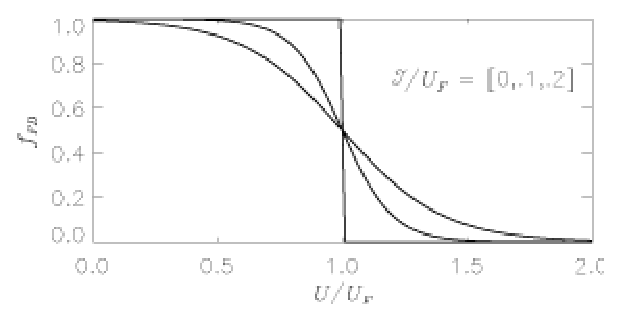
\includegraphics{CCD_fFD.eps}
  \caption{The Fermi-Dirac distribution function}
  \label{fig:CCD.figfFD}
\end{figure}

If an electric field is imposed on the material, the electrons will
tend to move. In this process the energy of the electron must
increase, the extra energy later to be expended in collisions with
other electrons or sound generation, and leading to the Ohmic heating
of the material. For an electron to increase its energy, however, a
suitable empty local energy level must be available. In the absence of
such energy levels the electron is not allowed to move. In metals with
a partly filled conduction band there is ample supply of such empty
energy levels, the conduction band electrons are free to move. The
metals are therefore good electrical conductors, with the electrical
conductance generally decreasing with temperature. In figure
\ref{CCD.figsolstate} valence band energy levels are drawn blue,
conduction band levels red. Filled levels are illustrated with
solid lines, empty levels by dashed lines. 


Now consider a material made from group IV atoms like carbon (C),
silicon (Si) or germanium (Ge).  These atoms each make covalent
bindings with their four nearest neighbors. This results in filled
valence bands and an empty conduction band.  For diamond (C) the
energy gap between the top of the valence band $U_V$ and the bottom of
the conduction band $U_C$ is of the order of 6 to 7 eV, much larger
than the typical thermal energy of the topmost electrons. Thus, the
conduction band remains empty and there are no available local energy
levels for electrons in the filled valence band to move to under
influence of the electric field. The electrons are thus not allowed to
move and the material will be an insulator.

\begin{figure}[h]
	\centering
	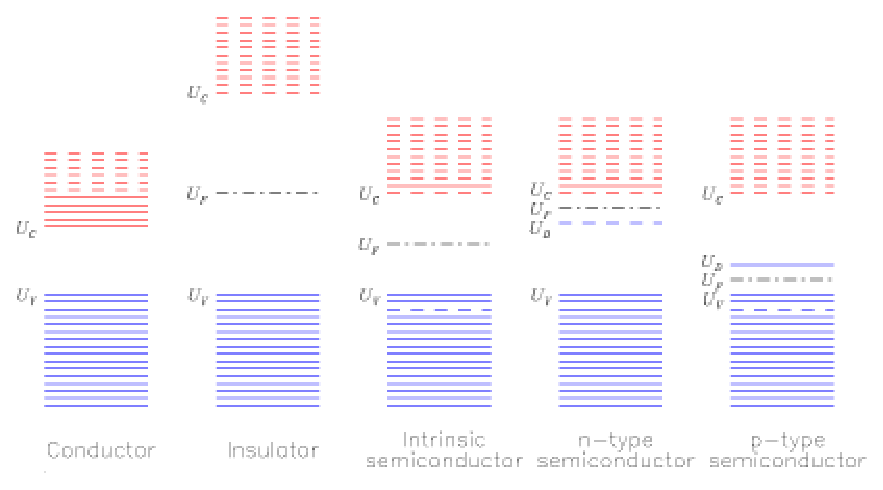
\includegraphics[width=0.95\textwidth]{CCD_solstate.eps}
	\caption{Solid state energy levels.}
	\label{fig:CCD.figsolstate}
\end{figure}

For crystalline silicon the corresponding energy gaps is 1.10 eV. In
this case some of the electrons may be thermally excited to the
conduction band even at room temperature. This leaves empty energy
levels (holes) in the valence band. This means that these materials
are semiconductors with an electrical conductance strongly dependent
on (and increasing with) the temperature of the material. Charge is
transported through the material not only by the thermally excited
electrons of the conduction band. An important observation is that
even an empty hole in an otherwise filled valence band will act as a
free positively charged, charge carrier. Neighboring electrons of the
valence band may under the influence of the imposed electric field
move into the empty electron state, resulting in the motion of the
hole in the opposite direction.

The number of electrons that are excited to the conduction band is
determined by the temperature through the Fermi-Dirac
distribution. The Fermi energy will vary in accordance with the number
of thermally excited electrons, typically taking values about halfway
between $U_V$ and $U_C$. This also means that if extra electrons are
added to the semiconductor, about half of these are added to the
conduction band, the other half occupying energy levels near the top
of the valence band that are made empty. A semiconductor that has an
equal number of holes and electrons that can move under the influence
of an electric field is called an intrinsic semiconductor. This type
of semiconductors stands in contrast to semiconductors contaminated
with foreign atoms.

In a silicon crystal contaminated with group V atoms (for instance
phosphor P), each foreign atom will replace one Si atom in the crystal
lattice and remain fixed in this location. The foreign atom
contributes one extra electron relative to the Si atom it replaces and
will therefore be called a donor atom. The extra electron will occupy
what are called donor impurity levels. In figure \ref{CCD.figsolstate}
these levels are denoted $U_D$. They are found just below the
conduction band, approximately 0.05 eV from the edge of the conduction
band. We recall that this is only twice the value of $\cl T$ at room
temperature. The electrons in the donor impurity levels are thus
easily thermally excited into the conduction band, leaving behind an
ionized donor atom in the lattice. Such materials conduct almost
entirely by negative charge carriers (electrons) and are called n-type
semiconductors. Under conditions of complete ionization the number
density of free charge carriers (electrons) will be equal to the
number density $N_D$ of impurity atoms.

If the silicon crystal instead is contaminated by group III atoms (for
instance boron B) each foreign atom will lack one electron for a
complete chemical binding. Such atoms will leave vacant levels (holes)
in the valence band. These atoms are therefore called acceptors.  The
vacant levels, called acceptor impurity levels and denoted $U_A$ in
figure \ref{CCD.figsolstate}, are located just above the top of the
valence band, approximately 0.05 eV from the edge of the valence band.
Neighboring valence band electrons are easily thermally excited into
the vacant levels where they will be trapped and not allowed to
move. They do, however, leave behind holes in the valence band which
may act as positive charge carriers. Such materials are therefore
called p-type semiconductors. Again the number density of free charge
carriers (holes) will be equal to the number density $N_A$ of impurity
atoms for a state of complete ionization.

We note that at low enough temperatures ($T < 70$ K) the ionization
degrees for both types of doped semiconductors become negligible and
therefore that the materials stop to act as semiconductors. This
phenomenon is referred to as ``freeze-out''. At this point the CCD
will cease to function.

\section{The photoelectric effect}

The photo-electric effect traditionally refers to a process in which
the energy $h\nu$ of a photon is absorbed by one electron in the
surface layer of a metal, and where the energized electron
subsequently escapes the metal with a maximum kinetic energy
\begin{equation}
  U_{kin} = h\nu - W.
\end{equation}
Here $W$ represents the work function of the metal, that is, the
energy needed to lift an electron from the top of the conduction band
to just outside the metal surface. The photo-electric effect is
important historically in that it clearly demonstrated the quantum
nature of light.

In the present context we are interested in the photo-electric effect
in doped semiconductors. The semiconductor will be initialized in a
completely depleted state, that is, every free charge carrier will be
driven away from the illuminated part of the material. We are
interested in the process where the photon energy $h\nu$ is absorbed
by a bounded, valence band electron, and where the electron is
lifted to the conduction band and therefore becoming a free charge
carrier in the semiconductor itself. The CCD detector relies on our 
ability to collect and subsequently count the number of such electrons
being produced.

The quantum efficiency for a CCD detector can be represented in the form
\begin{equation}
  QE = CCE(1-R_{ref}) \exp(-x_{poly}/L_A) (1-\exp(-x_{epi}/L_A))
  \label{CCD.QE}
\end{equation}
Here $CCE$ is the charge collection efficiency, that is, the ability
of the detector to collect all the photoelectrons generated. This is
often a factor of value close to unity. $R_{ref}$ is the reflection
coefficient for silicon at the wavelength of interest, and $L_A$ the
corresponding photon absorption length in the epitaxial layer of
effective thickness $x_{epi}$. The third factor in expression
(\ref{CCD.QE}) will be present for front side illuminated CCDs with
effective poly-crystalline gate thickness $x_{poly}$. 

\begin{figure}[h!]
%\hfil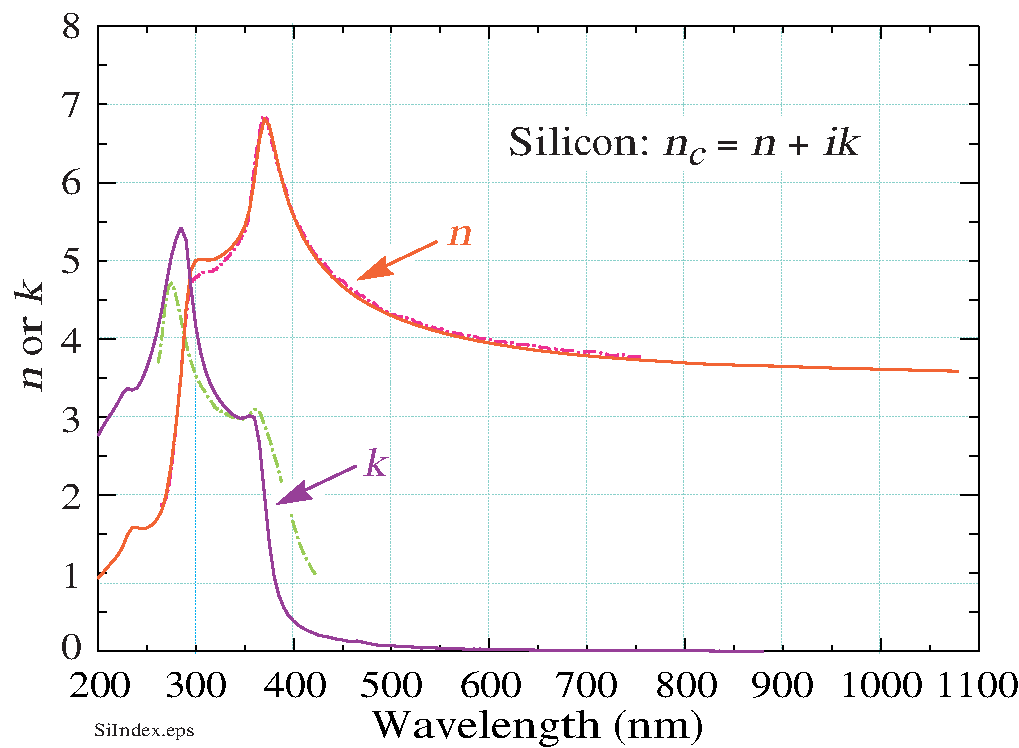
\psfig{file=SiIndex.eps,width=0.7\textwidth}\hfil
	\centering
	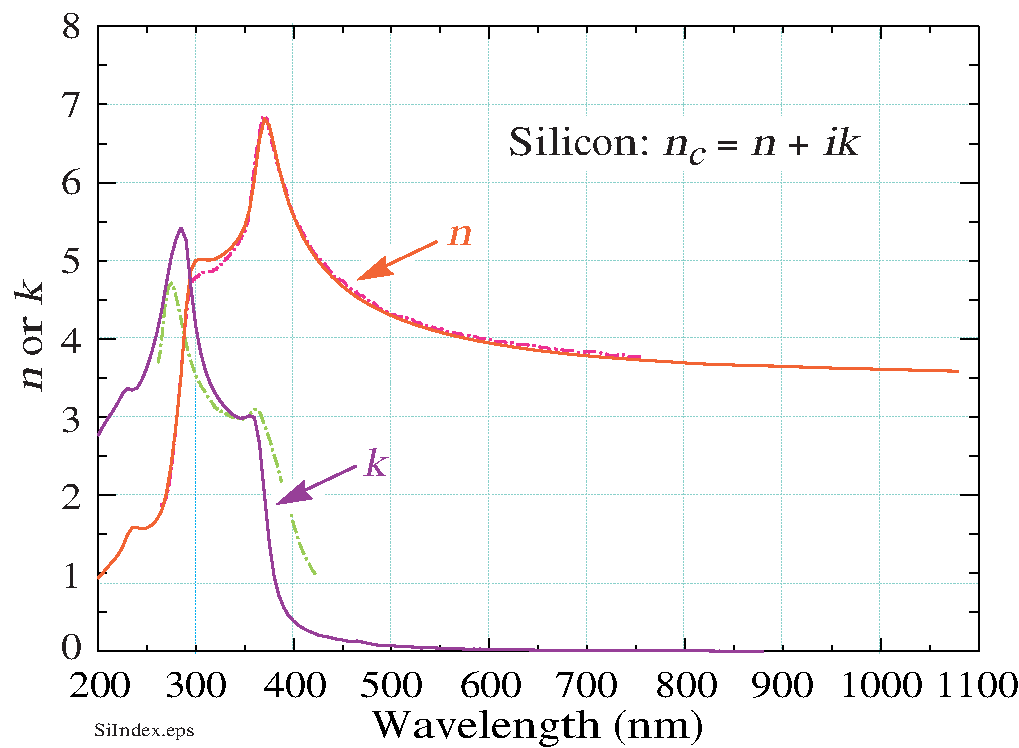
\includegraphics[width=0.7\textwidth]{SiIndex.eps}
	\caption{Reflection coeffecients (both real and imaginary) for Si as a function
		of wavelength.}
	\label{fig:si-refl}
\end{figure}

In figure~\ref{fig:si-refl} the reflection 
coefficient of silicon is plotted as a function of wavelength for the range 
200-1100~nm. In figure~\ref{fig:si-abs} the
corresponding absorption length is given for the same wavelength band.
We notice the reduced quantum efficiency in the UV to soft X-ray
range. Increased efficiency for wavelengths down to about 50~nm will
result by applying phosphor coatings to the illuminated side of the
CCD. The phosphor absorbs incoming photons of one wavelength and then
re-emits isotropically at a longer wavelength. A loss factor of 50~\%
results from the isotropic re-radiation property. A popular phosphor
is lumigen, effective for wavelengths less than 480~nm and
re-emitting at about 530~nm. 

\begin{figure}[h!]
%\hfil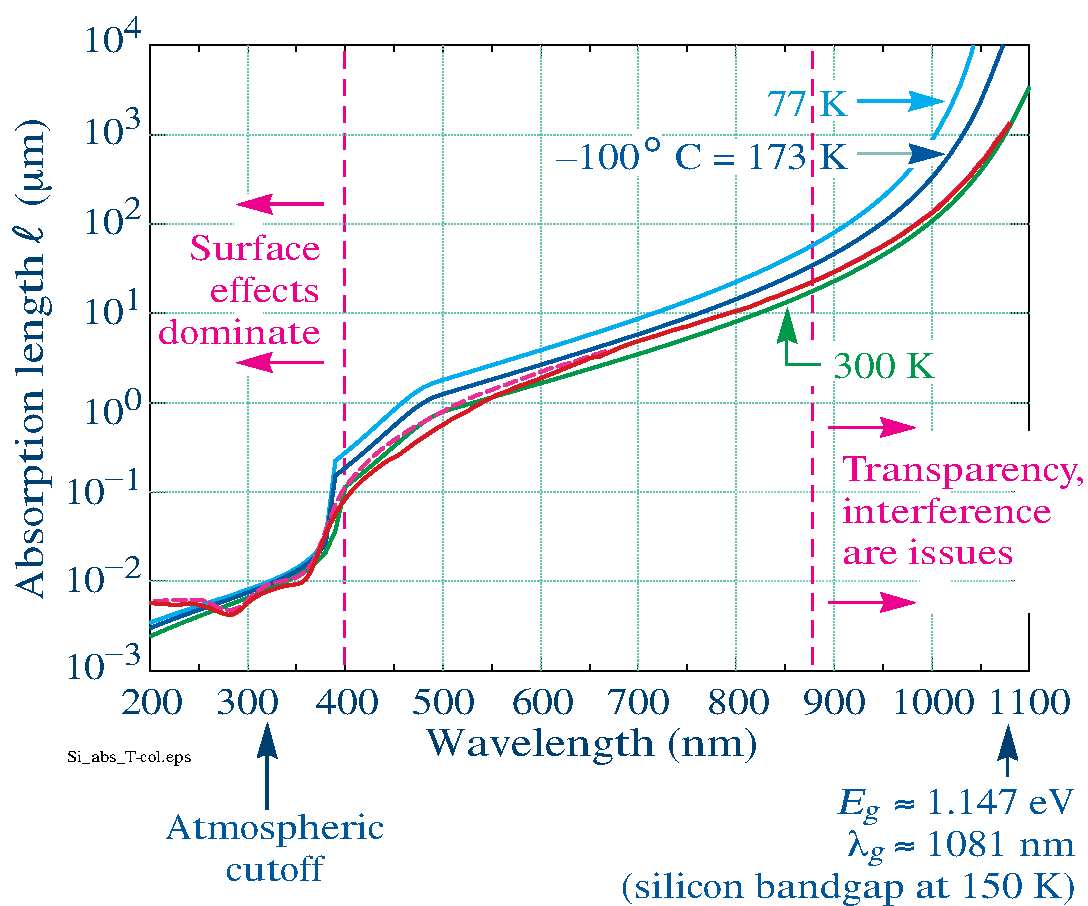
\psfig{file=Si_abs_T-col.eps,width=0.7\textwidth}\hfil
	\centering
	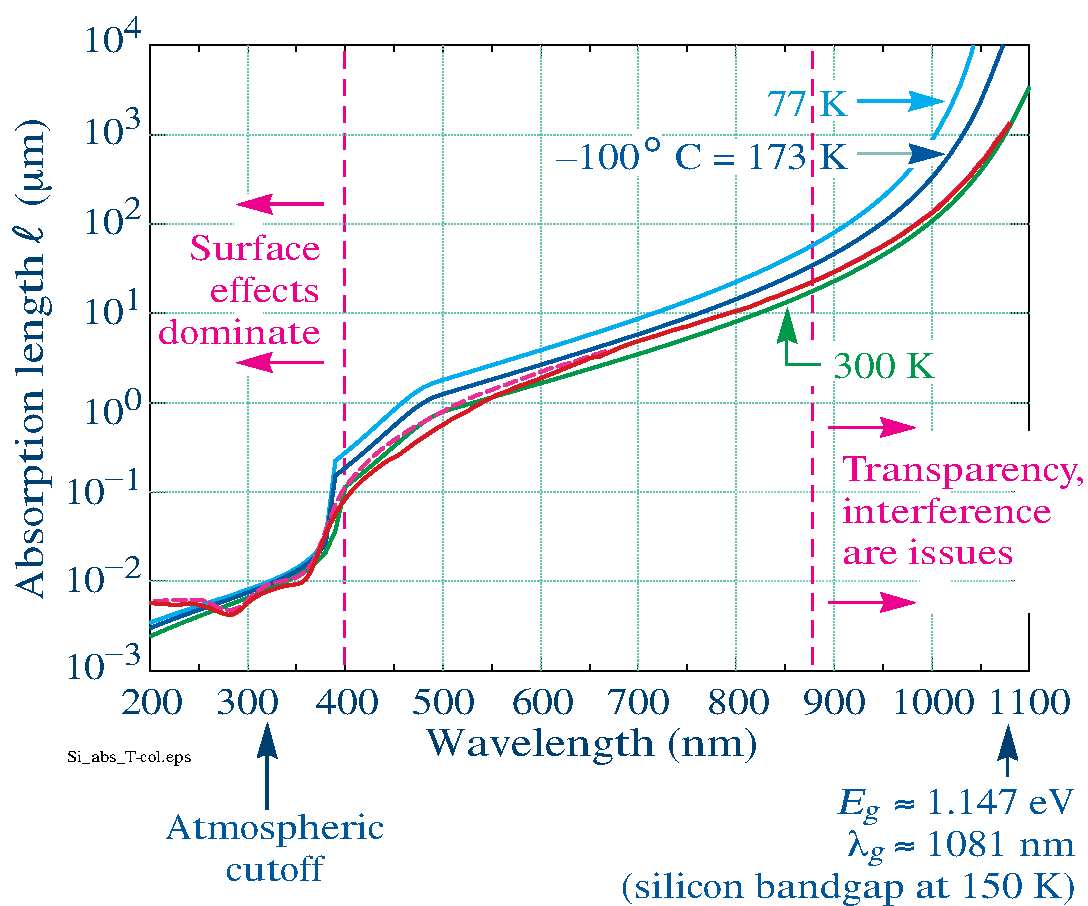
\includegraphics[width=0.7\textwidth]{Si_abs_T-col.eps}
	\caption{Absorption length of Si as a function of wavelength and temperature.}
	\label{fig:si-abs}
\end{figure}

To be able to lift a valence-band electron to the conduction band the
photon energy $h\nu$ must exceed the band gap energy, $U_C-U_V \approx
1.1$ eV for silicon. This corresponds to wavelengths $\lambda < 1090$~nm. 
For photons with less energy silicon will appear transparent. Note in 
connection with this that the electrodes at or near the surface of a
detector such as a CCD can reflect some of the incident light thus reducing
the detectors efficiency. One solution to this is to replace 
metallic electrodes with transparent polysilicon electrodes. Alternately,
the detector may be illuminated from the back so that it does not have to
pass through the electrodes at all. This, though, requires that the silicon
forming the detector be very thin so that the electrons produced by 
incident radiation are collected efficiently. This process is difficult
and many devices may be damaged during operation. Successfully thinned
CCDs are therefore expensive as well as being fragile. At longer 
wavelengths the thinned CCD can become semi-transparent, this reduces the
efficiency of the CCD and may in addition cause interference fringes 
to be produced, which must be removed in the data reduction process. Both
of these effects are visible in figure~\ref{fig:crisp8542raw-momfbd}, which
features a solar image taken in the infrared 854.2~nm Ca~{\sc ii} line.

\begin{figure}[p]
	\centering
%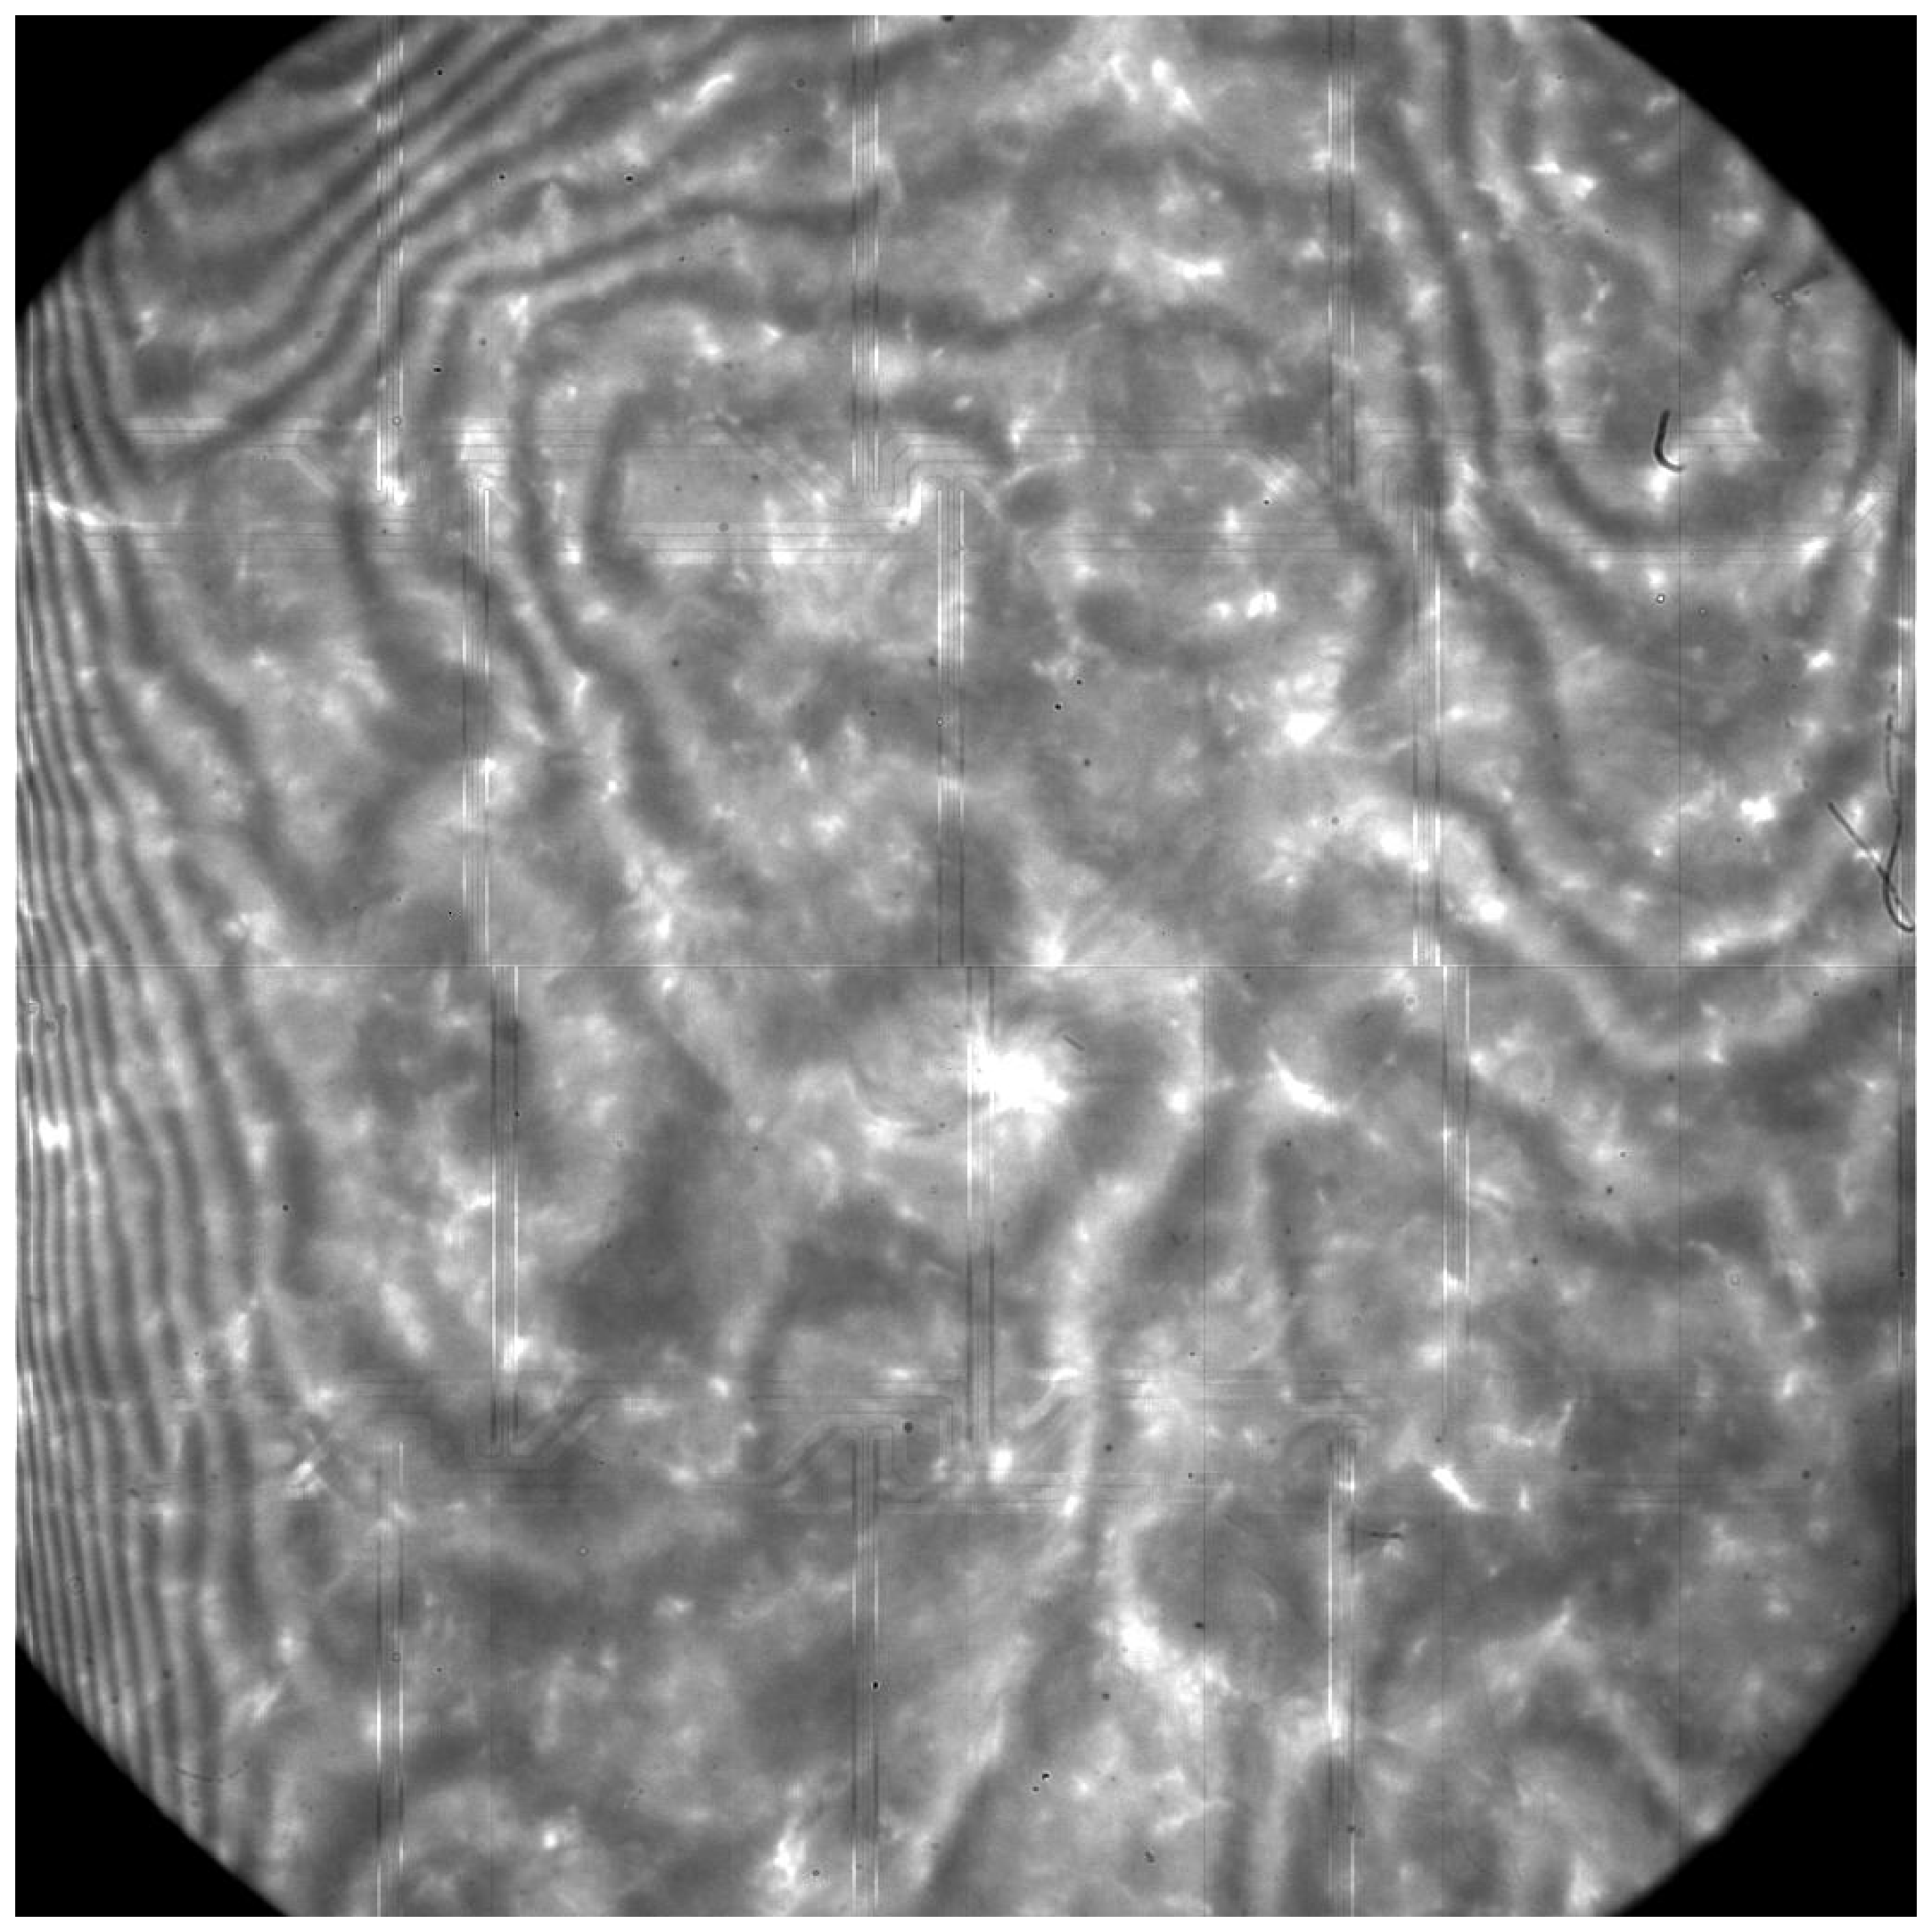
\psfig{file=camXXV_13Jun2008_8542_raw.eps,width=0.7\textwidth}
%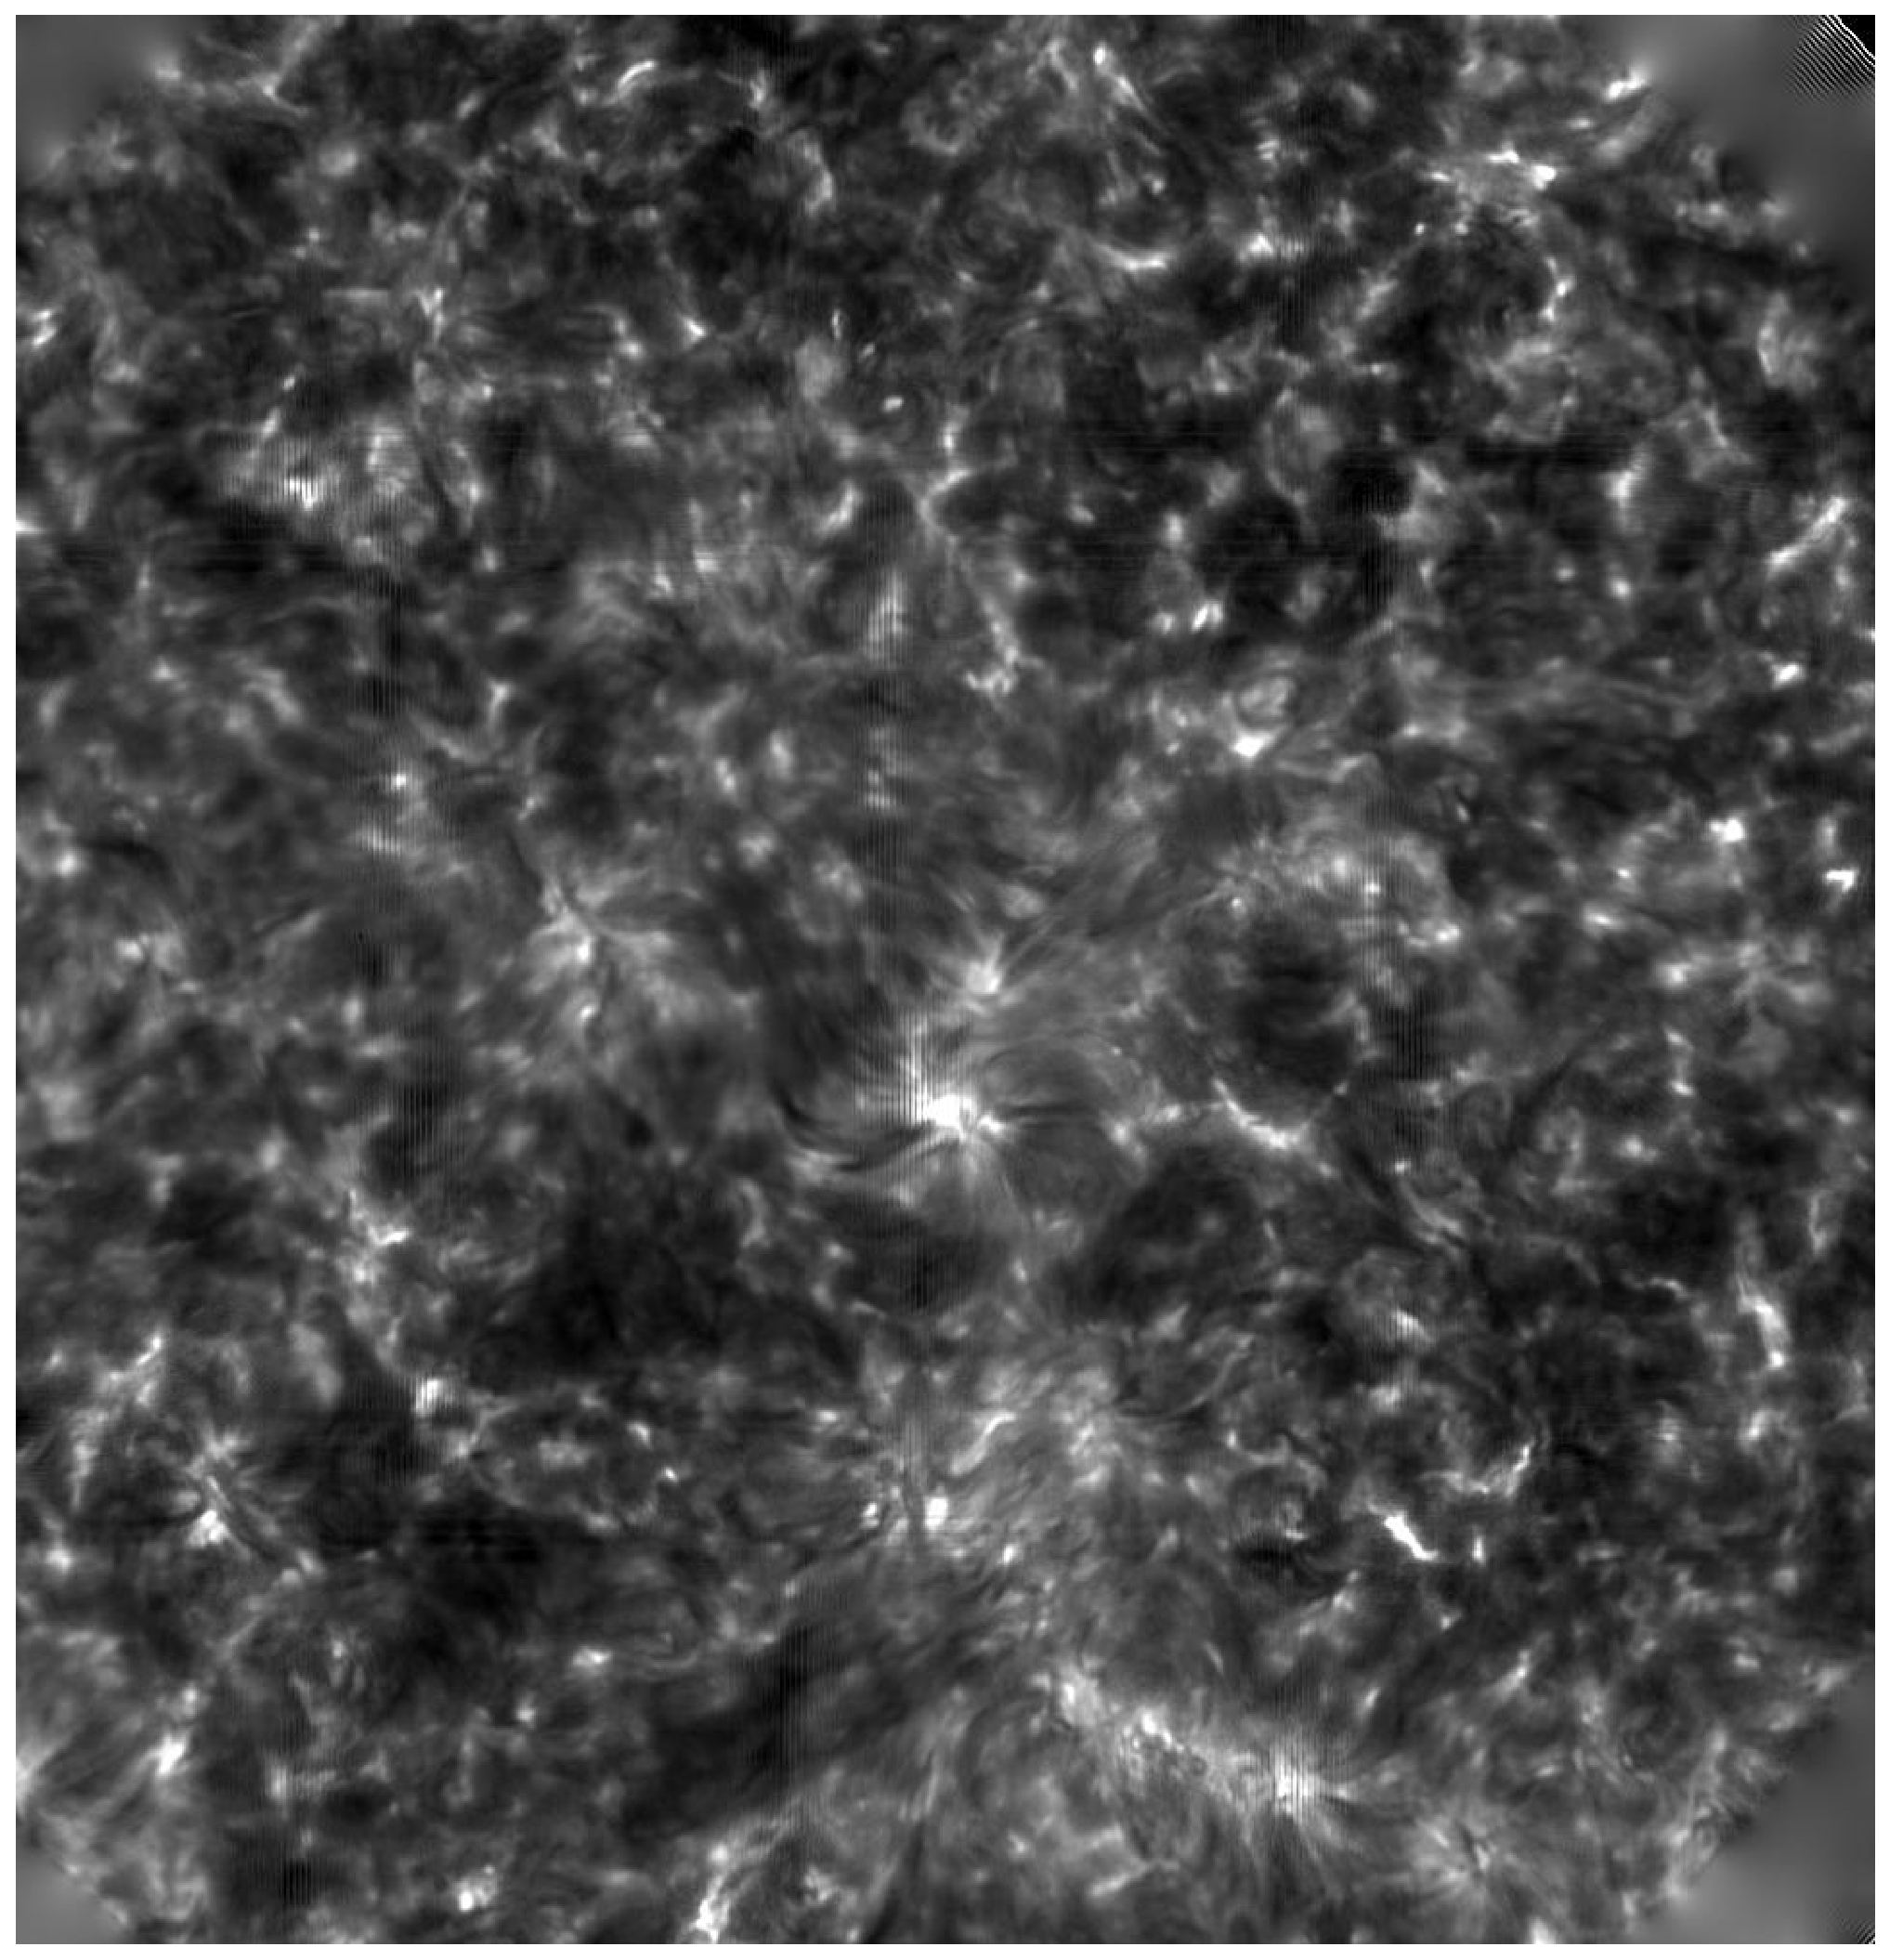
\psfig{file=camXXV_13Jun2008_8542_momfbd.eps,width=0.7\textwidth}}
		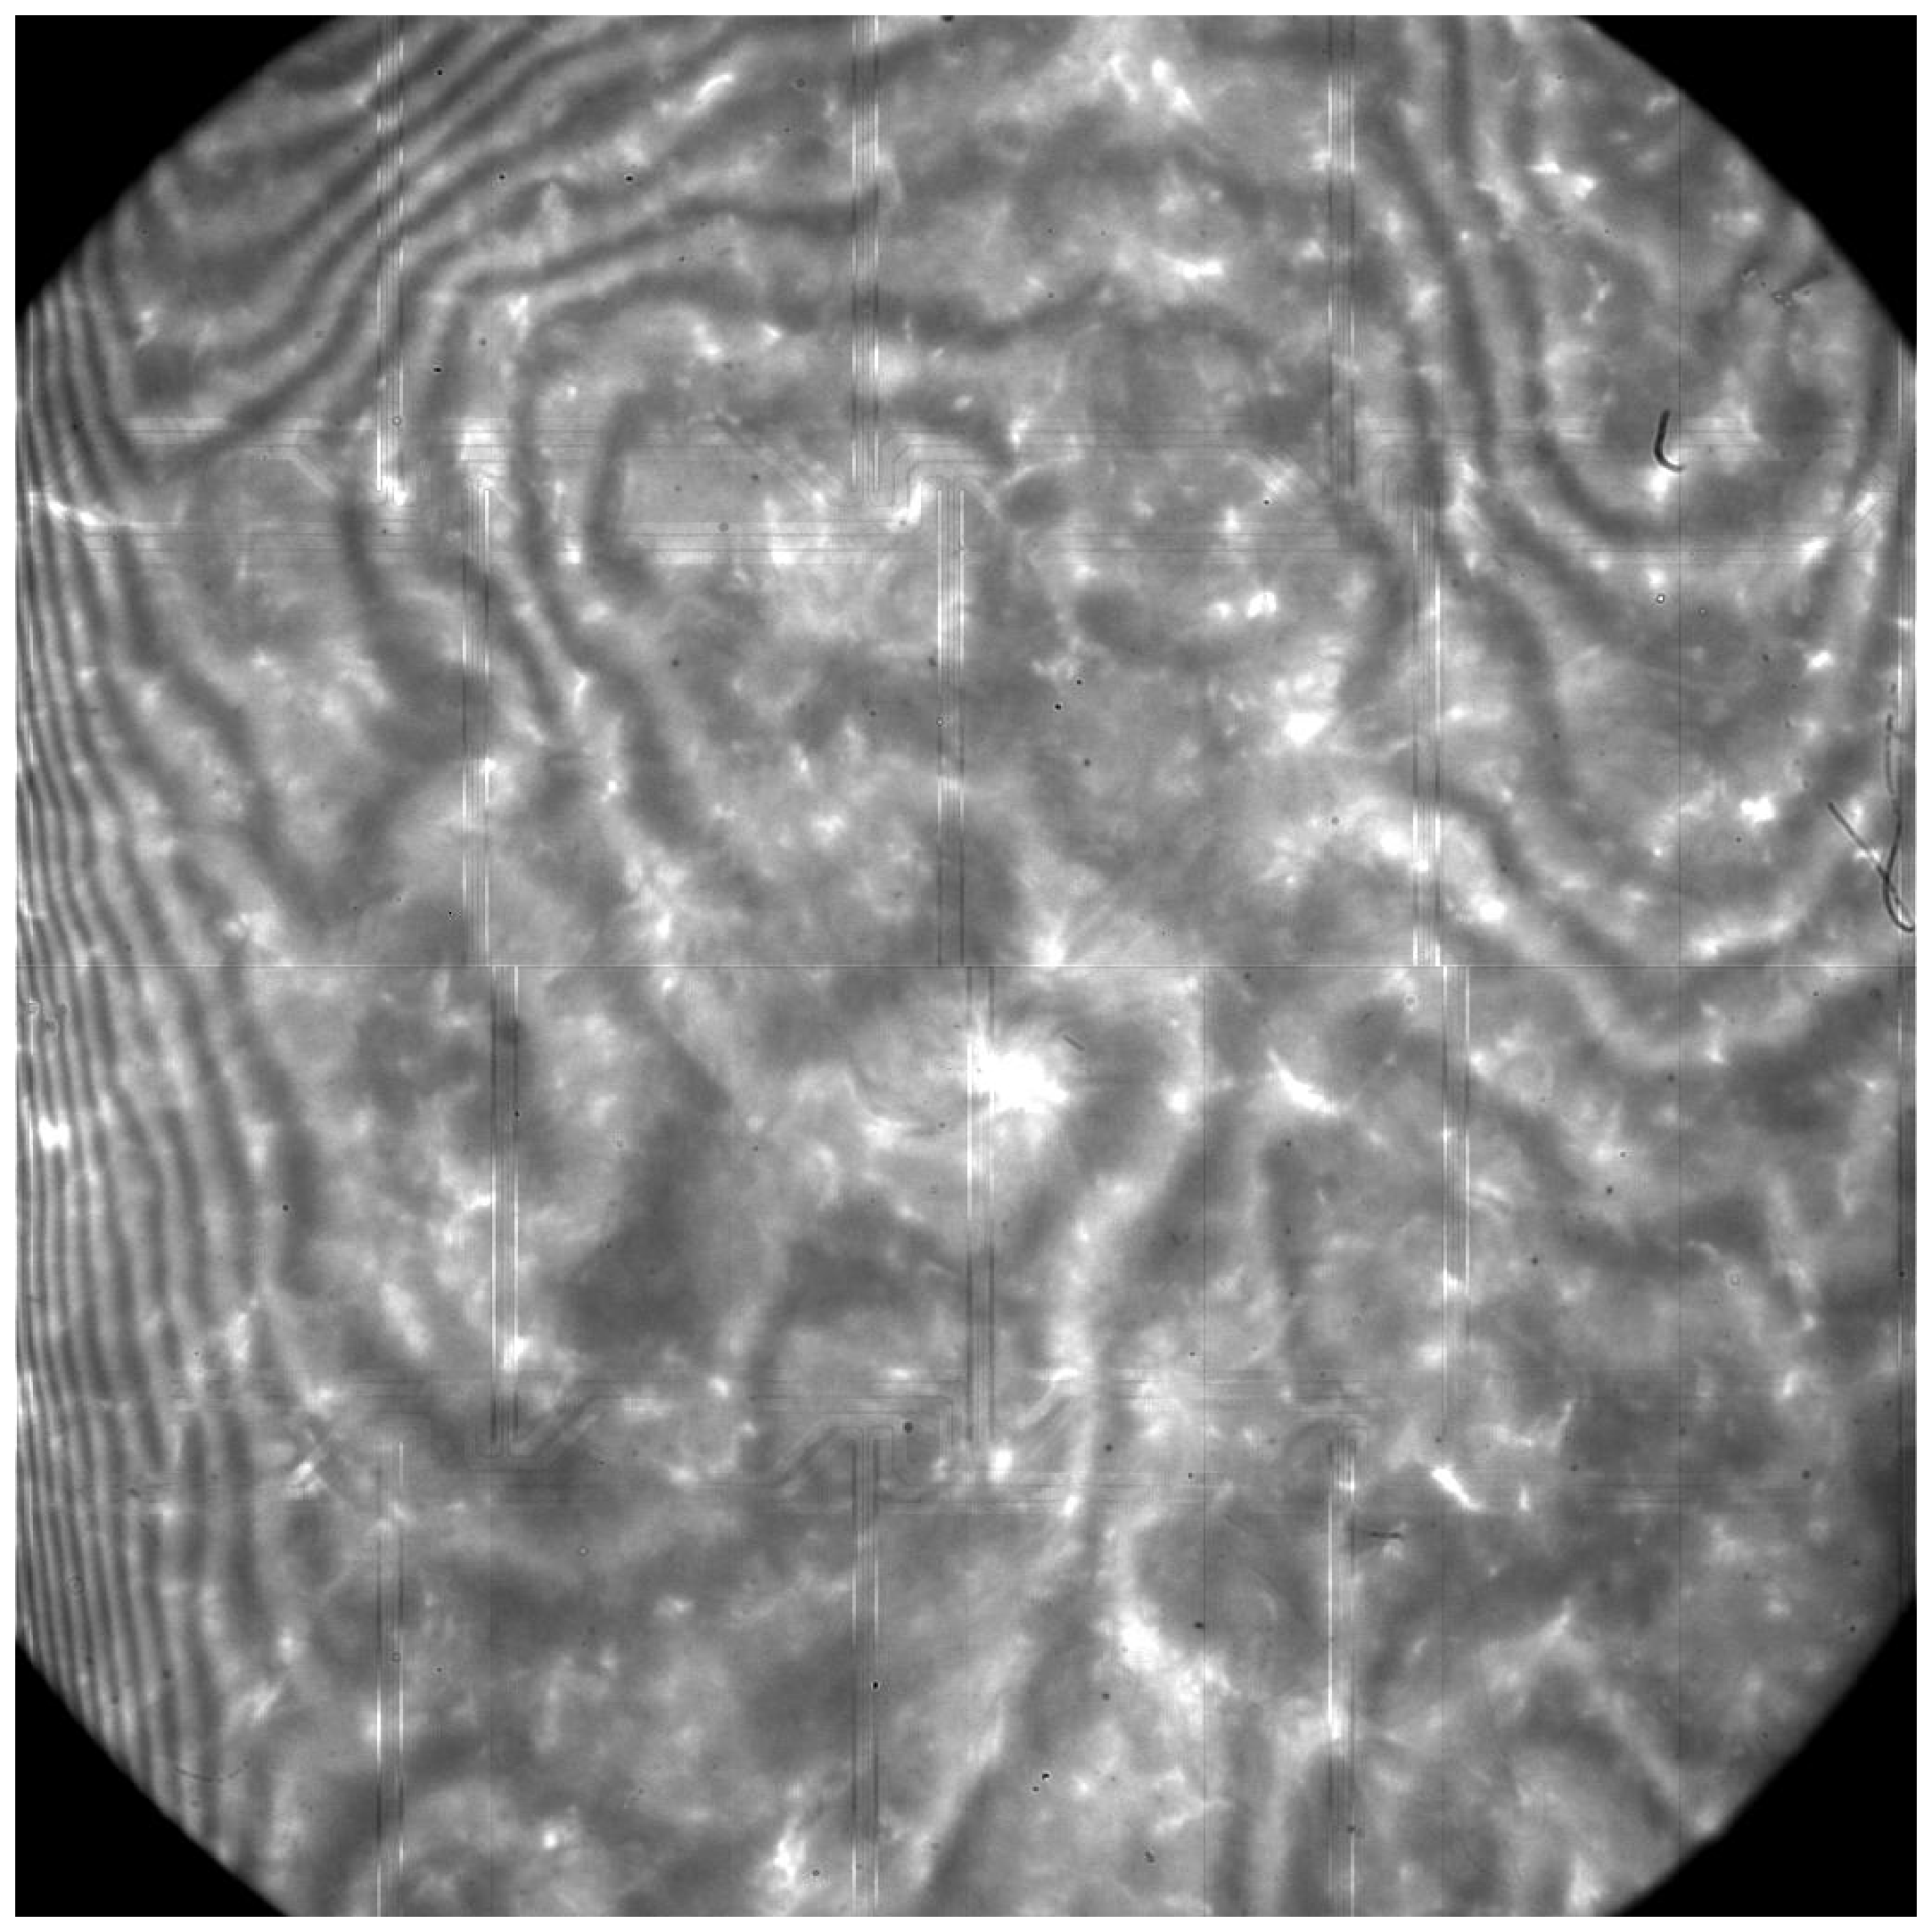
\includegraphics[width=0.7\textwidth]{camXXV_13Jun2008_8542_raw.eps}
		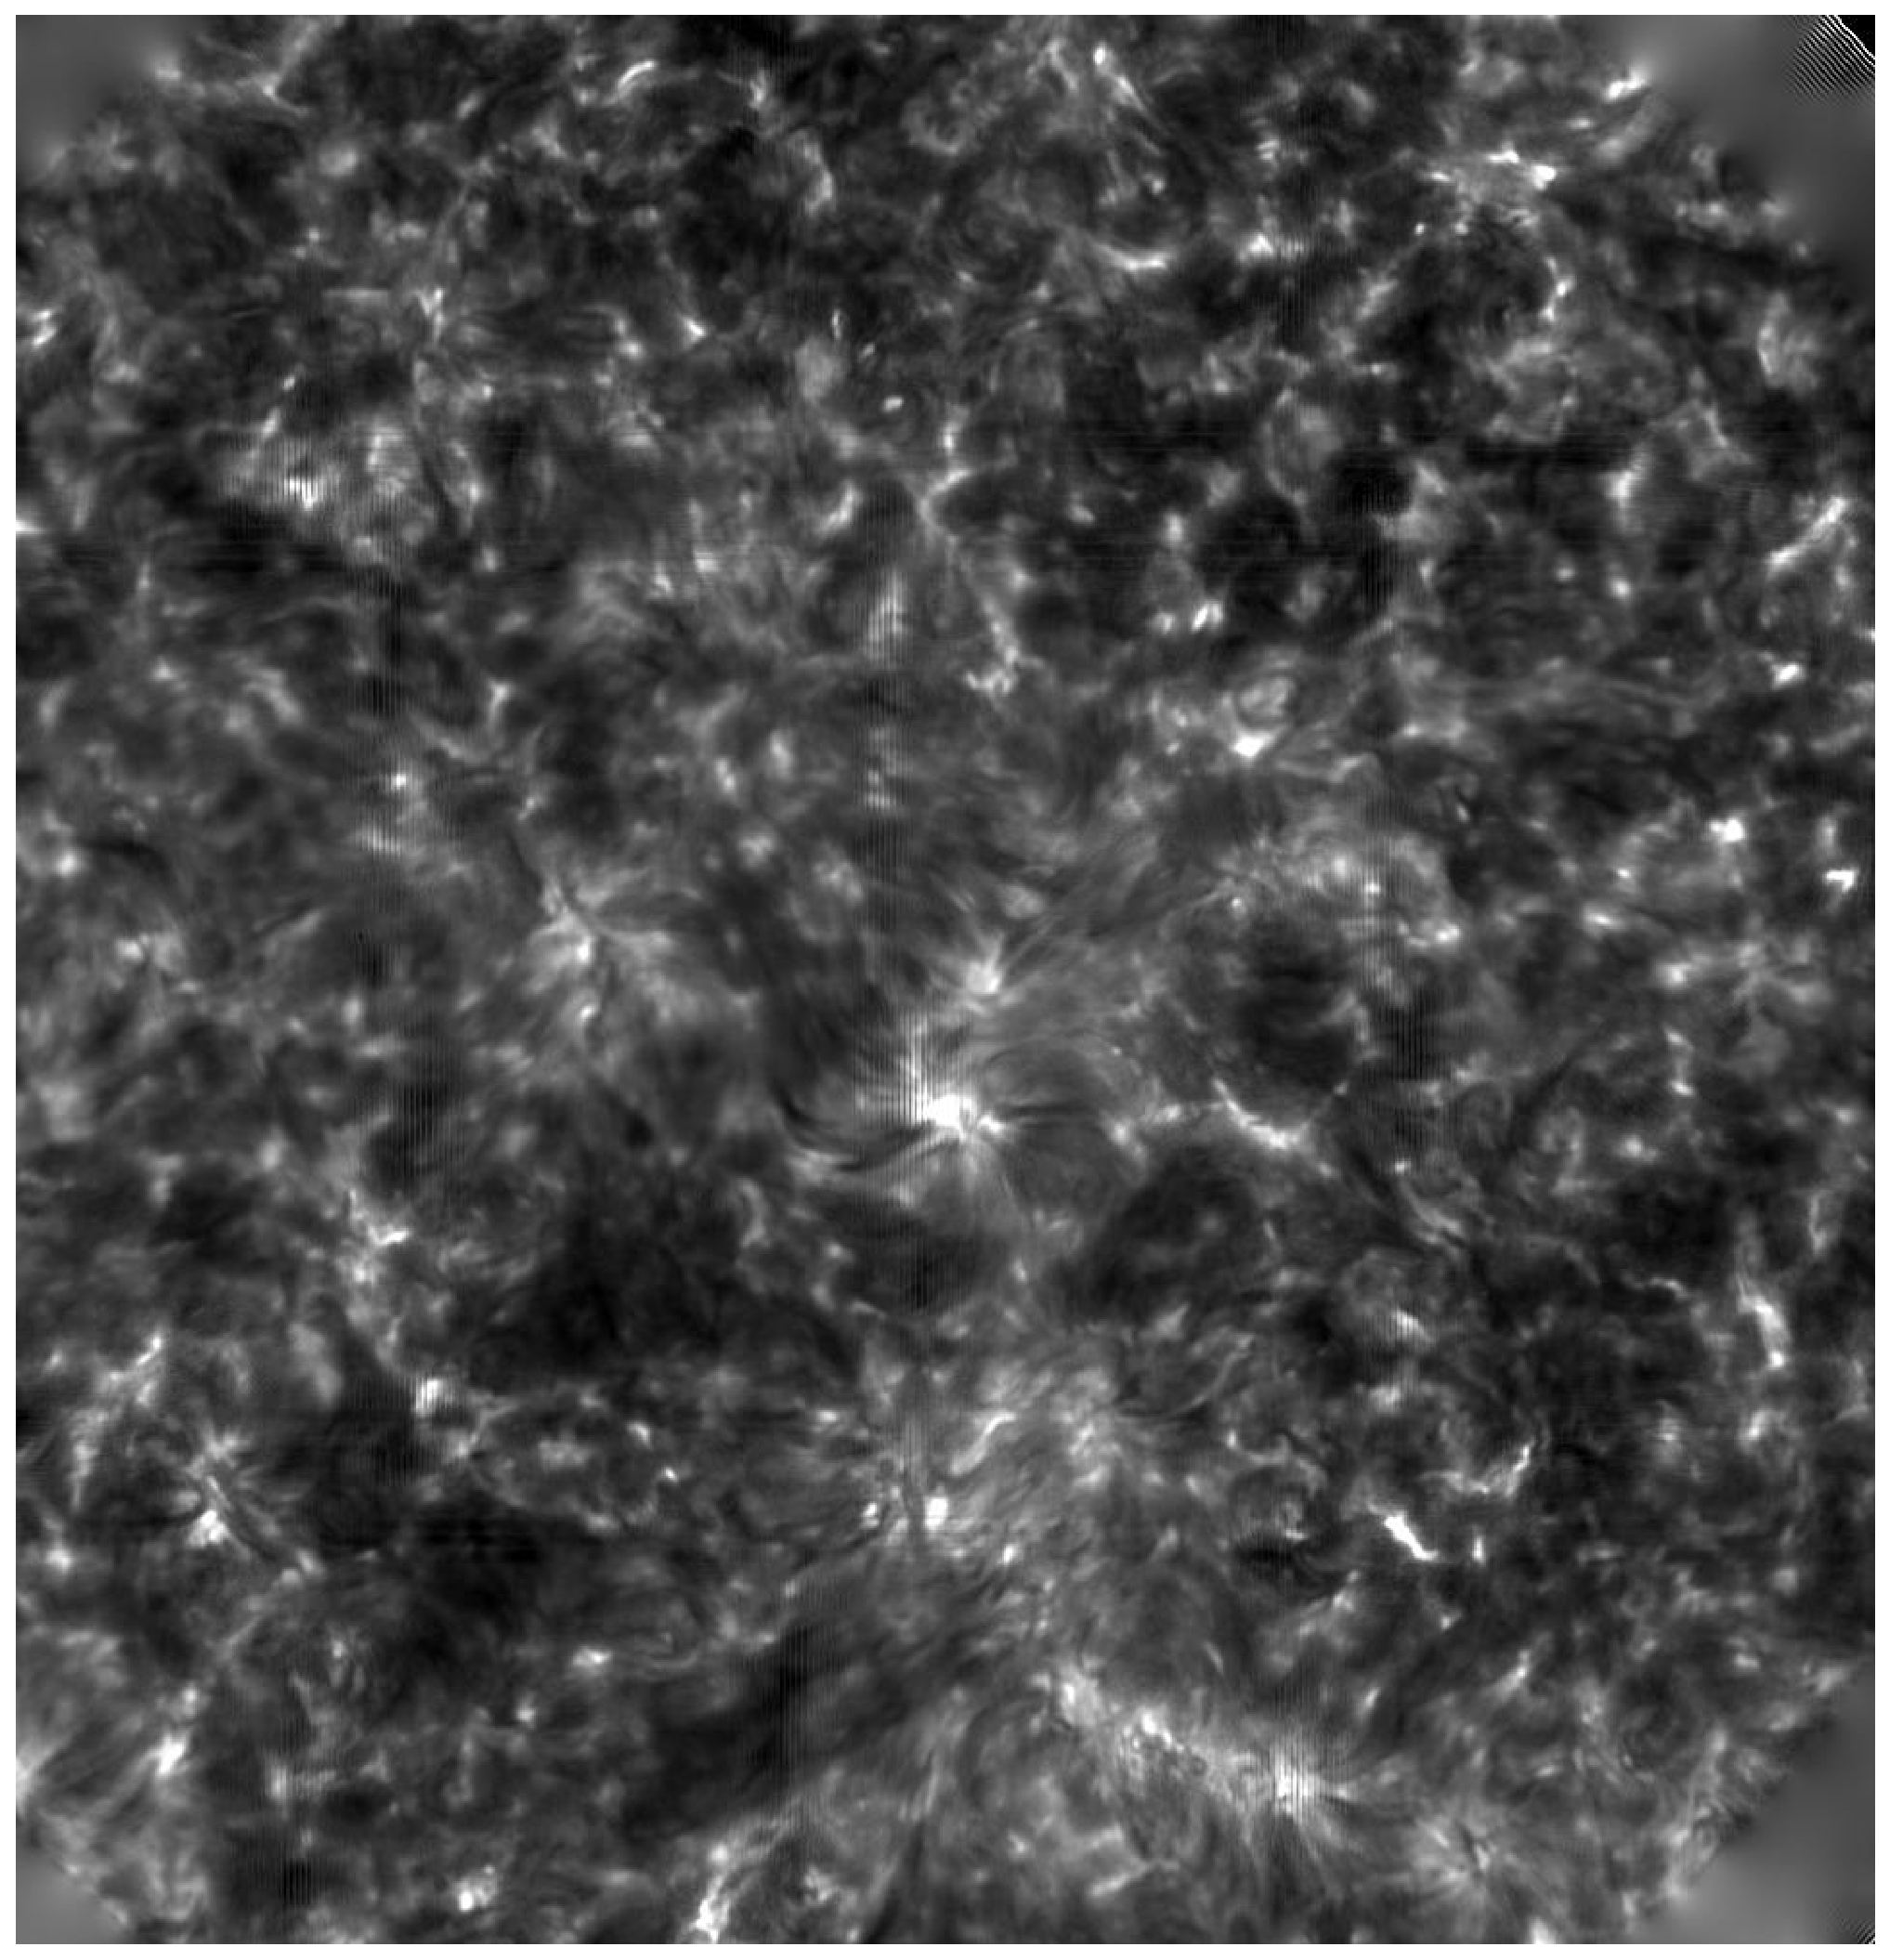
\includegraphics[width=0.7\textwidth]{camXXV_13Jun2008_8542_momfbd.eps}
	\caption{Pre- and post-processed images taken of the quiet Sun in the 
	$\lambda 8542$~\AA\ line of Ca~{\sc ii} at the Swedish 1-meter Solar 
	Telescope, June 13, 2008 with the CRISP Fabry-Perot focal plane instrument. 
	Notice that at this wavelength the CCD is partly transparent.
	Notice also the patterns due fringing. Most, if not all, of these
	artifacts can be removed with {\it e.g.} MOMFBD techniques.}
	\label{fig:crisp8542raw-momfbd}
\end{figure}
% example from SST!

For photon energy in the range 1.14 to 3.1~eV a single electron-hole pair
is produced. At higher energies multiple electron-hole pairs will be
produced by a single photon as energetic conduction band electrons
collide with other valence band electrons. The average number of
conduction band electrons effectively generated for photon energy
$h\nu > 10$~eV is approximated by the empirical formula
\begin{equation}
  \eta = h\nu/E_{e-h}
\end{equation}
where $E_{e-h} \approx 3.65$~eV for silicon.

\section{CCDs}

The CCD-detector (Charge-Coupled Device) was invented in 1969 by Boyle
and Smith at Bell Telephone Laboratory, the same laboratory where the
transistor was invented 20 years earlier. The CCD was originally
intended for use as computer memory. Its usefulness as a
electromagnetic radiation detector was, however, discovered only a few
years later. The first application of a 400$\times$400$\times 15~\mu$m
pixel CCD for high-resolution astronomical imaging was made in
1975. Since then the CCD has developed into becoming the major image
forming detector for infrared, optical and X-ray wavelengths in
astronomy as well as in other fields.  Examples include the original
800$\times$800$\times 15~\mu$m pixel detectors for the (three-phase)
Wide Field Planetary Camera (WF/PC) of the Hubble Space Telescope or
the (virtual phase) 1024$\times$1024$\times 18~\mu$m pixel detector
for the Solar X-ray Telescope of the Yohkoh Satellite. CCD detectors
are presently routinely produced in sizes 2k$\times$4k pixels, but
have also been produced in sizes up to 10000$\times$10000
pixels. Detectors of this size or larger are becoming impractical due
to rapidly increasing read-out times and production costs.

\section{A simplified three-phase CCD lay-out}

The CCD depends for its functioning as a photon counting device on
four different operations: 1) the conversion of individual photons to
elementary electric charges during the illumination period, 2) the
storing of these charges over the desired exposure time, 3) the
transfer of the stored charges from pixel to pixel for the read-out
procedure, and finally 4) the accurate read-out of the accumulated
charge for each pixel element.  

In figure \ref{CCD.figschematic} a schematic lay-out for a three-phase
4$\times $5 CCD detector matrix is illustrated.  On top of a strongly
doped p-type silicon substrate is laid a weakly doped p-type epitaxial
layer, a subsequent electrically insulating SiO$_2$ layer and finally
a layer of individual transparent, poly-crystalline silicon gate
electrodes.  Each pixel element consists of three such electrodes
connected to three clocking voltage generators A, B and C. The colored
region represent the size of one pixel. Each line of pixels is
electrically separated from the neighboring lines by a strongly doped
p-implant under the oxide layer, indicated by blue lines in the
figure. The electrodes A, B and C for each pixel are electrically
connected to the similar electrode of the other pixels. In addition to
the 4$\times$5 pixel matrix the figure shows a 4 element register with
a separate set of A, B and C electrodes. The register which is
shielded from radiation is needed for the read-out process.

\begin{figure}[h]
  \centering
	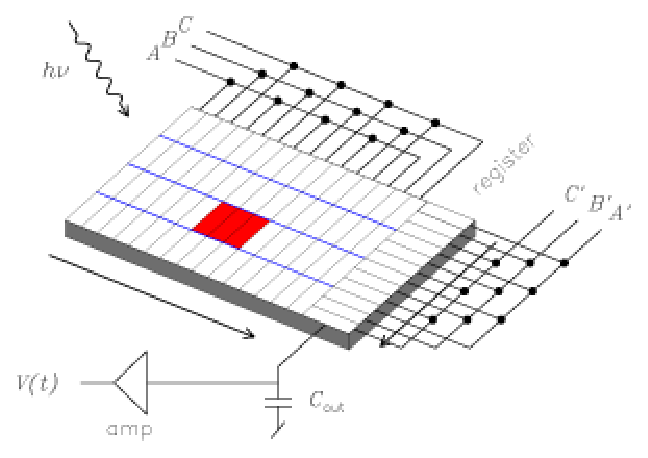
\includegraphics{CCD_schematic.eps}
  \caption{Schematic lay-out of a three-phase CCD detector}
  \label{CCD.figschematic}
\end{figure}

1) During the illumination phase the B-gate is held at high potential
(10 V) while the A- and C-gates are kept at low potential (2
V). Individual photons penetrating into the p-layer excites valence
band electrons into the conduction band. 

2) These electrons are collected in the potential well created under
the B-gate. The low potential of the A- and C-gates isolates charges
generated in any given pixel element from those generated in the
neighboring pixels.

3) The charge transfer phase is initiated by lifting C-gate to high
potential. This widens the trapping potential well and drives the
accumulated electrons towards the C-gate. This charge transport is
strengthened by subsequently lowering the potential at the B-gate. The
accumulated electrons are by now transported from under the B-gate to
under the C-gate. This procedure is next repeated twice, transporting
the electrons further on to the A- and B-gates of the subsequent pixel
element. The full procedure is then repeated until the charges
accumulated over the full length of the detector array have been
shifted out at the far end.

4) At the far end the individual shifted charge packets are dumped into
the register. Before the next set of charge packets from the different
pixels lines can be dumped to the register, the contents of the
register cells are shifted out to the measuring capacitor $C_{out}$ and
recorded by a charge measuring circuit. From the recorded
charge-versus-time series, the originating pixel element for each
charge packet can be identified and the recorded image reconstructed.

We will return to study different aspects of these different stages of
the CCD detector in greater detail below.

\subsection{Other types of clocking}

Astronomical CCDs are mainly three phase devices, but there are other types
as well. 

A two phase CCD requires only a single clock, but needs double electrodes 
to provide directionality to the charge transfer process. Each pixel consistes
of two electrodes, one located deeper into the substrate than the other, 
linked to the same voltage source. Every other pixel is connected to 
alternating voltage sources. When the voltages cycle between, say, 2~V and
10~V the stored charge is attracted over to the nearer of the two neighboring
surface electrodes and then accumulates again under the buried electrode.

Virtual phase CCDs require only one set of electrodes. Additional wells with
a fixed potential are produced by p and n implants directly into the silicon
substrate. The active electrode can then be at higher and lower potentials 
as required to move the charge through the device. The active electrodes
in a virtual phase CCD are physically separated from each other leaving 
parts of the substrate directly exposed to incoming radiation. This 
enhances their sensitivity.

\section{The surface channel MOS capacitor}

Let us now consider the particular silicon structure illustrated in
figure \ref{CCD.figpMOS}. On top of a heavily doped p-substrate
another weakly doped (epitaxial) p-layer with acceptor density $N_A$
is laid, then a layer of SiO$_2$ and finally a layer of
poly-crystalline silicon. The latter two layers act as an insulator and
a conductor, respectively. Note that the conducting poly-layer has
been broken up into three separate parts for each pixel for reasons to
be explained below. The dielectric constants (permitivities) of the
oxide and p-layers are $\epsilon_{ox} = 3.45 \times 10^{-11}$ F/m and
$\epsilon_{si} = 1.04\times 10^{-10}$ F/m, respectively.  The oxide
layer will prevent conduction currents to cross. The structure can
therefore be characterized as a metal-oxide-semiconductor (MOS)
capacitor.

\begin{figure}[h]
  \centering
	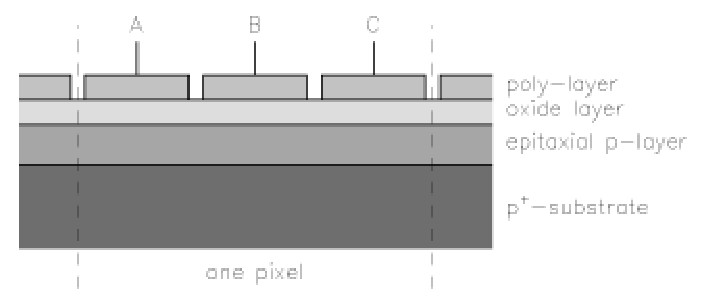
\includegraphics{CCD_pMOS.eps}
  \caption{Surface channel MOS capacitor}
  \label{CCD.figpMOS}
\end{figure}

Let the top conductive layer be given a few volts positive bias
relative to the substrate. Due to the bias voltage $V_G$ an electric
field will be established across the insulator layer and reaching a
distance $x_d$ inside the p-layer. Within this distance holes will be
swept away, leaving a region depleted of free charge carriers but with
space charge density $-e N_A$ due to the fixed acceptor ions. The
insulating layer and the depleted part of the p-layer act as two plane
parallel capacitors in series, with capacitances
\begin{equation}
  C_{ox} = \frac{\epsilon_{ox}}{d}
  \quad {\rm and} \quad C_{dep} = \frac{\epsilon_{si}}{x_d}.
\end{equation}
Inside the oxide layer a constant electric field $E_{ox}$ will be
established. Due to the existing space charge density the potential
inside the depletion region will satisfy the Poisson equation
\begin{equation}
  \dd{V}{x} = \frac{e N_A}{\epsilon_{si}}
\end{equation}
with solution
\begin{equation}
  V(x) = \frac{e N_A}{2\epsilon_{si}} (x-x_d)^2.
\end{equation}
The electric field at the oxide-silicon interface at $x=0$ is thus
given by
\begin{equation}
  E_S = -{dV\over dx}(x=0) = \frac{e N_A x_d}{\epsilon_{si}}.
\end{equation}
The discontinuity in the dielectric constant at this interface means
that there will exist a corresponding discontinuity in the electric
field. Thus (remembering that $\nabla\cdot(\epsilon{\bf E})=\rho_{free}$) 
inside the oxide layer the electric field is related to
$E_S$ through
\begin{equation}
  \epsilon_{si} E_S - \epsilon_{ox} E_{ox} = 0.
  \label{CCD.divD}
\end{equation}
The total voltage drop over the two capacitors can now be expressed in
the form
\begin{equation}
  V_G = E_{ox}d + \frac{e N_A}{2\epsilon_{si}} x_d^2,
  \label{CCD.surVG}
\end{equation}
from which an explicit expression for the thickness $x_d$ of the
depletion layer follows,
\begin{equation}
  x_d = -\frac{\epsilon_{si}}{C_{ox}} +
  \sqrt{\left(\frac{\epsilon_{si}}{C_{ox}}\right)^2
       +\frac{2\epsilon_{si}}{eN_A}\, V_G}.
  \label{CCD.xd}
\end{equation}
The result is plotted in figure \ref{CCD.figsurchan} for different
gate voltages $V_G$ for a case with uniform acceptor density $N_A =
1\times10^{21}$ m$^{-3}$.

\begin{figure}[h]
  \centering
	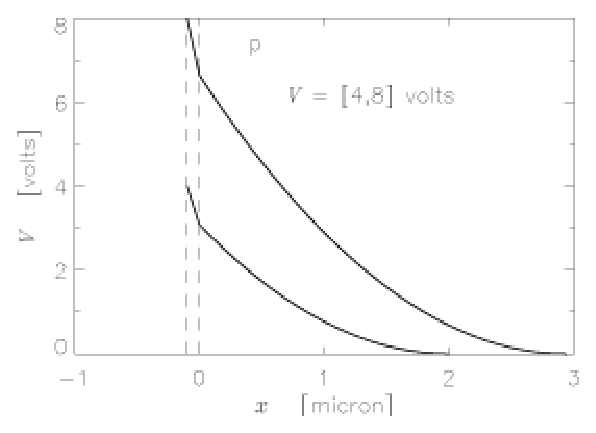
\includegraphics{CCD_surchan.eps}
  \caption{Surface channel potential well.}
  \label{CCD.figsurchan}
\end{figure}

If the depletion layer is now illuminated, electron-hole pairs may be
formed. Under the influence of the existing electric field in this
region the holes will drift to the right in figure
\ref{CCD.figsurchan}. The electrons go to the left and are trapped in
the potential well at the oxide-silicon interface. If at a given time
$\tau$ during the illumination $\cl N$ electrons per unit interface
area are collected, then these represent a negative surface charge
density $\cl Q = -e\cl N$. With this surface charge present the
relation (\ref{CCD.divD}) between the electric field in the oxide layer
and the surface electric field in the depletion region must be
replaced by
\begin{equation}
  \epsilon_{si} E_S - \epsilon_{ox} E_{ox} = \cl Q
\end{equation}
When substituted in (\ref{CCD.surVG}) this means that the expression
for the thickness of the depletion region (\ref{CCD.xd}) is
transformed into
\begin{equation}
  x_d = -\frac{\epsilon_{si}}{C_{ox}} +
  \sqrt{\left(\frac{\epsilon_{si}}{C_{ox}}\right)^2+\frac{2\epsilon_{si}}{eN_A} \, V_Q},
\end{equation}
with
\begin{equation}
  V_Q = V_G + \frac{\cl Q}{C_{ox}}.
\end{equation}
Obviously, the holding capacity of the MOS capacitor for a given gate
voltage $V_G$ is exceeded when $x_d \rightarrow 0$.

\section{The buried channel MOS capacitor}

The surface channel MOS capacitor studied above met with serious
difficulties in practical applications. A fraction of the accumulated
electrons tended to get trapped at imperfections at the oxide-silicon
interface. It was thus not possible to achieve the CTE values required
to build large array CCD detectors. Thus, the buried channel MOS
capacitor was invented. This structure, showing remarkable CTE
performance, differ from the corresponding surface channel structure
by having an extra n-layer (donor density $N_D$) of thickness $t$
introduced between the oxide and p-layer. The structure is
illustrated in figure~\ref{CCD.fignMOS}.

\begin{figure}[h]
  \centering
	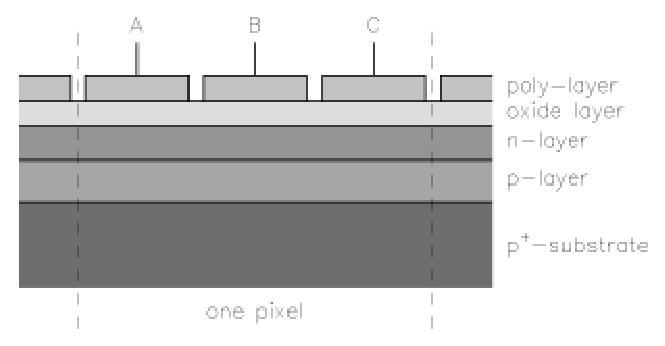
\includegraphics{CCD_nMOS.eps}
  \caption{Buried channel MOS capacitor}
  \label{CCD.fignMOS}
\end{figure}

The analysis of the buried channel MOS capacitor is only slightly more
complicated than the preceding one. The extra n-layer reshapes the
potential well to form a potential maximum between the oxide-silicon
interface and the new n-p junction. To perform as a photo-detector,
however, it is of major importance to make sure that complete
depletion of majority carriers (electrons) in the n-layer has been
achieved before the photon counting sequence is initiated. We return
to a discussion of this requirement below.

\subsection{Potential well}

If we for the time being assume the depletion condition to be
satisfied the shape of the potential well is found by solving the
Poisson equation in the form
\begin{equation}
  \dd{V}{x} = \left\{ \begin{array}{ll} 
	0 & -d < x < 0 \\
	\frac{\displaystyle -eN_D}{\displaystyle \epsilon_{si}} \quad &
	0 < x < t \\
	\frac{\displaystyle eN_A}{\displaystyle\epsilon_{si}} & 
	t < x < t+x_p \\
	0 & t+x_p < x
  \end{array} \right.
  \label{CCD.Poissonbur}
\end{equation}
where $x_p$ now denotes the thickness of the p-layer depletion
region. The boundary conditions require the potential to be a
continuous function for the full $x$-range. The same applies for the
electric field $E = -\rd V/\rd x$, except at the oxide-silicon
interface where a discontinuity in the dielectric constant exits.
The solution is
\begin{equation}
  V(x) = \left\{ \begin{array}{ll} 
	V_G-E_{ox}(x+d) & -d < x < 0 \\
	V_{max} - \frac{\displaystyle
	eN_D}{\displaystyle 2\epsilon_{si}} (x-t+x_n)^2 \quad & 
	0 < x < t \\ 
	\frac{\displaystyle eN_A}{\displaystyle
	2\epsilon_{si}}(x-t-x_p)^2 & t < x < t+x_p \\
	0 & t+x_p < x 
	\end{array} \right.
  \label{CCD.bursol}
\end{equation}
where $V_{max}$ is the potential maximum occurring at a distance $x_n$
from the n-p junction. With the chosen form (\ref{CCD.bursol}) of the
solution the boundary conditions at $x = t+x_p$ is automatically satisfied.
At $x = t$ the boundary conditions dictate
\begin{eqnarray}
  N_D x_n = N_A x_p 
	\label{CCD.xn} \\
  V_{max} = \frac{eN_D}{2\epsilon_{si}}x_n^2 +
	\frac{eN_A}{2\epsilon_{si}}x_p^2.
	\label{CCD.Vmax}
\end{eqnarray}
From the requirements at $x = 0$ we find
\begin{eqnarray}
  E_{ox} = - \frac{\epsilon_{si}}{\epsilon_{ox}} \, {d{V}\over{dx}}_{(x=0^+)} \\
  V_G - E_{ox}d = V_{(x=0^+)}.
  \label{CCD.VG}
\end{eqnarray}
Finally, solving for $x_p$ we find
\begin{equation}
  x_p = -x_2+\sqrt{x_2^2+x_1^2+\frac{2\epsilon_{si}}{eN_A} \, V_G}
  \label{CCD.xp}
\end{equation}
with
\begin{equation}
  x_1^2 = \frac{N_D}{N_A}(t^2+\frac{2\epsilon_{si}}{\epsilon_{ox}}td)
  \quad {\rm and} \quad
  x_2 = t+\frac{\epsilon_{si}}{\epsilon_{ox}}d.
  \label{CCD.x12}
\end{equation}

The solution assumes uniform donor and acceptor densities $N_D$ and
$N_A$, complete depletion of the n-layer, and that the thickness $t$
and $d$ of the n- and p-layers exceeds $x_n$ and $x_p$, respectively.
In figure~\ref{CCD.figburchan} the solution is plotted for different
gate voltages $V_G$ for a case where 
$N_A = 1\times 10^{21}$~m$^{-3}$, $N_D = 1\times 10^{22}$~m$^{-3}$, 
$t = 5000$~nm, and $d = 1000$~nm.

\begin{figure}[h]
  \centering
	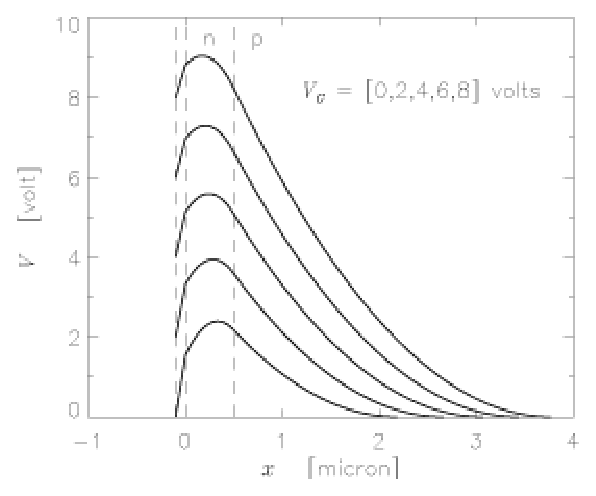
\includegraphics{CCD_burchan.eps}
  \caption{Buried channel potential well.}
  \label{CCD.figburchan}
\end{figure}


\subsection{Depletion}

At the n-p junction mobile carriers from both sides (electrons form
the n-side and holes from the p-side) will tend to diffuse across the
junction and recombine with the opposite type carriers from the other
side. In this way a region on both sides of the junction will be
depleted of carriers, but with space charge densities determined by
the dopant concentrations, $N_D$ and $N_A$, respectively. Left to
itself a contact potential of approximately 0.7 V will be established
across the n-p junction, creating an electric field directed from the
n-side to the p-side and of sufficient strength to stop further
diffusion of carriers across the junction\footnote{There are in fact
  small currents, even in equilbrium, but in that case they are equal
  such that $I_{\rm r}=I_{\rm g}$. The first {\it recombination
    current}, $I_{\rm r}$ is due to the majority carriers that are
  able to overcome the potential barrier $V_{\rm b}$, cross the
  depletion barrier, and undergo recombination. $I_{\rm r}$ has two
  components; one caused by n-side electrons, the other by p-side
  holes. The magnitude of this current will depend on the temperature
  and on the size of the barrier. The second {\it generation current},
  $I_{\rm g}$, is due minority carriers and flows in the opposite
  direction. The minority carriers are thermally ionized
  conduction-band electrons on the p-side and valence band holes on
  the n-side, which defuse away from their creation sites. If they
  reach the depletion region, they will be swept across. Diffusion
  speed outside the depletion region will depend on the temperature
  and the impurity concentration, but $I_{\rm g}$ is independent of $V_{\rm b}$}.

A potential bias applied across the n-p junction will disturb this
equilibrium. For a forward bias, acting to reduce the self-generated
electric fields at the junction, the diffusion of majority carriers
from both sides will continue and an electric current will flow across
the junction. For a reverse bias the self-generated electric field
will be strengthened, driving majority carriers on both sides further
away from the junction and increasing the width of the depletion
region.

An analysis similar to the one above will show that the widths of the
depletion layers, $x_n$ and $x_p$, on the two sides of the junction
are given by
\begin{equation}
  x_n = \frac{N_A}{N_D} \, x_p,
 \label{eq:npjunction1}
\end{equation}
with
\begin{equation}
  x_p = \sqrt{\frac{2\epsilon_{si} N_D}{eN_A(N_A+N_D)} \, V_{\rm ref}}. 
 \label{eq:npjunction2}
\end{equation}
The situation is illustrated in figure \ref{CCD.figjunction}.

\begin{figure}[h]
  \centering
	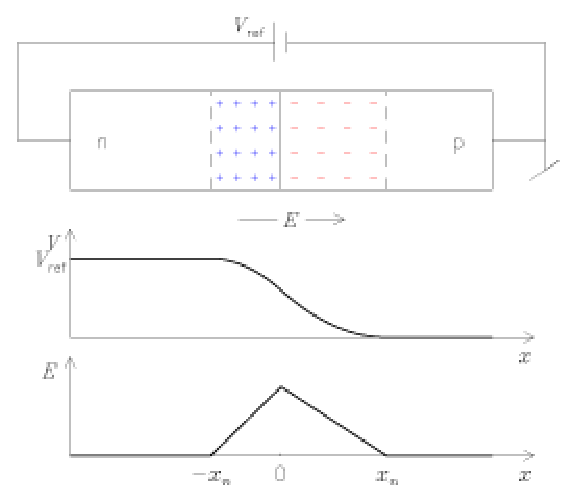
\includegraphics{CCD_junction.eps}
  \caption{n-p junction depletion region.}
  \label{CCD.figjunction}
\end{figure}

Similarly, with the n-channel potential lying above the gate
potential, the electric field near the oxide-silicon interface will
drive n-channel majority carriers away from this interface. This
creates another depletion region starting from the oxide-silicon
interface. With increasing $V_{ref}$ (the potential of the non-depleted
and therefore conducting part of the n-channel) relative to the gate
potential $V_G$, the width of the gate-induced depletion region
increases. Eventually, the two depletion regions from the n-p junction
and the oxide-silicon interface grow together. This occurs when
$V_{max} = V_{ref}$. At this point the voltage generator supplying the
$V_{ref}$ bias to the n-channel will lose control. The n-channel is
no longer conducting and the gate potential $V_G$ will take control
and govern the subsequent process. This is also the necessary
initialization requirement for the buried channel CCD to work as a
photo-detector.

The n-p junction described above is an example of a diode: it will
carry positive current in the direction p to n, but not in the reverse
direction. The size of the current will depend on the potential
$V_{\rm ext}$ applied over the diode.
Absorption of a photon in a diode causes an ionization and
the creation of a conduction band electron and valcence bond
hole. This adds a new contribution to the generation current dependent
on $\phi$, the number of photons that enter the detector per
second. The total current will then be something like
\[
I_{T}=-q\phi\eta+I_{\rm r}+I_{\rm g}
\]
where $\eta$ is a factor that depends on the fraction of incident
photons that are absorbed as well as the probability that a generated
charge carrier will cross the junction before
recombining. Electron-hole pairs created in the depletion zone are
immediately swept apart by the strong electric field there, while
those created outside must first diffuse to the diffusion zone and can
therefore recombine before reaching that far. 

A light sensitive diode can be used in several ways:
\begin{itemize}
\item As a {\it photo-conductor} where a battery holds the external voltage
  to a constant value and the current is a linear function of the
  incident photon flux.
\item As a {\it power-cell} the diode is connected to a constant-load
  resistance, and the power output depends on the incident photon
  flux. This is the principle behind solar power cells.
\item In the {\it photovoltaic} mode current from from the diode
  is held at zero, making it a stroage capicitor, and the voltage
  across it is a non-linear function of the photon flux.
\end{itemize}

\subsection{Storage capacity}

As the CCD detector is subsequently illuminated, the generated
photoelectrons will be collected in a region around the maximum
potential $V_{max}$ in the n-channel. This region therefore becomes
non-depleted, with part of the space charge density of the donor ions
neutralized by the photo-electron space charge density. This in turn
means that the potential maximum starts to decrease and the charge
collection region to widen. 

Indeed, we expect a flat-topped potential distribution within the
photo-electron collection region. Due to the presence of the
photo-electrons, this region will be electrically conducting and where
the internal electric field and the net space charge density
from donor ions and photo-electrons both vanish. The width $\Delta x$
of the flat-topped potential part is therefore determined by the
relation
\begin{equation}
  \Delta x = -\frac{\cl N}{N_D},
\end{equation}
where $\cl N$ is the collected number of photo-electrons per unit
detector area.

The analysis of the buried channel MOS capacitor with photo-electrons
present is rather similar to the one carried out above. The Poisson
equation now reads
\begin{equation}
  \dd{V}{x} = \left\{ \begin{array}{ll} 
	0 & -d < x < 0 \\
	\frac{\displaystyle -eN_D}{\displaystyle \epsilon_{si}} \quad &
	0 < x < t-\Delta x -x_n \\
	0 & t-\Delta x -x_n < x < t -x_n \\
	\frac{\displaystyle -eN_D}{\displaystyle \epsilon_{si}} \quad &
	t-x_n < x < t \\
	\frac{\displaystyle eN_A}{\displaystyle\epsilon_{si}} & 
	t < x < t+x_p \\
	0 & t+x_p < x
  \end{array} \right.
  \label{CCD/.Poissonburph}
\end{equation}
with solution
\begin{equation}
  V(x) = \left\{ \begin{array}{ll} 
	V_G-E_{ox}(x+d) & -d < x < 0 \\
	V_{max} - \frac{\displaystyle
	eN_D}{\displaystyle 2\epsilon_{si}} (x-t+\Delta x +x_n)^2 \quad & 
	0 < x < t-\Delta x - x_n \\ 
	V_{max} & t-\Delta x - n_n < x < t - x_n \\
	V_{max} - \frac{\displaystyle
	eN_D}{\displaystyle 2\epsilon_{si}} (x-t+x_n)^2 \quad & 
	t - x_n < x < t \\ 
	\frac{\displaystyle eN_A}{\displaystyle
	2\epsilon_{si}}(x-t-x_p)^2 & t < x < t+x_p \\
	0 & t+x_p < x.
	\end{array} \right.
\end{equation}
The boundary conditions (\ref{CCD.xn})-(\ref{CCD.VG}) are still
valid. We note that the given form of the solution ensures that the
boundary conditions at the borders of the charge collection region are
automatically satisfied. The solution (\ref{CCD.xp}) is still
valid, but the definitions of $x_1$ and $x_2$ in (\ref{CCD.x12}) have
to be replaced by
\begin{equation}
  x_1^2 = \frac{N_D}{N_A}\left[(t-\Delta
  x)^2+\frac{2\epsilon_{si}}{\epsilon_{ox}}(t-\Delta x)d \right] 
  \quad {\rm and} \quad
  x_2 = t-\Delta x+\frac{\epsilon_{si}}{\epsilon_{ox}}d.
  \label{CCD.x12ph}
\end{equation}

In figure \ref{CCD.figburchanph} the potential structure for a given
gate voltage $V_G$, but for different values $\cl N$ of collected
photo-electrons per unit detector area is given. The parameters for
the MOS capacitor are identical to that of figure~\ref{CCD.figburchan}. 
With $\cl N = 15\times 10^{14}$ m$^{-2}$ the
charged region is less than 40~nm away from the oxide-silicon
interface.

We conclude that there will exist an upper limit to how much charge
can be stored in the device. An over exposure of one pixel element
will mean that surplus photo-electrons will start to leak into
neighboring pixels, producing a ``blooming'' effect in the image.


\begin{figure}[h]
  \centering
	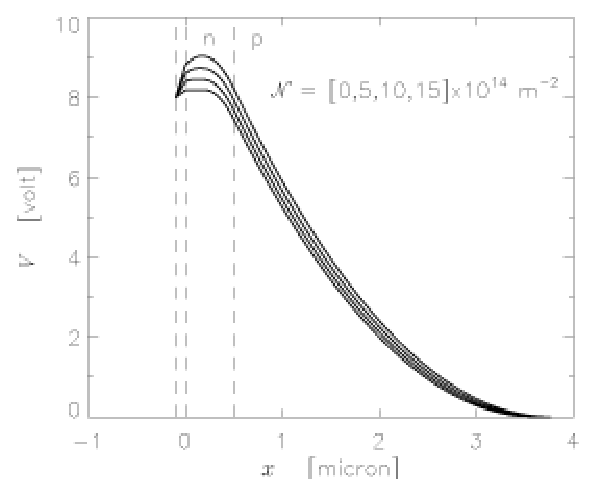
\includegraphics{CCD_burchanph.eps}
  \caption{Buried channel potential structure with photo-electrons present.}
  \label{CCD.figburchanph}
\end{figure}




\section{The charge transfer process} 

After the illuminated charge generation phase the collected charges
need to be transfered to a suitable charge measuring circuitry. In a
three-phase CCD array each pixel is supplied with three separate gate
electrodes as illustrated in figures~\ref{CCD.figpMOS} or
\ref{CCD.fignMOS}, each of these electrodes are connected with the
corresponding electrodes of the neighboring pixels.  In the
collecting phase the middle electrode of each pixel is biased high (10
V), the others low (2 V). Photo-electrons generated over the full pixel
will collect in the potential well existing under the B electrode.
Electrodes A and C act to isolate charges generated in the selected
pixel from similar charges generated in the neighboring pixels.

At the end of the illumination period the charge transfer phase
starts. This is done by applying clocking potentials to the gate
electrodes as indicated in figure~\ref{CCD.figclocking}. The transfer
of electrons from B to C starts by raising the gate electrode C to
high potential. This will widen the potential well under gate B to
also include gate C. The collected electrons will drift to fill the
widened potential well uniformly due to self-induced repulsion. Next
the B-gate potential is lowered, creating fringing fields that push
the remaining electrons under B toward C. In this way the electrons
have been shifted one gate position and are ready to be shifted to
gate A of the next pixel and so on. After three gate shifts the
collected electrons have been moved one pixel.

Optimum performance of the transfer process is achieved for slow slew
rates of the clocking signals. The characteristic RC rise and fall times
 $\tau_{RC}$ of the clocks are therefore often related to the one pixel
transfer time $t_T$ by
\begin{equation}
  \tau_{RC} = \frac{t_T}{12}.
\end{equation}
This is the choice made in figure~\ref{CCD.figclocking}. A typical
value of the transfer time may be $t_T = 1$ $\mu$s.

\begin{figure}[h]
  \centering
	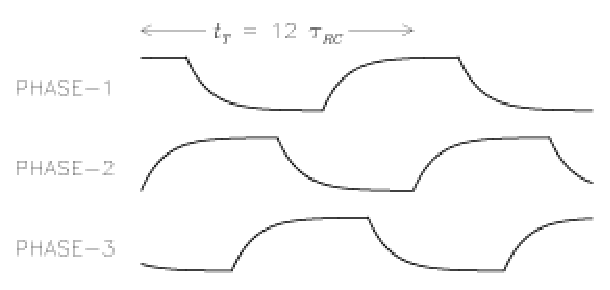
\includegraphics{CCD_clocking.eps}
  \caption{Clocking signal for three-phase CCD}
  \label{CCD.figclocking}
\end{figure}


\section{Charge measurements} 

The final operational phase of the CCD detector is the measurement of
the charges accumulated in the different pixels during the exposure
time. This is accomplished by dumping the transfered charges on to a
small capacitor connected to a MOSFET amplifier. The MOSFET amplifier
is the only active element of the CCD detector, that is, it is the
only element that requires power. The individual pixel elements made
up of MOS capacitors are themselves passive elements.

The output amplifier generates a voltage proportional to the charge
transfered, the larger voltages the smaller the capacitance of the
output capacitor. Important engineering design criteria for the output
stage is to minimize the noise generation in the MOSFET
amplifier. This can be achieved by cooling the CCD detector to
temperatures down to about - 90$^\circ$C.  Modern
high-performance CCDs have achieved remarkable noise level
equivalents down to less than 2 (elementary) electron charges.

\section{Dark currents}

Operating the CCD detector under reduced temperatures will also reduce
problems related to dark currents in the MOS capacitors. The basic
underlying assumption of the CCD as a photon counting device is that
the photoelectrons are the only source of the accumulated charge. This
assumption is challenged by the existence of dark currents. Dark
currents occur naturally in semiconductors through thermal generation
of charge carriers. Dark current generation occurs independent of the
illumination state of the semiconductor, thus its name. The only way
of reducing this error source for a given detector is to lower the
operating temperature. The dark current level for a given temperature
is, however, strongly dependent on the fabrication process and the
quality of the silicon used in the production.

There are three main regions that contribute to dark currents: the
neutral bulk material below the potential well, the depleted material
within the potential well and the oxide-silicon interface. Normally
the latter is the more important one. Dark current carriers are
generated through the presence of midband energy states halfway
between the valence and conduction bands. These states are associated
with imperfections or impurities within the semiconductor or at the
oxide-semiconductor interface. They promote dark currents by acting as
stepping stones for two-step thermal transitions of electrons and
holes between the valence and conduction bands. Any electron raised to
the conduction band through this process in the depleted region will
be collected in the potential well together with the desired
photoelectrons. Corresponding electrons generated in the field-free
region outside the depletion region may enter this region through a
diffusion process, then to be collected by the existing electric field.
 
The temperature variation of the dark current in the CCD is well
described by the formula
\begin{equation}
  I_d = C \cl T^{3/2} \exp(-U_g/\cl T),
\end{equation}
where $C$ is a constant for each detector and $U_g$ is the silicon
band-gap energy. The band-gap energy is found to follow the empirical
formula (in eV units)
\begin{equation}
  U_g = 1.1557 - \frac{7.021\times 10^{-4}\, T^2}{1108+T}
\end{equation} 
with temperature $T$ given in degrees K. In figure \ref{CCD.figdark}
the dark current for the CCD normalized to unity for room temperature
($T = 300$ K) is plotted.  One should bear in mind that the operating
temperature of the CCD cannot be made arbitrarily low. To function the
temperature of the CCD must be high enough that the dopant atoms
remain in ionized state in the lattice and thus contribute to the
formation of potential wells. This requires operating temperatures
exceeding 70 K.

\begin{figure}[h]
  \centering
	\includegraphics{CCD_dark.eps}
  \caption{Normalized dark current as a function of temperature }
  \label{CCD.figdark}
\end{figure}

\section{CCD summary, problems and corrections}

For typical noise levels and pixel capacities, astronomical CCDs have dynamic
ranges of $100\,000$ to $500\,000$.

A major problem is the noise produced by cosmic rays. A single cosmic ray
particle coming through one of the pixels of the detector can cause a large
number of ionizations. The resulting electrons accumulate in the storage 
region along with those produced by photons. These are usually recognizable
by the observer as `spikes' in the image. Replacing such spikes is possible
by using the average of the surrounding pixels, but this does not retrieve 
the original information lost. In addition the correction must often be done
`by hand' which can be time consuming. Automatic removal of spikes is 
sometimes possible given several individual images of the same object or a 
good model of the data --- but such automatic removal is difficult and 
can become a `black art'. 

Another defect of CCDs is the variation in the background noise between 
pixels. There may be large-scale variations of 10--20~\% over the whole
sensitive area, and there may be individual pixels with permanent high levels.
The first problem can be reduced by flat fielding if its effect can be 
determined by observing a uniform source. The effect of a single hot spot
may also be reduced in signal processing by replacing it with an average of
its neighbors. However, the hot spot pixel is often also a poor transporter 
of charge resulting in a spurious line being introduced into the image.

Yet another problem is that of cross talk or blooming. This occurs when 
electrons stray to nearby pixels. This especially effects rear illuminated 
CCDs as in them electrons are produced quite far from the electrodes. This
is the reason rear illuminated CCDs are thinned; {\it ie} to reduce this 
distance. It will also occur for any CCD where the accumulating charge nears
its maximum capacity. 

\section{Other types of detectors}

In these notes we have concentrated almost exclusively on CCD's, but one should
be aware that also other types of detectors exist. These are covered were
summarily here and in somewhat more detail in chapter~1 of Kitchin's 
{\it Astrophysical Techniques}.

\subsection{Photomultiplyers}

Electron photomultiplyer phototubes were once the workhorse of optical 
astronomy. They continue to be used when individual photons need to be
detected  as in neutrino and cosmic ray \^Cerenkov detectors or when very
rapid responses are required as in observations of occultations.

Photomultiplyers detect photons through the photoelectric effect. A 
photoemitter is coated on to the cathode and this is at a negative potential
of some 1000~V. Once a photoelectron has escaped from the photoemitter, it
is accelerated by an electric potential until it strikes a second 
electron emitter. The primary electron's energy then goes into pair production
and secondary electrons are emitted from the substance in a manner analogous
to photo-electron emission. Several secondary electron emissions result 
from a single primary electron. The secondary emitter is coated onto dynodes
that are successively more positive than the cathode by 100~V or so for each
stage. The various electrodes are shaped and positioned so that the electrons
are channelled towards the correct next electrode in the sequence after 
each interaction. The final signal pulse may contain $10^6$ electrons for each
incoming photon. 

\subsection{Superconducting tunnel junction detectors (STJs)}

Kitchin mentions that a possible replacement of CCDs could come in the form
of superconducting tullel junction detectors (STJ). At temperatures
below $T_{\rm c}$, an unlimited number fo superconducting states exist
at an energy $\Delta$ below the Fermi level. Single electrons will
therefore occupy only states of energy $(E_{\rm F}-\Delta$ or
  lower. $\Delta$ is a strong function of temperature rising from zero
  at $T_{\rm c}$ to a maximum $\Delta_{\rm m}$ at temperatures below
  about $0.3T_{\rm c}$. The value of $\Delta_{\rm m}$ measures the
  binding energy per electron of a {\it Cooper pair} is very small;
  for example $1.4\times 10^{-4}$~eV for Pb, which is typical. If a
  superconductor is to absorb a photon it must have energy larger than
  $2\Delta$ so that a Cooper pair can be broken up and both electrons
  promoted to excited states in the ``conduction'' band. These
  electrons will have quantum characteristics that differ from
  energetic electrons in an ordinary metal, and are therefore termed
  {\it quasiparticles}. The number of states available to
  quasiparticles at energies just above the gap is very large.

The STJ can operate 
from the UV to the longwave infrared, and also in the X-ray region.
Its operating principle is based on a {\it Josephsons junction}. This has two 
superconducting layers separated by a insulating layer that is thin
enough (of order 1~nm) to permit quantum mechanical tunneling. A
junction can be arranged as a light-detecting diode by applying a
positive bias voltage less than $V^{+}=2\Delta/q$ to one of the
superconductors and a magnetic field applied parallell to the
junction. If the junction is very cold all excited states are
empty. In a normal Josephson junction Cooper pairs could tunnel across
the insulating layer to the superconductor with applied voltage
$V^{+}$, but the applied magnetic field hindres this, and the diode
does not conduct.

If the superconductor without applied voltage absorbs a photon of
energy $hc/\lambda$ it receives enough energy to break apart mulitple
Cooper pairs, promoting a maximum of $hc/\lambda\Delta$ electrons into
excited states. These quasiparticles {\it can} tunnel across the
insulator, and those that do produce a current pulse that is inversely
proportional to the wavelength $\lambda$ of the exciting photon.

The STJ detector can therefore count individual incoming photons and
determine their wavelength, from X-ray to infrared, of each. This is a
technology still in development, but some practical multi-pixel
STJ-based detectors have begun to appear at telescopes.

\subsection{Other types}

\noindent{\it Photvoltaic cells.} These are also known as photodiodes,
photoconductors, and barrier junction detectors. The idea is to use the
properties of a p-n junction in a semiconductor. When such a junction
is in equilibrium electrons and holes have diffused across the
junction until a sufficient potential difference is set up to halt the
flow. The two Fermi levels are then coincident and the potential
across the junction is equal to their original difference. If now
light falls on the junction it can generate electron-hole pairs in
both the n-type and the p-type materials. The electrons in the
conduction band of the p-region will be attracted towards the n region
by the intrinsic potential difference across the junction, and they
will be free to flow in that direction. The holes in the valence band
of the p-type material will be opposed by the potential and will not
move. In the n-type region the electrons will be similarly trapped
while the holes will be pushed across the junction. Thus a current is
generated by the illuminating radiation and this may simply be
monitored and used as a measure of light intensity. For use as a
radiation detector the p-n junction often has a region of undoped (or
intrinsic) material between the p and n regions in order to increase
the size of the detecting area. These devices are known as p-i-n
junctions, and their operating principle does not differ fro that of
the simple p-n junction.

\noindent{\it Thermocouples.} Two dissimilar metals in contact can
develop a potential difference across their junction. This is called
the Seebeck effect. The position of the Fermi level will change with
temperature and the change in Fermi level may not be the same in two
dissimilar metals, and so at the junction the difference between the
two Fermi levels will vary with temperature. In a thermocouple, two
dissimilar metals are joined into a circuit that incorporates a
galvanometer. When one junction is at a different temperature from the
other, their Seebeck potentials differ and a current flows through the
circuit. 

A practical thermocouple for radiation detection is made from two
metals in the form of wires that are twisted together and blackened to
improve their absorption. The other junction is kept in contact with
something with a large thermal inertia so that it is kept at a
constant temperature. Several thermocouples are usually connected
serially so that their potentials combine. This is called a {\it
  thermopile}.

Practical thermocouples and thermopiles are usually made from antimony
and bismuth or from nickel and various mixtures of copper, silicon,
chromium, aluminium etc. They are useful wide-band detectors,
especially for infrared work. Their simplicity of operation and
robustness has led to many application for them despite their
relatively low sensitivity.

\noindent{\it Phototransistors.} These are of little direct use in
astronomy because of their low sensitivity. They consist simply of a
p-n-p or n-p-n transistor with the minority current carriers produced
by the illumination instead of the normal emitter. Thus the current
rises with increasing radiation and provides a measure of its intensity.

\noindent{\it Charge injection devices} (CID) -- detection method identical to CCD, 
the difference lies in the read out system. 

\subsection{Infrared detectors}

Many of the detectors mentioned above have some infrared (IR) sensitivity, 
especially out to 1~$\mu$m. At longer wavelengths, other types of detectors
are needed. The IR region is conventionally divided into three: the near
(NIR), 0.7--5~$\mu$m, the mid (MIR), 5--30~$\mu$m and the far (FIR), 
30--1000~$\mu$m. All IR detectors need to be cooled, with the longer the
operating wavelength, the colder the required temperature. Thus in the 
NIR liquid nitrogen (77~K) suffices, in the MIR liquid helium (4~K) is 
needed, while one must operate at temperatures down to some 100~mK in the 
FIR. Currently there are two types of detector in the IR: the photoconductor
of the NIR and MIR (and somewhat into the FIR) and the bolometer for the
FIR.

\noindent{\it Photoconductive cells} exhibit a change in conductivity with the 
intensity of their illumination. The mechanism for that change is the 
absorption of radiation by the electrons in the valence band of a 
semi-conductor and their consequent elevation to the conduction band. The
conductivity therefor increases with increasing illumination, and is monitored
by a small bias current. These cells have been assembled into arrays of 
up to $2048\times 2048$ for the NIR and $1024\times 1024$ for the MIR, 
though at the long wavelength end of the MIR arrays of some hundred cells is
the maximum. In the FIR sizes are still only up to $32\times 32$. Unlike
CCDs infrared arrays are read out pixel by pixel. 

\noindent{\it Bolometers} are devices that change their electrical
resistivity in response to heating by illuminating radiation. At the
simplest, two strips of material are used as the arms of a Wheatstone
bridge. When one is heated by the radiation its resitance changes and
so the balance of the bridge alters. 

\section{Noise}

In the absence of noise any detector would be capable of detecting any source,
however faint. A minimum signal to noise ratio of unity is required for 
detection. However, most research work requires signal to noise ratios of
at least 10, and preferably 100 or 1000. 

Noise sources can be separated into four classes: {\it intrinsic noise} 
originating from the detector, {\it signal noise} arising from the character
of the of the incoming signal, {\it external noise} e.g. spurious signals
from cosmic rays and the like, {\it processing noise} from amplifiers and
similar used to convert the signal from the detector into a usable form.

{\it Intrinsic noise} in solid state devices comes from four sources.
\begin{enumerate}
\item Thermal noise arises in any resistive material. It is due to the thermal
motion of the charge carriers. 
\item Shot noise occurs in junction devices and is due to variation in 
the diffusion rates in the neutral zone of the junction because of random
thermal motions. 
\item Generation-recombination noise is caused by the fluctuation in the
rate of generation and recombination of thermal charge carriers. 
\item Flicker noise, or ($1/f$ noise), occurs when the signal is modulated
in time, either because of intrinsic variations or because it is being
`chopped' (i.e. source and background are alternately observed). 
\end{enumerate}

{\it Signal noise} can be present for a variety of reasons. One example is
background noise. Noise also comes from the quantum nature of light. At
low signal levels photons arrive at the detector sporadically. A Poisson
distribution gives the probability of arrival, and this has the standard
deviation of $\sqrt{n}$ where $n$ is the mean number of photons per unit
time. 


\section{Exercises}

\begin{enumerate}
\item Describe, in detail, how two phase and virtual phase CCDs move charges
compared to three phase CCDs.
\item Re-derive the expressions for the total voltage drop and for thickness 
of the depletion region $x_d$ for a surface channel potential well. Reproduce
with {\tt idl} the plot of the potential versus depth for gate voltages of 
4, 8 and 12~V for a depleted CCD using the numbers given in the lecture notes.
\item How many electrons $\cal{N}$ per unit interface area and over time $\tau$
can be collected before the thickness of the depletion region $x_d$ 
approaches zero? How would you convert the number of electrons into a limiting
photon flux?
\item Re-derive the expressions for the potential in an illuminated buried
channel CCD, making sure that all the boundary conditions are satisfied (and 
understood!). How would you derive a limit for the storage capacity given 
in number of photoelectrons $\cal{N}$ of the CCD using this
expression?
\item Derive equations~\ref{eq:npjunction1} and \ref{eq:npjunction2}
  giving the size of the depletion region in a n-p diode with reverse
  bias $V_{\rm ref}$.
\item What is a photomultiplyer? (We will discuss photomultiplyers
  further when we cover {\it photometry}.)
\item Give a basic description of a {\it Superconducting tunnel
    junction detector (STJ)}. Find examples of current
  astronomical use (if any) and future prospects.
\item Give a basic description of how {\it photovoltaic cells}, 
{\it photoconductive cells}, and {\it bolometers} work and for which regions
of the spectrum they are used for. Find expamples of modern telescopes/instruments
(space or ground based) on which such measurement techniques are used.
\end{enumerate}

%\end{document}


% Lecture notes on Chapter 4:
\documentclass{article}
\usepackage{wasysym}
\usepackage{graphics}
\usepackage{psfig}
\newcommand{\bc}{\begin{center}}
\newcommand{\ec}{\end{center}}
\newcommand{\be}{\begin{equation}}
\newcommand{\ee}{\end{equation}}
\newcommand{\bea}[1]{\begin{eqnarray}\label{#1}}
\newcommand{\eea}{\end{eqnarray}}
\newcommand{\bua}{\begin{eqnarray*}}
\newcommand{\eua}{\end{eqnarray*}}
\newcommand{\infint}{\int_{-\infty}^{\infty}}
\newcommand{\dd}[2]{{{d#1}\over{d#2}}}
\newcommand{\ddt}[1]{\dd{#1}{t}}
\newcommand{\dddt}[1]{\dd{^2#1}{t^2}}
\newcommand{\aver}[1]{\langle{#1}\rangle}
\def\labs{\mid\!}
\def\rabs{\!\mid}
\begin{document}
\section*{Lecture notes 4: Fourier Analysis}

\subsection*{Definitions}

There are many common (and confusing, but ultimately trivial!)
differences in defining the {\it Fourier transform}. One common 
definition is 
\[
F(\nu)=\infint f(t)e^{-i2\pi\nu t}dt
\]
Thus $F(\nu)$ gives the wavenumber representation of the function
$f(t)$. The inverse transform can be written 
\[
f(t)=\infint F(\nu)e^{i2\pi\nu t}d\nu
\]
$F(\nu)$ is in general a complex function whose interpretation may be
aided by expression in the polar coordinate form
$F(\nu)=A(\nu)e^{i\phi(\nu)}$, where $A(\nu)$ and $\phi(\nu)$ are real
functions where $A(\nu)=\labs{F(\nu)}\rabs$ is the amplitude and $\phi(\nu)={\rm
  arg}[F(\nu)]$  is the phase. Note that we then can write the inverse 
transform as 
\[
f(t)=\infint A(\nu)e^{i[2\pi\nu t+\phi(\nu)]}d\nu,
\]
which is seen to be a recombination of all the frequency components of
$f(t)$. Each component is a complex sinusoid of the form $e^{2\pi i\nu t}$
whose amplitude is $A(\nu)$ and whose initial phase (at $t=0$) is
$\phi(\nu)$. This interpretation of the Fourier transform clearly
shows its relation to the {\it Fourier series}\footnote{Note that by 
using Euler's formula $e^{inx}=\cos(nx)+i\sin(nx)$ a more concise (and
modern) form can be used: $f(x)=\sum_{n=-\infty}^\infty c_n e^{inx}$
with $c_n={1\over 2\pi}\int_{-\pi}^{\pi} f(x)e^{-inx}dx$.} 
\[
f(x)={a_0\over 2}+\sum_{n=1}^\infty[a_n\cos(nx)+b_n\sin(nx)]
\]
with coefficients given by 
\bua
a_n & = & {1\over\pi}\int_{-\pi}^\pi f(x)\cos(nx)dx \\
b_n & = & {1\over\pi}\int_{-\pi}^\pi f(x)\sin(nx)dx.
\eua

It is common to perform the substitution $\nu={\omega/2\pi}$ which
gives
\bua
F(\omega)&=&\infint f(t)e^{i\omega t}dt \\
f(t)&=&{1\over 2\pi}\infint F(\omega)e^{-i\omega t}d\omega
\eua

\subsection*{Properties}

Fourier transforms exhibit a number of properties that are very
useful:
\begin{itemize}
\item Linearity \[ af(t)+bg(t)\Longleftrightarrow
  aF(\omega)+bG(\omega) \]
\item Multiplication \[ f(t)g(t)\Longleftrightarrow{1\over
    2\pi}(F\otimes G)(\omega) \]
where we define the {\it convolution} $\otimes$ as \[
K(\omega)\equiv\infint F(\omega')G(\omega-\omega')d\omega' \]
\item Convolution \[ (f\otimes g)(t)\Longleftrightarrow
  F(\omega)G(\omega) \]
\item Conjugation \[ \overline{f(t)}\Longleftrightarrow\overline{F(-\omega)} \]
\item Scaling \[ f(at) \Longleftrightarrow {1\over
    \labs a\rabs}F\left({\omega\over a}\right) \]
 \item Time reversal \[ f(-t) \Longleftrightarrow F(-\omega) \]
\item Time shift \[ f(t-t_0) \Longleftrightarrow e^{-i\omega
    t_0}F(\omega) \]
\item Parsevals theorem \[ \infint f(t)\overline{g(t)}dt = {1\over
    2\pi}\infint F(\omega)\overline{G(\omega)}d\omega \]
\end{itemize}

The {\it correlation} of two functions, denoted by ${\rm Corr}(g,h)$, is defined
\[
{\rm Corr}(g,h)\equiv\int_{-\infty}^\infty g(t'+t)h(t')dt'
\]
The correlation is a function of $t$, called the {\it lag}. The ``Correlation theorem'' states that 
\[ {\rm Corr}(g,h) \Longleftrightarrow  G(f)\overline{H(f)} \]
if $g$ and $h$ are real functions, as we expect for our applications [otherwise the expression on 
the right hand side of the correlation theorem is $G(f)H(-f)$.] The correlation of a function with itself is called the {\it autocorrelation}. In this case we have 
\[ {\rm Corr}(g,g) \Longleftrightarrow  \labs G(f)\rabs^2 \]
which is also known as the ``Wiener-Khinchin theorem''. The {\it total power} in a signal
can be computed from the autocorrelation of that signal and following Parseval's theorem
we can write
\[ {\rm Total~Power}\equiv\int_{-\infty}^{\infty}\labs g(t)\rabs^2dt
  =\int_{-\infty}^{\infty}\labs G(f)\rabs^2df.
\]
Often one desires to know how much power is contained in the frequency interval between $f$ and $f+df$. In this case it is often not
interesting to distinguish  between positive and negative $f$, but rather regard $f$ as varying from $0$ (zero frequency or DC) to $+\infty$. In this case we define the {\it one-sided power spectral density} of the function $g$:
\[ P_g(f) \equiv \labs G(f)\rabs^2+\labs G(-f)\rabs^2\qquad 0\le f<\infty,\]
when $g$ is real the two terms in the equation above are equal, so 
\[ P_g(f)=2\rabs G(f)\labs^2.\]
\subsection*{Sampling Theorem and Aliasing}

We will in general be dealing with functions $h(t)$ which are sampled
at evenly spaced intervals in time (or space). Let $\Delta$ denote the 
time (space) interval between consecutive samples.

For any sampling interval $\Delta$, there is a special frequency
$\nu_c$ called the {\it Nyquist frequency} given by 
\[
\nu_c\equiv{1\over 2\Delta}
\]
The critical sampling of a sine wave is two sample points per
cycle. There are two aspects of the critical frequency. First, if the
original signal is bandwidth limited to frequencies smaller than
$\nu_c$ then the function is completely determined by its discrete
samples. This is the {\it sampling theorem}. However, if a signal is
{\it not} bandwidth limited to less than the Nyquist frequency then
the power that lies outside the range $-\nu_c<\nu<\nu_c$ is spuriously
moved into that range. This phenomena is called {\it aliasing}. 

\subsection*{FFTs}

Let us now estimate a Fourier transform from a finite number of sampled points.
Suppose that we have $N$ consecutive sampled values
\[
h_k\equiv h(t_k) \qquad t_k\equiv k\Delta \qquad k=0,1,2,\ldots,N-1 
\]
so that the sampling interval is $\Delta$. Also assume $N$ is even. With $N$ 
numbers of input, we cannot produce more than $N$ independent numbers of 
output. So, instead of trying to estimate the Fourier transform $H(\nu)$ at 
all values of $\nu$ in the range $-\nu_c$ to $\nu_c$, let us seek estimates 
at only the discrete values
\[
\nu_n\equiv{n\over N\Delta},\qquad n={-N\over 2},\ldots,{N\over 2} 
\]
The extreme values of $n$ correspond to the lower and upper values of the 
Nyquist critical frequency range. 

The remaining step is to approximate the continuous transform by a discrete 
sum
\[
H(\nu_n)=\infint h(t)e^{2\pi i \nu_nt}dt\approx \sum_{k=0}^{N-1}h_ke^{2\pi i\nu_nt_k}\Delta=\Delta\sum_{k=0}^{N-1}h_k e^{2\pi ikn/N}
\]
The final summation is called the {\it discrete Fourier transform} of the $N$ 
points $h_k$. Let us denote it by $H_n$:
\be
H_n\equiv\sum_{k=0}^{N-1}h_k e^{2\pi ikn/N}
\label{eq:discrete-fourier}
\ee
Up to now we have taken the view that index $n$ varies from $-N/2$ to $N/2$. 
However, since it is clear that equation~\ref{eq:discrete-fourier} is 
periodic in $n$ we also have that $H_{-n}=H_{N-1}$. With this in mind it is 
customary to let $n$ vary from $0$ to $N-1$ (one period). When this convention
is followed the {\it zero} frequency corresponds to $n=0$, positive 
frequencies $0<\nu<\nu_c$ correspond to values $1\le n\le {N/2}-1$, while
negative frequencies $-\nu_c<\nu<0$ correspond to ${N/2}_1\le n \le N-1$. The
value $n={N/2}$ corresponds to both $\nu=\nu_c$ and $\nu=-\nu_c$.

The discrete {\it inverse} transform which recovers $h_k$ form the $H_n$ is
\[
h_k={1\over N}\sum_{n=0}^{N-1}H_n e^{-2\pi ikn/N}
\]

How do we implement the discrete transform in code? The brute strength 
approach takes of order $N^2$ operations: Define $W$ as the complex number
\[
W\equiv e^{2\pi i/N}
\]
Then equation~\ref{eq:discrete-fourier} can be written 
\[
H_n=\sum_{k=0}^{N-1}W^{nk}h_k,
\]
{\it i.e.} the vector $h_k$ is multiplied by a matrix whose $(n,k)^{th}$
element is the constant $W$ to the power $n\times k$. The matrix multiplication
produces a vector result whose components are $H_n$. This multiplication
evidently needs $N^2$ complex multiplications. 

In fact, the discrete Fourier transform can be achieved in $N\log_2 N$ 
operations with an algorithm called the {it Fast Fourier Transform} or 
{\it FFT}. Here is one derivation of the FFT, that of Danielson and Lanczos
in 1942. They showed that a discrete transform of length $N$ can be rewritten
as the sum of two discrete transforms, each of length $N/2$. One of the 
two is formed from the even numbered points of the original $N$, the other 
from the odd-numbered points.
\bua
F_k & = & \sum_{j=0}^{N-1}e^{2\pi ijk/N}f_j \\
    & = & \sum_{j=0}^{{N/2}-1}e^{2\pi i2jk/N}f_{2j}
         +\sum_{j=0}^{{N/2}-1}e^{2\pi i(2j+1)k/N}f_{2j+1} \\
    & = & \sum_{j=0}^{{N/2}-1}e^{2\pi ijk/({N/2})}f_{2j}
         +W^k\sum_{j=0}^{{N/2}-1}e^{2\pi ijk/({N/2})}f_{2j+1} \\
    & = & F_k^e+W^kF_k^o
\eua
$F_k^e$ denotes the $k^{th}$ component of the Fourier transform of length 
$({N/2})$ formed from the even components of the original $f_j$, while $F_k^o$
is the corresponding transform of length $({N/2})$ from the odd components.

This procedure can be applied recursively; having reduced the problem of
computing $F_k$ to that of computing $F_k^e$ and $F_k^o$, one can do the 
same reduction of $F_k^e$ to the problem of computing the transform of 
{\it its} $N/4$ even-numbered inputs data, $F_k^{ee}$, and $N/4$ odd-numbered 
data $F_k^{eo}$. When we start with an original $N$ which is a integer 
power of 2 (one should only use FFTs with $N$ a power of 2, padding the input
data with zeroes is necessary) we can continue applying the Danielson-Lanczos 
method until the original data is subdivided all the way down to transforms
of length one. The Fourier transform of length one is just the identity 
operation that copies its one input number into its output slot. Thus, 
for every pattern of $e$'s and $o$'s numbering $\log_2 N$ in all there is a 
one-point transform that is given by 
\[
F_k^{eoeeoeo\cdots oee}=f_n\qquad {\rm for~some~}n
\]
Which value of $n$ corresponds to which pattern? Reverse the pattern of 
$e$'s and $o$'s, let $e=0$ and $o=1$ and one will have, {\it in binary}, the
value of $n$. This is because the successive subdivisions of the data into 
odd and even are tests of successive least significant bits of $n$. Thus
by rearranging the input vector $f_j$ in bit reversed order so that the 
individual numbers are in the order obtained by bit reversing $j$. The points
are given as one-point transforms. These are recombined with the adjacent 
number to give two-point transforms, then combine adjacent pairs again to 
give 4-point transforms, and so on, using the Danielson-Lanczos formula
at every step.

The FFT therefore has a structure where first the data are sorted into
bit reversed order and thereafter the transforms of length $2,4,8,\ldots,N$
are computed implementing the Danielson-Lanczos formula.

\subsection*{Exercises}

Experiment with the {\tt fft} function in {\tt idl}. First make an $x$-axis, 
{\it eg} {\tt idl> x=findgen(2000)/100.*2.*!pi}
\begin{enumerate}
\item Compute the amplitude of the transform of $f=\sin x$. In plotting this 
amplitude, what should be used for the $x$-axis?
\item What happens if you set the edges of $f$ to zero: {\it eg} multiply $f$
by a step-function $s$ such as {\tt idl> s=fltarr(2000) \& s[200:1800]=1.0}? 
Overplot the amplitude of the transform as you narrow the region of $s$ that is
equal to one.
\item Compute the transform of step-functions of various widths.
\item Add sinusoidal functions to $f$ with different frequencies and check the
resulting transforms. What happens to the transform if you add a constant to 
$f$? 
\item Consider a function $g$ given by the sum of three sinusoidals of differing
frequency. Construct such a $g$ and remove one of the frequencies from $g$ using 
forward and back transforms FFT's in {\tt idl}.
\end{enumerate}

\end{document}

% Lecture notes on Chapter 5:
%\documentclass{article}
%\usepackage{wasysym}
%\usepackage{graphicx}
%\usepackage{bm}
%\usepackage{psfig}
%\newcommand{\bc}{\begin{center}}
%\newcommand{\ec}{\end{center}}
%\newcommand{\be}{\begin{equation}}
%\newcommand{\ee}{\end{equation}}
%\newcommand{\bea}[1]{\begin{eqnarray}\label{#1}}
%\newcommand{\eea}{\end{eqnarray}}
%\newcommand{\bua}{\begin{eqnarray*}}
%\newcommand{\eua}{\end{eqnarray*}}
%\newcommand{\infint}{\int_{-\infty}^{\infty}}
%\newcommand{\dd}[2]{{{d#1}\over{d#2}}}
%\newcommand{\ddt}[1]{\dd{#1}{t}}
%\newcommand{\dddt}[1]{\dd{^2#1}{t^2}}
%\newcommand{\aver}[1]{\langle{#1}\rangle}
%\def\cl#1{{\cal #1}}               % for caligrafic letters
%\def\labs{\mid\!}
%\def\rabs{\!\mid}
%\begin{document}
\section{Lecture notes 5: Diffraction}

Let us now consider how light reacts to being confined to a given aperture. The resolution 
of an aperture is restricted due to the wave nature of light: as light passes through any 
opening it is {\it diffracted} and the wave fronts spread out in a shape given by the 
envelope of Huygens's secondary wavelets which radiate spherically outwards from all points on 
a wave front. These waves travel along every path, from the source to the point of observation,
where they are added together only giving a significant net contribution when they add 
coherently in phase. 

\noindent (In the following I will follow Kip Thorne's lecture notes found at 
\newline{\tt www.pma.caltech.edu/Courses/ph136/yr2004}.)

\subsection*{Helmholtz-Kirchhoff Integral}

Let us restrict attention to the simplest (and, luckily the most
useful) case: a monochromatic scalar wave 
\[
\psi=\psi({\mathbf x})e^{-i\omega t}
\]
with field variable $\psi$ of frequency $\omega=ck$ which satisfies Helmholtz's equation
\be
\nabla^2\psi+k^2\psi=0
\label{eq:helmholtz}
\ee
except at the boundaries. $\psi$ is generally a real physical value, but for convenience we will
use a complex representation. The wave is monochromatic and non-dispersive and the medium is
isotropic and homogeneous so that $k$ can be treated as a constant\footnote{Each of these 
assumptions can be lifted at the cost of introducing technical complications.}. This formalism
is valid for weak sound waves in a fluid and is fairly accurate for the propagation of 
electromagnetic waves in vacuum or in a medium with a constant dielectric constant $\epsilon$. 
In the latter case $\psi$ can be considered as one of the Cartesian components of the electric
or magnetic field vector, e.g. $E_x$ or $B_y$. In vacuum Maxwell's equations imply that 
$\psi=E_x$ satisfies equation~\ref{eq:helmholtz}. 

\begin{figure}[th!]
%  \hfil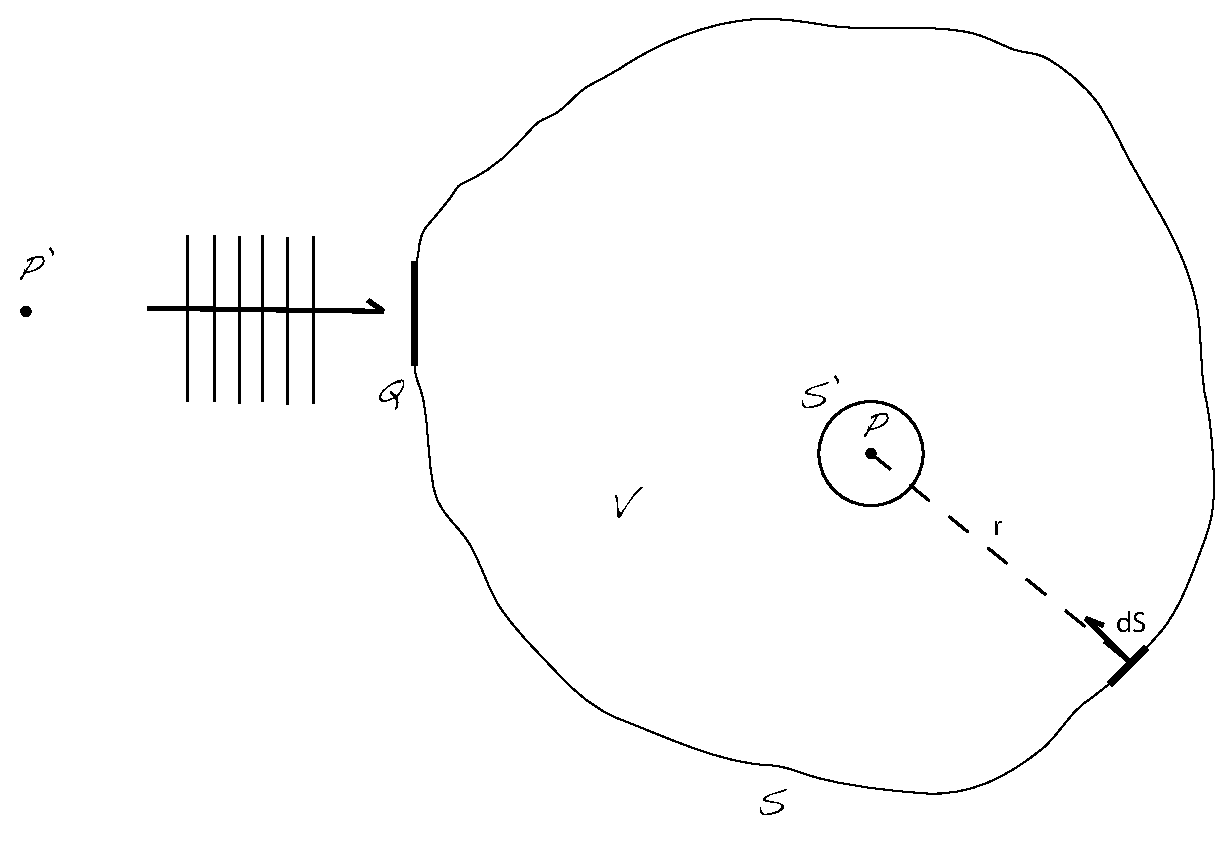
\psfig{file=helmholz-kirchhoff-surface.eps,width=0.7\textwidth}\hfil
	\centering
	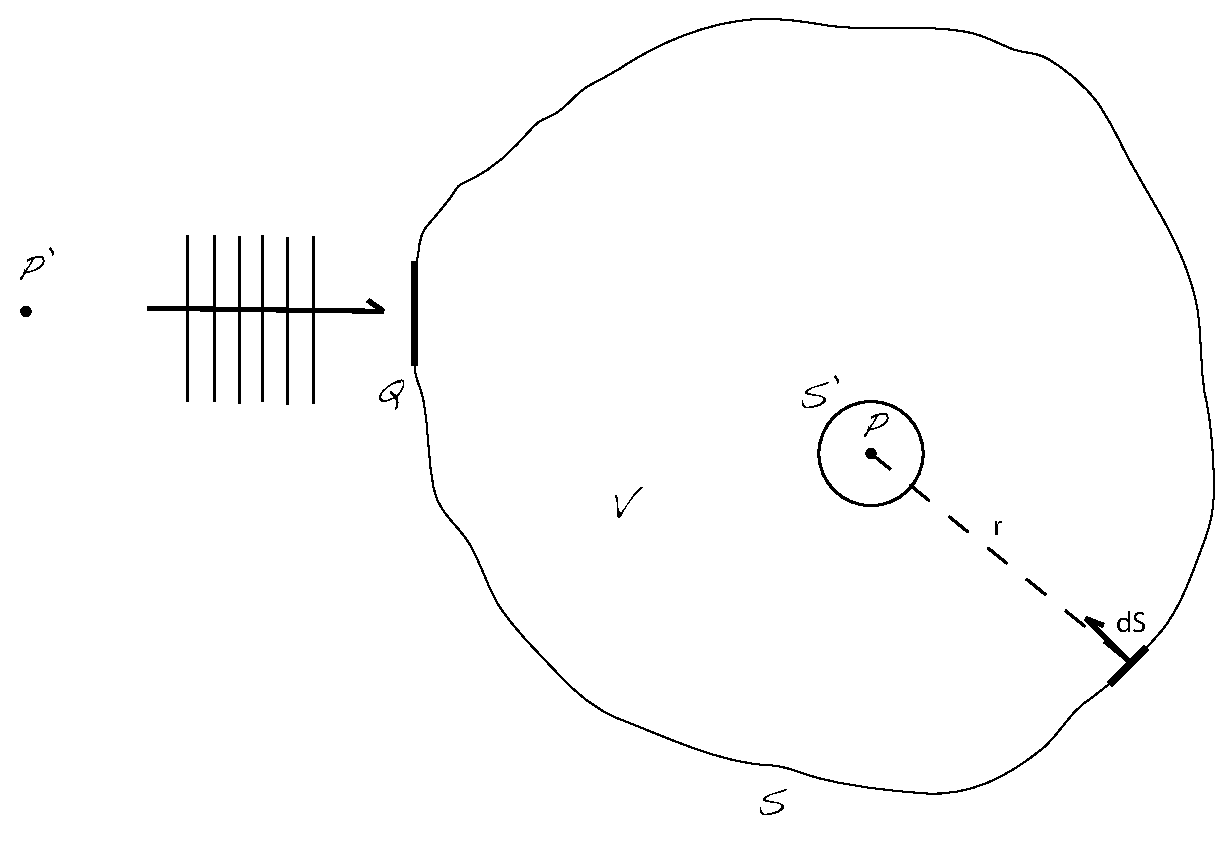
\includegraphics[width=0.7\textwidth]{helmholz-kirchhoff-surface.eps}
  \caption{Surface $\cal{S}$ for the Helmholtz-Kirchhoff integral. The surface
$\cal{S'}$ surrounds the observation point $\cal{P}$ and $\cal{V}$ is the 
volume bounded by $\cal{S}$ and $\cal{S'}$. The aperture $\cal{Q}$, the 
incoming wave to the left of it and the point $\cal{P'}$ are used later in the
text.}
  \label{fig:helmholz-kirchhoff-surface}
\end{figure}

The Helmholtz equation~\ref{eq:helmholtz} is an elliptic, linear, partial differential equation,
and thus permits us to express the value of $\psi_\cl{P}$ of $\psi$ at any point $\cl{P}$ inside
some closed surface $\cl{S}$ as an integral over $\cl{S}$ of some linear combination of $\psi$ 
and its normal derivative. 

Let us derive this expression by augmenting the actual wave $\psi$ in the interior of $\cl{S}$
with a second solution\footnote{Remember that in spherical polar coordinates we
write the gradient of a scalar as 
\[
\nabla f={\partial f\over\partial r}{\bf e}_r
     +{1\over r\sin\theta}{\partial f\over\partial\phi}{\bf e}_\phi
     +{1\over r}{\partial f\over\partial\theta}{\bf e}_\theta
\] 
and the divergence as 
\[
{\nabla\cdot A}={1\over r^2}{\partial\over\partial r}\left(r^2A_r\right)
+{1\over r\sin\theta}{\partial A_\phi\over\partial\phi}
+{1\over r\sin\theta}{\partial\over\partial\theta}(A_\theta\sin\theta)
\]} of the Helmholtz equation, namely
\[
\psi_0={e^{ikr}/r}.
\]
This is a spherical wave originating from the point $\cl{P}$, and $r$ is the distance from 
$\cl{P}$ to the point where $\psi_0$ is evaluated. Now apply Gauss' theorem 
\[
\int_\cl{V}\nabla\cdot{\bm F}dV=\int_\cl{S}{\bm F}\cdot d{\bm S}
\]
to the vector field $\psi\nabla\psi_0-\psi_0\nabla\psi$ and invoke Helmholtz equation to 
arrive at 
\[
\int_{\cl{S}+\cl{S}'}(\psi\nabla\psi_0-\psi_0\nabla\psi)\cdot d{\bm S}
           =-\int_\cl{V}(\psi\nabla^2\psi_0-\psi_0\nabla^2\psi)dV=0
\]
Where we have introduced a small sphere $\cl{S}'$ of radius $r'$ surrounding $\cl{P}$; $\cl{V}$
is the volume between the two surfaces $\cl{S}$ and $\cl{S}'$; and we have made the opposite 
choice of direction for the integration element $d{\bm S}$ -- it points into $\cl{V}$ instead
of outwardly as is usual, changing the sign of the second expression in the equation above. 

{\bf Exercise}

\begin{enumerate}
\item Confirm that the above expression is correct.
\newcounter{count}
\setcounter{count}{\value{enumi}} 
\end{enumerate}

Now let the radius $r'$ decrease to zero. We then find that 
\[
\psi\nabla\psi_0-\psi_0\nabla\psi\rightarrow {-\psi(0)/{r'}^2}+O({1/r'})
\]
and thus the integral over $\cl{S}'$ becomes $4\pi\psi(\cl{P})\equiv
4\pi\psi_\cl{P}$. 

{\bf Exercise}

\begin{enumerate}
\setcounter{enumi}{\value{count}}
\item Carry out the integration, and show that its value is $4\pi\psi_{\cl{P}}$.
\setcounter{count}{\value{enumi}} 
\end{enumerate}


Thus,
\be
\psi_\cl{P}={1\over 4\pi}\int_\cl{S}\left(\psi\nabla{e^{ikr}\over r}-{e^{ikr}\over r}\nabla\psi\right)\cdot d{\bm S}.
\label{eq:helmholtz-kirchoff}
\ee

This equation is the {\it Helmholtz-Kirchhoff formula} is the expression relating $\psi$ at 
$\cl{P}$ to a linear combination of its value and normal derivative on a surrounding surface.
If $\cl{P}$ is many wavelengths away from the boundary $\cl{S}$, then the integral is only 
influenced by the waves $\psi$ as they enter through $\cl{S}$, and not when they are
leaving.

\subsection{Diffraction by an aperture}

Next let us suppose that some aperture $\cl{Q}$ of size much greater than a wavelength but
much smaller than the distance to $\cl{P}$ is illuminated by a distant wave source. Let 
$\cl{S}$ pass through $\cl{Q}$, and denote by $\psi'$ the wave incident on $\cl{Q}$. Assume
that the diffracting aperture has a local and linear effect on $\psi'$: that the wave 
transmitted through the aperture is given by 
\[
\psi_\cl{Q}=t\psi',
\]
where $t$ is a complex transmission function that varies over the aperture. In practice, $t$
is usually zero or unity. However, $t$ can also represent a variable phase factor when, for
example, the aperture comprises a medium of variable thickness and of different refractive
index from that of the homogeneous medium outside the aperture.

Let us now use the Helmholtz-Kirchhoff formula~\ref{eq:helmholtz-kirchoff} to compute the field
at $\cl{P}$ due the the wave $\psi_\cl{Q}=t\psi'$ transmitted through the aperture. The
surface $\cl{S}$ comprises the aperture $\cl{Q}$, a sphere of radius $R\gg r$ centered on 
$\cl{P}$, and the linear extension of the aperture to meet the sphere; and assume that the only
incoming waves are those which pass through the aperture. 

On the aperture, as $kr\gg 1$, we can write $\nabla({e^{ikr}/r})\simeq -{ik{\bm n}e^{ikr}/r}$ 
where ${\bm n}$ is a unit vector pointing towards $\cl{P}$. Similarly we write 
$\nabla\psi\simeq ikt{\bm n'}\psi'$, where ${\bm n'}$ is a unit vector along the direction
of propagation of the incident wave (and where our assumption that anything in the aperture
varies on scales long compared to $\lambda={1/k}$ permits us to ignore the gradient of $t$).
Inserting these gradients into equation~\ref{eq:helmholtz-kirchoff} one obtains
\be
\psi_\cl{P}=-{ik\over 2\pi}\int_\cl{Q}d{\bm S}\cdot\left({{\bm n}+{\bm n'}\over 2}\right){e^{ikr}\over r}t\psi'
\label{eq:small-aperture}
\ee
This equation can be used to compute the wave from a small aperture at any point $\cl{P}$ in 
the far field. It has the form of an integral transform for the incident field variable $\psi'$,
where the integral is over the area of the aperture. The kernel of the transform is the 
product of several factors: the factor ${1/r}$ ensures that the flux or energy (proportional
to $\psi^2$) falls off as the inverse square of the distance to the aperture. The phase 
factor $-ie^{ikr}$ advances the phase of the wave by an amount equal to the optical path 
length between the element of the aperture and $\cl{P}$, minus ${\pi/2}$. The amplitude and
phase of the incoming wave $\psi'$ can also be changed by the transmission function $t$.
Finally there is the {\it obliquity factor} ${d\hat{\bm S}\cdot({\bm n}+{\bm n'})/2}$, where 
$d\hat{\bm S}$ is the unit vector normal to the aperture. 

\subsection{Spreading of the Wavefront}

Equation~\ref{eq:small-aperture} gives a general description for computing the diffraction 
pattern from an illuminated aperture. It is commonly used in two different limits, called
{\it Fraunhofer} and {\it Fresnel}.

Suppose that the aperture has a linear size $a$ and is roughly centered on the geometric ray
from the the source point $\cl{P}'$ to the field point $\cl{P}$. Consider the variations of 
the phase $\phi$ of the contributions to $\psi_\cl{P}$ that come from various places in the
aperture. Using trigonometry we can estimate that locations on opposite sides of the aperture
produce phases at $\cl{P}$ that differ by $\Delta\phi=k(r_2-r_1)\sim {ka^2/2r}$, where $r_1$ and
$r_2$ are the distances from the two edges of the aperture to the point $\cl{P}$. 

{\bf Exercise}

\begin{enumerate}
\setcounter{enumi}{\value{count}}
\item Why can we write $(r_2-r_1)\sim a^2/2r$? Draw a figure to show
  the geometry of the problem.
\setcounter{count}{\value{enumi}} 
\end{enumerate}

There are
two limiting regimes depending on whether the aperture is large or small compared with the 
{\it Fresnel length}
\[
r_{F}\equiv\left({2\pi r\over k}\right)^{1/2}=(\lambda r)^{1/2}
\]
When $a\ll r_{F}$, the phase variation $\Delta\sim {a^2/r_{F}^2}$ is $\ll \pi$ and can be 
ignored; the contributions from different parts of the aperture are essentially in phase with
each other -- this is the {\it Fraunhofer} regime. When $a\gg r_{F}$, $\Delta\phi\gg \pi$ and the 
phase variation is very important in determining the observed intensity 
$\labs\psi_\cl{P}\rabs^2$ -- this is the {\it Fresnel} regime.

Consider a planar wave propagating perpendicular to an aperture of size $a$. 
Wave optics insists that the transverse localization of the wave into a region of size
$\Delta x\sim a$ must produce a spread in its transverse wave vector, $\Delta k_x\sim{1/a}$
(a momentum of uncertainty\footnote{In this way
we can achieve a quick and dirty ``derivation'' of the Rayleigh criterion using photons with
momentum $p$ impinging on a lens of diameter $a$ which gives that the resolution 
($\theta=\Delta p_x/p$) may be found as 
\[
\theta={\Delta p_x/p}={{h/a}\over{h/\lambda}}={\lambda/a}.
\]} $\Delta p_x=\hbar\Delta k_x\sim{\hbar/a}$.)
This uncertain transverse vector produces, after propagating a distance $r$,
a corresponding uncertainty $({\Delta k_x/k})r\approx {r_{F}^2/a}$ in the beam's transverse 
size; and this uncertainty superposes incoherently on the aperture-induced size $a$ to 
produce a net transverse beam size 
\bua
\Delta x&\sim&\sqrt{a^2+({r_{F}^2/a})^2} \\
        &\sim&a\qquad{\rm if}\quad r\ll {a^2/\lambda}\quad{\rm Fresnel~regime} \\
        &\sim&\left({\lambda\over a}\right)r\qquad{\rm if}\quad r\gg {a^2/\lambda}\quad{\rm Fraunhofer~regime}.
\eua
In the nearby Fresnel regime the aperture creates a beam whose edges will have the same shape and
size as the aperture itself, and will be reasonably sharp but with some oscillatory blurring
associated with wave-packet spreading. By contrast in the more distant Fraunhofer regime wave
front spreading will cause the transverse size of the entire wave to grow linearly with the 
distance, and the intensity pattern will typically not resemble the aperture at all.

\subsection{Fraunhofer Diffraction}

\begin{figure}[th!]
%  \hfil\psfig{file=path-length.eps,width=0.7\textwidth}\hfil
	\centering
	\includegraphics[width=0.7\textwidth]{path-length.eps}
  \caption{Geometry for computing the path length between a point $\cal{Q}$ in 
the aperture and the observation point $\cal{P}$. The transverse vector 
$\bf{x}$ is used to identify $\cal{Q}$ in the Fraunhofer analysis and in a
later lecture $\bf{x'}$ is used for Fresnel analysis.}
  \label{fig:path-length}
\end{figure}

Consider now the Fraunehofer regime and specialize to the case of an incident plane wave with
 wave vector ${\bm k}$ orthogonal to the aperture plane. Regard the line along ${\rm k}$ through
the center of the aperture $\cl{Q}$ as the ``optic axis''; identify points in the aperture by
their two-dimensional vectorial separation ${\bm x}$ from that axis; identify $\cl{P}$ by 
its distance $r$  (note change in definition of $r$) 
from the aperture center and its 2-dimensional transverse separation 
$r{\bm\theta}$ from the optic axis. Now, restrict attention to small angle diffraction
$\labs{\bm\theta}\rabs\ll 1$. The geometric path length between $\cl{P}$ and a point ${\bm x}$ on 
$\cl{Q}$ can be expanded as
\[
{\rm Path~length}=(r^2-2r{\bm x}\cdot{\bm\theta}+x^2)^{1/2}
       \simeq r-{\bm x}\cdot{\bm\theta}+{x^2\over 2r}+\ldots
\]
The first term in this expression, $r$, just contributes an ${\bm x}$-independent phase
$e^{ikr}$ to $\psi_\cl{P}$. The third term, ${x^2/2r}$, contributes a phase variation that is
$\ll 1$ here in the Fraunenhofer region (but will be important in the Fresnel region). Therefore, 
in the Fraunhofer region, we can retain just the second term $-{\bm x}\cdot{\bm\theta}$ and
write equation~\ref{eq:small-aperture} 
\[
\psi_\cl{P}({\bm\theta})\propto\int e^{-ik{\bm x}\cdot{\bm\theta}}t({\bm x})d^2x
     \equiv\bar{t}({\bm\theta})
\]
Where $d^2x$ is the surface area element in the aperture plane and we have dropped a constant
phase factor and constant multiplicative factors. Thus, $\psi_\cl{P}({\bm\theta})$ in the 
Fraunhofer regime is given by the two dimensional Fourier transform denoted by 
$\bar{t}({\bm\theta})$, of the transmission function $t({\bm x})$, with ${\bm x}$ made 
dimensionless in the transform by multiplying with $k={2\pi/\lambda}$. 

\subsection{Diffraction of a single slit}

Consider now a single transparent stripe, a slit, of width $a$ centered on $x=0$, and 
measure the scalar angle $\theta$ from the direction of the incident radiation. This slit
has the transmission function 
\bua
t_1(x)&=&1\quad\labs x\rabs<{a/2}, \\
      &=&0\quad\labs x\rabs>{a/2}.
\eua
Its diffraction pattern is 
\bua
\psi_\cl{P}({\bm\theta})&\propto&\bar{t}_1 \\
                        &\propto&\int_{-{a/2}}^{a/2}e^{ikx\theta}dx \\
                        &\propto&{\rm sinc}\left({ka\theta\over 2}\right),
\eua
where ${\rm sinc}(x)\equiv{\sin(x)/x}$. 

{\bf Exercise}

\begin{enumerate}
\setcounter{enumi}{\value{count}}
\item Carry out the intergration $\int_{-{a/2}}^{a/2}e^{ikx\theta}dx$  above, and show that the result is correct. 
\item The intensity of radiation is proportional to the square of
  $\psi$. Plot, for example with {\sc IDL}, the intensity pattern from
  the diffraction of a single slit in the Frauhofer regime.
\setcounter{count}{\value{enumi}}
\end{enumerate}

\subsection{Babinet's principle}

In the previous section we have shown how to compute the Fraunhofer diffraction pattern formed
by a narrow slit. We might also be interested in the pattern produced by the complementary
aperture, {\it i.e.} a needle of width and length the same as the slit. We can derive the 
needles pattern by observing that the sum of the waves from the two apertures should equal the
wave from a completely unaltered incident wave front. That is to say if we exclude the
direction of the incident wave, the field amplitude diffracted by the two apertures are the
negative of each other, and hence the intensities $\labs\psi\rabs^2$ are the same. 
Therefore the Fraunhofer diffraction patterns from the needle and the slit --- and indeed from
any complementary apertures --- are identical, except in the direction of the incident 
wave.

\subsection{Diffraction by a circular aperture}

Let us now compute how well a telescope can distinguish neighboring stars. We cannot expect to
resolve them (or any two objects) that are closer together in the sky than the angular width
of the diffraction pattern formed by the telescope's aperture. Of course, optical imperfections
and pointing errors in a real telescope may degrade the image quality even further, but this
is the best that can be done, limited only by the uncertainty principle.

\begin{figure}[th!]
%  \hfil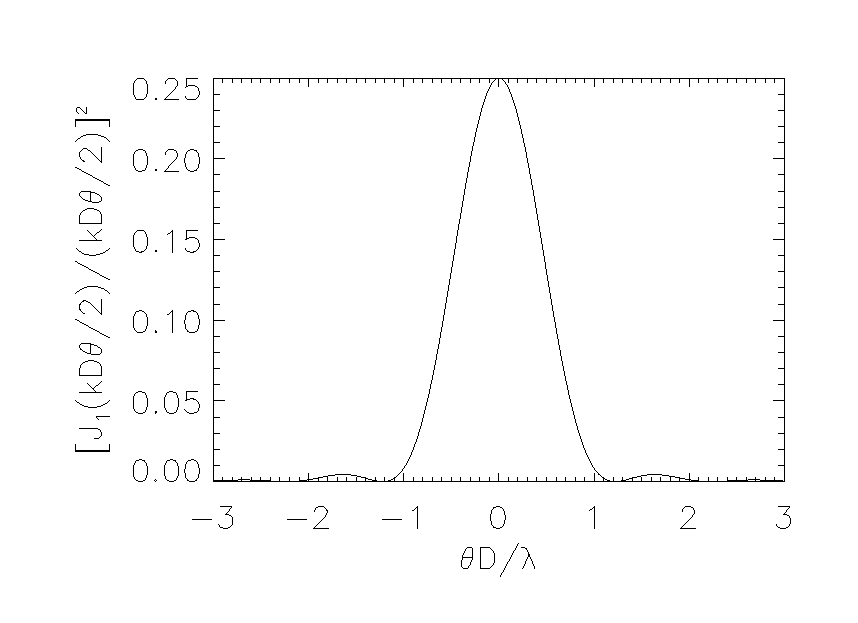
\psfig{file=jinc2.eps,width=0.7\textwidth}\hfil
	\centering
	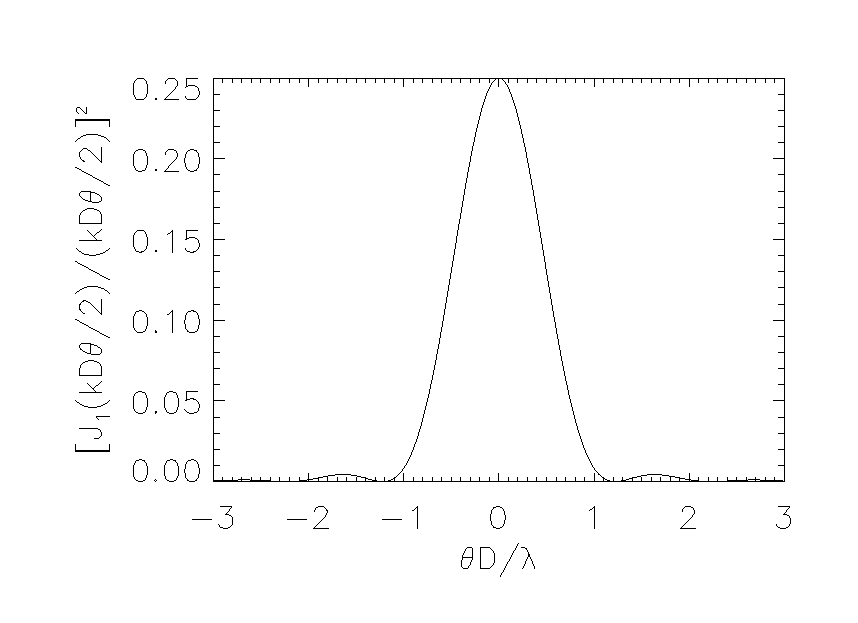
\includegraphics[width=0.7\textwidth]{jinc2.eps}
  \caption{Airy diffraction pattern for a circular aperture. Note the first zero
of the function at $\theta D/\lambda=1.22$.}
  \label{fig:jinc2}
\end{figure}

The calculation is straightforward using equation~\ref{eq:small-aperture} and assuming a circular
aperture telescope with diameter $D$:
\bua
\psi(\theta)&\propto&\int_{\pi D}e^{-ik{\bm x}\cdot{\bm\theta}}d^2x \\
            &\propto&{\rm jinc}\left({kD\theta\over 2}\right)
\eua
where ${\rm jinc}(x)\equiv {J_1(x)/x}$ with $J_1$ the Bessel function of order one. The
flux from an star observed at angle $\theta$ is therefore $\propto{\rm jinc}^2({kD\theta/2})$.
This intensity pattern is known as the {\it Airy pattern}. There is a central ``Airy disk'' 
surrounded by a circle where the flux vanishes, and then further surrounded by a series of 
concentric rings whose flux vanishes with radius. Only 16\% of the tatal light falls outside
the the central Airy disk. The angular radius $\theta_A$ of the Airy disk, {\it i.e.} the 
radius of the dark circle surrounding it, is determined by the first zero of 
$J_1({kD\theta/2})$ which is found to be $\theta_A={1.22\lambda/D}$. 

{\bf Exercise}

\begin{enumerate}
\setcounter{enumi}{\value{count}}
\item Write a {\tt IDL} routine that plots a cut through the Airy disk such as figure~\ref{fig:jinc2}
and, in addition, plots an image of the Airy disk.
\setcounter{count}{\value{enumi}}
\end{enumerate}

%\end{document}


% Lecture notes on Chapter 6:
\chapter{Telescopes for visible light}

Astronomers use telescopes to collect radiation from astronomical sources and
to estimate their direction and structure as well as spectral and absolute 
intensities. The wide range of photon energies involved in astronomical 
observations means that the telescopes are very different in form depending
on wavelength band. We can subdivide telescope types roughly into four 
categories. 
\begin{itemize}
\item detectors which sense the direction of arrival and energy of individual
(gamma-ray) photons
\item non-focusing (X-ray) collimators which restrict the field of view of 
the detector
\item phased arrays, and pencil beam interferometers (metre wavelength)
\item reflecting or refracting telescopes which focus incoming radiation 
(all wavelengths except gamma-rays)
\end{itemize}
Here we will concentrate on the latter category, and especially to those 
telescopes used to observe visible and infrared radiation. 
 
The theoretical
consideration of resolution that we discussed in previous lectures is only 
applicable if the lens or mirror as well as the intervening atmosphere
 is of sufficient optical quality that the image is not already degraded 
beyond the diffraction limit. There are many effects that will blur an image
and these are collectively known as aberrations. With one exception they 
can all effect images produced by both lenses or mirrors. The universal
or monochromatic aberrations are known as the Seidel aberrations. The 
exception is chromatic aberration and the related second order effects of 
transverse chromatic aberration and secondary color, and these only effect
lenses.

\section{Lenses, mirrors and geometric optics}

The speed of light in a vacuum is a constant, $c$, identical for all observers. 
The {\it phase velocity} $v$ of light in a dielectric medium such as air, water, or glass
is always less than $c$ such that
\[
n(\lambda)={c\over v(\lambda)}
\]
where $n$ is the {\it index of refraction}, which in general is a function of the 
wavelength $\lambda$. Another important characteristic of a material is thus the 
{\it chromatic dispersion} $dn/d\lambda$. Glassmakers traditionally express this
dispersion as the Abbe number, or costringence, defined in equation~\ref{eq:costringence}, 
which depends roughly on the reciprocal of the dispersion.

Along a ray of light moving through a medium (a homogenous medium will have straight rays
of light) one can measure the distance $s$ that light moves in time $t$
\[
s={ct\over n}
\]
Points of equal $s$ delineate a surface called the {\it geometrical wavefront}. Wavefronts
are always perpendicular to rays. If $ds$ is an infinitesimal element along a ray path the
ray travel time is 
\[
\tau=\int{ds\over v}={1\over c}\int nds={w\over c}
\]
where $w$ is the {\it optical path length}. In some situations with a coherent source (where
all waves are emitted in phase) the geometrical wavefronts also correspond to surfaces of
equal phase.

\subsection{Fermat's principle and Snell's law}

Fermat's principle states that the path of a ray between two points will always be an extremum
in total travel time $\tau$ or optical path length.

 Consider a situation where a plane separates
two different materials, and assume that the index of refraction is larger in the material on the
right. A light ray that travels towards the right will strike the normal to the surface at the 
{\it angle of incidence}, $\theta_1$, and the ray splits into two components - a reflected ray, 
and a refracted ray. These two rays make angles $\theta_R$ and $\theta_2$ with the normal, 
which is measured so that positive angles counterclockwise from the normal. 

Fermat's principle implies the law of reflection
\[
\theta_1=-\theta_R.
\]
We can also deduce the path of the refracted ray by requiring the optical path between two
fixed points $P_1$ and $P_2$ to be an extremum. This argument leads to Snell's law of 
refraction
\be
n_1\sin\theta_1=n_2\sin\theta_2
\label{eq:snell}
\ee
(Note that this expression reduces to the law of reflections for
$n_1=-n_2$.) 

For a ray coming
from a medium with a larger index of refraction there is a {\it critical angle} which 
produces a refracted ray that never leaves the medium, which one can see is given by 
\[
\theta_C=\sin^{-1}\left({n_1\over n_2}\right)
\]
This state of affairs is called a {\it total internal reflection}, where the angle of incidence is greater
than $\theta_C$, where all light that reaches the interface is reflected back into the higher index
medium. 

Snell's law is a general result that applies to any shape, and can be used as the foundation of 
almost all geometrical optics.

\subsection{Reflection and transmission coefficients}

The laws governing the relative {\it intensities} of incident and
reflected, refracted beams are complicated and fall outside the realm
of geometrical optics. {\it Fresnels formulas} for reflection and
transmission coefficients give the amplitudes of the reflected and
refracted waves as a function of angle of incidence, polarization, and
indices of refraction. A few results are worth stating:
\begin{itemize}
\item Polarization is important. Waves polarized with the electric
  field vector perpendicular to the plane of incidence (transverse
  electric phase), are reflected differently than waves polarized with
  the magnetic field perpendicular to the plane of incidence
  (transverse magnetic).
\item The reflectance, $R$, is the fraction of the power of the
  incident wave that is reflected. At normal incidence ($\theta_1=0$)
  and for all cases \[ R=\left({n_1-n_2\over n_1+n_2}\right)^2 \]
\item For both transverse electric and transverse magnetic
  polarization the reflectance becomes large at large angles of
  incidence. In the external case, $R\rightarrow 1.0$ as
  $\theta_1\rightarrow 90^{\circ}$ and light rays that strike a
  surface at grazing incidence close to $90^{\circ}$ will be mostly
  reflected. For the internal case, $R=1.0$ for all angles greater
  than the critical angle.
\item For all values of $\theta_1$ other than those described above
  $R$ is smaller for transverse magnetic than for transverse electric
  polarization. Thus initially unpolarized light become partially
  polarized after reflection from a dielectric surface. At one
  particular angle, {\it Brewster's angle} $\theta_{\rm
    p}=\tan{^{-1}({n_1/n_2})}$, $R=0$ for transverse magnetic
  polarization and only one polarization is reflected.
\end{itemize}

\begin{figure}[th]
	\centering
	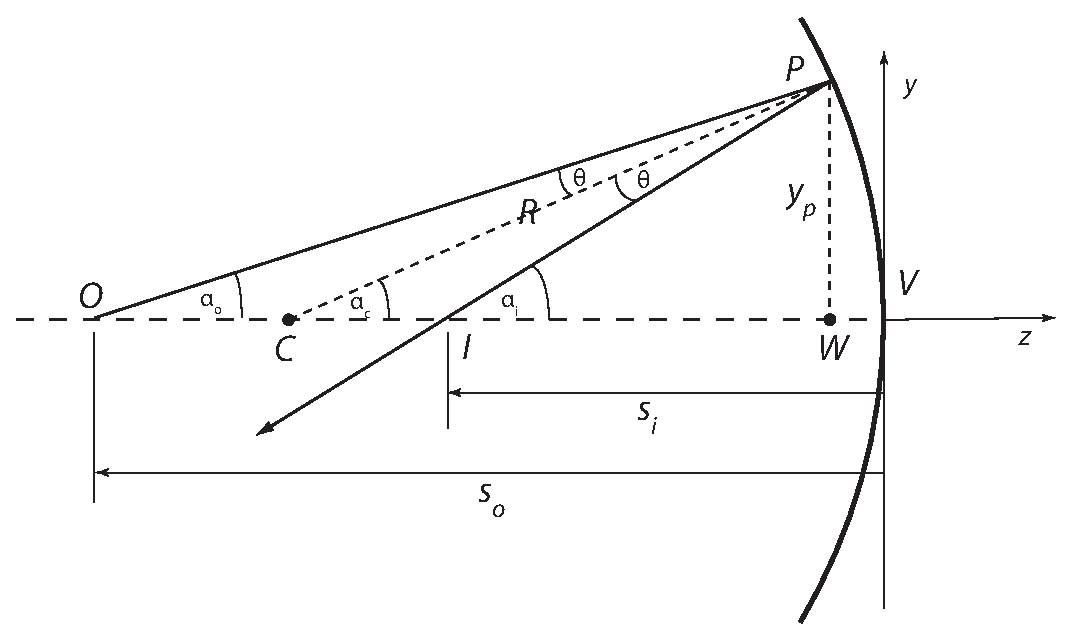
\includegraphics[width=0.9\textwidth]{reflection_spherical.eps}
  \caption{Reflection from a spherical surface. See text for details. }
  \label{fig:reflection_spherical}
\end{figure}

\subsection{Reflection from a spherical surface}

Consider a concave spherical surface with radius $R$ and center $C$ as
shown in figure~\ref{fig:reflection_spherical}. The line that is 
coincident with the axis of symmetry (goes through $C$ and the center of the surface)
is called the {\it optical axis}. Set up a Cartesian coordinate system where the $z$-axis
lies on the optical axis and the origin, the {\it vertex} ($V$) is at the point where the surface meets 
the optical axis. Let us describe the situation in the $y-z$ plane. The {\it paraxial approximation}
assumes that all incident rays are nearly parallel to the optical axis, and that all angles
of reflection are small. This latter means that the diameter of the mirror is small compared
to the radius of curvature. 

Consider the ray that originates at the {\it object} at point $O$ on the optical axis and is 
reflected at point $P$ to reach the image at $I$. If the point $P$ is at position $y_p$ then
we can deduce that 
\bua
\alpha_o&\approx&\tan\alpha_o\approx{y_p\over s_o} \\
\alpha_c&\approx&\tan\alpha_c\approx{y_p\over R} \\
\alpha_i&\approx&\tan\alpha_i\approx{y_p\over s_i} 
\eua
given that $s_o$ is the distance between the mirror surface and the object, and $s_i$ is the distance
between the image and the mirror surface (both along the optical axis). The angle $\alpha_c$ is the angle between the line joining the center of the surface $C$ and the point $P$ and the optical
axis.

If $\theta$ is the angle of incidence then we have, considering the triangles $OPC$ and $CPI$ 
that 
\[ 
\theta=\alpha_c-\alpha_o=\alpha_i-\alpha_c
\]
or
\[ 
2\alpha_c=\alpha_o+\alpha_i
\]
Substituting this into the first three approximations for the angles we derive
\[
{2\over R}={1\over s_o}+{1\over s_i}={1\over f}=-P.
\]
The distance $R/2$ is termed the {\it focal length} of the mirror, often written $f$, while
the {\it power} of the surface is written $P$. Note that as the object distance
$s_o$ goes to $\infty$ the image distance $s_i$ goes to $f$.

\subsection{Refraction in lenses} % Changed capital letter ``L'' in ``Lenses'' to 'l'.

Snell's law of refraction is also a good starting point for
understanding lenses.
Given that all angles are small, indicies of refraction $n_1,n_2$ and
a radius of curvature $R_{12}$, Snell's law implies that
\[
\frac{n_2}{s_2}-\frac{n_1}{s_1}=\frac{(n_2-n_1)}{R_{12}}.
\]
(note here that $s_1$ is negative).
If we take the focal length $f$ to be the value of $s_2$ when $s_1$
approaches infinity we have
\[
f_2=\frac{n_2R_{12}}{(n_2-n_1)}
\]
Thus, for refraction, the paraxial equation for image and object
distances is
\[
\frac{n_2}{s_2}-\frac{n_1}{s_1}=\frac{n_2}{f_2}=-\frac{n_1}{f_1}=P_{12}
\]
where $P_{12}$ is the {\it power} of the surface. The power, like the
focal length, measures how strongly converging (or diverging for
negative $P$) an interface is. A plane has zero power.

For a lens in air (or vacuum) we can set $n_1=1$ and $n_2=n$ giving the ratio of the speed of light
in vacuum/air to the speed of light in glass, {\it i.e.} $n={c/c_g}$. Snell's 
law implies that a plane wave front in vacuum/air remains plane as light 
enters the glass. A typical value for glass is $1.5$, so the speed of light 
in glass is some $200\,000$~km/s. Since the frequency of light does not change,
this means that the wavelength of light is shorter in glass than in vacuum.

An imaging lens is constructed so that the optical length $w$ in all rays is 
identical even if the geometric distances are different. 

\subsection{Imaging properties}

The relation between the distance from a thin lens to an object $s$ and to the 
image of the object $s'$ is related to the focal length $f$ of the lens by the 
thin lens formula
\[
{1\over s}+{1\over s'}={1\over f}
\]

Note that a point infinitely far away is imaged at the focal point of the 
lens, {\it i.e.} that for $s\rightarrow\infty$ then $s'=f$. 

Evaluating an optical design is best done by {\it ray tracing}, {\it
  i.e.} by tracing the path of several rays from an object through all
the optical elements until they form a final image. This is usually
done with a computer program that follows a number of rays, applying
Snell's laws and/or the laws of reflection at every interface ---
usually employing more exact formulations than the paraxial
approximation. However, using the paraxial approximation we can get a
(useful!) rough estimate using only a ruler, paper and a pencil. {\it
  Graphical ray tracing} uses the following specific rules for a thin lens:
\begin{enumerate}
\item Rays incident parallel to the axis emerge through the right
  focal point.
\item Rays incident through the left focal point emerge parallel to the
  axis.
\item Rays through the vertex do not change direction.
\end{enumerate}
Likewise, when dealing with a spherical mirror
\begin{enumerate}
\item Incident rays parallel to the optical axis are reflected through
  the focal point, $F$.
\item Incident rays through the focal point are reflected parallel to
  the axis.
\item Incident rays that reach the vertex are reflected back at an
  equal and opposite angle.
\item Incident rays through the center of curvature, $C$, are
  reflected back upon themselves.
\end{enumerate}

\subsection{Simple telescopes}

In its simplest form an astronomical telescope consists of two parts, an 
objective and an eyepiece. The objective images the object one is studying,
and which is ``infinitely'' far away (parallel rays in) on the focal point
or focal plane. This image is real, and can be seen if one places a screen 
in the focal plane. An eyepiece beyond the focal point functions as a 
magnifying glass. These two elements form the basic telescope (see figure~\ref{fig:telescope}).

\begin{figure}[th]
%  \hfil\psfig{file=telescope.eps,width=0.7\textwidth}\hfil
	\centering
	\includegraphics[width=0.7\textwidth]{telescope.eps}
  \caption{Schematic telescope design. Object has angular size $\alpha$ and is focused by 
the primary lens with focal length $F_1$. Image is observed using the eyepiece adjusted so
as to give a virtual image at infinity. The focal length of the eyepiece is $F_0$. }
  \label{fig:telescope}
\end{figure}

The {\it image scale}, $s$, describes the mapping of the sky by any camera. The image scale
is the angular distance on the sky that corresponds to a unit linear distance in the focal 
plane of the camera. Given a focal length $f$, draw paths followed by two rays, one from 
a point ({\it e.g.} a star) on the optical axis, the other from a point separated from the 
first by a small angle $\theta$ on the sky. Rays pass through the vertex without 
deviation, so assuming the paraxial approximation, $\theta\approx\tan\theta$, it is clear that
\[
s={\theta\over y}={1\over f}
\]
where $y$ is the distance the points are separated in the focal plane. Typical focal plane 
detectors are composed of many identical pixels. If the center of each pixel is separated 
from its nearest neighbors by $d$ then the {\it pixel scale} of a telescope is just $s_p=sd$.

The {\it focal ratio} is defined as 
\[
\cl{R}={f\over D}
\]
where $D$ is the diameter of the entrance aperture of the telescope. One can show that the 
brightness (energy per unit area to the focal plane) is proportional to $\cl{R}^2$.

The magnification $M$ of a telescope is given by considering that the image
formed by an object at an angle of $\alpha$ (assumed small) to the optical axis.
The real image is in focus at distance $F_1$, where $F_1$ is the focal length of the
objective lens, since the object is very far away. This image is observed by the eyepiece 
adjusted so as to give a virtual image at infinity, {\it i.e.} the eyepiece should be a distance
$F_0$ away from the image formed by the objective. Considering the geometry of the 
system shown in figure~\ref{fig:telescope} we see that the magnification $M$ must 
be given by $M={\beta/\alpha}$ and that therefore
\[ M={\beta\over\alpha}={\tan({h/F_0})\over\tan({h/F_1})}\approx{{h/F_0}\over{h/F_1}}={F_1\over F_0}.\]
Note that the image is formed upside down.

\section{Optical Materials}

An ideal mirror should have a reflectivity of 1.0 for all wavelengths ($\lambda$) of interest. The
substrate should be easy to shape to an accuracy of a fraction of $\lambda$, and once shaped, 
should be mechanically and chemically stable. Low mass is a virtue, as mirrors and lenses should
be as large as possible and must be mobile. Since the temperature can change rapidly high 
thermal conductivity and a low coefficient fo thermal expansion are also essential.

For reflecting telescope's first two centuries, one used {\it speculum metal}, an alloy
primarily of copper and tin. However, it was (is) heavy and only has 45\% reflectivity at best, 
and tarnishes easily. Astronomers therefore switched to silvered glass mirrors once the 
technology became available in the 1880s. Most modern mirrors generally use substrates
made with special glasses ({\it e.g.} Pyrex) or ceramics (Cervit or Zerodur) that have low
coefficients of thermal expansion. A coating of Al is best for the near ultraviolet and optical
since Al is durable and cheap. Ag is poor in the ultraviolet, is superior to Al when 
$\lambda>450$~nm. Au is best in the infrared for $\lambda>650$~nm. Be is toxic, but is the
lowest density workable metal with very good rigidity. 

Short wavelengths, extreme ultraviolet (EUV) and shorter, present
difficulties: First energetic photons tend to be absorbed, scattered,
or transmitted by most materials, and second, curved mirrors in general
need to be shaped with an accuracy of at least $\lambda/4$, which for
a 1~nm X-ray, amounts to one atomic diameter! X-Ray and EUV focusing
telescopes are therefore often designed to operate with grazing
incidence as discussed later.

Transmitting materials form lenses, windows, correctors, prisms, filters, fibres, and more. Of
primary relevance are index of refraction, dispersion, and absorption. The index of refraction for
a number of glasses as a function of wavelength $\lambda$ is shown in table~\ref{tab:glass-refraction}. Generally glasses with a high index of refraction will also have high dispersion and are called ``flints'', while those with smaller index and dispersion are 
called ``crowns''. 

In ultraviolet (150~nm -- 400~nm) ordinary glasses become opaque, fused quartz (SiO$_2$) is
the exception. All other ultraviolet transmitting materials are crystalline, rather than glass, and
are more difficult to shape and more likely to chip and scratch. The most useful is perhaps
calcium fluoride (CaF$_2$), which transmits from 160~nm to 7~$\mu$m. Other fluoride crystals
have similar properties. Fused quartz and fluorides do not transmit well below 180~nm and some
birefringent crystals, such as sapphire (Al$_2$O$_3$) can be used in the very far ultraviolet.
Optics for $\lambda < 150$~nm must be reflecting and for $\lambda < 15$~nm only grazing
incidence reflections are possible.

In the infrared ordinary glasses transmit to about $2.2~\mu$m, and some special glasses to 
$2.7~\mu$m. A large selection of crystalline materials, some identical to those used in the
ultraviolet, transmit to much longer $\lambda$, but most are soft, or fragile, or sensitive to
humidity, so can only be used in protected environments.

% Maybe change table width to fill the textwidth.
\begin{table}
\centering
\begin{tabular*}{\textwidth}{p{0.3\textwidth}@{\extracolsep{\fill}}p{0.1\textwidth}p{0.1\textwidth}p{0.1\textwidth}p{0.1\textwidth}p{0.1\textwidth}}
%\begin{tabular*}{\textwidth}{l@{\extracolsep{\fill}}lllll}
\toprule
\toprule
%& & & & & \\
& \multicolumn{5}{c}{Refractive index at the specified wavelengths (nm)} \\
\cmidrule{2-6}
Glass type & 361 & 486 & 589 & 656 & 768  \\
\midrule
%& & & & & \\
Crown & 1.539 & 1.523 & 1.517 & 1.514 & 1.511 \\
High dispersion crown & 1.546 & 1.527 & 1.520 & 1.517 & 1.514 \\
Light flint & 1.614 & 1.585 & 1.575 & 1.571 & 1.567 \\
Dense flint & 1.705 & 1.664 & 1.650 & 1.644 & 1.638 \\
\bottomrule
\bottomrule
\end{tabular*}
\caption{Index of refraction in various glass types vary as a function
of wavelength and are thus dispersive.}
\label{tab:glass-refraction}
\end{table}

Coating the surface of an optical element with a thin film can exploit
the wave properties of light to increase, or decrease, its
reflectance. A thin film exactly ${1/4}$ wavelength thick applied to a
reflecting substrate will introduce two reflected beams, one from the front film
surface, and the other from film-substrate interface. The second beam
will be emerge one-half wavelength out of phase, and the two beams
will destructively interfere. If the amplitudes are equal, the
interference will be total. An antireflection coating works best at only
one wavelength, but will to some extent also work for a broader band
centered near the design wavelength. A similar technique can enhance
the reflectivity of a surface and multiple layers fo alternating high
and low index materials can improve the reflectivity of a mirror over
a broad range of mirrors. Such {\it multilayer mirrors} are in
frequent use in solar satellites observing the sun at normal incidence
in the EUV as will be discussed later.

\section{Chromatic aberration}

Chromatic aberration arises through the change in the refractive index of
glass or other optical material with the wavelength. Typical values for
some optical glasses are shown in table~\ref{tab:glass-refraction}. The 
degree to which the refractive index varies with wavelength is called the 
dispersion, and is measured by the constringence $\nu$
\begin{equation}
\nu={\mu_{589}-1\over\mu_{486}-\mu_{656}}\label{eq:costringence}
\end{equation}
where $\mu_\lambda$ is the refractive index of the wavelength $\lambda$. Note
that the costringence (also called the {\it Abbe number} is roughly inversely 
proportional to the dispersion, {\it i.e} $({dn/d\lambda})$.  The
three wavelengths that are chosen for the definition of $\nu$ are those
of strong Fraunhofer lines: the C-line 486~nm H$\beta$, the D lines 589~nm (Na), 
and the F-line 656~nm H$\alpha$. The glasses listed above have constringence that 
varies from 57 for crown glass to 33 for the dense flint. 

\begin{figure}[th!]
 \centering
 \includegraphics[width=0.5\textwidth]{chromatic-aberration.eps}
  \caption{Chromatic aberration.}
  \label{fig:chromatic-aberration}
\end{figure}

The effect of dispersion upon an image is to spread it out into a series of
different colored images along the optical axis. Looking at this sequence of
 images with an eyepiece, then at a particular point along the optical axis, the
observed image will consist of a sharp image in the light of one wavelength
surrounded by blurred images of varying sizes in the light of all remaining 
wavelengths. To the eye, the best image occurs when yellow light is focused 
since it is less sensitive to red and blue light.
The spread of colors along the optical axis is called the
{\it longitudinal chromatic aberration}, while that along the image plane
containing the circle of least confusion is called the {\it transverse
chromatic aberration}.

\begin{figure}[th!]
	\centering
	\includegraphics[width=0.9\textwidth]{sst-design.eps}
  \caption{Schematic drawing of the Swedish 1-meter Solar Telescope tower 
with the turret and vacuum system (center drawing). Details of the box 
holding the field mirror and field lens are shown in A and the Schupmann 
corrector with one lens and one mirror in B. The re-imaging optics, located on
the optical table and consisting of a tip-tilt mirror, an adaptive mirror 
and a re-imaging lens are shown in C.}
  \label{fig:sst-design}
\end{figure}

Delayed by Newton's declaration of impossibility, in the 1760s in France 
and England it was discovered that 
two (or more) lenses can be combined to reduce the effect of chromatic 
aberration. Commonly a biconvex crown glass lens is combined with a 
planoconcave flint glass lens to produce an {\it achromatic doublet}. This can 
reduce the chromatic dispersion by a factor 30. If the radii of the 
curved surfaces are all equal, then the condition for two wavelengths,
$\lambda_1$ and $\lambda_2$, to have coincident images is 
\[
2\Delta\mu_C=\Delta\mu_F
\]
where $\Delta\mu_C$ and $\Delta\mu_F$ are the differences between the 
refractive indices at $\lambda_1$ and $\lambda_2$ for the crown glass and
flint glass respectively. More flexibility in the design can be achieved 
if the two surfaces of the converging lens have differing radii. Then the
condition for achromatism is
\[
{\labs R_1\rabs+\labs R_2\rabs\over\labs R_1\labs}\Delta\mu_C=\Delta\mu_F
\]
where $R_2$ is the radius of the surface of the crown glass that is in 
contact with the flint lens and $R_1$ is the radius of the other surface
of the crown glass lens. Fraunhofer perfected the design and construction
of achromats which led to the possibility of making large refractors, which became 
the telescope design of choice at most observatories after the 1820s.
The era of the refractor came to an end around 1900 when the size of these
reached roughly 1~m, above which size gravity deforms the shape of the lens. It is 
interesting to note that the Swedish 1-meter Solar Telscope with a 1.0~m lens is
one of the worlds largest refractors.

Since photographic film has a different wavelength sensitivity than the
human eye, achromats had to be redesigned when photographic technology 
was adopted by astronomers in the 1880s. 

It is possible to design doublets so that three or more wavelengths are corrected, in this
case the corrective lenses are called {\it apochromats}. Adding more lenses, a properly 
designed {\it triplet}, called a {\it superapochromat} can bring four wavelengths into 
a common focus.

\subsection{Schupmann achromat}

Another interesting solution to the problem of achieving an achromatic image
is the combination of a positive lens and a second negative lens in which case
one has an intermediate image and the final image is virtual. This is named
a Schupmann lens. The drawback of the virtual image location can be overcome
with the help of a mirror. The collecting mirror is placed behind the negative
lens, which is used twice and therefore has less power than the negative lens
in the usual setup. There are few refracting telescopes in professional night 
time astronomy, but the Swedish 1-meter Solar Telescope is a refracting 
telescope in which a Schupmann achromat is used.

\section{Seidel Aberrations}

\begin{figure}[th!]
	\centering
	\includegraphics[width=0.95\textwidth]{aberration_geometry.eps}
  \caption{Geometry used in the Seidel aberration discussion. The left hand
diagram shows rays through the the center of curvature (CFB) and vertex (VV', the chief ray), which
along with the optical axis defines the meridional plane. Point P is outside the plane of the diagram. 
The right hand locates points P, V, and B in the plane of the aperture when looking down the optical axis.}
  \label{fig:aberration-geometry}
\end{figure}

Consider a ``perfect'' telescope, it should transform an incident plane wavefront into
a converging spherical wavefront whose center is the focus predicted by the paraxial 
approximation. For point sources off-axis the perfect telscope should produce spherical
wavefronts converging somewhere on the image plane, also as predicted by the paraxial 
theory. Define the {\it chief ray} as the one passing from the object through the center
of the entrance aperture. The plane containing this ray and the optical axis defines the
{\it meridional} or {\it tangential plane}. The plane perpendicular to this plane is called
the {\it sagittal plane}. If we now analyse the angles of reflection or refraction for a 
curved surface using the approximation 
\[
\sin\theta\approx\theta-{\theta^3\over 3!}
\] 
one obtains {\it third-order aberration theory} which is much more accurate than that
given by paraxial theory where one assumes $\sin\theta=\tan\theta=\theta$. In this 
treatment one can show that the optical path {\it difference} between a test ray and the
chief ray takes the form
\bea{eq:seidel}
\Delta w(\rho,\phi,b)&=&C_1\rho^4+C_2\rho^3b\cos\phi \\
                                &+&C_3\rho^2b^2\cos^2\phi+C_4\rho^2b^2+C_5\rho b^3\cos\phi
\eea
where the $C_i$ values depend on the shapes of the optical surfaces and/or the indices of
refraction. Each of the terms in this equation~\ref{eq:seidel} has a different functional
dependence, so one distinguishes five monochromatic third-order aberrations which are
also known as the {\it Seidel aberrations}. Note that since the range of $\rho$ depends on 
the diameter of the telescope the terms with the highest order of $\rho$ are the most
important.

\subsection{Spherical aberration $\propto\rho^4$}

\begin{figure}[th!]
	\centering
	\includegraphics[width=0.9\textwidth]{spherical-aberration.eps}
  \caption{Spherical aberration.}
  \label{fig:spherical-aberration}
\end{figure}

A common and severe aberration of both lenses and mirrors is {\it spherical 
aberration}: annuli of the lens or mirror that are of different radii have 
different focal lengths. It is possible to minimize but not eliminate spherical
aberration by minimizing the angles of incidence on every surface. Likewise,
any lens with a large enough focal ratio will approach the paraxial case closely enough
that the blur due to spherical aberration can be made smaller than the seeing disk.
Since a large focal ratio also minimizes the chromatic aberration, early refracting telescopes 
(1608 -- 1670) tended to have moderate apertures and large focal lengths, at the cost
of reduced image brightness and unwieldy telescope length.

For mirrors, removing spherical aberration is simple. A paraboloid reflector, 
made by deepening the sphere to a paraboloidal surface, 
will display no on-axis aberrations at all --- rays from infinity parallel to 
the axis will all come to the same focus. Newton constructed the first 
workable reflecting telescope in 1668, and reflecting
telescopes were fashionable from the 1780s (when the Herschels were making great
discoveries with speculum parabaloids) until the superiority of the refractor became
apparent in the 1830s as a result of the discovery that an achromatic doublet can be 
designed to minimize both chromatic aberration and spherical aberration:  
These cannot be
eliminated from a simple lens without using aspheric surfaces, but can be
reduced for a given focal length by adjusting the shape factor $q$
\[
q={R_2+R_1\over R_2-R_1}
\]
where $R_1$ and $R_2$ are the radii of the first and second surfaces 
of the lens respectively. Judicious choice of surface radii in an 
achromatic doublet can lead to some correction of spherical aberration while
still retaining the color correction. 

It is also possible to remove spherical aberration from a {\it spherical} mirror by 
the use of a transparent corrector plate, as we will discuss in connection with
Schmidt and Maksutov telescopes later in this lecture.

%Spherical aberration increases with
%the fourth power of the diameter and inversly proportional to the third 
%power of the focal length.

\subsection{Coma $\propto \rho^3b\cos\phi$}

{\it Coma} in an optical system refers to an aberration which results
in off-axis point sources such as stars appearing distorted. Specifically, 
coma is defined as a variation in magnification over the entrance pupil. 
Coma is an inherent property of telescopes using parabolic mirrors, thus
deepening a spherical mirror in order to correct spherical aberration will
introduce coma. It causes the images for objects away from the optical axis
to consist of a series circles that correspond to the various annular 
zones of the lens or mirror and which are progressively shifted away from 
the optical axis. The severity of the coma is proportional to the square of
the aperture and the angular size of the blur is given by
\[ 
L=A{bD^2\over f^3}=A\theta\cl{R}^{-2}
\]
where $A$ is a constant that depends on the shape of the surface.

% Coma is zero in systems that obey Abbe's sine condition
%\[
%{sin\theta\over\sin\phi}={\sin\theta_{\rm p}\over\sin\phi_{\rm
%    p}}\approx{theta_{\rm p}\over\phi_{\rm p}}
%\]
%where the angles are de$\theta$, $\phi$ are the angles relative the optical axis
%of any two rays as they leave the optical system and $\theta_$, $\phi'$ the
%angles of the same rays as they reach the image plane. In other words, 
%the sine of the output angle should be proportional to the sine of the 
%input angle in order to satisfy Abbe's sine condition.

%\begin{figure}[th!]
%  \hfil\psfig{file=abbes-sin.eps,width=0.9\textwidth}\hfil
%  \caption{Angles used in describing Abbe's sine condition.}
%  \label{fig:abbes-sin}
%\end{figure}

Lenses or mirrors in which both spherical aberration and coma are minimized at a single
wavelength are called best form or {\it aplanatic}. No single element aplanatic telescope
is possible, either in a reflector or a refractor. As with spherical aberration, a large
focal ratio will reduce coma, but impose penalties in image brightness and telescope length.
Otherwise, minimizing coma in a refracting system requires a system of lenses, and at least
two mirrors in reflecting telescopes.

\subsection{Astigmatism $\propto b^2\rho^2\cos^2\phi$}

\begin{figure}[th!]
%  \hfil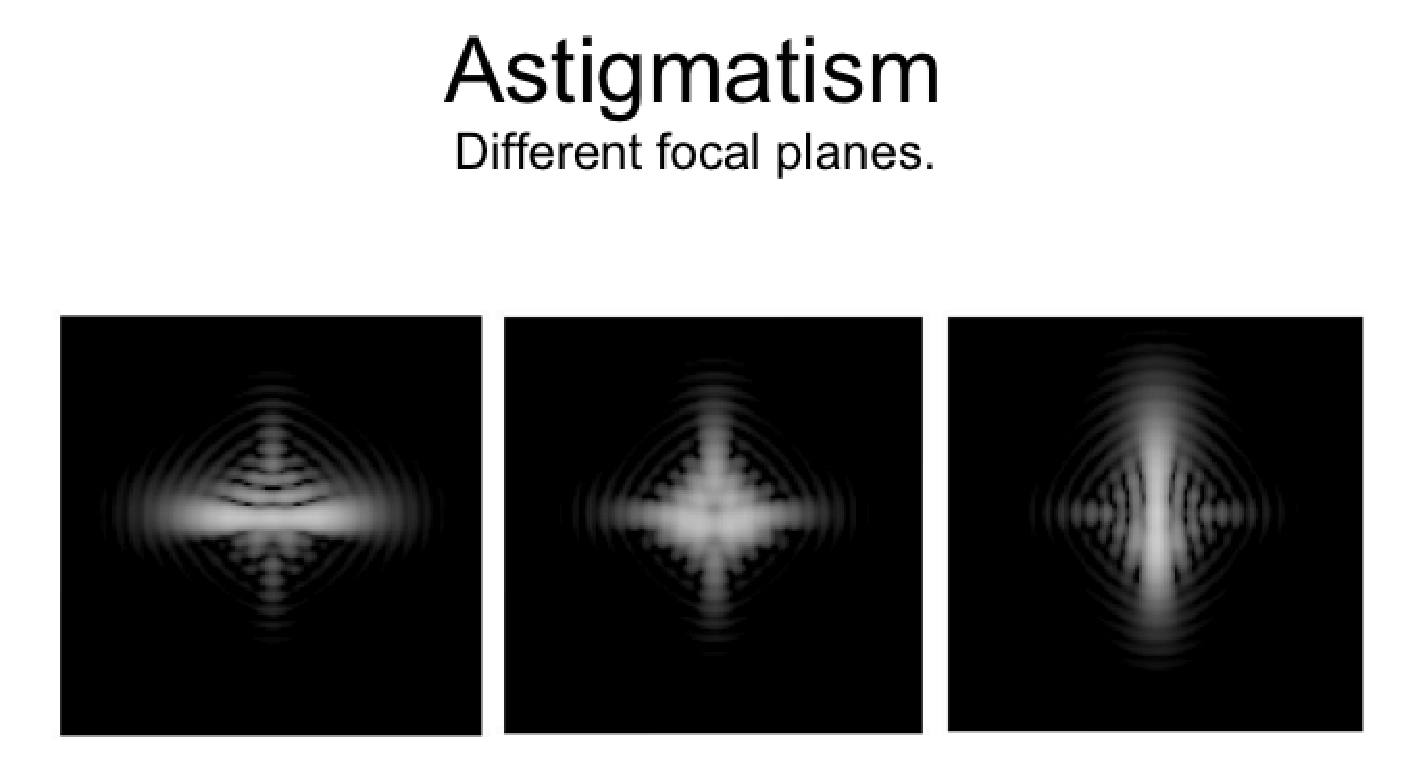
\psfig{file=astigmatism-example.eps,width=0.7\textwidth}\hfil
	\centering
	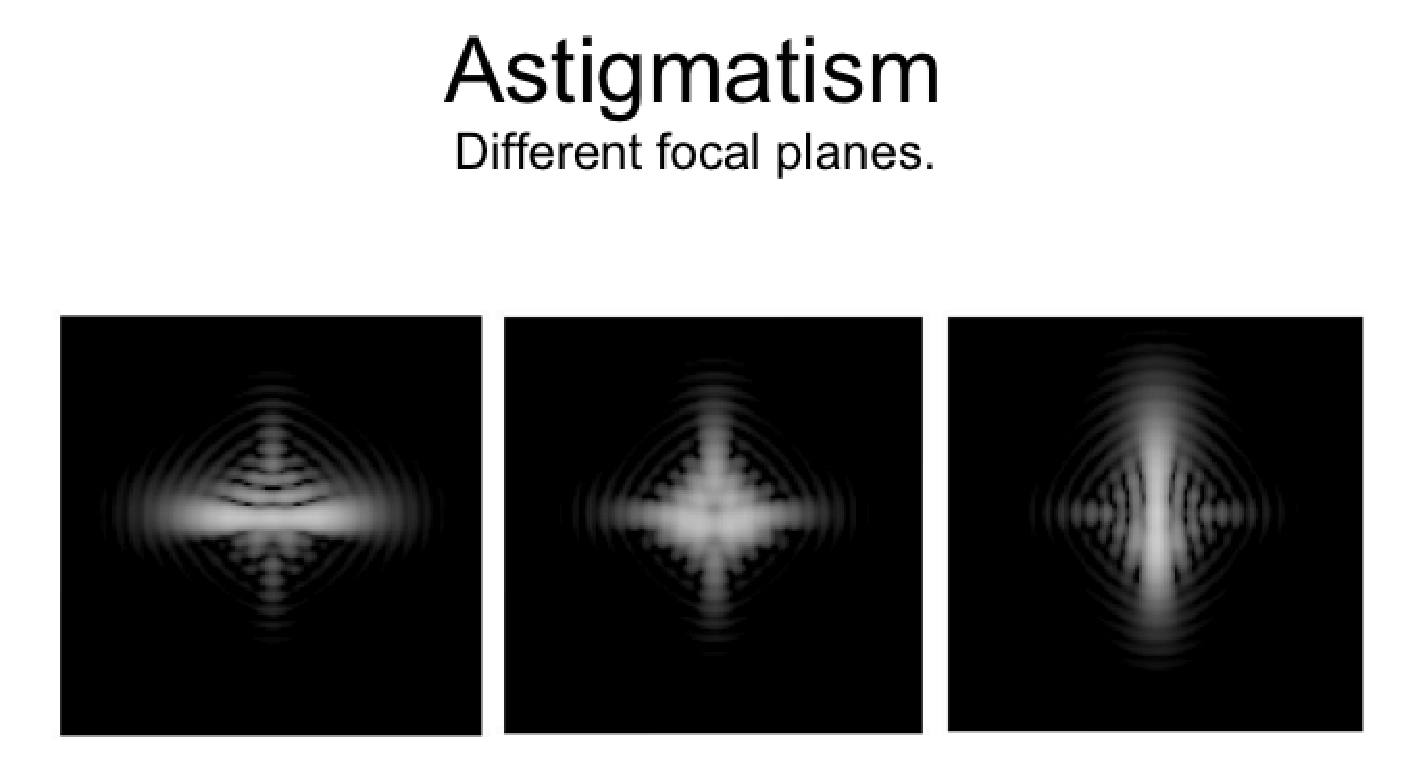
\includegraphics[width=0.7\textwidth]{astigmatism-example.eps}
  \caption{Example of the effect of astigmatism.}
  \label{fig:astigmatism-example}
\end{figure}

{\it Astigmatism} is an effect where the focal length differs for rays in the plane
containing an off-axis object and the optical axis (tangential plane),
in comparison with rays in the plane at right angles to this (sagittal plane).
An example of astigmatism is shown in figure~\ref{fig:astigmatism-example}.
The angular dependence suggests that the wavefront distortion is zero for rays
in the sagittal plane ({\it i.e.} $\phi=90^{\circ}$, $\phi=270^{\circ}$), but an extremum for
rays in the meridional plane.

The blurred image suffering astigmatism has an angular length
\[
L=B\theta^2\cl{R}^{-1}
\]
where $B$ is a constant that depends on the shape of the reflecting or refracting surface.

It is possible to correct astigmatism, but at the expense of introducing
an aberration called field curvature, {\it i.e.} that the surfaced containing
the sharply focused image is not flat but curved. A system where a flat 
image plane is combined with corrected astigmatism is termed {\it anastigmatic}
and a telescope that corrects for astigmatism, coma, and spherical aberration a
anastigmatic aplanat. 

\subsection{Field curvature $\propto\rho^2 b^2$}

This aberration results from off-axis images falling on a spherical surface called the
{\it Petzval surface}. Detectors are generally flat, so much of an image formed on a 
detector will be out of focus. For a small detector, this defocus will not exceed the 
seeing disk or diffraction limit and therefore not be a problem. For larger detectors
is to bend the detector to fit the Petzvel surface, as was done with photographic plates
using a mechanical plate holder. Large solid-state detectors like CCDs are mechanically 
quite fragile, so bending is not an option. In which case a corrector plate or lens is
used to flatten the field.

\subsection{Distortion $\propto \rho b^3\cos\phi$}

\begin{figure}[th!]
	\centering
	\includegraphics[width=0.9\textwidth]{aberration-distort.eps}
  \caption{Distortion}
  \label{fig:aberration-distortion}
\end{figure}

The final aberration is {\it distortion}, which is a variation in the 
magnification over the image plane. A distorted system will deliver images
that suffer {\it pincushion} or {\it barrel} distortion according to 
whether the magnification increases or decreases with distance from the 
optical axis.

Since distortion does not change the image quality, it can be removed from 
digital in a post processing phase.

Another fault of optical systems is called {\it vignetting}. It arises as a result
of uneven illumination of the image plane, usually due to the obstruction of 
the light path by parts of the instrument.

\subsection{Zernike polynomials}

\begin{figure}[th!]
	\centering
	\includegraphics[width=0.4\textwidth]{zernike_polynomials.eps}
  \caption{The first few Zernike polynomials, see table~\ref{tab:zernike-polynomials} 
}
 \label{fig:zernike-polynomials}
\end{figure}

\begin{table}
	\centering
	\begin{tabular*}{\textwidth}{p{0.25\textwidth}@{\extracolsep{\fill}}p{0.70\textwidth}}
\toprule
\toprule
Zernike polynomials & Roles of the Zernike polynomials \\ 
\midrule
$a_0$ & ``Piston'', equal to the mean value of the wavefront \\
$a_1\times\rho\cos(\varphi)$ & ``X-tilt'', deviation of the overall beam in the sagittal direction \\
$a_2\times\rho\sin(\varphi)$ & ``Y-tilt'', deviation of the overall beam in the tangential direction \\
$a_3\times(2\rho^2-1)$ & ``Defocus'', a parabolic wavefront resulting from being out of focus \\
$a_4\times\rho^2\cos(2\varphi)$ & ``X-astigmatism'', horizontally oriented cylindrical shape \\
$a_5\times\rho^2\sin(2\varphi)$ & ``Y-astigmatism'', vertically oriented cylindrical shape \\
$a_6\times(3\rho^2-2)\rho\cos(\varphi)$ & ``X-coma'', comatic image flaring in the horizontal direction \\
$a_7\times(3\rho^2-2)\rho\sin(\varphi)$ & ``Y-coma'', comatic image flaring in the vertical direction \\
$a_8\times(6\rho^4-6\rho^2+1)$ & ``Third order spherical aberration'' \\
\bottomrule
\bottomrule
\end{tabular*}
\caption
{$\rho$ is the normalized pupil radius, $\varphi$ is the azimuthal angle around the pupil,
the coefficient $a_0,\ldots,a_8$ are the wavefront errors in wavelengths.}
\label{tab:zernike-polynomials}
\end{table}

In an optical system the location of the diffraction focus will depend
on the type and magnitude of aberration present. Because of this
dependence, it is appropriate to restructure the classical aberration
terms and include explicitly the required image shift to place the
diffraction focus at the origin. These modified terms are called the
orthogonal aberrations, with polynomials in $\rho$ and $\varphi$ ({\it
  i.e.} using a circular co-ordinate system) called
{\it Zernike polynomials}. Developed by Frits Zernike in the 1930s,
 Zernike's polynomials are orthogonal over a circle of unit radius. A complex, 
aberrated wavefront profile may be curve-fitted with Zernike polynomials to 
yield a set of fitting coefficients that individually represent different 
types of aberrations. Their advantage are the simple analytical
properties which leads to closed form expressions of the
two-dimensional Fourier transform in terms of Bessel functions. 
Their disadvantage, in particular for high $n$ is the unequal
distribution of nodal lines over the unit disk, which introduces
ringing effects near the perimeter $\rho\approx 1$, which leads
attempts to define other orthogonal functions over the circular 
disk\footnote{For atmospheric turbulence
  Zernike polynomials are not the optimal set of basis functions
  because the Zernike coefficients are statistically dependent. Basis
  functions that do not have this property can be constructed and are
  called the {\it Karhunen--Lo{\'e}ve functions} which represent
stochastic processes as an infinite linear combination of orthogonal
functions analogous to a Fourier series representation of a function
on a bounded interval. The coefficients in the Karhunen--Lo{\'e}ve
theorem are random variables and the expansion basis depends on the
process. The Karhunen--Lo{\'e}ve transform adapts to the process in 
order to produce the best possible basis for its expansion. (Source: 
Wikipedia and Gua-ming Dai {\it Modal compensation of atmospheric
  turbulence with the use of Zernike polynomials and
  Karhunen-Lo{\'e}ve functions} J.Opt.Soc.Am. 12, October 1995.)}.

There are even and odd Zernike polynomials. The even ones are defined as
\[
Z_n^m(\rho,\varphi)=R_n^m(\rho)\cos(m\varphi)
\]
and the odd ones
\[
Z_n^{-m}(\rho,\varphi)=R_n^m(\rho)\sin(m\varphi)
\]
where $m$ and $n$ are non-negative integers with $n\ge m$, $\varphi$ is the
azimuthal angle and $\rho$ is the normalized radial distance. The radial 
polynomials $R_n^m$ are defined as
\[
R_n^m(\rho)=\sum_{k=0}^{(n-m)/2}{(-1)^k(n-k)!\over 
   k![{(n+m)/2}-k]![{(n-m)/2}-k]!}\rho^{n-2k}\qquad{\rm if}~n-m~{\rm even}
\]
\[
R_n^m(\rho)=0\qquad{\rm if}~n-m~{\rm odd}
\]

The first few few Zernike polynomials are described in table~\ref{tab:zernike-polynomials}.

\section{Practical telescopes}

Even after a telescope design has been perfected; in which one attempts to 
remove as many of the aberrations as possible from the list above, there 
remains the task of physically producing the instrument specified. This must
be done taking into consideration what one actually needs to observe in 
order to meet a certain scientific goals. 

Manufacturing of lenses and mirrors is broadly similar: the surface is roughly
shaped by moulding or diamond milling. It is then matched to another surface
formed in the same material whose shape is inverse, called the {\it tool}. 
The two surfaces are ground together with coarse carborundum or other grinding
powder between them until the required surface begins to approach 
its specifications. The pits left behind are removed by a second grinding stage
in which finer powder is used. A third stage follows, and so on. As many as
eight or ten such stages may be necessary. When grinding pits are reduced to
a micron or so in size, the surface may be polished. Once the surface has been
polished it can be tested for accuracy of fit. A third stage termed {\it 
figuring} is often necessary when the surface is not within specification. 

There are a number of tests that can determine the shape of a mirror's surface
to within $\pm 50$~nm or better, such as Foucault, Ronchi, Hartmann and Null
tests. 

\noindent
{\bf Epicyclic grinding.} Larger mirrors are ground by using large machines that 
move the tool in an epicyclic fashion. The motion of the tool is similar to that of 
the planets under the Ptolemaic model of the solar system. The epicyclic motion 
can be produced by a mechanical arrangement, but commercial production of 
large mirrors is now largely done by computer controlled planetary polishers. 

\noindent
{\bf Stressed polishing.} The mirror segments for large instruments such as the 10~m
Keck or Gran Tecan telescopes are small, off-axis parts of the total hyperbolic shape. 
These are produced by so-called stressed polishing where the blank is is deformed 
by carefully designed forces from a warping harness, and then polished to a spherical
shape. When the the deforming forces are released the blank springs into the required 
shape.

\noindent
{\bf Numerically controlled diamond milling.} The requirements for for non-axisymmetric
mirrors for segmented mirror telescopes and and for glancing incidence x-ray telescopes
have led to the development of numerically controlled diamond milling machines which 
can produce the required shaped and polished surface directly to an accuracy of 10~nm or
better.

The defects in an image that are due to surface imperfections on a mirror will
not exceed the Rayleigh limit if those imperfections are less than 
one eighth of the wavelength of the radiation for which the mirror is intended.
The restriction on lenses is about twice as large as those of a mirror
since the ray deflection is distributed over two faces. 

The surface must normally receive its reflecting coating after production. The
vast majority of astronomical mirror surfaces have a thin layer of aluminium
evaporated on to them by heating aluminium wires suspended over the mirror 
inside a vacuum chamber. Other materials such a silicon carbide are sometimes
used, especially for UV since the reflectivity of aluminium falls for 
$<300$~nm. Aluminium initially has a reflectivity of 90~\%, but this will
fall to 75~\% in the matter of months, hence realuminaization is need 
regularly. Mirrors coated with suitably protected silver can achieve 99.9~\%
reflectivity in the visible, and this may be required as the total number of
reflections becomes large.

\noindent
{\bf Coefficient of thermal expansion.} To avoid deformations of its shape it is essential
that the coefficient of thermal expansion for a mirror is low. For glass it is of order
$9\times 10^{-6}$~K${-1}$, for pyrex $3\times 10^{-6}$~K${-1}$, and for fused quartz
$4\times 10^{-7}$~K${-1}$. Pyrex has been the favorite material up until the last 30 years
when quartz or artificial materials such as `CerVit' or `Zerodur'. Another possibility is to 
use materials with a very high thermal conductivity, such as silicon carbide, graphite epoxy,
steel beryllium, or aluminium. However, it can be very difficult to polish these materials as
they have a relatively coarse crystalline surface.

\noindent
{\bf Rigidity of mirrors, thin mirrors and honeycomb mirrors.} Small solid mirrors can maintain
their shape simply by mechanical rigidity. However, the thickness required for such rigidity
scales as the cube of the size, so the weight of a solid mirror scales as $D^5$ --- this quickly 
becomes to expensive to build. There are various ways to reduce the weight of mirrors, these
fall into two major classes: thin mirrors and honeycomb mirrors. Thin mirrors are also subdivided
into monolithic and segmented mirrors. In both cases active support is needed in order to 
maintain the correct shape. Honeycomb mirrors are thick sold blanks that have had a lot of
the material behind the reflecting surface removed, leaving only thin struts to support that surface. 

\noindent
{\bf Rotating mirrors, bath of mercury.} Isaac Newton realized that the surface of a steadily rotating liquid would take up a paraboloidal shape under the combined forces of gravity and
centrifugal acceleration. If the liquid reflects light, like mercury, gallium, gallium-indium alloy, or an oil suffused with reflecting particles, one can then use it as the primary mirror of a telescope. 

\subsection{Designs}

\subsubsection{Cassegrain}
The most common format for large telescopes is the Cassegrain system, although
most large telescopes can usually be used in several alternative 
modes by interchanging the secondary mirrors. The Cassegrain system is
based on a paraboloidal primary and a convex hyperboloidal secondary mirror.
The light reflects off of the primary mirror and converge to its focal point (focus).
Before the reflected light meet at the focus, it is instead redirected by the
secondary mirror, so that the light rays instead
converge to the secondary focus which is usually behind the primary mirror. The light passes 
through a hole in the primary mirror, where it is detected by e.g. a CCD at the secondary
focus.
The major advantage of the Cassegrain lies in its telephoto characteristic, 
the secondary mirror serves to expand the beam from the primary mirror so 
that the effective focal length of the whole system is several times the
that of the primary. A compact (thus cheap) mounting can thus be used to 
hold the optical elements while retaining the advantages of long focal length
and large image scale. The Cassegrain is affiliated with coma and spherical
aberration to about the same degree as an equivalent Newtonian.

\begin{figure}[th!]
	\centering
	\includegraphics[width=0.45\textwidth]{cassegraindetailed.eps}
	\includegraphics[width=0.45\textwidth]{newtoniandetailed.eps}
  \caption{Cassegrain (left) and Newtonian (right) designs}
  \label{fig:catatropic}
\end{figure}

\subsubsection{Ritchey-Chr\'{e}tien}
A great improvement of the Cassegrain is the Ritchey-Chr{\'e}tien system.
The optical arrangement is identical, but the
primary mirror is deepened to a hyperboloid and a stronger 
hyperboloid is used for the secondary. This is done to correct for both coma and 
spherical aberration so that one achieves an aplanatic system. 

\subsubsection{Corrector lenses just before the focus}
One can also improve Cassegrain
or Ritchey-Chr\'etien systems by adding correctors just before the focus. 
The correctors are low power lenses whose aberrations oppose those of the main
system. The corrective optics may be combined with a focal reducer to enable 
the increased field of view to by covered by the detector array. A focal reducer
is a positive lens, usually a apochromatic triplet, placed just before the focal 
point of the telescope that decreases the effective focal length and so gives 
a smaller image scale.

\subsubsection{Coud\'e focus}
Another related telescope design is the Coud{\'e} system, which in effect
is a very long focal length Cassegrain or Ritchey-Chr{\'e}tien whose light 
beam is folded and guided by additional flat mirrors to give a focus whose
position is fixed irrespective of the telescope position. One way is to insert a 
diagonal mirror after the secondary, so that light is reflected down the declination axis.
Here it is further reflected by a series of flat mirrors until it ends at the Coud\'e
focus along the polr axis.
Light then always emerges
from the end of the polar axis, whatever part of the sky the telescope is inspecting.
%
\begin{figure}[htpb]
	\centering
	\includegraphics[scale=1.0]{coude_focus_side.pdf}
	\caption{The figure shows the light path to the Coud\'{e} focus. The light from the
primary (1) to the secondary (2) is redirected by a series of flat mirrors (3-6) that
brings the beam to the polar (or azimuth) axis.}
	\label{fig:coude_focus_side}
\end{figure}
%
\begin{comment}
\begin{figure}[htpb]
	\centering
	\begin{subfigure}[t]{0.5\textwidth}
		\includegraphics[scale=1.0]{nasmyth_focus_side.pdf}
		\caption{}
	\end{subfigure}%
	\begin{subfigure}[t]{0.5\textwidth}
		\includegraphics[scale=1.0]{coude_focus_side.pdf}
		\caption{}
	\end{subfigure}
	\caption{Figure \textbf{(a)} shows the Nasmyth focus. The light from the primary and
		secondary is redirected to the side by a third flat mirror, where it comes to focus above
		the Nasmyth platform. Figure \textbf{(b)} shows the Coud\'{e}, where the light from the
		secondary is redirected by a series of flat mirrors that brings the beam to the polar
		(or azimuth) axis.}
	\label{fig:nasmyth_and_coude_focus}
\end{figure}
\end{comment}
%
\subsubsection{Nasmyth focus}
With alt-az mountings the light beam can be directed
along the altitude axis (by use of a flat mirror) to one of the two Nasmyth foci on the side of the mounting.
These foci still rotate as the telescope changes azimuth, but this is still easier than 
changing the altitude of a conventional Cassegrain focus. Both of the
fixed focus systems, Coud\'e and Nasmyth, are very advantageous when large equipment
such as high dispersion spectrographs, are to be used. Disadvantages are that the
field of view rotates as the telescope tracks an object across the sky, and is very 
small due to the large effective focal ratios that are required to bring the focus 
through the axes, and finally the additional reflections cause the loss of light.
%
\begin{figure}[htpb]
	\centering
	\includegraphics[scale=1.0]{nasmyth_focus_side.pdf}
	\caption{The figure shows the light path to the Nasmyth focus. The light from the
	primary (1) and secondary (2) is redirected to the side of the telescope by a third
	flat mirror (3), where it comes to focus next to the Nasmyth platform.}
	\label{fig:nasmyth_focus_side}
\end{figure}

\subsubsection{Newtonian and prime focus}
The simplest of all designs is a mirror used at its prime focus. That is, 
the primary mirror is used directly to produce the images and the detector
is placed at the top end of the telescope. The image quality of at the prime
focus is usually poor even a few tens of arcsec away from the optical axis
because the primary mirrors focal ratio may be as short as f3 or less in % f3? f/3?
order to reduce the instrument length.

A system that is almost identical
to the use of a telescope at prime focus is the Newtonian. A 
flat secondary mirror is used just before the prime focus. This reflects the
light beam to the side of the telescope from where access to it is relatively
simple. There is little advantage to this design over use of the prime focus
for large telescopes. The images in a Newtonian system and at prime focus 
are very similar and are of poor quality away from the optical axis.

\subsubsection{Gregorian}
A Gregorian is similar to the Cassegrain except that the secondary is a
concave ellipsoid and is placed after the prime focus. Since the primary 
mirror creates an actual image before the secondary mirror, the design
allows for a field stop to be placed at this location, so that the light from outside
the field of view does not reach the secondary mirror. This is a major advantage
to solar telescopes, where a field stop can reduce the amount of heat reaching secondary
mirror and subsequent components. Hinode/SOT (Solar Optical Telscope) is an 
example of a Gregorian.
%
\begin{figure}[htpb]
	\centering
	\includegraphics[scale=1.0]{gregorian_telescope.pdf}
	\caption{The light path in a Gregorian telescope. The design allows for a field stop at
	the prime focus, before it reaches the secondary mirror.}
	\label{fig:gregorian_telescope}
\end{figure}

%Refractors (and the Swedish 1-meter Solar Telescope).} Headline? 

\subsubsection{Catadioptric telescopes}
The catadioptric (from catoptric, i.e. reflecting, and dioptric, i.e. 
refracting) group of which the Schmidt camera is best known. A catadioptric 
system uses both lenses and mirrors in its primary light gathering section.
Very high degrees of corrections of the aberrations can be achieved because
of the wide range of variable parameters that become available. Diffraction-limited
performance over a field of view of several degrees is possible with
focal ratios as fast as $f1.5$ or $f2$. The Schmidt
camera cannot be used visually since its focus is inaccessible. One of the best
modifications of this is the Maksutov. A similar system is the 
Schmidt-Cassegrain telescope. 
%
\begin{figure}[th!]
	\centering
	\includegraphics[width=0.45\textwidth]{maksutovcassegraindetailed.eps}
	\includegraphics[width=0.45\textwidth]{schmidtcassegraindetailed.eps}
  \caption{Maksutov and Schmidt-Cassegrain Designs}
  \label{fig:catadiotropic}
\end{figure}

\subsection{Mountings}
The functions of a telescope mounting are to hold the optical components 
in their correct mutual alignment, and to direct the optical axis towards the
object to be observed. One can consider the functions of the mounting under 
three separate aspects: supporting the optical components, preserving their 
correct spatial relationship, and acquiring and holding the object of interest 
in the field of view.

\subsubsection{Equatorial mounting}
This is a two axis mounting, with one axis, the polar axis,
aligned parallel with the Earth's rotational axis, and the other, the declination axis,
perpendicular to the polar axis. Only a single constant velocity motor is required 
to rotate the mounting around the polar axis in order to track an object.

\subsubsection{Alt-az mounting}
This mounting has motions in altitude and azimuth. Structurally 
it is much simpler and much more compact than the equatorial system. Its drawbacks are 
that the field of view
rotates telescope motion, and that it needs driving continuously in both axes and with 
variable speeds in order to track an object. 

\subsubsection{Fixed position telescopes}
Some telescopes do not track: {\it e.g.} transit telescopes
point only along the meridian. Other telescopes do not vary their pointing at all and
the tracking function is realized by moving the detector in the image plane while the 
massive telescope remains stationary.

\subsubsection{Coelostat and heliostat}
A coelostat is comprised of two flat mirrors that are driven 
so that a beam of light from any part of the sky is routed into a fixed direction. They are
particularly used in conjunction with solar telescopes whose extremely long focal lengths
make them impossible to move. One mirror of the coelostat is mounted on a polar axis and
driven at half the sidereal rate. The second mirror is mounted and driven to reflect the light
into the fixed telescope.

\subsubsection{Mountings in space}
Telescopes in space must also mount and track but since the 
effects of gravity are much less some aspects of these tasks is easier. In general two methods
are used to stabilize the orientation of a telescope in space: small rockets and spinning 
reaction wheels. A space telescope often has more stringent pointing requirements than
a telescope on the ground, and a guide star is often used to achieve this precision. To point
on a given target requires continuous telescope movement because of the aberration of 
starlight induced by the telescopes orbital velocity and because of torques induced by 
atmospheric drag and thermal effects. 

\subsection{Telescopes in space}

In connection with a RAND project in 1946, Lyman Spitzer was asked to consider the
advantages of putting an astronomical telescope in space. This work came to full fruition
in 1990 when the Hubble Space Telescope (HST) was launched. The HST has an aperture of
2.4~m and has generated unprecedented results, revolutionizing astronomy. Its replacement
is meant to be the 6.5~m James Webb Space Telescope (JWST) built by NASA and ESA in
collaboration and to be placed at the Sun-Earth L$_2$ Lagrange point in 2017 (or so).

The absence of an atmosphere and hence wavefront distortions means that a space telescope 
should have diffraction limited resolution. {\it I.e.} that the ``diameter'' of a star will
be of order the Airy disk
\[
\theta={2.44\lambda\over D}
\]
where $\lambda$ is the wavelength observed and $D$ the diameter of the telscope. Since there
are no other distortions, the precision and alignment of optical surfaces becomes especially 
critical in space, where seeing will not mask any errors.

Note that the Earth's atmosphere is itself a source of background light, so from space the
background is lower than on the ground. On the ground there are several sources: {\it 
airglow} (atomic and molecular line emission from the upper atmosphere), scattered sunlight,
starlight and moonlight, and scattered artificial light. In the infrared, the atmosphere and
telescopes both glow like blackbodies and dominate the background. From space the main
contributor in the visible and in the near infra-red (NIR) comes from sunlight scattered from 
interplanetary dust (visible in dark sites on the ground as {\it zodiacal light}.) In the 
V band, the darkest background for the HST (near the ecliptic poles) is about 
23.3~magnitudes/arcsec$^2$, while at the darkest ground based site it is of order 
22.0~magnitudes/arcsec$^2$. In the thermal infrared the sky from space can be much darker than 
on the ground because it is possible to keep the telescope quite cold in space.

The atmospheric absorbes light at certain wavelengths, at these wavelengths it is only possible
to observe from space. This is especially true for gamma-ray, x-ray, and UV astronomy, but also
at other wavelengths: the atmosphere is a dynamic system and weather happens! Astronomers
are often happy to achieve 1\% accuracy on the ground, from space photometry precise to
one part in $10^5$ is possible.

A space telescope in an orbit far enough away from the Earth (and the Moon) also has access 
to the entire sky all the time, half the sky is not blocked by the Earth at any given time, 
nor is a space telescope hindered by the day-night cycle or by moonlight.

A telescope on the ground experiences changing gravitational stresses as in points in different
directions, and will respond by changing shape. Stresses induced by wind and temperature changes
generate similar problems. Most of the expense of a large modern telescope is not in the optics, 
but in the systems needed to move and shelter the optics, while maintaining figure and alignment.

However, the total optical/infrared aperture on the ground exceeds that in space by a factor of
at least 200, and that factor is likely to increase in the near future. The disadvantages of
space astronomy are led by its enormous cost. Typically the two 8~m Gemini telescopes had a 
construction budget of 100~MUSD, the 2.4~m HST cost 2000~MUSD to construct and launch.

\subsection{Observatory engineering}

\begin{enumerate}
\item The location of an observatory is vital to its success. Seeing is substantially better
at high altitude on isolated islands like Mauna Kea and La Palma and the various sites in 
northern Chile. 
\item Lightweight mirrors in a compact structure are cost effective. Modern primary mirrors
have fast focal ratios: f/1.75 for Keck, f/3.3 for Hale, which means shorter telescope length 
and a smaller building. The same is true for altazimuth mounts compared to equatorial mounts.
\item Active optics can improve image quality.
\item Local climate control can improve natural seeing. Structures that permit substantial
airflow with {\it e.g.} fans, louvres, retractable panels, while still protecting from 
wind buffeting can improve seeing appreciably.
\item Novel focal arrangements can reduce costs of specialized telescopes. Keck and VLT can 
combine beams from several telescopes at a common focus ({\it i.e} interferometry).
\item Adaptive optics can eliminate some of the effects of atmospheric seeing.
\end{enumerate}

\subsection{Future telescopes}

If adaptive optics can produce a large diffraction limited FOV, then current mirror and
mounting technology can allow telescopes of up to 100~m diameters. At present (2010)
there are three serious multinational projects to build single aperture telescopes larger 
than the currently operational 8 -- 11~m instruments. All three projects expect to see 
first light around 2018; and include the European Extremely Large Telescope 
({\tt www.eso.org/sci/facilities/eelt}) with a 
primary of $D=42$~m built up of 1000 1.4~m segments, the Giant Magellan Telescope
({\tt www.gmto.org})
$D=24.5$~m of 7 8.4~m segments, and the Thirty Meter Telescope 
({\tt www.tmt.org})
$D=30$~m consisting of 492 1.4~m segments. Each of these telescopes has a cost of
some $10^9$ US dollars.

\section{Exercises}

\begin{enumerate}
	\item Show that Snell's law and the law of reflections follow from
		Fermat's principle. (Hint: set up an expression for the optical path length
		between two points as a function of, for example $x$ and $y$, and
		minimize the expression, {\it i.e.} find ${d/dy}=0$, keeping the
		positions $x_{1,2}$ constant.)
	\item Make a figure showing the ray tracing of the image of an arrow (lying in the plane
		of the sky) through:
	\begin{enumerate}
		\item A thin lens.
		\item A spherical mirror.
	\end{enumerate}
	Use the appropriate rules for ray tracing in these separate cases.
	Indicate in both cases the positions of the
	object (the arrow), the focal points, and the image of the arrow.
	\item What is the image scale expressed in arcsec per unit lenght?
	\item (Taken from the midterm exam from 2009) \\
		\begin{enumerate}
			\item Describe the Cassegrain telescope with the help of a figure. Indicate the
				position of the primary and secondary foci. Where is the Coud\'{e} focus? What are
				the advantages of using this?
			\item Describe 4 out of the 5 Seidel aberrations. Make figures if necessary to aid
				your description.
		\end{enumerate}
	\item (Taken from the midterm exam from 2010) \\
		\begin{enumerate}
			\item Describe the two main types of mountings for telescopes; the equatorial and
				alt-az mountings. What are their advantages and disadvantages?
			\item The Cassegrain was designed to remove one aberration. Which one?
			\item What aberrations are removed with a Ritchey-Chr\'{e}tien?
		\end{enumerate}
\end{enumerate}

%\end{document}


% Lecture notes on Chapter 7:
\chapter{Diffraction II}

\section{Fresnel diffraction}

Let us now continue our discussion of diffraction by considering the Fresnel
regime, where the aperture is much larger than the Fresnel length $r_F=(\lambda r)^{1/2}$ and
there is a large phase variation over the aperture. Specialize to incoming wave
vectors that are approximately orthogonal to the aperture and to small 
diffraction angles so that we can ignore the obliquity factor. In contrast 
to the Fraunhofer case, identify $\cal{P}$ by its distance $z$ from the
aperture plane, instead of its distance $r$ from the aperture center, and
use as integration variable in the aperture 
${\bf x'}\equiv{\bf x}-r{\bm\theta}$ (see figure~\ref{fig:path-length}).

\begin{figure}[h!]
	\centering
	\includegraphics[width=0.9\textwidth]{path-length.eps}
  \caption{Geometry for computing the path length between a point $\cal{Q}$ in 
the aperture and the observation point $\cal{P}$. The transverse vector 
$\bf{x}$ is used to identify $\cal{Q}$ in the Frauenhofer analysis and 
$\bf{x'}$ is used for Fresnel analysis.}
  \label{fig:path-length}
\end{figure}
\noindent
We can then write the dependence of the phase at $\cal{P}$ on ${\bf x}$ in 
the form
\[
\Delta\phi\equiv k\times[({\rm path~length~from~}{\bf x}~{\rm to}~{\cal P})-z]
 = {k{\bf x'}^2\over 2z}+O\left({kx'^4\over z^3}\right)
 \label{eq:phase_difference}
\]

In the Fresnel regime the term quadratic in ${\bf x}$ is significant, and
this the reason the new variable ${\bf x'}$ has been introduced is to simplify 
this expression. 

As in the case of Frauenhofer diffraction, let us consider the diffraction pattern formed 
by a simple aperture of arbitrary shape, illuminated by a normally incident
plane wave. It is convenient to use Cartesian coordinates $(x',y')$ and to 
define
\[
s=\left({k\over\pi z}\right)^{1/2}x',\qquad t=\left({k\over\pi z}\right)^{1/2}y'.
\]
\noindent
Notice that $(k/\pi z)^{1/2}$ is $\sqrt{2}/r_{F}$. Since we are assuming that the light is
nearly  orthogonal to the aperture we set the obliquity factor to one, and we can therefore rewrite (see lecture notes 5)
\[
\psi_\cl{P}=-{ik\over 2\pi}\int_\cl{Q}d{\bm S}\cdot\left({{\bm n}+{\bm n'}\over 2}\right){e^{ikr}\over r}t\psi'
\label{eq:small-aperture}
\]
to
\[
\psi_{\cal P}=-{ike^{ikz}\over 2\pi z}\int_{\cal Q}e^{i\Delta\phi}\psi_{\cal Q}dx'dy'
=-{i\over 2}\int\int e^{i\pi s^2/2}e^{i\pi t^2/2}\psi_{\cal Q}e^{ikz}dsdt.
\label{eq:exercise2-chapter7-eq}
\]

\begin{figure}[th!]
	\centering
	\includegraphics[width=0.7\textwidth]{cornu.eps}
  \caption{The Cornu Spiral showing the behaviour of the Fresnel integrals
$U(\xi)$ and $V(\xi)$. }
  \label{fig:cornu}
\end{figure}

The expression above is quite general. Let us here concentrate on the 
Fresnel diffraction pattern for an incoming plane wave that falls 
perpendicularly on the aperture, so $\psi_{\cal Q}$ is constant over the
aperture. Let us also confine ourselves to a rectangular aperture, with edges
along the $x'$ and $y'$ directions. Then the two integrals have limits that 
are independent of each other and that can be expressed in the form
$S(s_{max})-S(s_{min})$ and $S(t_{max})-S(t_{min})$ so

\be
\psi_{\cal P}={-i\over 2}[S(s_{max})-S(s_{min})][S(t_{max})-S(t_{min})]\psi_{\cal Q}e^{ikz}\equiv{-i\over 2}\Delta S_s\Delta S_t\psi_{\cal Q}e^{ikz},
\label{eq:fresnel}
\ee
where the arguments are the limits of integration and where
\[
S(\xi)\equiv\int_0^\xi e^{i\pi s^2/2}ds\equiv U(\xi)+iV(\xi)
\]
with
\bua
U(\xi)&=&\int_0^\xi ds\,\cos({\pi s^2/2}) \\
V(\xi)&=&\int_0^\xi ds\,\sin({\pi s^2/2})
\eua
\noindent
The real functions $U(\xi)$ and $V(\xi)$ are known as the {\it Fresnel integrals}.

The Fresnel integrals can be exhibited graphically using the {\it Cornu spiral},
which is a graph of the parametric equation $[U(\xi),V(\xi)]$, or equivalently
a graph of $S(\xi)=U(\xi)+iV(\xi)$ in the complex plane. 

The simplest illustration is the totally unobscured, plane wavefront. In this
case the limits of both integrations extend from $-\infty$ to $+\infty$, which
as is seen from figure~\ref{fig:cornu} is an arrow of length $\sqrt{2}$ and 
phase
$\pi/4$. Therefore, $\psi_{\cal P}$ is equal to 
$(2^{1/2}e^{i\pi/4})^2({-i/2})\psi_{\cal Q}e^{ikz}=\psi_{\cal Q}e^{ikz}$, as we 
could have seen from solving the Helmholtz equation for a plane wave.

Still following Kip Thorne's lecture notes, we make the following points

\begin{itemize}
\item Considering the integral derived above it is clear that only those light paths that 
are within a few Fresnel lengths of the geometric-optics path of least distance contribute
to the wave field at the point $\cal{Q}$.
\item Reltated to this, when computing the diffraction pattern from a more complicated 
aperture it is only necessary to perform the integral in the immediate vicinity of the 
geometric-optics ray. 
\item Finally, when integrating over the whole area of the wave front at $\cal{Q}$, we sum 
contributions with increasingly large phase differences that add up in such a way that the 
total has a net extra phase of $\pi/2$, relative the geometric optics ray. This phase factor
cancels exactly the prefactor $-i$ in the Fresnel-Kirchhoff integral.
\end{itemize}

\section{Lunar occultation of a radio source}

The next simplest case of Fresnel diffraction is the pattern formed by a straight 
edge. Let us take the example of a quasar's radio waves being occulted by the 
moon.
Treating the lunar limb as a straight edge, the radio source will create
a changing diffraction pattern as it passes behind the moon, and this pattern
can be measured by a radio telescope on the earth. Orient the coordinates
such that the moons edge is along the $y'$ (or $t$) direction. Then we have
$\Delta S_t\equiv S(t_{max})-S(t_{min})=\sqrt{2i}$ is constant, and 
$\Delta S_s\equiv S(s_{max})-(s_{min})$ is described by the Cornu spiral: long
before the occultation, $\Delta S_s$ is given by the arrow from $(-{1/2},-{1/2})$
to $({1/2},{1/2})$, {\it i.e.} $\Delta S_s=\sqrt{2i}$, and the observed amplitude
is $\psi_{\cal{Q}}e^{ilks}$. When the moon begins to occult the radio source, the
upper bound on the Fresnel integral begins to diminish from $s_{max}=+\infty$, 
and the complex vector on the Cornu spiral begin to oscillate in length and 
phase. The observed flux will also oscillate, more and more strongly as as 
geometric occultation is approached. At the point of geometric occultation, the
complex vector extends from $(-{1/2},-{1/2})$ to $(0,0)$ and so the observed
wave amplitude is one half the occulted value and the intensity is one fourth. 
As the occultation proceeds, the length of the complex vector and thus the 
observed flux will decrease monotonically to zero, while the phase continues to
oscillate.

Historically, diffraction of a radio source's waves by the moon led to the 
discovery of quasars. 

\section{Circular Apertures}

The diffraction pattern for a plane wave can be thought of as formed by waves 
that derive from a patch a few Fresnel lengths in size. This point can be 
driven home by reanalyzing the unobstructed wave front in circular polar
coordinates.

Consider a plane wave incident on an aperture $\cal{Q}$ that is infinitely 
large, and define 
$\rho\equiv{\labs{\bf x'}\labs/r_F}=\sqrt{{1\over 2}(s^2+t^2)}$. Then the 
phase factor in equation~\ref{eq:fresnel} is $\Delta\phi=\pi\rho^2$ and the
observed wave will thus be given by
\bua
\psi_{\cal{P}}&=&-i\int_0^\rho 2\pi\rho d\rho\,e^{i\pi\rho^2}\psi_{\cal{Q}}e^{ikz}\\
              &=&(1-e^{i\pi\rho^2})\psi_{\cal{Q}}e^{ikz}.
\eua
This integral does not converge as $\rho\rightarrow\infty$! Why is that? Add 
up the contributions to $\psi_{\cal{P}}$ from each annular ring as one integrates
outward from $\rho=0$; when one has integrated out to a radius of $r_F$, {\it i.e}
$\rho=1$, the contribution to the observed wave is $\psi_{\cal{P}}=2\psi_{\cal{Q}}$,
in phase with the incident wave. But, when the integration has been extended
to $\sqrt{2}r_F$, $\rho=\sqrt{2}$, $\psi_{\cal{P}}=0$. And as $\rho$ increases
the integral will continue to oscillate. 

Of course, we have already proven that this integral converges. Let us analyze 
what is going on by by splitting up the aperture $\cal{Q}$ into concentric
annular rings, known as {\it Fresnel half-period zones}, of radius $\sqrt{n}r_F$,
where $n=1,2,3,\ldots$. The odd numbered rings cancel out the contribution from
the even number rings. However, the thickness of these rings decreases as 
$1/\sqrt{n}$, and eventually one must allow for the fact that the incoming wave
is not exactly planar, or equivalently that the wave's distant source has 
finite size. The finite size causes the different pieces of the source to have 
their Fresnel rings centered at slightly different points in the aperture plane,
causing the computation of $\psi_{\cal{P}}$ to begin averaging over rings, and 
the intensity asymptotes to $\labs\psi_{\cal{Q}}\rabs^2$.

Why have we then chosen such a strange way of decomposing a plane wave front? 
Because it allows for a particularly striking experimental verification of the
theory of diffraction propounded here. Suppose one fabricates an aperture 
(a {\it zone plate}) in which, for a chosen observation point $\cal{P}$ on the 
optic axis, alternate half-period zones are obscured. Then the wave 
observed at $\cal{P}$ will be the linear sum of several diameters, and the sum
should be larger than $\psi_{\cal{Q}}$. This strong amplification is confined to
our chosen spot on the optic axis; most everywhere else the field's intensity
is reduced, thereby conserving energy. 
Thus, the zone plate behaves like a lens. 
The lens' focal length is $f={kA/2\pi^2}$, where A (typically chose to be a 
few mm$^2$ for a table top experiment) is the area of the first half-period 
zone. An interesting historical side note is that Poisson predicted this spot
as a consequence of Fresnel's theory of light, and was planning to use it
as an argument to disprove the theory. However, it was quickly demonstrated 
that the bright spot actually existed!

Zone plates are only good lenses when the radiation is monochromatic, since
the focal length is wavelength-dependent $f\propto \lambda^{-1}$. Further, they
have 
the interesting property that they posses secondary foci, where the fields from
$3,5,7,\ldots$ contiguous zones add up coherently.

\section{Seeing in the atmosphere}

\subsection{A simple model (with exercises)} \label{sec:seeing-model}

Stars viewed through the atmosphere appear to have angular diameters of 
order an arc second and to exhibit large amplitude fluctuations of flux with
characteristic frequencies that can be as high as 100~Hz. Both of these 
phenomena are a consequence of irregular variations in the refractive
index of the atmosphere. A simple model of this effect consists of a thin
phase-changing screen, about a km above the ground, on which the rms phase
variation is $\Delta\phi\gtrsim 1$ and the characteristic spatial scale on 
which the scale changes by $\sim\Delta\phi$ is $a$.

It is straightforward to show that rays will be irregularly deflected through
a scattering angle $\Delta\theta\sim({\lambda/a})\Delta\phi$. Strong 
intensity variations require that several rays deriving from points on the 
the screen separated by more than $a$, combine at each point on the ground.
These rays combine to create a diffraction pattern on the ground with
scale $b$. 

It is possible to show that the Fresnel length in the screen is 
$\sim\sqrt{ab}$. The time variation in the observed intensity arises because 
winds in the upper atmosphere with speeds $u\sim 30$~m$\,$s$^{-1}$ blow 
the irregularities and the diffraction pattern past the observer. The 
information given above is sufficient to estimate the Fresnel length $r_{F}$, 
the atmospheric fluctuation scale size $a$, and the rms phase variation 
$\Delta\phi$.

\subsection{Effects of the atomsphere (including better model)}

The two major effects of the Earth's atmosphere are {\it atmospheric
  refraction} and distorted wavefronts (or {\it seeing}) due to
refraction in a turbulent atmosphere.

We can approximate the atmosphere as a series of plane-parallel
plates, and the surface as an infinite plane. A ray incindent at angle
$\alpha$ refracts at each of the interfaces, and will ultimately make
a new angle $\alpha+\Delta\alpha$ with the surface: thus, refraction
shifts the apparent position of the source towards the zenith. The
atmosphere consists of a very large number of thin layers and the
total effect of refraction is to curve the path of the incident
ray. In this limit Fermat's principle and the plane-parallel model
gives 
\[
\Delta\alpha=R_0\tan{\alpha}={n^2-1\over 2n^2}\tan{\alpha}\approx
(n-1)\tan{\alpha}
\]
where $n$ is the index of refraction at the surface. The quantity
$(n-1)\times 10^6$ is the {\it refractivity}. Since the index is a
function of wavelength rays of different colors are refracted at
different angles, and at large zenith distances images are actually
very low resolution spectra --- with the blue image shifted more
towards the zenith than red.

\begin{figure}[h]
  \centering
	\includegraphics[width=0.9\textwidth]{seeing_global.eps}
  \caption{Sketch of atmospheric circulation in the troposphere and
    the effects it has on incoming wavefronts. Locally heated air near
    the ground will become boyant and rise, resulting in a convective
    flow as cool air flows to fill its place. Turbulence is enhanced
    at the boundaries of convection cells.}
  \label{fig:seeing_global}
\end{figure}

In a perfectly serene and quiet atmosphere, then density and index of
refraction of air will depend only on altitude, and every point at the
same height will have the same index. In the real atmosphere solar
heating drives convective cells in the lowest layer of the atmosphere,
a region some 10--12~km thick called the {\it troposphere}. One mass
of air can become slightly hotter and more bouyant than its neighbors
and therefore rise. Another mass moves horizontally to take its place;
cold air from above drops down to make room for the rising mass and
completes the circulation around a cell. Many cells are established,
and the air, especially at the boundaries of the flow, tends to break
up into turbulent eddies of different density and temperature. 

A wavefront from a distant star passing through the atmosphere arrives
as a plane, but different parts will encounter slightly different
patterns in the index of refraction. Each ray will traverse slightly
different optical path, and the wavefront will no longer be a
plane. Since the turbulent eddies at each altitude move at the local
wind speed, the distortion in the wavefront changes very quickly.

\begin{figure}[h]
  \centering
	\includegraphics[width=0.9\textwidth]{wavefront_rn.eps}
  \caption{Quantifying the wavefront is done by fitting the wavefront
  with straight segments along which the difference between vertical
  $z$ direction between the fit and the wavefront is less than
  $\lambda/2\pi$ (equivalent to changes in phase $\Delta\phi<1$). The
  length of a segment $r_i$ is called the coherence length and the
  average of all segments is the coherence length of the wavefront.}
  \label{fig:wavefront_rn}
\end{figure}

We can quantify this wavefront distortion. Consider first a
one-dimensional model, start at one end of the wavefront and fit a
straight line to a segment of the front. How long can this segment be
before the fit becomes ``poor''? We need a criterion for judging the
goodness of fit, and we choose the root mean square (RMS) difference in the
vertical $z$ direction between the front and the fit. If this quantity
becomes greater than $\lambda/2\pi n$, then fit is poor. This is
equivalent that the RMS deviation of phase $\phi$ is less than one
radian. The maximum length that can be fit is $r_1$, called the
coherence length of the first segment. Moves along the front
fitting successive segments of ``good fit'' $r_i$. The statistical
mean of all the $r_i$ values is $r_{\rm avg}$ the {\it coherence
  length of the wavefront}. Each segment has a different slope, so
each will propagate in a slightly different direction, and each will
focus at a different spot in the image plane of a telescope. The
shorter the coherence length, the more {\it speckles} in the image.

Extending to two dimensions: select a random point on a
two-dimensional wavefront and ask how large a 2D patch of the front we
can expect to be choherent. The answer is called {\it Fried's
  parameter} $r_{0\lambda}$, the expected diameter over which the RMS
optical phase distortion is 1~radian.

\subsection{Real time atmospheric compensation}

Arguments of the sort given above (though with a somewhat more sophisticated
model of atmospheric turbulence) can be used to derive the maximum diameter
of a telescope before it becomes seriously affected by {\it seeing}, given
by Fried's coherence length 
\[
r_0\approx 0.114\left({\lambda\cos z\over 550}\right)^{0.6}~{\rm m}
\]
where $\lambda$ is the observing wavelength in nm and $z$ is the zenith 
angle. Fried's coherence length, $r_0$ is the distance over which the 
phase difference is one radian, and plays the same role as $a$ in the simpler
model above. In particular, the full width at half maximum of the
seeing disk is given by 
\[
\theta\approx 0.2{\lambda[\mu\mathrm{m}]\over r_{0\lambda}[\mathrm{m}]}
\]
If the diameter of a telescope, $D$, is larger than $r_{0\lambda}$,
then this expression gives the image size. If $D<r_{0\lambda}$ the
telescope is diffraction limited. Values for $r_0$ vary from a few
centimeters to 15 or 20~cm (which is excellent seeing).

Short of placing telescopes in space above the atmosphere, one alternative is
to correct the distortions introduced by atmospheric turbulence by the use
of adaptive optics. In such systems, one or more of the optical components
can be changed rapidly in such a manner that the undesired distortions
in the light beam are reduced or eliminated. 

The efficiency of an adaptive optics system is measured by the 
{\it Strehl ratio.} This quantity is the ratio of the intensity at the center
of the corrected image to that at the center of ta perfect diffraction 
limited image of the same source. The {\it normalized Strehl ratio} is the 
Strehl ratio of the corrected image divided by that for the uncorrected 
ratio. Strehl ratios of up to $0.6$ are currently being achieved and one may 
reach $0.8$ in the near future.

Note that a weakness of adaptive optics is that in the visual and near 
infrared, the correction only extends over a very small area (the 
{\it isoplanatic patch}). 

\begin{figure}[h]
  \centering
	\includegraphics{shack-hartmann.eps}
  \caption{Prinicple of the Shack-Hartmann sensor. (figure from {\it
Institut f\"ur Photoniche Technologien e. V.)}}
  \label{fig:shack-hartmann}
\end{figure}

Note also that there is some confusion in the literature between terms 
adaptive optics and active optics. We will consider adaptive optics to
be those characterised by a fast closed-loop system, and active optics 
a more slowly operating open- or closed-loop system. The division is made
at at a response time of a few seconds. Thus, the tracking of a star by 
the telescope can be considered an active optics system that is open-loop 
if no guiding is used, and closed-loop if guiding is used. Large thin mirror
optical systems may suffer distortions due to buffeting by wind at a 
frequency of $0.1$~Hz or so; they may also distort under gravitational loading
or thermal stresses. Correction of these sorts of effects also goes under
the heading active optics. 

\begin{figure}[h]
	\centering
	\includegraphics[width=0.9\textwidth]{AO_live_display.eps}
  \caption{The multiple images of the Shack-Hartmann micro lenses as seen 
in the Swedish 1~meter Solar Telescope.}
  \label{fig:ao_live_display}
\end{figure}

An atmospheric compensation system contains three main components, a
sampling system, a wave front sensor, and a correcting system.

\subsubsection{Sampling systems}
The sampling system provides the sensor with the 
distorted wave front or a simulacrum thereof. A beam splitter is commonly used.
This is a partially reflecting mirror that typically diverts about 
$10\%$ of the radiation to the sensor, while allowing the remaining $90\%$
 to continue on to form the image. 

In night time astronomy even the loss of $10\%$ of the light is to be 
regretted. Many adaptive systems therefore use a guide star rather than the
object of interest to measure the wave front. This becomes especially important
when the object to be imaged is a large extended object, since sensors 
generally must be used on point or near point images (or at least images with
sharp gradients, see figure~\ref{fig:ao_live_display}). The guide star
must be very near in the sky to the object of interest or its wave front will
have gone through different atmospheric distortion. The isoplanatic patch
is defined by the distance over which the Strehl ratio improvement due to
the adaptive optics halves. In the visible it is typically of order
15~arcsec. The size of this patch scales as $\lambda^{1.2}$, so it is larger
in the infrared, reaching typically 80~arcsec at $2.2$~$\mu$m.

The small size of the isoplanatic patch means that few objects have suitable
guide stars; less than 1\% of the the sky can be covered using real stars
as guides. Recently therefore, artificial guide stars have been produced. 
This is done by using lasers pointed skywards. The laser is tuned to one of 
the sodium (Na) D~line frequencies and excites the free sodium atoms in the
atmosphere at a height of about 90~km. The glowing atoms appear as star-like
patches that can be placed as near in the sky to the object of interest as
required. Guide stars at lower altitudes and at other wavelengths can be 
produced through back scattering by air molecules of a laser beam. 
Two difficulties with this technique are the {\it cone problem} due the
geometry of the laser setup compared with the telescope and the fact that
the laser light also must pass {\it up} through the atmosphere and therefore
the guide star moves with respect to the object. Use of real stars to separately
compensate tip-tilt, and the use of two or several guide stars can eliminate
some or parts of this problem.

\subsubsection{Wave front sensing}
The wave front sensor detects the residual and 
changing distortions in the wave front provided by the sampler after 
reflection from the correcting mirror. The Shack-Hartmann sensor is a two
dimensional array of small lenses (figure~\ref{fig:shack-hartmann}). Each
lens produces an image that is sensed by an array detector. In the absence
of wave front distortions, each image will be centered on each detector.
Distortion will displace the images from the centers of the detectors, and
the degree of displacement and its direction is used to generate the error
signal. 

\subsubsection{Wave front correction}
The correction of the wave front is achieved
by distorting a subsidiary mirror. Since the atmosphere changes on a time
scale of 10~ms or so, the sampling, sensing and correction have to occur in
1~ms or less. In the simplest systems only the tip and tilt of the wave
front introduced by the atmosphere is corrected. That is accomplished by 
suitably inclining a plane or segmented mirror placed in the light beam
from the telescope in the opposite direction. 

More sophisticated approaches provide better corrections; either just
of the relative displacements within the distorted wave front, or of both
displacement and fine scale tilt. Displacement correction typically uses
a thin mirror capable of being distorted by up to 100~piezo-electric or other
actuators placed underneath. The error signal from the sensor is used to
distort the mirror in the opposite manner to the distortions in the incoming
wave front. The reflected wave front is therefore almost flat.

Plans for future 50~m and 100~m telescopes include adaptive secondary or
tertiary mirrors up to 8~m in diameter, requiring up to $500\,000$ actuators
to compensate the atmospheric distortions of the wave front.

\section{Exercises}
\begin{enumerate}[labelindent=\parindent, align=left, leftmargin=!,
		series = questions]
	\item Why is $\Delta\phi\approx {k{\bf x'}^2\over 2z}$ in Eq.~\ref{eq:phase_difference}?
	\item Check that the transition to a double integral in Eq.~\ref{eq:exercise2-chapter7-eq}
		is correct.
	\item Derive a formula for the intensity diffraction pattern $F(x)$ of a slit with width
		$a$, as a
		function of distance $x$ from the center of the slit, in terms of Fresnel integrals. 
	\item Recreate figure~\ref{fig:cornu} using {\sc idl}. The following fragments of code might 
		be useful
\belowcaptionskip=-10pt
\begin{lstlisting}[caption=Useful code I]
function fresnel_cos,xi
;
fcos=fltarr(n_elements(xi))
for i=0,n_elements(xi)-1 do begin
	npt=10000
	s=findgen(npt)/npt*xi[i]
	fcos[i]=trapez(s,cos(!pi*s*s/2.))
endfor
return,fcos
;
end
\end{lstlisting}
and equivalent for {\tt fsin}, which both call the function
\belowcaptionskip=-10pt
\begin{lstlisting}[caption=Useful code II]
function trapez,x0,y0
;
n=n_elements(x0)
x=fltarr(n)+x0
y=fltarr(n)+y0
integrand=(y+shift(y,-1))*(shift(x,-1)-x)
return,total(integrand(0:n-2))*0.5
;
end
\end{lstlisting}
(I am sure that this integral can be done in a {\bf much} better way
using calls to the error function ${\rm
  erf}(x)={2\over\sqrt{\pi}}\int_0^xe^{-t^2}dt$!, but this will work.)
\item Using {\sc idl}  and the routines above, plot the one-dimensional intensity diffraction pattern
  $\labs\psi\rabs^2$ produced by a slit, $t(x)=1$ for $\rabs x\labs<
  {a/2}$ and $t(x)=0$ for $\labs x\rabs > {a/2}$, for the values
  ${r_F/a}=0.05, 0.5, 1, 2$.
\item Explain why the focal length of a zone plate is $f={kA/2\pi^2}$. 
\item An opaque, perfectly circular disk of diameter $D$ is placed perpendicular
	to an incoming plane wave. Show that, at distances $r$ such that $r_F\ll D$, the
	disk casts a rather sharp shadow, but at the precise center of the shadow there
	should be a bright spot. How bright?
\end{enumerate}
\begin{enumerate}[series=info, leftmargin=\parindent,
		listparindent=\parindent]
	\item[] Use Section~\ref{sec:seeing-model} to answer the questions below.
\end{enumerate}
\begin{enumerate}[resume* = questions]
\item Explain why $\Delta\theta\sim({\lambda/a})\Delta\phi$.
\item Show that the Fresnel length in the screen is $\sim\sqrt{ab}$. 
\item Use the information given above to estimate $r_F$, the atmospheric fluctuation
scale $a$, and the rms phase variation $\Delta\phi$.
\end{enumerate}


% Lecture notes on Chapter 8:
\documentclass{article}
\usepackage{amssymb}
\usepackage{wasysym}
\usepackage{graphics}
\usepackage{bm}
\usepackage{psfig}
\newcommand{\bc}{\begin{center}}
\newcommand{\ec}{\end{center}}
\newcommand{\be}{\begin{equation}}
\newcommand{\ee}{\end{equation}}
\newcommand{\bea}[1]{\begin{eqnarray}\label{#1}}
\newcommand{\eea}{\end{eqnarray}}
\newcommand{\bua}{\begin{eqnarray*}}
\newcommand{\eua}{\end{eqnarray*}}
\newcommand{\infint}{\int_{-\infty}^{\infty}}
\newcommand{\dd}[2]{{{d#1}\over{d#2}}}
\newcommand{\ddt}[1]{\dd{#1}{t}}
\newcommand{\dddt}[1]{\dd{^2#1}{t^2}}
\newcommand{\aver}[1]{\langle{#1}\rangle}
\def\cl#1{{\cal #1}}               % for caligrafic letters
\def\labs{\mid\!}
\def\rabs{\!\mid}
\begin{document}
\setcounter{section}{7}
\section{Radio, EUV and X-ray telescopes}

\subsection{Radio and microwave detection}

Karl Jansky was the first person who observed the galaxy with radio waves in 
1931, thereby discovering Sagittarius A, which marks the massive black hole 
at the center of the Milky Way\footnote{Jansky was actually hired by
  Bell Telephone Labarotories to study the effects of thunderstorms on
  radio frequency communication. He designed an antenna that responded
  to waves at 14.6~m. He found signals from thunderstorms but also
  ``... a steady hiss type static of unknown origing''. The source
  appeared 4 minutes earlier every day, and Jansky concluded that it
  must have a origin outside the solar system, finally identifying the
  source as Milky Way in 1933.}Thus, radio astronomy is the 
oldest of the `new' astronomies. The reason
that radio astronomy was early is in part because radio waves easily penetrate
to ground level; for wavelengths from about 10~mm to 10~m the atmosphere is
almost completely transparent. The absorption becomes almost total at 
$0.5$~mm and between $0.5$~mm and 10~mm there are a number of absorption bands
that are mainly due to oxygen and water vapor. The scale height for H$_2$O 
in the atmosphere is about 2000~m so that observing from high altitudes 
reduces the short wave absorption considerably. Radiation with $\lambda>50$~m
does not penetrate to the ground, because of reflection by the ionosphere.

\begin{figure}[h]
  \centering  \psfig{file=jansky-antenna.eps,width=0.7\textwidth}
  \caption{Karl Jansky and his antenna.}
  \label{fig:jansky-antenna}
\end{figure}

The unit of intensity that is commonly used in radio astronomy is the 
jansky (Jy)
\[
1~{\rm Jy}=10^{-26}~{\rm W m}^{-2}{\rm Hz}^{-1}
\]
and detectable radio sources vary from about $10^{-3}$ to $10^6$~Jy. Most
radio sources generate their flux as thermal radiation, which by the 
Rayleigh-Jeans law gives a spectrum
\[
F_\nu={2\pi k\over c^2}T\nu^2,
\]
or by synchrotron radiation from energetic electrons spiralling around
in magnetic fields, where the spectrum is in the form
\[
F_\nu\propto\nu^{-\alpha},
\]
where $\alpha$ is called the spectral index of the source, and is related
to the energy distribution of the electrons. For most sources it is in the
range $0.2\le \alpha\le 1.2$.

\subsection{Detectors and receivers}

The detection of radio signals is a two-stage process in which the sensor
produces an electrical signal that then has to be processed until it is in
a usable form. In the MHz radio region, the sensor is normally a dipole 
placed at the focus of a telescope, such as a half-wave dipole. The two halves
of such a dipole are each a quarter of a wavelength long. 

In the GHz and higher frequencies a horn antenna is normally used to collect 
the radiation, usually with waveguides for the connection to the rest of the 
system, though plastic and quartz lenses may be used at very high frequencies.
The sensor at the higher frequencies is normally a 
superconductor-insulator-superconductor (SIS) device. In an SIS detector, an
electron in one superconducting film absorbs film absorbs a photon, giving the
electron enough energy to tunnel through the insulating barrier into the other
superconducting film. This process, known as photon-assisted tunneling, 
produces one electron for every absorbed photon. Devices are based upon two
niobium layers separated by an insulating region of aluminium oxide around
1~nm thick and the whole cooled to 4~K or less.

The signal from the sensor is carried to the receiver whose purpose is 
to convert the high frequency electrical currents into a convenient form.
The behaviour of the receiver is governed by five parameters: sensitivity,
amplification, bandwidth, receiver noise level, and integration time. The
sensitivity and the other parameters are very closed linked, for the minimum
detectable brightness, $B_{\rm min}$, is given by
\[
B_{\rm min}={2k\nu^2KT_s\over c^2\sqrt{t\Delta\nu}}
\]
where $T_s$ is the noise temperature of the system, $t$ is the integration 
time, $\Delta\nu$ is the frequency bandwidth and $K$ is a constant close to 
unity that is a function of the type of receiver. The receiver noise originates
as thermal noise within the electrical components of the receiver, and may also
be called Johnson or Nyquist noise. It is usually necessary to cool the initial
stages of the receiver with liquid helium in order to reduce $T_s$ to an 
acceptable level.


\begin{figure}[h]
  \centering  \psfig{file=heterodyne.eps,width=0.95\textwidth}
  \caption{Block diagram of a basic heterodyne receiver (figure adapted from Kitchin {\it
Astrophysical Techniques}).}
  \label{fig:heterodyne}
\end{figure}


\paragraph{Heterodyne receiver.}  
In figure~\ref{fig:heterodyne} we show schematically the set up for a heterodyne receiver. The
pre-amplifier operates at the signal frequency and will typically have a gain of 10 to 1000. The
local oscillator produces a signal that is close to but different from the main signal in its 
frequency. Thus when the mixer combines the main signal and the local oscillator, the beat 
frequency between them (intermediate frequency or IF) is at a much lower frequency than that of
the original. The relationship between them is 
\[
\nu_{\rm signal}=\nu_{\rm LO}\pm\nu_{\rm IF}.
\]
Normally, at lower frequencies only one of the two possible frequencies will be picked up by 
the feed antenna or passed by the pre-amplifier. The power of the IF emerging from the mixer
is directly proportional to the power of the original signal. The IF amplifiers and filter 
determine the pre-detector bandwidth of the signal and further amplify it by a factor $10^6$ to
$10^9$. In the final stages of the receiver, the signal from the detector is integrated, usually for
a few seconds, to reduce the noise level. Then it is fed to an output device, usually 
analogue-to-digital input to a computer for further processing.

The basic heterodyne system has a high system temperature and unstable gain.
The temperature can be lowered by applying an equal and opposite voltage in the
later stages of the receiver, and the stability of the gain can be improved by
switching rapidly from the antenna to a calibration noise source and back again, 
with a phase sensitive detector to correlate the changes. Such a system is called 
a Dicke radiometer. The radiometer work optimally if the calibration noise source
has the same temperature as the signal. The value of $T_s$ varies from 10~K at 
1~m to $10\,000$~K at 1~mm. At long wavelengths diodes can be used as noise 
sources, while at short wavelenghts gas discharge tubes can be used.

Receivers are generally sky background limited. The Earth's atmosphere 
radiates at 100~K and higher temperatures below a wavelength of about
3~mm. Only between 30 and 100~mm does its temperature fall as low as 
2~K. At longer wavelengths, the galactic emission becomes important, rising
to $10^5$~K at wavelengths of 30~m.

Spectrographs at radio frequencies can be obtained in several different ways. 
Today, most radio spectroscopy is carried out by auto-correlation. Successive
delays are fed into the signal that is then cross-correlated with the original
signal in a computer. The spectrum is obtained from the Fourier transform
of the result. Note that this technique is very similar to the Fourier
transform spectrometers to be discussed later.

Alternately the radio signal mey be converted into a different type of
wave, and the variations in this secondary wave studied instead. This
is the principle behind the {\it acousto-optical radio spectrometer} (AOS).

A major problem at all frequencies in radio astronomy is interference from
artificial sources. In theory, certain regions of the spectrum are reserved
partially or exclusively for use by radio astronomers, but leakage from
devices such as microwave ovens, incorrectly tuned receivers, and illegal 
transmissions often overlap these bands. For example the Russian GLONASS
satellite navigation system overlaps into the band reserved for interstellar
OH lines at 1.61~GHz.

\subsection{Radio Telescopes}

The nature of electro-magnetic radiation is the same whether it be radio waves
or optical light that is discussed. On the other hand, the image in an optical 
telescope is discussed in terms of its diffraction structure, while that of 
a radio telescope is discussed in terms of its polar diagram. However, these 
are just two different approaches to the presentation of the same information.
The polar diagram is a plot, in polar coordinates, of the sensitivity or 
voltage output of the telescope, with the angle of the source from the
optical axis (note that we are discussing sources that are far from the 
receiver). The polar diagram may be physically realized by sweeping the 
telescope past a point source, or by using the telescope as a transmitter
and measuring the signal strength around it.

The polar diagram, and hence the performance of the antenna, may be described
by four parameters: the beam width at half-power points (BWHP), the 
beam width at first nulls (BWFN), the gain, and the effective area. The first
nulls are the positions on either side of the optical axis where the 
sensitivity of the antenna first decreases to zero. Thus, the value of the 
BWFN for the half-wave dipole is 180$^{\circ}$. The first nulls are the direct 
equivalent of the first fringe minima in the diffraction pattern of an optical
image, and for a dish antenna type of radio telescope, their position is given
by 
\[
{\rm BWFN}=2\times{1.22\lambda\over D}
\]
The half power points may be best understood by regarding the radio telescope
as a transmitter; they are then the directions in which the broadcast power
has fallen to one half of its peak value. The maximum gain or directivity
is also best understood in terms of a transmitter. It is the ratio of the 
peak value of the output power to the average power. The effective area of 
an antenna is the ratio of its output power to the strength of the incoming
flux of the radiation that is correctly polarized to be detected by the antenna
\[
A_{\rm e}={P_\nu\over F_\nu}
\]
where $A_{\rm e}$ is the effective area, $P_\nu$ is the power output by the 
antenna at frequency $\nu$ and $F_\nu$ is the correctly polarized flux from the
source at the antenna at frequency $\nu$. The effective area and maximum gain
$g$ are related by 
\[
g={4\pi\over c^2}\nu^2A_{\rm e}.
\]
For the half-wave dipole, the maximum gain is about 1.6, and so there is very
little advantage over an isotropic receiver. 

\begin{figure}[h]
  \centering  \psfig{file=polar_plot.eps,width=0.95\textwidth}
  \caption{Polar plots for a single half-wave dipole, collinear arrays with two and four 
dipoles and an isotropic receiver.}
  \label{fig:polar_plot}
\end{figure}

The performance of a simple dipole may be improved by combining the 
outputs from several dipoles that are arranged in an array. In a co-linear 
array, the dipoles are lined up along their axes and spaced at intervals
of half a wavelength. The arrangement is equivalent to a diffraction
grating and so the sensitivity at an angle $\theta$ to the Long axis
of the array $s(\theta)$ is given by
\[
s(\theta)=s_0\left({\sin(n\pi\sin\theta)\over\sin(\pi\sin\theta)}\right)
\]
where $n$ is the number of half-wave dipoles and $s_0$ is the gain of a single
half wave dipole which is $\propto \cos^2\theta$. 
Examples of polar diagrams are shown in figure~\ref{fig:polar_plot}.
The resolution along the axis of the array, measured to the
first null is 
\[
\alpha=\sin^{-1}\left(1\over n\right).
\]
Although the resolution of an array is improved over that of a simple dipole along 
its optical axis, it will still accept radiation form any point perpendicular to the array
axis. The use of a {\it broadside array} in which the dipoles are perpendicular to the 
array axis and spaced at half wavelength intervals can limit the acceptance angle. 

Even so there is a twofold ambiguity in direction of a source that has been detected. 
This can be removed by placing a reflector behind the dipole. This is simply a conducting rod 
about 5\% longer than the dipolse and unconnected electrically with it. It
is placed parallel to the dipole and about one eighth of a wavelength behind
it. For an array, the reflector may be a similarly placed electrically 
conducting screen. Such a reflector is termed a {\it parasitic element} since it is not part 
of the electrical circuit of the antenna. Similar parasitic elements may be added in front 
the dipole to act as directors.

With a reflector and several directors we obtain the parasitic or {\it Yagi} antenna, perhaps 
familiar from its appearance on rooftops as a television antenna. The main use of parasitic
antenna in radio astronomy is as the receiving element of a larger reflector such as a parabolic
dish.

The use of a single dipole, or even several dipoles in an array, is the
radio astronomy equivalent of naked-eye observation. The most usual method
of concentrating the signal is to construct large parabolic dishes. These
are directly equivalent to an optical reflecting telescope.They are
usually used at the prime focus or at the Cassegrain focus. The gain may 
be found roughly by substituting the dishes' area for the effective area. 
The size of telescopes is so large because of the length of the wavelength
being observed. The requirement on surface accuracy is the same as that for
an optical telescope: deviations from the paraboloid must be less than 
$\lambda/8$ if the Rayleigh resolution is not to be degraded, in practice a
limit of $\lambda/20$ is often used. Note also that the surface of the 
``mirror'' need not be solid, a wire mesh with spacings less than $\lambda/20$
will function equally well as a reflector. This has large implications for the
weight and wind resistance of the dish. The dishes are usually of very 
small focal ratios (f0.5 or so) and the reason is so that the dish acts
as a screen against unwanted radiation. Fully steerable dishes up to 100~m
across have been built, while the Arecibo telescope is a fixed dish 300~m 
across. In the microwave region the largest dishes are currently the 30~m IRAM
instrument on Pico Veleta in Spain and the 45~m telescope at Nobeyama in Japan.

With a single feed, the radio telescope is a point source detector only. 
Images have to be built up by scanning or by interferometry. 

True imaging can be achieved by the use of cluster or array feeds. 
These are simply multiple individual feeds arranged in a suitable array at
the telescope's focus. Each feed is then the equivalent of a pixel in a CCD.
The number of elements in such cluster feeds currently remains small compared
to their optical equivalents; for example the 64~m Parkes radio telescope
uses a 13-beam receiver for 21~cm radiation. 

Very many other systems have been designed to fulfill the same function as
a steerable paraboloid but which are easier to construct. 

Another approach is used in the Mills Cross type telescope. This uses
two perpendicularly oriented collinear arrays, {\it e.g.} 
north--south and east--west. The first provides a
narrow fan beam along the north--south direction while the second provides a similar 
beam in the east--west direction. Their intersection is a narrow vertical pencil beam, 
typically $1^{\circ}$ across. This beam can be isolated from the contributions of the 
remainder of the fan beams by comparing the outputs when the beams are added 
in phase and when they are added out of phase. This pencil beam can be displaced
an angle $\theta$ from the vertical by introducing a phase shift between each dipole.

Yet another approach is based on refraction. The Luneburg lens is a solid sphere 
within which the refractive index increases linearly inward from unity at the surface.
With a central refractive index of 2, the focus is on the surface of the lens. Since there
is no axis of symmetry, the lens can be used to observe in many directions simultaneously,
simply by having many feeds distributed around it. The Luneburg lens has yet to 
find application in radio astronomy, but may be used in the Square Kilometer Array.

\paragraph{Spacecraft.} A number of spacecraft carrying microwave detectors have been launched. 
These include COBE, MAP and Planck which all are designed to measure anisotropies in
 the cosmic microwave background radiation.

\subsubsection{Construction}

Largest problem is wind: {\it e.g.} up to $1.5\times 10^6$~N for a 50~m dish 
facing directly into a gale-force wind. There are only two solutions to the wind problem:
to enclose the dish, or to cease using it when the wind load becomes too great. Some 
smaller dishes are therefor enclosed in {\it radomes}, which are space-enclosing structures
built from non-conducting materials.

\subsection{X-ray and gamma-ray detection}

This third region of the spectrum to be discussed is the most recent area
to be explored. None of the radiation penetrates to ground level, so its
study had to await the availability of observing platforms in space, or near
the top of the Earth's atmosphere. The high energy spectrum can be divided into
\begin{itemize}
\item extreme ultraviolet (EUV): 10 to 100~nm (12 to 120~eV)
\item soft x-rays: 1 to 10~nm (120 to 1200~eV)
\item x-rays: $0.01$~nm 1~nm (1.2 to 120~keV)
\item soft gamma-rays: $0.001$ to $0.01$~nm (120 to 1200~keV)
\item gamma-rays: less than $0.001$~nm (greater than 1.2~MeV)
\end{itemize}

The main production mechanisms for high-energy radiation include electron
synchrotron radiation, the inverse Compton effect, free-free radiation, 
and pion decay, while the sources include the Sun, supernova remnants, pulsars,
bursters, binary systems, cosmic rays, the intergalactic medium, galaxies,
Seyfert galaxies, and quasars. The interstellar absorption in this region
varies roughly with the cube of the wavelength, so that the highest 
energy radiation can easily pass through the whole galaxy with little 
chance of being intercepted. The flux of radiation varies enormously
with wavelength. The solar emission alone at the lower energies is 
sufficient to produce the ionosphere and thermosphere on the Earth. At 
1~nm wavelength, for example, the solar flux is 
$5\times 10^9$~photons$\,$m$^{-2}$s$^{-1}$, while the total flux from all sources
above $10^9$~eV is only a few photons per square meter per day.

\subsubsection{Detectors}

\paragraph{Geiger counters.} Two electrodes inside an enclosure are held at such a 
potential difference that a discharge in the medium filling the enclosure
is on the point of occurring. The medium inside the tube is typically argon at a 
low pressure with a small amount of organic gas, such as alcohol vapour added.
The entry of ionizing radiation triggers this discharge,
resulting in pulse of current between the electrodes that then may be amplified and
detected. The electrons produced in the initial ionization are accelerated towards
the central electrode by the applied potential; as these electrons gain energy they
cause further ionization, producing more electrons, and so on. Gain of some $10^8$ electrons for every one in the initial ionizing trail. The avalanche of electrons rapidly 
saturates, so that the detected pulse is independent of the original energy of the
photon. Another disagvantage of Geiger counters, shared by many of the
detectors described below is that a response to one event leaves the
detector inoperative for a short invterval, known as the dead
time, caused by the reduction in the potential between the
electrodes. The length of the dead time for this type of detector is of
order 200~$\mu$s.

\paragraph{Proportional counters.} Geiger counters run at a lower voltage, so that 
saturation is avoided and the strength of the signal is proportional to the
original signal. The gain is reduced to $10^4$, $10^5$. Provided all the
energy of the ionizing radiation is absorbed withing the detector, its
original total energy may be obtained from the strength of the pulse. 
At high photon energies the detector is limited by the requirement that 
all the energy of the radiation be contained within the detector. To this
end, proportional counters for high-energy detection may have to be made quite
large. About 30~eV is required to produce one ion-electron pair, so that a
1~keV photon produces about 36 electrons, and a 10~keV photon 360 electrons. 
The spectral energy resolution to two and a half standard deviations is 
thus about 40\% at 1~keV and 12\% at 10~keV. The quantum efficiencies 
of the proportional counter approach 100\% for energies up to
50~keV. The position of interaction of the x-ray along the counter may
be obtained through the use of a resitive anode. The pulse is measured
at both ends of the anode and a comparison of the strength and shape
leads to a leads to the position of the discharge along the anode. The
anode wires are typically very thin, 20~$\mu$m across, so the electric
field is most intense very close to the wire, limiting its spread, and
giving a precise position. This concept can be extended to a 2D grid
of anodes to allow imaging. Spatial resolutions of 0.1~nm are
currently possible and this allows the building of {\it
  position-sensitive proportional counters}. Many
gases can be used to fill the detector: argon, methane, xenon, carbon dioxide,
and mixtures thereof. Inert gases are preferred as there is then no possibility
of the loss of energy into the rotation or vibration of the molecules. 

\begin{figure}[h]
  \centering  \psfig{file=GLAST_allsky_labeled_HI.eps,width=0.95\textwidth}
  \caption{First light on the Large Area Telescope on board the Fermi Gamma-ray
Space Telescope. The photons that have made this image have an energy
greater than 1~GeV.}
  \label{fig:glast_allsky}
\end{figure}

\paragraph{Scintillation detectors.} The ionizing photons do not necessarily knock 
out only the outermost electrons from the atom or molecule with which they 
interact. Electrons in lower energy levels may also be removed. When this 
happens a `hole' is left behind into which one of the higher electrons may
drop, with a consequent emission of radiation. This photon can be observed
with a photomultiplier. 
The noise level is high since only about 3\% of the original x-ray energy
is converted into detectable radiation. Sodium iodide or caesium iodide are 
useful for x-ray energies up to several hundred keV, organic scintillators
such as stilbene (C$_{14}$H$_{14}$N$_2$) can be used up to 10~MeV and bismuth
germanate (Bi$_4$Ge$_3$O$_{12}$) for energies up to 30~MeV or more. Organically
doped plastics are also used. Both sodium iodide and bismuth germanate are used
on the burst monitor on board the Fermi Gamma-ray Space Telescope (formerly
GLAST) launched during the spring of 2008, to provide continuous detection
from some few keV to 25~MeV. 

Discrimination of the x-ray's arrival direction can be obtained by using 
sodium iodide and caesium iodide in two superposed layers. The decay time
of the pulses differ between the two compounds so that they may be 
separately identified, and the direction of travel of the photon inferred.
Several gases such as argon, xenon, nitrogen and their mixtures Can also
be used as scintillators, and combined with an optical system to produce
another imaging device.

\paragraph{Gas scintillation proportional counters.} A combination of the two
above types leads to a significant improvement in the low-energy spectral
resolution. Resolution as good as 6\% at 6~keV has been acheived in practice.
The x-ray radiation produces ion-electron pairs in an argon- or xenon-filled
chamber. The electrons are then gently accelerated until they cause 
scintillation of their own in the gas. These scintillations can then be
observed by a conventional scintillation counter system. 

\paragraph{Charge coupled devices.} (CCDs!) are becoming increasingly widely used as 
primary detectors at EUV and x-ray wavelengths. The Chandra spacecraft 
uses CCDs with a 24~$\mu$m pixel size, giving 0.5~arcsec resolution. CCDs
become insensitive to radiation in the blue and ultraviolet because of the 
absorption in the electrode structure on their surfaces. They regain sensitivity at
shorter wavelengths as radiation is able to penetrate the structure
 (at $\lambda<10$~nm or so).

\paragraph{Cerenkov detectors.} X-Ray and gamma radiation interest lies in the detection
of particles produced by the Compton interaction of very high energy photons. These
particles can achieve velocities greater than that of light in the local medium producing
Cerenkov radiation. For example, such particles can be produced high in the atmosphere 
and observed from the ground with telescopes such as CANGAROO-II in Australia or 
MAGIC on La Palma.

\begin{figure}[h]
  \centering  \psfig{file=magic.eps,width=0.7\textwidth}
  \caption{One of the two (almost) identical MAGIC telescopes on Roque
    de los Muchachos Observatory on La Palma.}
  \label{fig:magic}
\end{figure}                    

\paragraph{Solid-state detectors.} Solid state detectors have several advantages that suit them 
particularly for use in satellite-borne instrumentation> a wide range of photon energies
detected (from 1~keV to 1~MeV), simplicity, reliability, low power consumption, high
stopping power for radiation, room temperature operation, no entrance window needed,
high counting rates, etc. They also have intrinsic spectral sensitivity since, provided the 
photon is absorbed completely, the number of electrons-hole pairs produced is proportional
to the photon's energy. The main disadvantage is that their size is small, so that their 
collecting area is also small, and that unless the photon is stopped within the detector's
volume the total energy cannot be determined. 

INTEGRAL, launched in 2002, carries a spectrometer that uses germanium detectors. In these
a cylinder germanium (cooled by liquid nitrogen) is surrounded by a cylindrical cathode and has
a central anode. A gamma ray scatters off electrons in the atoms until its energy has been
consumed in electron-hole pair production. The number of released electrons is proportional
to the energy of the gamma ray, and these are attracted to the anode where they may be
detected. The spectral resolution is high (0.2\% at 1~MeV) so that detectors of this type
are especially suitable for line spectroscopy. Other materials that may replace germanium
include germanium doped with lithium, cadmium telluride and mercure-iodine. At lower energies
(0.4 -- 4~keV) silicon based  solid-state detectors may be used similarly. Their energy resolution
ranges from 4 -- 30\%.

\paragraph{Microchannel plates.} Microchannel plates are a variant of the photomultiplier. The devices 
are also known as Multi-Anode Micro-channel Arrays (MAMAs). A thin plate is pierced by numerous tiny holes, each perhaps only about 10~$\mu$m across or less. Its top surface is
an electrode with a negative potential of some 1000~V with respect to the base. The top is
coated with a photoelectron emitter for the x-ray energies of interest. An impinging photon
releases one or more electrons that are then accelerated down the tubes. Collisions with the tube
walls will release further electrons, which are in turn accelerated down the tube walls and so on.
As many as $10^4$ electrons can be produced by for a single photon, and this may increased
to $10^6$ electrons in future devices. The quantum efficiency can be up to 20\%. The electrons
spray out of the bottom of each tube, where they may be detected. 

An example is the high resolution x-ray camera aboard Chandra that uses a 93~mm square
chevron microchannel plate detector, with 69 million 10~$\mu$m holes, and can provide a
resolution of 0.5~arcsec. 

Microchannel plates can also be used in the optical and near ultraviolet.

\subsubsection{Imaging}

\paragraph{Collimation.} A collimator is a device that physically restricts the field of view of the detector
without contributing further any further to the formation of an image. The image is obtained by 
scanning the system across the object. 

The simples arrangement is a series of baffles that may be formed into a variety of configurations. These are generally known as honeycomb collimators, even though the cells are
usually square rather than hexagonal. At high energies, the baffles may be formed from 
a crystal scintillator and pulses from there used to reject detections of radiation from
high inclinations. At the low energies the glancing reflection of the radiation can be used
to produce a truly imaging collimator. This is called a `lobster eye' focusing collimator, 
and is essentially a honeycomb collimator curved into a portion of a sphere with a position 
sensitive detector at its focal surface. 

Another system is known as a modulation collimator
or {\it Fourier transform telescope} uses two or more parallel gratings that are separated by
a short distance. Since the bars of the gratings alternately obscure the radiation and allow it to 
pass through, the output as the system scans a point source is a sine wave. To obtain 
unambiguous positions for the sources, or for the study of multiple or extended sources, 
several such gratings of different resolutions are combined. The image may then be 
retrieved from the Fourier components of the output. Two such grating systems can be
combined at right angles to give a two-dimensional image. 

A third type of system is a simple pinhole camera. A position-sensitive detector is placed 
behind a small aperture. A better system replaces the pinhole with a mask formed from 
clear and opaque regions. The pattern of the mask is known, so that when sources cast 
shadows of it on the detector, their position and structure can be reconstituted in a similar
manner to that used for the modulation collimator. The technique is known as {\it coded 
mask imaging}, and resolutions of 10~arcmin or better can be reached. 

\paragraph{Coincidence detectors.} A telescope, in the sense of being a device with directional sensitivity, may be constructed for use at any energy and with any resolution, by using two
or more detectors in a line, and by rejecting all detections except those which occur in 
both detectors and separated by the correct flight time. Two separated arrays of detectors 
can similarly provide a two-dimensional imaging system.

\paragraph{Occultation.} The occultation of a source by the Moon or other object can be used to 
give very precise positional and structural information.

\paragraph{Reflecting telescopes.} At energies below about 100~keV photons
may be reflected with up to 50\% efficiency off metal surfaces, when
their angle of incidence approaches 90$^o$.

\begin{figure}[h]
  \centering  \psfig{file=paraboloid_hyperboloid.eps,width=0.95\textwidth}
  \caption{Wolther telescope of type {\sc i}.}
  \label{fig:wolther_i}
\end{figure}

Several systems have been devised, but the one which has achieved most practical
use is the is formed from the combination of annular sections of very deep paraboloidal
and hyperboloidal surfaces known as Wolther telescopes. The aperture of such
telescopes is a thin ring, since only the radiation incident on the paraboloid annulus is 
brought to focus. To increase the effective aperture, and hence sensitivity, several
such confocal systems of differing radii may be nested inside each other. For the 
XMM--Newton spacecraft a total of 58 such nested telescope shells gave a total
correcting area of $0.5$~m$^2$. A schematic of a Wolther type {\sc i} telescope is shown
in figure~\ref{fig:wolther_i}.

At lower energies, in the EUV and soft x-ray region, near normal incidence
reflection with efficiencies of up to 20\% is possible using multilayer coatings.
These are formed from tens,  hundreds, or even thousands of alternate layers of 
for example tungsten and carbon, aluminium and gold or magnesium and gold,
each about 1~nm thick. The reflection is essentially monochromatic, with the 
wavelength depending on the orientation of the crystalline structure of the layers and
on their thickness. Reflection of several wavelengths can be achieved by changing 
the thickness of the layers through the stack. The thickest layers are on the top and
reflect the longest, least penetrating wavelengths. Telescopes or relatively 
conventional design are used with these mirrors, and direct images of the Sun 
at wavelengths down to 4~nm can be obtained.

\subsubsection{Spectroscopy}

Many of the detectors described above are intrinsically capable of separating 
photons of different energies. At photon energies above 10~keV it is only this
inherent spectral resolution which can provide information on the energy spectrum.
Devices akin to the more conventional idea of a spectroscope, however, can only 
be used at the low end of the energy spectrum.

\paragraph{Grating spectrometers.} Gratings may be either transmission or grazing
incidence reflection. The theoretical background for x-ray gratings is identical
to with that for optical gratings (discussed later). Typical transmission
gratings have around $10^3$ lines per mm. The theoretical resolution is
between $10^3$ and $10^4$, but is generally limited in practice to 50 -- 100 by
other aberrations.

Reflection gratings are also similar in design to their optical counterparts.
Their dispersion differs because of the grazing incidence. If the separation
of the rulings is $d$ then the path difference $\Delta P$ of two rays that
are incident on to adjacent rulings is
\[
\Delta P=d[\cos\theta-\cos(\theta+\phi)]
\]
Expanding this to second order we find
\[
\Delta P={1\over 2}d(\phi^2-2\theta\phi).
\]
In the $m$th order spectrum, constructive interference occurs for radiation
of wavelength $\lambda$ if 
\[
m\lambda=\Delta P
\]
so that
\[
\phi=\left({{2m\lambda\over d}+\theta^2}\right)-\theta
\]
and
\[
{d\phi\over d\lambda}=\left({m\over 2d\lambda}\right)^{1/2}
\]
where $\theta^2$ is neglected due to the small size of $\theta$. The
dispersion for a glancing incidence reflection grating is therefore inversely
proportional to the square root of $\lambda$, unlike the case for normal 
incidence, when the dispersion is independent of wavelength.

\paragraph{Bragg spectrometers.} Planes of atoms in a crystal are separated by $0.1$ to 10~nm, which
is comparable to the wavelength of x-rays. Thus, a beam of x-rays interacts with a crystal in 
a complex manner. The details of this interaction was first described by the Braggs. Given
a distance $d$ between crystal planes and an angle of incidence $\theta$ the path difference 
for rays are multiples of the path difference for two adjacent layers
\[ \Delta P=2d\sin\theta \]
There will be constructive interference for path differences that are whole numbers of wavelengths. So the reflected beam will consist of just those wavelengths, $\lambda$, 
for which this is true
\[ m\lambda=2d\sin\theta. \]
A  Bragg spectrometer uses a crystal to produce monochromatic radiation of known wavelength.
When a crystal is illuminated by x-rays of mixed wavelengths, only those fulfilling the requirement above will be reflected. The first order, $m=1$, reflection is by far the strongest.
The whole spectrum can be scanned by tilting the crystal at different angles $\theta$. An improved version of the instrument uses a bent crystal and a collimated beam of x-rays so that 
the approach angle varies over the crystal. The reflected beam then consists of the spectrum at
all wavelengths which can be detected in a single observation with a position sensitive detector. 
Spectral resolutions of up to $10^3$ are possible at 1~keV, but large crystal areas are necessary for good sensitivity.  Among common crystals in use are lithium fluoride, lithium hydride, 
tungsten disulphide, graphite, and potassium acid phthalate. 

\end{document}

% Lecture notes on Chapter 9:
%\documentclass{article}
%\usepackage{amssymb}
%\usepackage{wasysym}
%\usepackage{graphicx}
%\usepackage{bm}
%\usepackage{psfig}
%\newcommand{\bc}{\begin{center}}
%\newcommand{\ec}{\end{center}}
%\newcommand{\be}{\begin{equation}}
%\newcommand{\ee}{\end{equation}}
%\newcommand{\bea}[1]{\begin{eqnarray}\label{#1}}
%\newcommand{\eea}{\end{eqnarray}}
%\newcommand{\bua}{\begin{eqnarray*}}
%\newcommand{\eua}{\end{eqnarray*}}
%\newcommand{\infint}{\int_{-\infty}^{\infty}}
%\newcommand{\dd}[2]{{{d#1}\over{d#2}}}
%\newcommand{\ddt}[1]{\dd{#1}{t}}
%\newcommand{\dddt}[1]{\dd{^2#1}{t^2}}
%\newcommand{\aver}[1]{\langle{#1}\rangle}
%\def\cl#1{{\cal #1}}               % for caligrafic letters
%\def\labs{\mid\!}
%\def\rabs{\!\mid}
%\begin{document}
%\setcounter{section}{8}
\chapter{Imaging}

\section{The inverse problem}

A problem that occurs throughout astronomy is how best to interpret noisy data so that the resulting deduced quantities are real and not artifacts of the noise. This problem is termed the inverse problem. 

Spurious features may be removed from the image if the effects of the imperfections are known. But since there is uncertainty in both the data and the measurements of the imperfections, there can remain the possibility that features in the final image are artifacts of the noise, or are are incompletely removed.

Even a faultlessly constructed telescope will spread the image of a true point source into the Airy diffraction pattern. If the effect of the instrument and other sources of blurring on a point source or its equivalent is know, {\it i.e.} the PSF as defined below, then an attempt may be made to remove its effect from the data. If we consider a single linear optical device, then we can relate the output field $\psi_2$ at $z_2$ to the input $\psi_1$ at $z_1$ using a {\it Greens' function} denoted $P_{21}({\bf x}_2,{\bf x}_1))$: 
\[
\psi_2({\bf x}_2)=\int P_{21}({\bf x}_2,{\bf x}_1)d^2x_1\psi_1
\]
If $\psi_1$ were a $\delta$-function, then the output would be simply given by the function $P_{21}$, up to a normalization. Thus, $P_{21}$ is known as the {\it Point Spread Function} or PSF. The process of removing instrumental effects form data can be necessary for any type of measurement, but is perhaps best studied in relation to imaging, when the process is generally known as de-convolution.

\subsection{De-convolution}

The true image {\it convolves} with the PSF to give the observed image. Inversion of this effect is thus deconvolution. This is most easily illustrated by considering a one-dimensional case. 

A one dimensional image, such as a spectrum, may be completely represented by a plot of its intensity against the distance along the image. The PSF may be similarly plotted and may be found, in the case of a spectrum by observing the effect of the spectroscope on a monochromatic source. 

If we regard the true spectrum as a collection adjoining monochromatic intensities, then the effect of the spectroscope will be to broaden each monochromatic intensity into the PSF. At at given point in the observed spectrum, some of the original energy will have been displaced out to nearby wavelengths, while energy will have been added from the spreading out of nearby wavelengths. This process can be written mathematically as the convolution
\be
O(\lambda_1)=\int_0^{\infty} T(\lambda_2)I(\lambda_1-\lambda_2)d\lambda_2=T\otimes I
\label{eq:convolution}
\ee
Where $O(\lambda_1)$ is the intensity in the observed spectrum at $\lambda_1$, $T(\lambda_2)$ is the intensity of the true spectrum at $\lambda_2$, and $I(\lambda_1-\lambda_2)$ is the response of the instrument at a distance $(\lambda_1-\lambda_2)$ from the center.

To invert equation~\ref{eq:convolution} we take its Fourier transform $\cl{F}(O)$ such that
\be
\cl{F}(O)=\cl{F}(T\otimes I)=\cl{F}(T)\times\cl{F}(I).
\label{eq:fourier-convolution}
\ee
The true spectrum (image or other observable) may be found by taking by inverting equation~\ref{eq:fourier-convolution} and then taking the inverse Fourier transform
\[
T=\cl{F}^{-1}\left[{\cl{F}(O)\over\cl{F}(I)}\right].
\]

In practice, there are two difficulties in following this process. First data is sampled at discrete intervals and so is not the continuous function required to complete the Fourier transform, and also it is not available over the complete range from $-\infty$ to $+\infty$. Second the presence of noise will produce ambiguities in the calculated values of $T$.

The first problem can be overcome by using the discrete versions of the the Fourier transforms as shown in lecture notes 4 on Fourier transforms. Remember that a that has 
a maximum frequency of $f$ is completely determined by sampling at $2f$ according to the sampling theorem. Thus, the use of the discrete form of the Fourier transform involves no loss of information providing that the sampling frequency (${1/\Delta}$) is twice the highest frequency in the source function. If the source function contains frequencies higher than the Nyquist frequency (${1/2\Delta}$), then these will not be determined by the measurements and the finer detail in the source function will be lost. More seriously, the higher frequency components may beat with the measuring frequency to produce spurious components of frequencies lower than the Nyquist frequency. This phenomenon is known as aliasing. 

Some reduction in the noise in the data may be achieved by operating on its Fourier transform. For example, random noise may be reduced by using the optimal (or Wiener) filter defined by 
\[
W={[\cl{F}(O)]^2\over[\cl{F}(O)]^2+[\cl{F}(N)]^2}
\]
where $\cl{F}(O)$ is the Fourier transform of the observations, without the effect of noise, and $\cl{F}(N)$ is the Fourier transform of the random noise. The noise and the noise free signal are separated by assuming the high frequency tail of the power spectrum to be just noise, and then extrapolating linearly back to the lower frequencies. Equation~\ref{eq:fourier-convolution} becomes
\[
T=\cl{F}^{-1}\left[{\cl{F}(O)W\over\cl{F}(I)}\right].
\]
\subsection{MOMFBD}

\section{Photography}
Photography is hardly used at all in professional astronomy --- the last photograph on the AAT was taken in 1999, for example. CCDs now dominate imaging from the ultraviolet to the near infrared. However, photography is perhaps not totally dead, Kitchin's {\it Astrophysical Techniques} contains good descriptions of photographic process.

\section{Scanning}

Scanning is a quite obvious way of building up a two dimensional image which may be built up by using a point source detector, if the detector is scanned over the image or vice versa. Scanning patterns are normally raster or spiral. Other patterns may also be encountered. Many Earth observation satellites use {\it push-broom} scanning, in which a linear array of detectors is aligned at right angles to the spacecraft's ground track. The image is built up at the spacecraft's motion move the array to look at successive slices of the swathe of ground over which the satellite is passing.

A more sophisticated technique is to modulate the output of the detector by interposing a mask of some type in the light beam, as previously discussed in the lecture 8 notes on high energy astrophysics where we described modulation collimators and the coded array mask used in x-ray imaging. An improved method is known as Hadamard mask imaging. Its principles can be illustrated by considering one-dimensional images. The mask is placed in the image plane of the telescope, and a lens directs all the light from to a single detector. Thus the output from the system consists of a simple measurement of the intensity passed by the mask. If a different mask is substituted for the first, then a new and in general different reading will be obtained. If the image is to be resolved into
$N$ elements, then $N$ such different masks must be used, and $N$ intensity readings determined. If ${\bf D}$ is the vector formed from the detector output, ${\bf I}$ is the vector of intensities of the elements of the image, and ${\bf M}$ the $N\times N$ matrix whose columns each represent one of the masks, then ignoring noise we have
\[
{\bf D}={\bf IM}
\]
and so 
\[
{\bf I}={\bf DM}^{-1}.
\]
Thus the original image is obtained by inverting the matrix representing the mask. The improvement over this method over a simple scan lies in its multiplex advantage. The masks usually comprise segments that either transmit or obscure the radiation completely 
\[ 
m_{ij}=0 \quad {\rm or} \quad 1.
\]
and, on average, about half the total image is obscured by a mask. Thus $N/2$ image segments contribute to the intensity falling on the detector at any one time. Hence, if 
a given signal to noise ratio is reached in a time $T$, when the detector observes a single image element, then the total time required to detect the who image with simple scans is $N\times T$ and is only $\sqrt{2N}T$ for the Hadamard masking system. Thus, the multiplex advantage is approximately $\sqrt{N/2}$ improvement in the exposure length. 

One method of finding suitable matrices to reduce construction costs and noise is based on a group of matrices known as the Hadamard matrices (hence the name of the method). These are matrices whose elements are $\pm 1$ and which have the property
\[
{\bf H}{\bf H}^{\rm T}=N{\bf I}
\]
where ${\bf H}$ is the Hadamard matrix and ${\bf I}$ is the identity matrix. 

\section{Interferometry}

The simplest example of interference is given by Young's slits. Suppose two long,
narrow, parallel slits are illuminated coherently by monochromatic light from a distant
source that lies on the perpendicular axis between the two slits (the optic axis) so that the incident wavefront reaches the slits simultaneously. The waves from the slits fall onto a screen in the distant, Frauenhofer region, and there they interfere. The Frauenhofer 
interference pattern observed at a point $\cl{P}$, at position $r,\theta$, is proportional to the spatial Fourier transform of the transmission function. If the slits are 
narrow, we can regard the transmission function as two $\delta$-functions, separated
by the slit spacing $a$, and its Fourier transform will be
\[
\psi_{\cl{P}}\propto e^{-ika\theta/2}+e^{ika\theta/2}\propto\cos\left({ka\theta\over 2}\right).
\]
The energy flux at point $\cl{P}$ is the square of this
\[
F_{\cl{P}}\propto\labs\psi\rabs^2c\propto\cos^2({ka\theta/2}).
\]
The alternating bright and dark illumination in this flux distribution are known as {\it interference fringes}. 

Let us now consider an extended source: Keep the incoming waves perfectly 
coherent and perfectly planar, but change their incoming direction so that it makes a small angle $\alpha$ to the optic axis. Then the distribution of the energy flux in the
Frauenhofer diffraction pattern on the screen will be modified to 
\bua
F_{\cl{P}}&\propto&\labs e^{-ika(\theta-\alpha)/2}+e^{ika(\theta-\alpha)/2}\rabs^2
      \propto\cos^2\left[{ka(\theta-\alpha)\over 2}\right] \\
             &\propto& \{1+\cos[ka(\theta-\alpha)]\}.
\eua
Notice that as the direction $\alpha$ of the incoming wave changes, the locations $\theta$ of the bright and dark fringes change. Thus the positions of the fringes carry information about the direction to the source. 

An extended source is one whose radiation comes from a finite range of angles $\alpha$, let us assume $\alpha\ll 1$. Assume further that the source is monochromatic (this can be achieved by filters if necessary), but we will allow the source to have a 
randomly fluctuating phase $\delta\phi(t)$ in keeping with all realistic monochromatic sources, and shall require that the time-scale on which the phase wanders (the waves coherence time) be very long compared to the waves' period $2\pi/\omega_0$. It is also assumed that, as for most realistic sources, the fluctuating phases in the waves from different directions are completely uncorrelated. The field is then written in the 
form
\[
\psi=e^{ik(kz-\omega_0t)}\int\psi(\alpha,t)e^{ik\alpha x}d\alpha
\]
where $\psi(\alpha,t)=Ae^{-i\delta\phi}$ is the slowly wandering complex amplitude of the waves from direction $\alpha$. When considering the total flux arriving at a given point $(x,z)$ from two different directions $\alpha_1$ and $\alpha_2$ and average it over times long compared to the waves' coherence time, all interference between the two contributions and they superpose incoherently which means that their intensities averaged over time add linearly.

Thus the angularly incoherent light from our extended source is sent through two Young's slits and produces fringes on a screen. Assuming that the coherence time for the
light from each source point is very long compared to the difference in light travel time
 to the screen via the two different slits. Then the light from each source point in the 
extended source forms sharp interference fringes. However, because contributions from the different directions add incoherently, the flux distribution on the screen is a linear sum of the fluxes from all the source points
\[
F_{\cl{P}}\propto\int d\alpha I(\alpha)\{1+\cos[ka(\theta-\alpha)]\}
\]
where $I(\alpha)d\alpha\propto\overline{\labs\psi(\alpha,t)\rabs^2}d\alpha$ is the flux incident on the plane of the slits form the infinitesimal range $d\alpha$ of directions. Presume that the range of angles present in the wave, $\Delta\alpha$, is large compared to their bandwidth $\Delta\alpha\gg{\Delta\omega/\omega_0}$ so whereas the finite but tiny bandwidth produced negligible smearing out of the interference fringes, the finite but small range of directions may produce significant smearing and the minima of $F_{\cl{P}}$ might not be very sharp. The fringes non-sharpness and their locations can be quantified by writing the slit produced flux distribution as
\[
F_{\cl{P}}=F_S[1+\cl{R}\{\gamma_\perp(ka)e^{-ika\theta)}\}]
\]
with
\[
F_S\equiv\int d\alpha I(\alpha)
\]
is the total flux arriving at the slits from the source, and 
\be
\gamma_\perp(ka)\equiv{\int d\alpha I(\alpha)e^{ika\alpha}\over F_S}
\label{eq:spatial-coherence}
\ee
is known as the radiation's {\it degree of spatial coherence}. The phase of $\gamma_\perp$ determines the angular locations of the fringes; its modulus determines their depth. 

Equation~\ref{eq:spatial-coherence} says that the degree of spatial coherence from an extended, angularly incoherent source is the Fourier transform of the source's angular intensity pattern. Correspondingly, if one knows the degree of spatial coherence as a function of the distance $ka$, from it one can reconstruct the source's angular intensity pattern by Fourier inversion:
\be
I(\alpha)=F_S\int{d(ka)\over 2\pi}\gamma_\perp(ka)e^{-ika\alpha}.
\label{eq:fourier-coherence}
\ee

For a given choice of $ka$, {\it ie} a given distance between the slits, $\gamma_\perp$ is a complex number that one can read off the interference fringes as follows: Its modulus is 
\[
\labs\gamma_\perp\rabs\equiv V={F_{\rm max}-F_{\rm min}\over F_{\rm max}+F_{\rm min}}
\]
where $F_{\rm max}$ and $F_{\rm min}$ are the maximum and minimum values of the flux $F_{\cl P}$ on the screen; and its phase ${\rm arg}(\gamma_\perp)$ is $ka$ times the displacement $\Delta\theta$ of the centers of the bright fringes from the optic axis. The modulus is called the fringe {\it visibility} because of it measuring the fractional contrast in the fringes. 

\subsection{Michelson Stellar Interferometer}

Michelson's stellar interferometer implements Young's slits for measuring spatial coherence which Michelson used for measuring the angular diameters of Jupiter's 
moons and some bright stars in 1920 and a bit earlier. The light is sampled at two 
small mirrors separated by a variable distance $a$ and then reflected onto a telescope 
to form interference fringes. It is found that as the separation $a$ between the mirrors 
is increased, the fringe visibility decreases. If we model a star as circular disk of 
uniform brightness, then the degree of spatial coherence of the light from it is given
as 
\[
\gamma_\perp=2{\rm jinc}(ka\alpha_r)
\]
where $\alpha_r$ is the angular resolution of the star and 
${\rm jinc}(\xi)={J_1(\xi)/\xi}$. Michelson found that for the star Betelgeuse observed
at a wavelength $\lambda=570$~nm, the fringes disappeared when $a\sim 3$~m. 
Associating this with the first zero of the function ${\rm jin}c(x)$, Michelson inferred that
the angular radius of Betelgeuse is $\sim 0.02$~arcsec, which at Betelgeuse's distance
200~pc corresponds to a physical radius $\sim 300$~$R_S$.

In practice this type of interferometer uses the outputs fro many telescopes. However, this is only to reduce the time taken for observations, and it is actually the outputs from pairs of telescopes that are combined to produce the interference effects. Let us compare the resolution achieved with a telescope of diameter $D$ with an interferometer: For an telescope of diameter $D$ two source are separable if their angular separation is larger than the Rayleigh criterion of
\[ 
\alpha'={1.22\lambda\over D}.
\]
\noindent
On the other hand the fringe pattern given by two sources separated by 
\[
\alpha''={\lambda\over 2d},
\]
\noindent
where $d$ is the separation between the two Young's apertures, will disappear. The fringe pattern will reappear again for an angle $2\alpha''$ and disappear again for $3\alpha''$. Thus the resolution of two apertures is given by the separation of the sources for which the two fringe systems are mutually displaced by half a fringe width. This is given by the angle $\alpha''$ and the comparison between the telescope and interferometer gives
\[
{\alpha''\over\alpha'}={D\over 2.44d}
\]
\noindent
The resolution of the interferometer is almost 2.5 times that of a telescope with the same diameter for point sources! 

\begin{figure}[h]
  \centering
%	\psfig{file=vlt-image-smallsize.eps,width=0.75\textwidth}
	\includegraphics[width=0.75\textwidth]{vlt-image-smallsize.eps}
  \caption{The VLT Array on the Paralal Mountain which can be used as a stellar interferometer.}
  \label{fig:vlt-array}
\end{figure}

In order to produce fringes with maximum clarity, the path difference must be close to zero. This is because radiation is never completely monochromatic; any signal will have a certain bandwidth $\Delta\lambda$. For zero path difference at the apertures, all wavelenghts will be in phase, and they will interfere constructively. If the path difference is not zero, some wavelengths will be in phase but others will be out of phase since the path difference will equal different numbers of cycles or fractions of cycles at different wavelengths. There will therefore be a mix of constructive and destructive interference, and the observed fringes will have reduced contrast. The path difference for which the contrast in the fringes reduces to zero ({\it i.e} no fringes) is called the coherence length, $l$, given by
\[
l={c\over\Delta\nu}={\lambda^2\over\Delta\lambda}
\]
\noindent
For $\lambda=500$~nm and $\Delta\lambda=1$~nm, we have a coherence length of
0.25~mm, for white light $\lambda=300$~nm this reduces to less than a $\mu m$, but in the radio region it can be large; at $\nu=1.5$~GHz and $\Delta\nu=10$~MHz it is fully 30~m. The path difference to the apertures, or their equivalent, must be kept to a small fraction of the coherence length. Michelson acheived this by the use of adjustable glass wedges in his interferometer where the path difference was small. However, modern telescopes can be over 100~m apart for optical telescopes and up to thousands of kilometers for very-long-baseline radio interferometry, and a complex system of delay lines must be built in order to achieve coherence, or alternately afterwards during data processing in the case of radio observations where also the phase can be recorded.

Very stringent requirements on the stability and accuracy are required in order for this technique to work. The path difference of the slits must not be greater than a small fraction of the coherence length. %furthermore that path difference must remain %constant to considerably better than the wavelenght of the radiation that is being used %as the slits are separated. 
Vibrations and scintillation are additional limiting factors.

A proposal for the future is to use {\it nulling interferometry} based in space. This would use destructive interference to supress the bright central object in order to look for the much dimmer companions such as Earth-like planets. To achieve this around stars 10~pc or more away one would need baselines of order 50~m and observations taking a few hours with a four element array of telescopes.

\subsection{Michelson radio interferometer}

There is no difference in principle between a radio and an optical interferometer when they are used to measure the separation of double source, or the diameters of uniform objects. However, the output from a radio telscope contains both the amplitude and the phase of the signal, so that complete imaging of the source is possible. This is achieved by using equation~\ref{eq:fourier-coherence} to perform the Fourier inversion of the lateral degree of coherence $\gamma_\perp({\bf a})$, which must be measured for a 
variety of values of the relative separatioin vector ${\bf a}$ of the telescopes perpendicular to the direction of the source. As the earth rotates, this vector will trace out half an ellipse in the two-dimensional ${\bf a}$ plane every twelve hours. Since the source intensity is real equation~\ref{eq:fourier-coherence} implies that $\gamma_\perp(-{\bf a})=\gamma_\perp^*({\bf a})$. By changing the spacing between the telescopes the degree of coherence can be well sampled. In practice a modern interferometer has many more than two telscopes. The Very Large Array (VLA) in New Mexico has 27 individual telescopes arranged in a `Y' pattern and operating simultaneously. The degree of coherence can thus be measured simultaneously over 
${27\times 26/2}=351$ different relative separations. The maximum baseline of the VLA is 36~km.

\paragraph{Closure phase.}

\subsection{Speckle interferometry}

Speckle interferometry works by obtaining images of the object sufficiently rapidly to freeze the blurring of the image that arises from atmospheric scintillations. The total image then consists of a large number of small dots or speckles, each of which is a diffraction-limited image for some objective diameter up to and including the diameter of the actual objective.

Consider the effect of seeing upon the wavefront of the object. Assume that the wavefront is initially planar and coherent, then the main effect of scintillation is to introduce differential phase delays across it. A typical cell size is 0.1~m and the scintillation frequency is in the range 1 -- 100~Hz. Thus some 100 atmospheric cells will affect an average image from a 1~m telescope at any given instant. These will be rapidly changing. An exposure of a few milliseconds will freeze the image motion, and the observed image is then just the resultant of the contributions from the atmospheric cells across the telescope objective at the moment. The large number of cells renders it highly probable that some of the phase delays will be similar and so some of the contributions to the image will be in phase with each other. These particular contributions will have been distributed over the objective in a random manner. Considering two such contributions, we have a simple interferometer, and the tow beams of radiation will combine in the image plane to produce results identical with those of an interferometer whose baseline is equal to the separations of the contribution on the objective. The smallest speckles in the total image therefore have the diffraction limited resolution of the whole objective. 

%\end{document}


% Lecture notes on Chapter 10:
%\documentclass{article}
%\usepackage{amssymb}
%\usepackage{wasysym}
%\usepackage{graphicx}
%\usepackage{bm}
%\usepackage{psfig}
%\newcommand{\bc}{\begin{center}}
%\newcommand{\ec}{\end{center}}
%\newcommand{\be}{\begin{equation}}
%\newcommand{\ee}{\end{equation}}
%\newcommand{\bea}[1]{\begin{eqnarray}\label{#1}}
%\newcommand{\eea}{\end{eqnarray}}
%\newcommand{\bua}{\begin{eqnarray*}}
%\newcommand{\eua}{\end{eqnarray*}}
%\newcommand{\infint}{\int_{-\infty}^{\infty}}
%\newcommand{\dd}[2]{{{d#1}\over{d#2}}}
%\newcommand{\ddt}[1]{\dd{#1}{t}}
%\newcommand{\dddt}[1]{\dd{^2#1}{t^2}}
%\newcommand{\aver}[1]{\langle{#1}\rangle}
%\def\cl#1{{\cal #1}}               % for caligrafic letters
%\def\labs{\mid\!}
%\def\rabs{\!\mid}
%\begin{document}
%\setcounter{section}{9}
\newcounter{count}
\setcounter{count}{\value{enumi}}
\chapter{Spectroscopy}

Practical telescopes are usually based upon one or other of two quite separate optical
principles --- interference and differential refraction. In reality, the author has never
seen a prism based spectrograph professionally used $\ldots$ There are also some 
hybrid designs according to Kitchin's {\it Astrophysical Techniques}. 

\section{Diffraction Gratings}

The operating principle of diffraction gratings relies on the effects of diffraction 
and interference of light waves. 

A diffraction grating can be modeled as a finite series of alternating transparent 
and opaque, long, parallel stripes. Let there be $N$ transparent and opaque stripes 
each of width $a\gg\lambda$. We can idealize them as infinitely long so their diffraction
pattern is one-dimensional.

The idealized $N$-slit grating can be considered as an infinite series of $\delta$-functions with separation $2a$ convolved with the transmission function
for a single slit,
\[
\int_{-\infty}^{\infty}\left[\sum_{n=-\infty}^{\infty}\delta(y-2an)\right] t_1(x-y)dy,
\]
that is multiplied by the global aperture function of the size of the grating
\bua
H(x)&=&1 \qquad \labs x\rabs<Na \\
      &=&0 \qquad \labs x\rabs>Na.
\eua
In total this gives an aperture function for the entire grating 
\[
t(x)=\left(\int_{-\infty}^{\infty}\left[\sum_{n=-\infty}^{\infty}\delta(y-2an)\right]t_1(x-y)dy\right)H(x)
\]
The final pattern is then given by remembering that $\psi_{\cl{P}}$ is given by the 
Fourier transform of $t(x)$
\[
\psi_\cl{P}({\theta)\propto\int e^{-ikx\theta}}t({x})dx.
\]
The convolution theorem says that the Fourier transform of two functions is the product
of the functions' Fourier transforms, and conversely. The diffraction pattern of of the infinite series of $\delta$-functions with spacing $2a$ is itself an infinite series of $\delta$-functions, but with the reciprocal spacing ${2\pi/(2ka)}={\lambda/2a}$. This
is multiplied by the Fourier transform of the single slit, and then convolved with the
Fourier transform of $H(x)$, $\bar{H}(\theta)\propto{\rm sinc}(Nka\theta)$. The 
diffracted energy flux is $\labs\psi_{\cl{P}}\rabs^2$: what the grating does is channel the
incident radiation into a few equally spaced beams with directions $\theta={\pi m/ka}$,
where $m$ is is an integer known as the {\it order} of the beam. Each of these beams 
has the shape given by $\labs\bar{H}(\theta)\rabs^2$: a sharp centered peak with a
half width (distance from the center of the peak to the first null of the intensity)
${\lambda/2Na}$, followed by a set of {\it side lobes} whose intensities are $\propto N^{-1}$. 

A spectrograph can therefore be built based on the fact that the deviation angle $\theta={\pi m/ka}$ of these beams are proportional to $k^{-1}={\lambda/2\pi}$.
We can find the wavelength resolution of of this (idealized) grating by focusing attention
the $m$'th order beams at two wavelengths $\lambda$ and $\delta\lambda$ located
at $\theta={m\lambda/2a}$ and $m(\lambda+\delta\lambda)/2a$. We can distinguish
the beams from each other when their separation $\delta\theta={m\delta\lambda/2a}$
is at least as large as the angular distance ${\lambda/2Na}$ between the maximum
of each beam's diffraction pattern and its first minimum:
\[ 
{\lambda\over\delta\lambda}\lesssim\cl{R}\equiv Nm
\]
$\cl{R}$ is called the gratings {\it chromatic resolving power}.

In Kitchin's {\it Astrophysical Techniques} the small angle approximation 
($\theta\approx\sin\theta$) is not used, and therefore a slightly different expression for the fringe pattern arises
\[
I(\theta)\propto\left[{\sin^2\left({\pi D\sin\theta/\lambda}\right) 
               \over\left({\pi D\sin\theta/\lambda}\right)^2}\right]
                 \left[{\sin^2\left({N\pi d\sin\theta/\lambda}\right) 
               \over\sin^2\left({\pi d\sin\theta/\lambda}\right)}\right]
\]
where now $D$ is the size of an aperture and $d$ is the distance between the apertures.
The angular positions of the principal maxima are given by
\[
\sin\theta=({m\lambda/d})
\]
and the zero intensities are found at 
\[
\sin\theta=({m'\lambda/Nd})
\]
excluding those positions $m'=mN$ that are the positions of the principle maxima.
The angular width of a principal maximum is therefore (since 
\[ {d\theta\over dm'}={\lambda\over Nd\cos\theta}\]
and the change in $m'$ is 2) given by
\[ W={2\lambda\over Nd\cos\theta}. \]
Thus, the width of a fringe is proportional to $N^{-1}$, while its peak intensity is proportional to $N^2$. The distance from the peak to the first zero $W'$ is half of 
this and the spectral resolution is then
\bua
W_\lambda&=&W'{d\lambda\over d\theta}
 ={\lambda\over Nd\cos\theta}{d\cos\theta\over m} \\
&=&{\lambda\over Nm}
\eua
The spectral resolution improves with the order. The chromatic resolving power is again
\[\cl{R}={\lambda\over W_\lambda}=Nm.\]
Note that it is independent of the width and the spacing of the apertures. Note that at high order the spectra are overlapping. The difference in wavelength between two superimposed wavelengths from adjacent spectral orders is called the free spectral 
range, $\Sigma$. If $\lambda_1$ and $\lambda_2$ are two such superimposed 
wavelengths then
\[ \sin^{-1}\left[{m\lambda_1\over d}\right]=\sin^{-1}\left[{(m+1)\lambda_2\over d}\right],\]
or for small angles
\[ \Sigma=\lambda_1-\lambda_2\approx{\lambda_2\over m}. \]
For small $m$, $\sigma$ is large. 

\begin{enumerate}
\item The overlapping of multiple orders means that some method --- a
  blocking filter or a detector of limited spectral sensitivity ---
  must be used to eliminate unwanted orders. Suppose we limit
  the response of a detector to wavelenghts shorter than some
  $\lambda_{\rm max}$. If we attempt to observe the spectrum in order
  $m$ with this detector, the spectrum from order $m+1$ overlaps
  $\lambda_{\rm max}$ so that photons of wavelength 
\[
\lambda_{m+1}=\frac{m}{(m+1)}\lambda_{\rm max}
\]
are deposited at the same $\theta$ location. We therefore would insert
a filter to block all light with wavelengths shorter than
$\lambda_{\rm max}$ to eliminate the overlap. What is the free spectral range at
  $\lambda_{\rm max}$? Explain why the free spectral for a particular
  order, $m$, and maximum wavelength $\lambda_{\rm max}$ is not
  restricted by overlapping light from order $m-1$.
\item Compute the free spectral range of grating orders 50, 100, and
  101 if $\lambda_{\rm max}=600$~nm in each case.
\setcounter{count}{\value{enumi}} 
\end{enumerate}

Some spectroscopes, such as those based on Fabry-Perot etalons and echelle gratings, 
operate at very high spectral order and both of the overlapping wavelengths may be
desired. Then it is necessary to use a cross disperser so that the final spectrum 
consists of a two-dimensional array of short sections of the spectrum.

Typical gratings for astronomical use have between 1000 and $50\,000$ grooves in total.
They are used at order ranging from one up to two hundred or so. Thus the spectral 
resolutions range from $10^3$ to $10^5$. Diffraction gratings can be used in either 
reflection or transmission modes, most astronomical spectroscopes are based on reflection gratings. Often, the grating is inclined to the incoming beam of light, in which
case a constant term, $d\sin i$, is added to the path differences, where $i$ is the angle
made by the incoming beam to the normal of the grating. Thus we find
\[
\theta=\sin^{-1}\left[\left({m\lambda\over d}\right)-\sin i\right]
\]
often called the grating equation.

The basic setup of a spectroscope is that the grating is illuminated by parallel light
that is usually obtained by placing a slit at the focus of a collimating lens (but sometimes by allowing light from a very distant object to fall directly on the grating).
After reflection from the grating, the light is focused by the imaging lens (camera lens)
to form the required spectrum. The collimator and imaging lens may be simple lenses or they may be achromats or mirrors.

\begin{enumerate}
\setcounter{enumi}{\value{count}}
\item Make a sketch of such a spectroscope, indicating the focal lengths
of the collimator, $f_1$, and imaging (camera) lens, $f_2$, the position of
the entrance slit, the grating and the detector. Also make a sketch
of the expected input and output images of the spectrograph, both
parallell and perpendicular to the plane of the sketch.
\item Show, or explain, why the width of a monchromatic image of the
  entrance slit is given by $S={sf_2/f_1}$ where $s$ is the width of
  the entrance slit.
\setcounter{count}{\value{enumi}} 
\end{enumerate}

If $x$ is the linear distance along the spectrum from some reference point, then we have
for an achromatic imaging element of focal length $f_2$
\[
{dx\over d\lambda}=f_2{d\theta\over d\lambda}
\]
where $\theta$ is small. Thus, the linear dispersion within each spectrum is given by
\[
{dx\over d\lambda}=\pm{mf_2\over d\cos\theta},
\]
or, since $\theta$ varies little over an individual spectrum
\[
{dx\over d\lambda}\approx {\rm constant}.
\]
More commonly, the reciprocal linear dispersion, ${d\lambda/dx}$, is used. It usually 
has values in the range $10^{-7}$ to $10^{-5}$.

The resolving power of a spectroscope is limited by the spectral resolution of the grating,
the resolving power of the optics, and by the projected slit width. The spectrum is formed
from an infinite number of monochromatic images of the entrance slit. The width of 
these images, $S$, is given by
\[
S=s{f_2\over f_1}
\]
where $s$ is the slit width, $f_1$ is the collimator's focal length and $f_2$ is the imaging element's focal length. The entrance slit must have a physical width of
$s_{\rm max}$ or less, if it is not to degrade the spectral resolution, where
\[
s_{\rm max}={\lambda f_1\over N d\cos\theta}.
\]

When the grating is fully illuminated, the imaging element will intercept a rectangular 
beam of light. The width of the beam, $D$, is given by $D=L\cos\theta$ where $L$ is 
the length of the grating and $\theta$ is the angle of the exit beam to the normal of the
plane of the grating. The diffraction limit is just that of a rectangular slit of width $D$:
the Rayleigh limit $W''$ is then given by 
\[
W''={f_2\lambda\over D}={f_2\lambda\over L\cos\theta}.
\]
Optimum resolution occurs when $S=W''$, {\it i.e.} when
\[ 
s={f_1\lambda\over D}={f_1\lambda\over L\cos\theta}.
\]

\noindent
{\it Blazing.} It is common to design a grating so that light is concentrated into a smaller
number of orders. In this technique, called blazing, the individual mirrors that comprise
the grating are angled so that they concentrate into a narrow sold angle. For instruments
based on on gratings at low orders, the angle of the mirrors is arranged so that the light
is concentrated into the spectrum to be used, and by this means 90\% efficiency can be
achieved. 

\noindent
{\it Shadowing.} If the incident and/or reflected light makes a large angle to the normal of
the grating, then the step-like nature of the surface will cause a significant fraction 
of the light to be intercepted by the vertical portions of the grooves, and so lost to the final spectrum. 

\noindent
{\it Rowland circle.} Curved reflection gratings are often used. By making the curve that of
an optical surface, the grating itself can be made to fulfill the function of the collimator
and/or the imaging element of the spectroscope, thus reducing light losses. The simplest optical principle employing a curved is due to Rowland. The slit, grating and 
spectrum all lie on a single circle called the Rowland circle. This has a diameter equal
to the radius of the curvature of the grating. 

\noindent
{\it Echelle gratings} By increasing the angle of a blazed grating, we obtain an echelle 
grating. This is illuminated more or less normally to the groove surfaces and therefore at
a very large angle to the normal to the grating. It is usually a very coarse grating ---
ten lines per millimeter or so --- so that the separation of the apertures $d$ is very large. The reciprocal linear dispersion
\[
{d\lambda\over dx}=\pm{d\cos\theta\over mf_2}
\]
is therefore also very large. Such gratings concentrate the light into many overlapping high-order spectra, and the resolution is very high. An echelle grating requires second
low dispersion grating or prism whose dispersion is perpendicular to that of the echelle
and is called a cross disperser in order to separate the orders. Alternately, one can use filters to remove unwanted orders.

\noindent
{\it Littrow spectroscopes} A type of arrangement often used for long focus spectroscopes in laboratory and solar work, is called the Littrow or auto-collimating spectroscope. A single lens, or occasionally a mirror, acts as both the collimator and imaging element.

\subsection{Ghosts and other anamolies}

A grating spectrum generally suffers from unwanted additional features superimposed upon the desired spectrum. Such features are usually much fainter than the main spectrum and are called ghosts. They arise from a variety of causes. They may be due
to overlapping spectra from higher or lower orders, or to the secondary maxima associated with each principal maximum. The first of these can be eliminated by the use
of filters since the overlapping ghosts are of different wavelengths. The second source
is usually unimportant since the secondary maxima are very weak when more that a few
tens of apertures are used, though they will contribute to the wings of the PSF. 
Of more general importance are the ghosts that arise through errors in the grating. 
Such errors most commonly take the form of periodic variations in the groove spacing.
A variation with a single period gives rise to {\it Rowland ghosts} that appear as faint
lines close to and on either side strong spectral lines. Their intensity is proportional to the square of the order of the spectrum. If the error is multi-periodic, then {\it Lyman ghosts} of strong lines may appear. These are similar to Rowland ghosts, except that they can be formed at large distances from the line that is producing them. 

Woods anamolies also sometimes occur, these are due to light that should go into spectral orders behind the grating reappearing with lower order spectra. They are rarely 
important in efficiently blazed gratings.

\section{Prisms}

Pure prism-based spectroscopes are rarely encountered today. However, they are used in 
conjunction with gratings in some modern instruments. Prisms are often used as cross-dispersers for high spectral order telescopes based upon echelle gratings or etalons, and may also be used non-spectroscopically for folding light beams.

When monochromatic light passes through an interface between two transparent isotropic
media at a fixed temperature, then we can apply Snell's law relating the angle of incidence, $i$, to the angle of refraction $r$ at that interface
\[ 
\mu_1\sin i=\mu_2\sin r
\]
where $\mu_1$ and $\mu_2$ are constants that are characteristic of the tow media. 
When $\mu_1=1$, {\i.e.} in a vacuum (but close enough in most gases including air), 
we have
\[
{\sin i\over\sin r}=\mu_2
\]
and $\mu_2$ is known as the refracting index of the second medium. Thus with a proper
second medium formed as a prism we can separate light into a spectrum. This is explained in great detail in Kitchin's {\it Astrophysical Techniques}.

\section{Interferometers}

\subsection{Michelson interferometer}

\begin{figure}[h]
  \centering
%	\psfig{file=michelson-interferometer.eps,width=0.95\textwidth}
	\includegraphics[width=0.95\textwidth]{michelson-interferometer.eps}
  \caption{Optical pathway of a Michelson interferometer}
  \label{fig:michelson-interferometer}
\end{figure}

The Michelson interferometer is similar to the device used by Michelson and Morley to
try to detect the Earth's motion through the aether. The light from a source is split
into two beams by the beam splitter, and then recombined as shown in figure~\ref{fig:michelson-interferometer}. For a particular position of the movable mirror
and with a monochromatic source , there will be a path difference $\Delta P$ between the
two beams at focus. The flux at focus is then
\[
F_{\Delta P}=F_{\rm m}\left[1+\cos(k\Delta P)\right]
\]
where $F_{\rm m}$ is the maximum flux. When the mirror is moved the path difference will change and the final flux will pass through a series of maxima and minima. The change of the interference of the beam with itself is giving information on the wavelength of the beam $\lambda={2\pi/k}$. This will also be true for chromatic sources.

Consider a Michelson interferometer in which the path difference is $\Delta P$ observing a source whose flux at wavelength $\lambda$ is $F_\lambda$. The total flux for a given 
path difference is then
\bua
F_{\Delta P}&=&\int_0^\infty F_{\Delta P}(\lambda)d\lambda \\
                  &\propto&\int_0^\infty F(\lambda)d\lambda+\int_0^{\infty} F(\lambda)\cos\left({2\pi\Delta P\over\lambda}\right)d\lambda
\eua
The first term on the right hand side is independent of the path length and is just 
proportional to the average flux of the image. We will therefore disregard it and only consider the deviations from the average level. Thus
\bua
F(\Delta P)&\propto&\int_0^\infty F(\lambda)\cos\left({2\pi\Delta P\over\lambda}\right)d\lambda \\
                &\propto&\int_0^\infty F(\nu)\cos\left({2\pi\Delta P\nu\over c}\right)d\nu,
\eua
the latter in terms of frequency. Notice that this is very similar to the real part of the 
Fourier transform
\bua
\cl{F}[f(t)]&=&F(u)=\int_{-\infty}^{\infty}f(t)e^{-i2\pi ut}dt \\
    &=&\int_{-\infty}^{\infty}f(t)\cos({2\pi ut})dt
         -i\int_{-\infty}^{\infty}f(t)\sin({2\pi ut})dt
\eua
so when we define $F(-\nu)=F(\nu)$ we can write the observed flux as the Fourier transform of the desired spectral signal $F(\nu)$
\bua
F(\Delta P)&\propto&
{1\over 2}\int_{-\infty}^{\infty}F(\nu)\cos\left({2\pi\Delta P\nu\over c}\right)d\nu \\
                &\propto&{\rm Re}\left\{
             \int_{-\infty}^{\infty}F(\nu)
            \exp\left[-i\left({2\pi\Delta P\over c}\right)\nu\right]
             d\nu\right\} \\
\eua
In other words, to recover $F(\nu)$, we need only to take the real part of the inverse transform 
\[
{\rm Re}\left\{\cl{F}^{-1}[F(\Delta P)]\right\}=F(\nu)
\]
or more specifically
\[
F(\nu)\propto\int_{-\infty}^{\infty}F\left({2\pi\Delta P\over c})\right)
\cos\left({2\pi\Delta P\over c}\right)d\Delta P
\]
If we define $F(-{2\pi\Delta P/c})=F({2\pi\Delta P/c})$, we can do the integral from $0$ to $\infty$ and thus recover the spectrum. 

In practice it is not possible to scan over path differences from 0 to $\infty$ and, in 
addition, measurement are made at discrete locations rather than continuously. These
limitations are reflected in a reduction in the resolving power of the instrument. To obtain an expression for the resolving power, consider the Michelson interferometer as equivalent Young's slits (see lecture 9) since its image is the result of two interfering
beams of light. Since the order is given by $m=\Delta P/\lambda$ and $N=2$ we find
\[
W_\lambda={\lambda\over Nm}={\lambda^2\over 2\Delta P}.
\]
When the movable mirror moves a distance $x$, $\Delta P$ ranges from $0$ to $2x$, and we must take the average value of $\Delta P$. Thus the spectral resolution is
\[
W_\lambda={\lambda^2\over 2x}
\]
and the chromatic resolving power is 
\[
\cl{R}={\lambda\over W_\lambda}={2x\over\lambda}
\]
Since $x$ can be as much as 2~m, we obtain resolutions of up to $4\times 10^6$ for the
visible region. 

The sampling intervals must be sufficiently frequent to preserve the resolution, but not more frequent. If the final spectrum extends from $\lambda_1$ to $\lambda_2$ then the
number of useful intervals is given by 
\[
n={\lambda_1-\lambda_2\over W_\lambda}
\]
so that if $\lambda_1$ and $\lambda_2$ are not too different we have
\[
n\approx{8x(\lambda_1-\lambda_2)\over(\lambda_1+\lambda_2)^2}
\]
However, since the inverse Fourier transform gives both $F(\nu)$ and $F(-\nu)$, the total
number of disparate intervals in the final transform is $2n$. Thus, the interval between successive positions of the movable mirror, $\Delta x$, where the flux is measured is
\[
\Delta x={(\lambda_1+\lambda_2)^2\over 16(\lambda_1-\lambda_2)}.
\]


\begin{enumerate}
\setcounter{enumi}{\value{count}}
\item What is the step size needed in case one looks for the spectrum
  in the range $500-550$~nm? or in the range $2000-2050$~nm? Assume
  that the movable mirror moves 2~m. What are the resolving powers
  $\cl{R}$ for these examples?
\setcounter{count}{\value{enumi}}
\end{enumerate}


\subsection{Fabry-P\'erot interferometer}

\begin{figure}[h]
  \centering
%	\psfig{file=fabry-perot-schematic.eps,width=0.95\textwidth}
	\includegraphics[width=0.95\textwidth]{fabry-perot-schematic.eps}
  \caption{Schematic form of a Fabry-P\'erot interferometer. The light enters from the 
left and exits to the right (and left).}
  \label{fig:fabry-perot-schematic}
\end{figure}

A Fabry-P\'erot interferometry is based on trapping monochromatic light between two
highly reflecting surfaces. Let us consider the situation sketched in figure~\ref{fig:fabry-perot-schematic} where we have drawn two reflecting surfaces that are parallel and a distance $d$ apart. In between these plates there is a transparent medium with an index of refraction $n$, while outside the plates it is $n'$. Such a device is called an {\it etalon}. One example is a glass slab in air, another is a vacuum maintained between two glass mirrors. Suppose a plane wave with circular frequency $\omega$ is incident on one of the reflecting surfaces, where it is partially reflected and partially transmitted. The transmitted wave will propagate through to the second surface where it will be partially reflected and partially transmitted. The reflected portion will return to the first surface to be split, and so on. The resulting total fields in the slab
and beyond could be computed by summing the series of sequential reflections and transmission. Alternately one can proceed as below:

The series if summed will lead to five waves shown in the right panel of figure~\ref{fig:fabry-perot-schematic}: an incident wave ($\psi_i$), a reflected wave
($\psi_r$),  a transmitted wave ($\psi_t$), and two internal waves ($\psi_a,\psi_b$) 
with fields measured at the first surface. 

Introduce further reflection and transmission coefficients $r$ and $t$ for waves incident
on the slab from outside. Likewise, introduce $r'$ and $t'$ for waves incident on the slab
from inside. These coefficients are functions of the angles of incidence and the polarization. They can be computed using electromagnetic theory, but we need not do so here. 

\begin{figure}[h]
  \centering
%	\psfig{file=fabry-phase-diff.eps,width=0.95\textwidth}
	\includegraphics[width=0.95\textwidth]{fabry-phase-diff.eps}
  \caption{Construction for calculating the phase differences across each slab for the
two internal waves in an etalon.}
  \label{fig:fabry-phase-diff}
\end{figure}

At the first surface we can write
\bea{eq:first-surface}
\psi_r&=&r\psi_i+t'\psi_b \nonumber \\
\psi_a&=&t\psi_i+r'\psi_b
\eea
\noindent
Geometry shows the the waves on the second surface are as in figure~\ref{fig:fabry-phase-diff}, and correspondingly the relationships between the ingoing and outgoing waves are 
\bea{eq:second-surface}
\psi_be^{-iks_1}&=&r'\psi_ae^{ik(s_1-s_2)} \nonumber \\
\psi_t&=&t'\psi_ae^{iks_1}
\eea
\noindent
where $k={n\omega/c}$ is the wave number in the slab and 
\[
s_1={d/\cos\theta},\qquad s_2=2d\tan\theta\sin\theta
\]
with $d$ the thickness of the slab and $\theta$ the angle that the wave fronts inside the
slab make to the slab's faces.

In solving for $\psi_t$ and $\psi_r$ as functions of $\psi_i$ we will need relations between the reflection and transmission coefficients. Consider the limit in which the
slab thickness $d\rightarrow 0$. In this limit $s_1=s_2=0$ and the slab must become
transparent so 
\[ \psi_r=0, \qquad \psi_t=\psi_i. \]
From the equations above we can then arrive at 
\be r'=-r, \qquad tt'-rr'=1. \label{eq:reciprocity-relations}\ee
Since there is no mechanism to produce a phase shift as the waves propagate across a 
perfectly sharp boundary, we can also expect that $r$, $r'$, $t$, and $t'$ are real. 

Returning to the case of $d\ne 0$, we find that by solving the equations~\ref{eq:first-surface} and \ref{eq:second-surface}, as well as the reciprocity relations~\ref{eq:reciprocity-relations} we can derive
\[ \psi_r={r(1-e^{i\phi})\over 1-r^2e^{i\phi}}\psi_i,\qquad
    \psi_t={(1-r^2)e^{i\phi}\over 1-r^2e^{i\phi}}\psi_i
\]
\noindent 
where
\[
\phi={2n\omega d\cos\theta/c}
\]

\begin{enumerate}
\setcounter{enumi}{\value{count}}
\item Derive the relations for $\psi_r$ and $\psi_t$ as functions of
  $r$, the incident field $\psi_i$ and the `angle' $\phi={2n\omega
    d\cos\theta/c}$. 
\setcounter{count}{\value{enumi}}
\end{enumerate}

\begin{figure}[h]
  \centering
%	\psfig{file=fabry-transmission.eps,width=0.95\textwidth}
	\includegraphics[width=0.95\textwidth]{fabry-transmission.eps}
  \caption{Transmission coefficient for an etalon as a function of the phase $\phi$ for 
reflectivities of $r=0.2$, $r=0.4$, and $r=0.9$.}
  \label{fig:fabry-transmission}
\end{figure}

It is very interesting to find the total reflection and transmission coefficients for the flux:
\bea{eq:reflection-transmission}
R&=&{\labs\psi_r\rabs^2\over\labs\psi_i\rabs^2}={2r^2(1-\cos\phi)\over 1-2r^2\cos\phi+r^4}\nonumber \\
T&=&{\labs\psi_t\rabs^2\over\labs\psi_i\rabs^2}={(1-r^2)^2\over 
 1-2r^2\cos\phi+r^4}
\eea
\noindent
From these expressions it is clear that
\[ R+T=1 \]
\noindent
which says that the energy flux reflected from the slab plus that transmitted is equal to that impinging on the slab. It is actually the reciprocity relations that have enforced this energy conservation.

Let us now introduce the finesse 
\[\cl{F}\equiv {\pi r/(1-r^2)}, \]
in terms of which
\[ T={1\over 1+({2\cl{F}/\pi})^2\sin^2{1\over 2}\phi} \]
\noindent
Suppose that the etalon is highly reflecting, so $r\simeq 1$. Then $\cl{F}$ is very large
and the transmissivity $T$ exhibits resonances. Unless $\sin{1\over 2}\phi$ is small, 
almost all the incident light is reflected by the etalon. The exception is when $\sin{1\over 2}\phi$ is small, then the total transmission can be large, even unity in the limit $\sin{1\over 2}\phi\rightarrow 0$. Notice that for large finesse, the half width of the resonance (the value of $\delta\phi\equiv\phi-\phi_{\rm resonance}$  where $T$ falls to $1/2$) is $\delta\phi_{1/2}={\pi/\cl{F}}$. The separation between the resonances, the
free spectral range, is $\delta\phi=\pi$, so the finesse is the ratio of the free spectral 
range to the resonance half width.

\begin{enumerate}
\setcounter{enumi}{\value{count}}
\item Compute the reflection $R$ and transmission $T$ {\bf flux}
  coefficients. 
\item Find the expression for the transmission coefficient in terms of
  the finesse. Using {\sc idl} plot $T$ as a function of $\phi$ with $r=0.2,0.4,0.9$.
\setcounter{count}{\value{enumi}}
\end{enumerate}

The etalon can be tuned to a particular frequency by varying either the slab width $d$ or the angle of incidence of the radiation (and thus $\theta$ inside the etalon). Either way very good chromatic resolving power can be achieved. One can say that waves with nearly the same frequencies are resolved by an etalon when the half power point of the transmission coefficient of one wave coincides with the half power point of the transmission coefficient of the other. {\it I.e.} using equation~\ref{eq:reflection-transmission} the phases for the two frequencies must differ by $d\phi\sim{2\pi/\cl{F}}$; and since $\phi={2n\omega d\cos\theta/c}$, the chromatic resolving power is 
\[
\cl{R}={\lambda\over\delta\lambda}={2\pi nd\over\lambda_{\rm vac}\delta\phi}
         ={2nd\cl{F}\over\lambda_{\rm vac}}
\]
\noindent
where $\lambda_{\rm vac}$ is the wavelength in vacuum --- {\it i.e.} outside the etalon. The finesse $\cl{F}$ can be regarded as a quality factor for the resonator. It is roughly the number of times a typical photon traverses the etalon before escaping. 
%\end{document}


% Lecture notes on Chapter 11:
\documentclass{article}
\usepackage{amssymb}
\usepackage{wasysym}
\usepackage{graphics}
\usepackage{bm}
\usepackage{psfig}
\newcommand{\bc}{\begin{center}}
\newcommand{\ec}{\end{center}}
\newcommand{\be}{\begin{equation}}
\newcommand{\ee}{\end{equation}}
\newcommand{\bea}[1]{\begin{eqnarray}\label{#1}}
\newcommand{\eea}{\end{eqnarray}}
\newcommand{\bua}{\begin{eqnarray*}}
\newcommand{\eua}{\end{eqnarray*}}
\newcommand{\infint}{\int_{-\infty}^{\infty}}
\newcommand{\dd}[2]{{{d#1}\over{d#2}}}
\newcommand{\ddt}[1]{\dd{#1}{t}}
\newcommand{\dddt}[1]{\dd{^2#1}{t^2}}
\newcommand{\aver}[1]{\langle{#1}\rangle}
\def\cl#1{{\cal #1}}               % for caligrafic letters
\def\labs{\mid\!}
\def\rabs{\!\mid}
\begin{document}
\setcounter{section}{10}
\newcounter{count}
\setcounter{count}{\value{enumi}}
\section{Polarimetry}

The discovery of polarized light from astronomical sources goes back to the early 1800's 
when Arago detected its presence in moonlight. However, polarization is quite technically difficult to detect and the lack of any expectation of finding polarized light from stars meant that the field developed quite slowly. On the other hand, many phenomena contribute to the polarization of radiation and its observation can accordingly give information on a wide range of basic causes.

\subsection{Stokes parameters}

Polarization of radiation is simply the non-random angular distribution of the electric
vectors of of the photons in a beam of photons. Two cases are distinguished; linear and 
circular polarization. In the former the electric vectors are all parallel and their direction
is constant, in the latter the angle of the electric vector rotates with time at the frequency of the radiation. These are not really physically distinct phenomena however,
and all types of radiation may be considered different aspects of partially elliptically 
polarized radiation. This also has two components, one of which is unpolarized, the other being elliptically polarized. Elliptically polarized light is similar to circularly 
polarized light in that the electric vector traces out an ellipse. 

The properties of partially elliptically polarized light are completely described by the 
four {\it Stokes parameters}. These fix the intensity of unpolarized light, the degree of ellipticity, the direction of the major axis of the ellipse, and the sense (left- or right-handed) of the elliptically polarized light. We can decompose the electric vector
of elliptically polarized light travelling along the $z$-axis onto the $x$ and $y$ axes
\bua
E_x(t)&=&e_1\cos(2\pi\nu t) \\
E_y(t)&=&e_2\cos(2\pi\nu t+\delta)
\eua
\noindent
where $\nu$ is the frequency of the radiation, $\delta$ is the phase difference between
the $x$ and $y$ components and $e_1$ and $e_2$ are the amplitudes fo the $x$ and $y$ components. It is tedious but straightforward to show that 
\[
a=\left({(e_1^2+e_2^2)\over 1+\tan^2[{1\over 2}\sin^{-1}\left\{[{2e_1e_2/(e_1^2+e_2^2)}]\sin\delta\right\}]}\right)^{1/2}
\]
\[
b=a\tan\left[{1\over 2}\sin^{-1}\left\{\left[{2e_1e_2\over e_1^2+e_2^2}\right]\sin\delta\right\}\right]
\]
\[
a^2+b^2=e_1^2+e_2^2
\]
\[
\psi={1\over 2}\tan^{-1}\left\{\left[2e_1e_2\over e_1^2-e_2^2\right]\cos\delta\right\}
\]
\noindent
where $a$ and $b$ are the semi-major and semi-minor axes of the polarization ellipse and $\psi$ is the angle between the $x$ axis and the major axis of the polarization ellipse. The Stokes parameters are then defined by 
\bua
Q&=&e_1^2-e_2^2={a^2-b^2\over a^2+b^2}\cos(2\psi)I_p \\
U&=&2e_1e_2\cos\delta={a^2-b^2\over a^2+b^2}\sin(2\psi)I_p \\
V&=&2_1e_2\sin\delta={2ab\over a^2+b^2}I_p
\eua
\noindent
where $I_p$ is the intensity of the polarized component of the light. From the equations 
above we have
\[
I_p=(Q^2+U^2+V^2)^{1/2}
\]
\noindent
The fourth Stokes parameter, $I$, is the total intensity fo the partially polarized light
\[
I=I_u+I_p.
\]
The degree of polarization, $\pi$, of the radiation is given by
\[
\pi={(Q^2+U^2+V^2)^{1/2}\over I}={I_p\over I}
\]
\noindent
while the degree of linear polarization, $\pi_{\rm L}$, and the degree of ellipticity, $\pi_{\rm e}$, are
\[
\pi_{\rm L}={(Q^2+U^2)^{1/2}\over I}
\]
\[
\pi_{\rm e}={V\over I}.
\]
\noindent
When $V=0$ we have linearly polarized radiation. The degree of polarization is then equal
to the degree of linear polarization, and is the quantity that is commonly determined experimentally
\[
\pi=\pi_{\rm L}={I_{\rm max}-I_{\rm min}\over I_{\rm max}+I_{\rm min}}
\] 
\noindent 
where $I_{\rm max}$ and $I_{\rm min}$ are the maximum and minimum intensities that are
observed through a polarizer as it is rotated. The value of $\pi_{\rm e}$ is positive for 
right-handed and negative for left-handed radiation.

\subsection{Optical components for polarimetry}

Polarimeters can contain a number of components that are optically active in the sense
that they alter the state of polarization of the radiation. They may be grouped under
three headings: polarizers, converters, and depolarizers. The first produces linearly 
polarized light, the second converts elliptically polarized light into linearly polarized light, or vice versa, while the last eliminates polarization. 

\subsubsection{Birefringence}

In a {\it birefringent material} the velocity of propagation of light will depend on the polarization of the light and it will also depend on the orientation of the light ray 
with respect to the structure of the material. In some materials it is possible to find 
a linearly polarized direction in which the light propagates at uniform velocity. This ray
is termed the ordinary ray. The ray that is polarized orthogonally to the ordinary ray is
termed the extraordinary ray and it propagates with differing speed depending on direction. The direction in the material in which the ordinary and extraordinary rays propagate with the same speed is called the optical axis of the material. When the 
velocity of the extraordinary ray is greater than the ordinary ray, then the birefringence is negative. The degree of birefringence may be obtained form the principal extraordinary 
refractive index $\mu_{\rm E}$. This is the refractive index corresponding to the maximum
velocity of the extraordinary ray for negative materials and the minimum velocity for
positive materials. It will be obtained for rays travelling perpendicularly to the optic axis of the material. The degree of birefringence is often denoted by $J$, and is simply the
difference between the principal extraordinary refractive index for the ordinary ray, $\mu_{\rm O}$
\[
J=\mu_{\rm E}-\mu_{\rm O}.
\]
\noindent
Most crystals exhibit natural birefringence, and this can be introduced into many more
and into amorphous substances such as glass by the presence of strain in the material. One of the most common birefringent materials is calcite where $\mu_{\rm O}=1.658$ and $\mu_{\rm E}=1.486$.

Some crystals such as quartz that are birefringent ($J=0.009$) are in addition {\it optically active} in the sense that the plane of polarization of a beam of radiation is
rotated as it passes through the material. Looking down a beam of light, against the motion of the photons, a substance is called {\it dextro-rotaratory} or right handed 
if the rotation of the plane of vibration is clockwise. The other case is called {\it
laevo-rotary} or left handed. 

\subsubsection{Polarizers (or analysers)}

These are devices that only allow the passage of light that is linearly polarized in some
specified direction. There are several varieties that are based on birefringence, of which
the {\it Nicol prism} is the best known.

Polarizing sunglasses are based upon another type of polarizer. They employ {\it dichroic crystals} that have nearly 100\% absorption for one plane of polarization and less than 100\% for the other. Generally the dichroism varies with wavelength so that these polarizers are not achromatic. Usually, however, they are sufficiently uniform in their spectral behavior to be usable over quite wide wavebands. The use of microscopic crystals and the existence of a large commercial market means that dichroic are far cheaper than birefringent polarizers, and so they may be used even when their performance is poorer than that of the birefringent polarizers.

Polarization by reflection can be used to produce a polarizer. A glass plane inclined at the {\it Brewster angle} (also known as the polarization angle, is an angle of incidence at which light with a particular polarization is perfectly transmitted through a surface, with no reflection) will reflect a totally polarized beam. However, only a small percentage (about 7.5\% for crown glass) of the incident energy is reflected. Thus, reflection from a secondary surface will reinforce the first reflection and several plates may be stacked together to provide further reflections). The transmitted beam is only partially polarized, but as the number of plates is increased the total intensity of the reflected beams will approach half of the incident intensity. Hence the transmitted beam will approach complete polarization. 

\subsubsection{Converters (retarders or phase plates)}

These are devices that alter the type of polarization and/or its orientation. They are also
known as retarders or phase plates. Elliptically polarized light may be resolved into two
orthogonal linear components with a phase difference. Altering the phase difference
will alter the degree of ellipticity. The velocities of mutually orthogonal linearly polarized light will in general differ when the beams pass through a birefringent material. When the optic axis is perpendicular to the incident radiation, the ordinary and
extraordinary rays will travel in the same direction. They will recombine upon emergence,
but with an altered phase delay due to their differing velocities. The phase delay, $\delta'$, is given to first approximation by 
\[
\delta'={2\pi d\over\lambda}J
\]
\noindent
where $d$ is the thickness of the material and $J$ is the birefringence of the material. If we now define the $x$ axis to be the polarization direction of the extraordinary ray, and note that $\delta$ is the intrinsic phase difference between the components of the incident radiation. Then, the ellipse for the emergent radiation has a minor axis given by
\[
b'=a'\tan\left[{1\over2}\sin^{-1}\left\{\left[{2e_1e_2\over e_1^2+e_2^2}\right]\sin(\delta+\delta')\right\}\right]
\]
\noindent
where the primed quantities are for the emergent beam. So
\bua
b'&=&0 \qquad {\rm for}\quad\delta+\delta'=0 \\
b'&=&a \qquad{\rm for}\quad\delta+\delta'=\sin^{-1}\left[{e_1^2+e_2^2\over 2e_1e_2}\right]
\eua
\noindent
and also
\[
\psi'={1\over 2}\tan^{-1}\left\{\left[{2e_1e_2\over e_1^2-e_2^2}\right]\cos(\delta+\delta')\right\}.
\]
\noindent
Thus
\[
\psi'=-\psi\qquad {\rm for}\quad \delta'=\pi
\]
\noindent
and
\[
a'=a,\qquad b'=b.
\]
Thus we see that elliptically polarized radiation may have its degree of ellipticity altered and its inclination changed by passage through a converter. In particular it may be converted into linearly polarized or circularly polarized radiation, or its orientation may be reflected about the fast axis of the converter. 

In real devices the value of $\delta'$ is chose to be $\pi/2$ or $\pi$ and the resulting converters are called {\it quarter-wave plates} or {\it half-wave plates} respectively,  since one beam is delayed with respect to the other by a quarter or a half of a wavelength.
The quarter wave plate is used to convert elliptically or circularly polarized light into linearly polarized light or vice versa, while the half wave plate is used to rotate the plane of linearly polarized light.

\subsubsection{Depolarizers}

The ideal depolarizer accepts any form of polarized radiation and produces unpolarized
radiation. No such device exists, but pseudo-depolarizers can be made. These convert the polarized radiation into radiation that is unpolarized when averaged over wavelength, time, or area. 

A monochromatic depolarizer can be formed from a rotating quarter-wave plate that is in
line with a half-wave plate rotating at twice its rate. The emerging beam at any given instant will have some form of elliptical polarization, but this will change rapidly with time, and the output will average to zero polarization over several rotations of the plates. 

The Lyot depolarizer averages over wavelength. It consists of two retarders with phase differences very much greater than $2\pi$. The second plate has twice the thickness of the first and optic axis that is rotated by $\pi/4$ with respect to that of the first. The emergent beam will be polarized at any given wavelength, but the polarization will vary very rapidly with wavelength. In the optical, averaging over a waveband a few tens of nanometers wide is then sufficient to reduce the net polarization to one per cent of its initial value. 

If a retarder is left with a rough surface and immersed in a liquid whose refractive index is the average refractive index of the retarder, then a beam of light will be undisturbed by the roughness of the surface because the hollows of will be filled by the liquid. The retarder will vary on the scale of its roughness in its effect. Thus the polarization of the emerging beam will vary on the same scale, and a suitable choice for the parameters of the system can lead to an average polarization of zero over the whole beam.

\subsection{Polarimeters}

A polarimeter is an instrument that measures the state of polarization or some aspect thereof, of a beam of radiation. Ideally all four Stokes parameters should be measured. Most of the time only the degree of linear polarization and its direction are found.

\subsection{Spectropolarimetry}

Spectropolarimetry that provides information on the variation of polarization with wavelength can be realized by several methods. 

\subsection{Data reduction and analysis}

The output of a polarimeter is usually in the form of a series of
intensity measurements for varying angles of the polarizer. These must
be corrected for instrumental polarization. The atmospheric
contribution to the polarization must be removed by comparison of the
observations of the object  and its background. 

\subsection{Exercises}

\begin{enumerate}
\item Obtain the equation 
\[ \psi={1\over 2}\tan^{-1}\left\{\left[{2e_1e_2\over e_1^2-e_2^2}\right]\cos\delta\right\} \]
from the equations
\[ E_x(t)=e_1\cos(2\pi\nu t) \]
and
\[ E_y(t)=e_2\cos(2\pi\nu t+\delta) \]
(This is exercise {\bf 5.2.1} from Kitchin's {\it Astrophysical Techniques}.)
\item Show, using the Mueller calculus, that the effect of two ideal half-wave 
plates upon a beam of radiation of any form of polarization is
zero. The Mueller matrix for the half wave plate is given by 
\[
\mathbf{M}=\left[\begin{array}{cccc}
1 & 0 & 0 & 0 \\
0 & \cos^22\psi-\sin^22\psi & 2\cos 2\psi\sin 2\psi & 0 \\
0 & 2\cos 2\psi\sin 2\psi & \sin^2 2\psi-\cos^22\psi & 0 \\
0 & 0 & 0 & -1 \\ \end{array}\right]
\]
(This is exercise {\bf 5.2.2} from Kitchin's {\it Astrophysical
  Techniques}.)
\item A Lyot filter is built up of several elements which each consist
  of a crystal of birefringent material such as quartz and a
  polarizer. The optical axis of the crystal is oriented such that the
  ordinary and extraordinary rays propagate in the same direction. The
  electric vector of the light that comes out of such an element can
  be written
\be
E_{45}=\frac{a}{\sqrt{2}}[\cos(2\pi\nu t)+\cos(2\pi\nu t+\delta)]
\ee
The degree of birefringence is $J=\mu_e-\mu_o$, where $mu_e$ and
$\mu_o$ are the indices of refraction for the extraordinary `e' and
ordinary `o' rays respectively.
\begin{enumerate}
\item Show that the difference in phase between the two rays 
\be
\delta=\frac{2\pi c\Delta t}{\lambda}
\ee
where $c$ is the speed of light in vacuum, $\lambda$ is the wavelength
and $\Delta t$ is the time delay, can be written
\be
\delta=\frac{2\pi TJ}{\lambda}
\ee
where $T$ is the thickness of the material. 
\item Find the wavelengths $\lambda_{\rm max}$ and $\lambda_{\rm min}$ where
the emerging ray has maximum and minimum intensity.
\item Sketch what the emergent intensity from this element looks like
  a a function of wavelength and explain how and why one need several
  elements in order to construct a Lyot filter.
\end{enumerate}
\item Calculate the maximum and minimum thickness of the elements required
for an H$\alpha$ birefringent filter based upon calcite, if its whole 
bandwidth is to be $0.05$~nm, and it is to be used in conjunction with an
interference filter whose whole bandwidth is 3~nm. The birefringence of 
calcite is $-0.172$.
(This is exercise {\bf 5.3.1} of Kitchin's {\it Astrophysical Techniques}.) 
\end{enumerate}

\end{document}


% Lecture notes on Chapter 12: Photometry
%\documentclass{article}
%\usepackage{amssymb}
%\usepackage{wasysym}
%\usepackage{graphicx}
%\usepackage{bm}
%\usepackage{psfig}
%\newcommand{\bc}{\begin{center}}
%\newcommand{\ec}{\end{center}}
%\newcommand{\be}{\begin{equation}}
%\newcommand{\ee}{\end{equation}}
%\newcommand{\bea}[1]{\begin{eqnarray}\label{#1}}
%\newcommand{\eea}{\end{eqnarray}}
%\newcommand{\bua}{\begin{eqnarray*}}
%\newcommand{\eua}{\end{eqnarray*}}
%\newcommand{\infint}{\int_{-\infty}^{\infty}}
%\newcommand{\dd}[2]{{{d#1}\over{d#2}}}
%\newcommand{\ddt}[1]{\dd{#1}{t}}
%\newcommand{\dddt}[1]{\dd{^2#1}{t^2}}
%\newcommand{\aver}[1]{\langle{#1}\rangle}
%\def\cl#1{{\cal #1}}               % for caligrafic letters
%\def\labs{\mid\!}
%\def\rabs{\!\mid}
%\begin{document}
%\setcounter{section}{11}
\newcounter{count}
\setcounter{count}{\value{enumi}}
\section{Photometry}

The brightness of stars has, along with their locations, been studied
by astronomers since ancient times. Prior to the 1860's observers
necessarily estimated brightness using their eyes expressing the
result in the {\it magnitude system} that Ptolemy introduced in the
second century. 

\subsection{A short history}

Modern instruments show that early measurements such as those made by
Ptolemy and Tycho Brahe (who were both more interested in the position
of objects) have an internal precision of about $0.5^{\rm m}$. Even a
very skilled observer can do little better; al Sufi in the ninth
century spent great effort on this problem and achieved a precision of
some $0.4^{\rm m}$. With a telescope several observers, such as the Herschels, were able to
produce results of $0.1-0.3^{\rm m}$ by using comparisons with known
{\it sequences} of standard brightness stars. 

Francois Arago suggested an optical/mechanical system by which adjusts
the brightness of a comparison star until it matches the unknown star
or dims the telescopic brightness of a star until it disappears. These
systems are called  {\it visual photometers}. Between 1879 and 1902
Harvard visual photometrists had measured the magnitudes of some
$47\,000$ stars with a precision of about $0.08^{\rm m}$ and an
accuracy of better than $0.25^{\rm m}$. At this time in history (1900)
the Pogson normal scale
\[
\Delta m=-2.5\log({b_1/b_2})
\]
where $b_1$ and $b_2$ are the brightness of objectes $1$ and $2$ was
standard amongst all astronomers. 

\begin{enumerate}
\item The faintest stars visible to the naked eye, from the definition
  of the scale, are magnitude six. For point sources the brightness is
  increased by the use of a telescope by a factor $G$, called the
  light grasp. If the dark adapted human eye has a diameter of 7~mm,
  show that 
\[
G\approx 2\times10^4 d^2
\]
where $d$ is the telscope diameter in meters. Show further that the
limiting magnitude through a visually used telescope, $m_{\rm L}$ is 
\[
m_{\rm L}=16.8+5\log d.
\]
\setcounter{count}{\value{enumi}} 
\end{enumerate}

In the same period photography progressed and astronomers were able to
record the light of stars too faint to be seen by eye in any
telscope. An international collaboration, the {\it Carte du Ciel}
project, was started with the goal of photographing the entire sky and
measuring the brightness of every star below $11.0^{\rm m}$. However,
photographic plates do not measure light linearly and it took several
years, until 1900--1910, before a reliable {\it photographic
  magnitude} system was established. The introduction of physical
photometers in the period 1910--1920 to objectively measure images on
photographic plates eventually led to magnitudes being measured with
uncertainties in the range $0.015-0.03^{\rm m}$.

Experiments with photoelectric work began in the early part of the
20th century and in the 1930's with the introduction of vacuum-tube
amplifiers detection limits on a 0.5~m telescope improved from
$11.0^{\rm m}$ to $13.0^{\rm m}$. Photomultiplier tubes, introduced
during World War {\sc ii}, improved the situation greatly and quickly
became the instrument of choice for measuring brightness, with
uncertainties of $0.005^{\rm m}$ in relative brightness. During the
1950 period to 1980 the RCA~1P21 photomultipliers were used by Harold
Johnson to define the UBV system, which later was extended by the use
of red sensitive photomultipliers into the infrared. 

At present CCDs and other modern solid-state detectors have mostly superseded
photomulitipliers. In the optical CCDs have superior efficiency,
better stability, and a large multiplex advantage.

From space, for example the Kepler mission for detecting occultations
by extrasolar planets, achieves uncertainties below $10~\mu{\rm m}$
over time scales of several weeks.

\subsection{The response function}

A photometric device is sensitive over a restricted range of
wavelengths called a bandpass. There are three types of bandpass
photometry in astronomy.

\subsubsection{Types of photometry}

\paragraph{Single-band photometry} For applications such as finding
planets via occultations where one is only interested in measuring the
fraction of light from the star blocked by a planet one needs only a
single band. In this case one would generally want to construct a
sequence of observations into a time series, {\it i.e.} a tabulation
of brightness as a function of time, choosing a wide band to maximize
signal and minimize the required exposure time and telescope size. An
example of this is the Super Wasp telescope arrays placed on La Palma
and in South Africa.
\paragraph{Broadband multi-color photometry} Broadband multi-color
photometry measures a very low resolution spectrum by sampling the
brightness in several different bands. Broad band in this sense means
that the spectroscopic resolving power $R={\lambda_{\rm c}/\Delta
\lambda} < 10-15$. These system attempt to choose bands that admit the
maximum amount of light while still providing astrophysical
information. The most typical example of such a system is the optical $UBVRI$
system which uses bandwidths in the range $65-160$~nm ($R=4-7$). This
system can provide information on surface temperature, as well as
(more limited) information on luminosity, metal content, and
interstellar reddening for a wide variety of stars. 

Each band in a system such as this is is known as a {\it color}, so
``two-color photometry'' measures magnitudes in two separate
bands. Usually one reports the results of $n$-color photometric
measurements by giving one magnitude and ($n-1$) color indices. The
magnitude tells the apparent brightness, and the indices tell about
other astrophysical variables such as the surface temperature. Color
can also have a second meaning: the difference between two
magnitudes. For example, the results of two-color photometry in $B$ and
$V$ will be reported as a $V$ magnitude and {\it one} $(B-V)$ color.
\paragraph{Narrow and intermediate-band photometry} The intent of
narrow band photometry $(R>50)$ is usually to isolate a specific line,
molecular band, or other spectral feature. Common applications include
the measurement of the strength of absorption features like
Balmer-$\alpha$ or sodium D, or the ratio of the intensities of
emission lines in gaseous nebulae. Intermediate-band photometry
$(15<R<50)$ measures spectroscopic features that cannot be resolved by
broad bands but avoids the severe light loss of narrow-band
photometry. Examples of such features include discontinuities in
spectra, such as the Balmer discontinuity at $364.6$~nm or very broad
absorption features due to blended lines or molecular bands such as
the band due to TiO in the spectra of M stars extending from 705 to
730~nm.
\subsection{Magnitudes}
We can write the {\it apparent magnitude} of the source as 
\[
m_{\rm P}=-2.5\log{(F_{\rm P})}+C_{\rm
  P}=-2.5\log{}\int_0^\infty R_{\rm P}(\lambda)f_\lambda
d\lambda+C_{\rm P}.
\]
Where $m_{\rm P}$ is the bandpass magnitude, $F_{\rm P}$ is the energy
flux (irradiance) within the band, $f_\lambda$ is the monochromatic
flux. The constant $C_{\rm P}$ is chosen to conform to some standard
scale ({\it e.g.} the magnitude of Vega is zero in the visual
system). The function $R_{\rm P}(\lambda)$ is called the {\it response
  function} of the entire observing system to the incident flux, it is
the fraction of the energy of wavelength $\lambda$ that will register
on the photometer.

Note that photometers count photons and therefore do not measure the
energy directly. Thus we write the {\it monochromatic photon flux} 
\[
\phi(\lambda)=\frac{\lambda}{hc}f_\lambda
\]
and the quantity measured by by photon detectors is the {\it photon
  flux within the band}
\[
\Phi_{\rm P}=\int_0^\infty R_{\rm
  PP}(\lambda)\phi(\lambda)d\lambda=\frac{1}{hc}\int_0^\infty R_{\rm
  P}f_\lambda d\lambda
\]
where $R_{\rm PP}$ is the {\it photon response}: the fraction of
photons of wavelength $\lambda$ detected by the system. It is also
possible possible to define the {\it monochromatic magnitude} defined
from the monochromatic flux:
\[
m_\lambda=-2.5\log{(f_\lambda)}+C'(\lambda)=-2.5\log{\frac{hc\phi(\lambda)}{\lambda}}+C'(\lambda)
\]
$C'(\lambda)$ is arbitrary, and is often chosen so that the
monochromatic magnitude of Vega or som other standard is a constant
at every wavelength. In which case $C'(\lambda)$ is a strong function
of $\lambda$. On the other hand $C'(\lambda)$ can also be chosen as a
constant function and at the monochromatic magnitude reflects the
spectrum in energy units. 
\subsubsection{Response function implementation} 
Both practical limits and intentional controls can determine the
functional form of the response functions $R_{\rm P}$ and $R_{\rm
  PP}$. The {\it sensitivity of the detector} limits the wavelength
accessible. In some cases detector response alone sets the bandpass, in
other cases the detector response defines only one edge of a given
band. 

A {\it filter} is the usual method for intentionally delimiting the
band by blocking all wavelengths except for those in a specific
range. Filters can also serve as {\it high-pass} or {\it low-pass}
elements to by only defining the lower or upper cutoff of a band.

It is also possible to use a dispersing element to create a spectrum
and then sampling discrete segments of the spectrum with one or more
photometers. Such instruments are called {\it
  spectrophotometers}. These generally define bandpasses by using
apertures, slots, or detectors of the proper size to select the
desired segment of the spectrum. 

For ground based observations {\it atmospheric transmission}, $S_{\rm
  atm}(\lambda)$, limits the wavelength that are accessible, and may
define all or parts of a response function. 

\begin{enumerate}
\setcounter{enumi}{\value{count}}
\item Find a plot of the Earth's atmospheric transmission as a
  function of wavelength $\lambda$.
\setcounter{count}{\value{enumi}} 
\end{enumerate}

Normally magnitudes are defined outside the Earth's atmosphere, and
astronomers must remove atmospheric effects during data reduction.

\begin{enumerate}
\setcounter{enumi}{\value{count}}
\item Give reasons as to why it is better to define the response
  function $R(\lambda)$ {\it outside} the Earth's atmosphere. What are
  the advantages and disadvantages of doing this?
\setcounter{count}{\value{enumi}} 
\end{enumerate}

\subsubsection{Response function description}

There are a whole host of terms used to describe the response
function $R(\lambda)$. 

There is a single maximum value $R_{\rm max}$  which occurs at the
{\it peak wavelength} $\lambda{\rm peak}$. There are also two
half-maximum points, often taken as specification of where the
transmission band begin and ends, $\lambda_{\rm low}$ and
$\lambda_{\rm high}$
\bua
R(\lambda_{\rm peak})=R_{\rm max} \\
R(\lambda_{\rm low})=R(\lambda_{\rm high})={R_{\rm max}/2}
\eua
Given the maxima, the width of the response can be characterized by
the {\it full width half maximum}
\[
{\rm FWHM}=\lambda_{\rm high}-\lambda_{\rm low},
\]
which in turn determines the {\it central wavelength} of the band
\[
\lambda_{\rm cen}={\left(\lambda_{\rm low}+\lambda_{\rm
      high}\right)/2}
\]
A perhaps more useful measure of the width of $R(\lambda)$ is provided
by the {\it bandwidth}
\[
W_0=\frac{1}{R_{\rm max}}\int R(\lambda)d\lambda
\]
which in turn suggest the definition of the {\it mean wavelength}
\[
\lambda_0=\frac{\int\lambda R(\lambda)d\lambda}{\int
  R(\lambda)d\lambda}
\]
For a symmetric $R(\lambda)$ we have
\[
\lambda_{\rm peak}=\lambda_{\rm cen}=\lambda_0
\]
Quite informative is the {\it effective wavelength} of the response
$R(\lambda)$ to a particular source. This is the weighted mean
wavelength and indicates which photons influence a particular
measurement:
\[
\lambda_0=\frac{\int f_\lambda\lambda R(\lambda)d\lambda}{\int
  f_\lambda R(\lambda)d\lambda}
\]

A bandpass measurement is nearly equivalent to a measurement of the
monochromatic flux at the wavelength $\lambda_{\rm eff}$ multiplied by
the bandwidth $W_0$. Which is nearly correct in practice, and for
broadband photometry of stars with sufficiently smoothed spectra using
this equivalence only gives errors on the order of a few percent or
less. But, to be strictly accurate with such an equivalence, another
definition must be made of the middle of the band: the {\it isophotal
  wavelength} given by
\[
W_0f_{\rm iph}=\frac{1}{R_{\rm max}}\int f_\lambda R(\lambda)d\lambda
\]
As for the effective wavelength the exact value of the isophotal
wavelength will depend on the spectrum of the source. 

\subsubsection{Color indices}

Multi band photometry can measure the shape of an object's
spectrum. It is convenient to think of the bands as sampling the
monochromatic flux of a smoothed spectrum at their isophotal
wavelength. Figure \ref{fig:color_index} shows several blackbodies
whose temperatures range from $1600$~K to $16\,000$~K. The vertical
scale of the figure shows the monochromatic magnitude in a system in
which the constant $C$ is set to be a constant independent of
temperature. Remember that this is not usually the case in
astronomical photometry, where the spectrum of some standard object
({\it e.g.} Vega, which is similar to a blackbody of temperature
9500~K) would be a horizontal line in a plot of $m_\lambda$ as a
function of $\lambda$. 

\begin{figure}[th!]
  \centering
%  \psfig{file=color_index.eps,width=\textwidth}
	\includegraphics[width=\textwidth]{color_index.eps}
  \caption{Blackbody curves for stars of temperature between $1600$~K
    to $16\,000$~K. $C(alpha)$ is set arbitrarily to $C(alpha)=-15$.}
  \label{fig:color_index}
\end{figure}


\begin{enumerate}
\setcounter{enumi}{\value{count}}
\item Reproduce figure~\ref{fig:color_index} using {\it e.g} {\sc idl}.
\setcounter{count}{\value{enumi}} 
\end{enumerate}

For two (broad) bands centered at $0.4~\mu{\rm m}$ and at $0.8~\mu{\rm
  m}$ is clear that the arithmetical difference between these two
magnitudes for a particular spectrum depends on the average slope of
the spectrum, which in turn depends on the source's temperature. The
convention is to speak of the difference between any two bandpass
magnitudes used to sample the slope of the spectrum as a {\it color
  index}. By convention one computes the index in the sense
\[
{\rm index}=m({\rm shorter}\lambda)-m({\rm longer}\lambda)
\]
The behavior of the color index at the long and short wavelength
extremes of the Planck function are informative. In the Rayleigh-Jeans
region (where $\lambda kT\gg hc$) we have 
\[
m_\lambda=\log{T}+C(\lambda)
\]
so the color index is
\be
(m_{\lambda_1}-m_{\lambda_2})=C(\lambda_1)-C(\lambda_2)=\Delta C
\label{eq:index_rayleigh-jeans}
\ee
which is a constant independent of temperature. At short wavelengths
the {\it Wien approximation} applies and the surface brightness can be
given by 
\[
B(\lambda,T)\approx
\frac{2hc^2}{\lambda^5}\exp\left(-\frac{hc}{\lambda kT}\right).
\]
The color index is then
\be
(m_{\lambda_1}-m_{\lambda_2})=\frac{a}{T}\left(\frac{1}{\lambda_1}-\frac{1}{\lambda_2}\right)+C(\lambda_1)-C(\lambda_2)
\label{eq:index_wien-approx}
\ee
Thus, at very low temperature or short wavelengths the index is a
linear function of $1/T$. 

\begin{enumerate}
\setcounter{enumi}{\value{count}}
\item Show that equations~\ref{eq:index_rayleigh-jeans} and
  \ref{eq:index_wien-approx} are correct.
\setcounter{count}{\value{enumi}} 
\end{enumerate}

\subsubsection{Line and feature index}
Real objects such as stars will of course have more complex spectra
than blackbodies with features of astrophysical significance such as
absorption and emission lines, bands, and various
discontinuities. Multi-band photometry can measure the strength of
such features. 

Two bands are often sufficient to measure the size of a discontinuity
or the strength of a line. 

The positioning of bands is important. The sensitivity of the index to
the size of the break will diminish if either the bandpass response
includes light from the opposite side of the break. Likewise, if a
band is located too far away from the break, unrelated features can
affect the index. 

An alternative way of characterizing a line is to use two bands ---
one broad, one narrow --- both centered on the line in question. While
the broad band is relatively insensitive, the narrow band is quite
sensitive. The index
\[
{\rm line~index}=m_{\rm narrow}-m_{\rm wide}
\]
tracks the strength of the absorption, in the sense that it becomes
more positive with stronger absorption. One widely used index of this
sort is the $\beta$ index, which measures the strength of the Balmer
beta line of hydrogen, usually useful for luminosity or temperature
classification of stars. 

Finally, note that three bands can be used to measure the {\it
  curvature} or second derivative of a spectrum. Curvature can arise
on relatively short scale because of sharp absorption or emission
lines, or on long scales because of broad or diffuse features such as
molecular bands. A curvature index is defined by the differences
\[
{\rm curvature}=(m_S-m_C)-(m_C-m_L)
\]
where $S$, $C$ and $L$ indicate the short, central, and long
wavelength bands respectively.

\subsection{Photometric systems}

Photometric systems are defined by at least two specifications:
\begin{enumerate}
\item The wavelength response of each band --- that is, the shape of
  $R_{\rm P}(\lambda)$.
\item Some method for standardizing measurements made in those bands. 
\begin{itemize}
\item Each observer needs to know the value of the constant $C$ that
  will assure agreement of his magnitudes with those of all other
  observers.
\item The different hardware produces some variety in the response
  functions in practice, so a method for standardization must allow
  correction of the inevitable systematic effects due to imperfect matching.
\end{itemize}
\end{enumerate}

The fist specification, $R_{\rm P}(\lambda)$, determines the
{\it instrumental} or {\it natural system}. The first and second
together determine the {\it standard system}. 

Almost all standard systems rely on some network of
constant-brightness standard objects distributed around the sky. It is
important to define a set of standards that include a wide variety of
spectral types.

A {\it closed photometric system} is one in which a small group of
observers carefully controls the instruments and data reduction,
maximizing the internal consistency. Examples include the space borne
HIPPARCHOS data and the Sloane Digital Sky Survey. An {\it open
  photometric system}  is one in which all astronomers are encouraged
to duplicate the defined natural system as best they can, and through
references to a published list of standard stars add to the pool of
observations in the system.

\subsubsection{Common photometric systems}

\paragraph{Visual and photographic systems} The dark-adapted human eye
determines the band of the {\it visual photometric system}. The
introduction of optical/mechanical visual photometers led to the
establishment of {\it standard sequences} of stars, including
initially the {\it north polar sequence} and later many secondary
sequences: amongst them importantly the 48 Harvard standard regions and the 115 Kapteyn
selected areas.

In the
early twentieth century, astronomers defined two bands based on the
properties of photographic emulsion. The
poor properties of emulsion as a photometric detector, and lack of 
very specific definitions, limited the success of this system. The
{\it international photographic system} is sensitive in the near
ultraviolet--blue region. The response of the {\it international
  photographic photovisual band} roughly corresponds to that of the
visual band ({\it i.e.} the human eye, sensitive to green--yellow). The
IAU in 1922 set the zero point of both magnitudes so that the $6^{\rm
  m}$ magnitude A0 V stars in the north polar sequence would have
(roughly) the same values as on the old Harvard visual system.

\paragraph{The $UBVRI$ system} The most widely used photometric system
prior to the present has been the Johnson-Cousins $UBVRI$ system. This
system was originally based on the RCA 1P21 photomultiplier, a set of
colored glass filters, and a list of magnitudes for a relatively small
number of stars scattered on the celestial sphere. The $V$ band is very
close to the international photovisual band and its zero point was set
so that $V=m{\rm pv}$ for standards in the north polar sequence. The $U$
and $B$ correspond to the short- and long-wavelength bands of the
photographic band, and their zero points are set so that the colors
$U-B$ and $B-V$ are zero for A0 V stars. 

In the period 1960--1965 the system was extended to include bands in
the red $R_J$ and near infrared $I_J$, as well as the longer
wavelength bands $(JHKLMNQ)$ discussed below. Modern work with CCDs
has tended to replace the original $R_J$ and $I_J$ with the $R_C$ and
$I_C$ bands. 

This multi band system was designed with the rough spectral
classification of stars in mind. The $U-B$ index is sensitive to the
Balmeer discontinuity (very obvious in A stars at 370~nm, much reduced
for G stars). The discontinuity  depends on luminosity for hot
stars. The other indices are primarily sensitive to temperature. The
$B-V$ index is more sensitive to metal abundance than $V-R$ or
$R-I$. The $V-I$ index is the most purely temperature sensitive index
in this system. 
\paragraph{The Broadband infrared system: $JHKLMNQ$} This broadband
system might be regarded as an extension of the $UBVRI$ system, it
shares a common zero point so that the colors of an unreddened A0 V
star are zero. Detectors in this region cannot be silicon CCDs but
must be infrared arrays or single-channel infrared devices. 

A large complication for these bands for ground based observations
bandpass definitions can depend critically on atmospheric conditions
(due to water vapor along the line of sight). Different observatories
with identical hardware can experience different infrared window sizes
and shapes if they are at different altitudes. The same observatory
can experience similar bandpass variations due to changing humidity. 

The IAU in 2000 recommended a preferred natural system --- the Mauna
Kea Observatory near-infrared system (MKO).
\paragraph{The intermediate band Str\"omgren system: $uvby\beta$}
Bengt Str\"omgren designed this intermediate-band system in the late
1950s. The system avoids many of the shortcomings of the $UBV$ system
and aims to classify stars according to three characteristics:
temperature, luminosity, and metal abundance. This works well for
stars of spectral types B, A, F, and G provided the photometry is
sufficiently accurate. The four intermediate band colors $uvby$ are
supplemented with a narrow band $\beta$ index which tracks the
strength of the Balmer beta line. This greatly improves the
luminosity classification for hotter stars, and is a good temperature
indicator for cooler stars.

Emission in the $u$ and $v$ bands is depressed by the presence of
metals in a star's atmosphere. Also the $u$ band is depressed by the
Balmer discontinuity. 

\subsection{From source to telescope}
At least four different effects can alter the photons on their way to
the telescope:
\begin{itemize}
\item wavelength shifts
\item extragalactic absorption
\item Galactic and Solar System absorption
\item atmospheric absorption
\end{itemize}
\subsubsection{Wavelength shifts}
The photons that leave the source is written $\phi_{\rm
  E}(\lambda_{\rm E}d\lambda_{\rm E}$, where the subscript `E' stands
for ``emitted''. 

Because of the Doppler effect, or because of the expansion of the
Universe, or because of other relativistic effects, the wavelength of
the observed photon will differ from its original value. The new value
is given by
\[
\lambda_o=(1+z)\lambda_{\rm E}
\]
where $z$ is the redshift parameter $z={(\lambda_o-\lambda_{\rm
  E})/\lambda_{\rm E}}$ of the source. The number of photons is
conserved in these processes so 
\[
\phi(\lambda)d\lambda=\phi_{\rm E}(\lambda_{\rm E}d\lambda_{\rm E}
\]
Thus, the observed and emitted monochromatic photon flux are related by 
\[
\phi(\lambda)=\frac{1}{1+z}\phi_{\rm E}\left(\frac{\lambda}{1+z}\right)=f_\lambda\frac{\lambda}{hc}
\]
and the monochromatic flux density is then
\[
f_{\rm E}(\lambda_{\rm E})=f_{\rm
  E}\left(\frac{\lambda}{1+z}\right)=\frac{hc\phi_{\rm E}(\lambda_{\rm
    E})}{\lambda_{\rm E}}=(1+z)^2f_\lambda
\]
Note that the monochromatic flux density is {\it not} conserved.

An observer who uses a bandpass with photon response $R(\lambda)$ will
measure the magnitude
\bua
m_{\rm R}&=&-2.5\log
{ \int R(\lambda)\frac{\phi(\lambda)}{\lambda}d\lambda}+C_{\rm R} \\
C_{\rm R}&=&-2.5\log{\int   R(\lambda\frac{g_\lambda}{hc}d\lambda}
\eua
where $g_\lambda$ is the spectrum of a photometric standard magnitude
zero. We need to find how $m_{\rm R}$ relates to a magnitude measured
for these same photons before their wavelength shift. Call the
unshifted band the photons began their journey in $Q$, different from $R$.

\bua
m_{\rm Q}&=&-2.5\log{\int
  Q(\lambda)\frac{\phi_{\rm E}(\lambda)}{\lambda}d\lambda}+C_{\rm Q} \\
                &=&-2.5\log\left[{(1+z)\int
                    Q(\lambda)\frac{\phi(\lambda(1+z))}{\lambda}d\lambda}\right]+C_{\rm
                  Q} \\
C_{\rm Q}&=&-2.5\log{\int   Q(\lambda\frac{g_\lambda}{hc}d\lambda}
\eua
We must consider the difference
\[
m_{\rm R}-m_{\rm Q}=2.5\log(1+z)
+C_{\rm R}-C_{\rm Q}+2.5\log\left[
  \frac{\int  Q(\lambda)\frac{\phi(\lambda(1+z))}{\lambda}d\lambda}{\int R(\lambda)\frac{\phi(\lambda)}{\lambda}d\lambda}\right]
\]
For objects in our galaxy, $z$ is small, and one can use
$R(\lambda)=Q(\lambda)$, $C_{\rm R}=C_{\rm Q}$, in which case the
first three terms add up to zero. The last term describes the effect
of photons shifting into and out of the band. In the case of narrow
bands near sharp spectral features, even small Doppler shifts can
produce large differences between $\phi((1+z)\lambda)$ and
$\phi(\lambda)$. 

For distant objects $z$ becomes large because of the expansion of the
Universe. Given knowledge of $\phi(\lambda)$ and $z$ it is possible to
use an observed bandpass magnitude to compute the magnitude that
would be observed if the source had a redshift $z=0$. Hubble called
this kind of correction the {\it K correction}. 
\subsubsection{Absorption outside the atmosphere}
Interstellar gas and dust absorb and scatter light. It is common to
refer to both processes as ``absorption''. Absorption not only reduces
the number of photons arriving at the telescope, {\it extinction}, but
also alters the shape of the spectrum.

Diffuse gas absorbs photons to produce {\it interstellar absorption
  lines and bands}. In the optical sodium D is usually the strongest
interstellar line, in the UV the Lyman-alpha line is usually
strongest. At short wavelengths gas will also produce continuous
absorption and absorption edges due to ionization {\it e.g.} at
$91.2$~nm due to the Lyman continuum. Absorption by dust will
generally alter the overall shape of the spectrum. In the region
$0.22-5.0~\mu{\rm m}$, dust scatters short wavelength photons more
than long wavelength photons, so the resulting change in shape of the
spectrum is called {\it interstellar reddening}. 

Now define $S_{\rm
  ism}(\lambda)$ as the fraction of photons of wavelength $\lambda$
that are transmitted by the interstellar medium within our galaxy and
$S_{\rm exg}(\lambda)$ as the fraction of photons arriving at
$\lambda$ that are transmitted by the interstellar medium outside our
galaxy. Note that because of cosmological redshift, absorption
described by $S_{\rm exg}(\lambda)$ involve photons that had
wavelength ${\lambda/(1+z')}$ when they were absorbed by material with
  redshift parameter $z'$. (This produces the phenomenon of the {\it
    Lyman-alpha forest} in the spectra of distant objects: multiple
  absorption lines due to Ly $\alpha$ at multiple red-shifts.) The
  photon flux that reaches the top of the Earth's atmosphere is 
\[
\phi(\lambda)=S_{\rm ism}(\lambda) S_{\rm
  exg}(\lambda)\phi_0(\lambda)=S_{\rm ism}(\lambda) S_{\rm
  exg}(\lambda)\frac{1}{1+z}\phi_{\rm E}((1+z)\lambda)=f_\lambda\frac{\lambda}{hc}
\]
where $\phi(\lambda)$ is the photon flux outside the atmosphere and
$\phi_0(\lambda)$ is the photon flux outside the atmosphere corrected
for interstellar absorption. 
\subsubsection{Absorption by the atmosphere}
Extinction in the Earth's atmosphere is a strong function of
wavelength. At sea level, three opaque regions define two transmitting
windows. Rayleigh scattering and absorption by atoms and molecules
cause a complete loss of transparency at all wavelengths shorter than
about 300~nm. This sets the short end of the {\it optical infrared
  window}. The second opaque region, from absorption in molecular
bands --- primarily due to H$_2$O and CO$_2$ --- begins at roughly
$0.94~\mu{\rm m}$, has a few breaks in the infrared and mid infrared,
and extends from 30~mm to the start of the {\it microwave radio
  window} at around 0.6~cm. The radio window ends at around 20~m
because of ionospheric absorption and reflection.

Qualitatively we can set up an atmospheric transmission function
$S_{\rm atm}(\lambda,t,e,a)$ as the fraction of photons of wavelength
$\lambda$ that are transmitted by the Earth's atmosphere at time $t$,
elevation angle $e$ and azimuth $a$. The photon flux that reaches the
telescope is then

\[
\phi_{\rm A}(\lambda)=S_{\rm atm}(\lambda,t,e,a)S_{\rm ism}(\lambda) S_{\rm
  exg}(\lambda)\frac{1}{1+z}\phi_{\rm E}((1+z)\lambda)=f^{\rm A}_\lambda\frac{\lambda}{hc}
\]
and the rate at which energy gets detected in an infinitesimal band is 
\[
dE_{\rm sig}=aT'_{\rm P}(\lambda)f^{\rm A}_\lambda d\lambda=aT'_{\rm
  P}(\lambda)\frac{\phi_{\rm A}(\lambda)}{\lambda}d\lambda
\]
Where $a$ here is the effective collecting area of the telescope, and
$T'_{\rm P}(\lambda)$ is a function of the overall wavelength
dependent efficiency of the instrument. Integrating this equation
gives us the {\it instrumental magnitude}
\bua
m^{\rm A}_{\rm P}&=&
-2.5\log\int T'_{\rm
  P}S_{atm}(\lambda)\frac{\phi(\lambda)}{\lambda}d\lambda+C'_{\rm P}
\\
&=&m_{\rm P}^{\rm O}+A_{\rm atm}+A_{\rm ism}+A_{\rm exg}+C^{\rm
  z}_{\rm P} \\
&=&m_{\rm P}+A_{\rm atm}
\eua
Here the $A$ parameters represent the atmospheric, Galactic, and
extragalactic absorption, in magnitudes; $C_{\rm P}^z$ is the
correction for wavelength shift; and $C'_{\rm P}$ is the constant that
sets the zero point of the instrumental magnitude scale. The quantity
$m_{\rm P}$, the {\it instrumental magnitude outside the atmosphere},
depends on the telescope and photometer but is independent of the
atmosphere. The quantity $m_{\rm P}^{\rm O}$ is the instrumental
magnitude in the emitted frame corrected for all absorption
effects. $m_{\rm P}$ can be written as
\[
m_{\rm P}=-2.5\log\int T_{\rm
  P}\frac{\phi(\lambda)}{\lambda}d\lambda+C_{\rm P}
\]
where $T_{\rm P}(\lambda)$ and $C_{\rm P}$ characterize the
instrumental system located outside the atmosphere.
%\end{document}


\end{document}
